% !TEX program = xelatex
\documentclass[UTF8,zihao=-4,oneside,openany]{ctexbook}
% Shared style for the combined handout.  Section files keep standalone
% preambles for now, while the master document uses this single definition.
\usepackage[a4paper,top=20mm,bottom=22mm,left=19mm,right=19mm,headheight=24pt]{geometry}
\usepackage[table]{xcolor}
\usepackage{amsmath,amssymb,mathtools,bm}
\usepackage{siunitx}
\usepackage{booktabs,tabularx,array,multicol}
\usepackage{enumitem}
\usepackage{tikz}
\usetikzlibrary{arrows.meta,positioning,calc,angles,quotes,patterns}
\usepackage[most]{tcolorbox}
\usepackage{fancyhdr}
\usepackage{hyperref}

\definecolor{Ink}{HTML}{202326}
\definecolor{DeepBlue}{HTML}{294E69}
\definecolor{Blue}{HTML}{47687D}
\definecolor{PaleBlue}{HTML}{F3F5F6}
\definecolor{Gold}{HTML}{6E777D}
\definecolor{PaleGold}{HTML}{F6F6F5}
\definecolor{Green}{HTML}{5B6D76}
\definecolor{PaleGreen}{HTML}{F3F5F6}
\definecolor{Alert}{HTML}{666B6F}
\definecolor{PaleAlert}{HTML}{F6F6F6}
\definecolor{RuleGray}{HTML}{D3D7DA}
\definecolor{TextGray}{HTML}{61686D}
\definecolor{SoftGray}{HTML}{F6F6F6}

\color{Ink}
\sisetup{
  per-mode=symbol,
  inter-unit-product=\ensuremath{{}\cdot{}},
  exponent-product=\times
}

\hypersetup{
  colorlinks=true,
  linkcolor=DeepBlue,
  urlcolor=Blue,
  pdfsubject={高中物理竞赛一轮资料重排讲义},
  pdfauthor={物理竞赛一轮资料编写组}
}

\setlength{\parindent}{2em}
\setlength{\parskip}{0.25em}
\setlist{nosep,leftmargin=2em}
\setcounter{secnumdepth}{3}
\setcounter{tocdepth}{2}
\numberwithin{equation}{section}
\counterwithin{table}{section}
\allowdisplaybreaks[2]
\emergencystretch=2em

\ctexset{
  chapter={
    format=\raggedright\LARGE\bfseries\color{Ink},
    titleformat=\LARGE\bfseries\color{Ink},
    beforeskip=0pt,
    afterskip=18pt
  },
  section={
    format=\Large\bfseries\color{DeepBlue},
    beforeskip=1.8ex,
    afterskip=1.0ex
  },
  subsection={
    format=\large\bfseries\color{Ink},
    beforeskip=1.5ex,
    afterskip=0.8ex
  },
  subsubsection={format=\normalsize\bfseries\color{Ink}}
}

\pagestyle{fancy}
\fancyhf{}
\fancyhead[L]{\small\color{TextGray}高中物理竞赛一轮讲义}
\fancyhead[R]{\small\color{TextGray}第一章\quad 数学与物理工具}
\fancyfoot[C]{\small\color{TextGray}\thepage}
\renewcommand{\headrulewidth}{0.4pt}
\renewcommand{\headrule}{\hbox to\headwidth{\color{RuleGray}\leaders\hrule height \headrulewidth\hfill}}

\newcommand{\dimens}[1]{\operatorname{dim}\!\left(#1\right)}
\newcommand{\dd}{\mathop{}\!\mathrm{d}}
\newcommand{\vect}[1]{\bm{#1}}
\newcommand{\uvec}[1]{\hat{\vect{#1}}}
\newcommand{\e}{\mathrm e}
\newcommand{\order}[1]{\mathcal O\!\left(#1\right)}
\DeclareMathOperator{\proj}{proj}
\newcommand{\examplesource}[1]{%
  \par{\small\color{TextGray}题源：#1}\par
}

\newtcolorbox{goalbox}{
  enhanced,breakable,
  colback=PaleBlue,colframe=Blue,
  boxrule=0.7pt,arc=2mm,
  title={本节目标},fonttitle=\bfseries,
  coltitle=DeepBlue,
  attach boxed title to top left={xshift=5mm,yshift=-2mm},
  boxed title style={colback=white,colframe=Blue,boxrule=0.7pt,arc=1.5mm}
}

\newtcolorbox{sourcebox}{
  enhanced,breakable,
  colback=SoftGray,colframe=RuleGray,
  boxrule=0.5pt,arc=0mm,
  title={题源说明},fonttitle=\bfseries,
  coltitle=Ink,colbacktitle=SoftGray,
  borderline west={1.2pt}{0pt}{TextGray}
}

\newtcolorbox[auto counter,number within=section]{examplebox}[2][]{
  enhanced,breakable,
  colback=white,colframe=RuleGray,
  boxrule=0.5pt,arc=0mm,
  title={例题~\thetcbcounter\quad #2},fonttitle=\bfseries,
  coltitle=Ink,colbacktitle=PaleBlue,
  borderline west={1.4pt}{0pt}{DeepBlue},
  #1
}

\newtcolorbox{methodbox}[1]{
  enhanced,breakable,
  colback=PaleBlue,colframe=RuleGray,
  boxrule=0.5pt,arc=0mm,
  title={方法：#1},fonttitle=\bfseries,
  coltitle=Ink,colbacktitle=PaleBlue,
  borderline west={1.2pt}{0pt}{DeepBlue}
}

\newtcolorbox{warningbox}[1]{
  enhanced,breakable,
  colback=SoftGray,colframe=RuleGray,
  boxrule=0.5pt,arc=0mm,
  title={易错提醒：#1},fonttitle=\bfseries,
  coltitle=Ink,colbacktitle=SoftGray,
  borderline west={1.2pt}{0pt}{TextGray}
}

\newtcolorbox{extensionbox}[1]{
  enhanced,breakable,
  colback=PaleGold,colframe=Gold,
  boxrule=0.5pt,arc=0mm,
  title={拓展：#1},fonttitle=\bfseries,
  coltitle=Ink,colbacktitle=PaleGold,
  borderline west={1.2pt}{0pt}{DeepBlue}
}

\newtcolorbox{summarybox}{
  enhanced,breakable,
  colback=PaleBlue,colframe=DeepBlue,
  boxrule=0.9pt,arc=1.5mm,
  title={本节小结},fonttitle=\bfseries,
  coltitle=white,colbacktitle=DeepBlue
}

\newtcolorbox{exercisebox}[1]{
  enhanced,breakable,
  colback=white,colframe=RuleGray,
  boxrule=0.7pt,arc=1.5mm,
  title={#1},fonttitle=\bfseries,
  coltitle=DeepBlue,colbacktitle=PaleBlue
}

\tikzset{
  vector/.style={-{Latex[length=2.5mm]},very thick,draw=DeepBlue},
  component/.style={-{Latex[length=2.2mm]},thick,draw=TextGray},
  axis/.style={-{Latex[length=2mm]},thin,draw=TextGray},
  guide/.style={densely dashed,draw=TextGray},
  curve/.style={very thick,draw=DeepBlue},
  tangent/.style={thick,draw=TextGray},
  secant/.style={thick,draw=DeepBlue}
}

\usepackage{graphicx}
\usepackage{pgfplots}
\pgfplotsset{compat=1.18}
\graphicspath{{assets/}}
\usetikzlibrary{decorations.pathmorphing,intersections,calc,arrows.meta,angles,quotes,patterns.meta}

\fancyhead[R]{\small\color{TextGray}力学补编\quad 运动学}
\setlength{\headheight}{25pt}
\renewcommand{\theequation}{K.\arabic{equation}}

\newtcolorbox{origexamplebox}[1]{
  enhanced,breakable,colback=white,colframe=RuleGray,
  boxrule=0.5pt,arc=0mm,title={#1},fonttitle=\bfseries,
  coltitle=Ink,colbacktitle=PaleBlue,
  borderline west={1.4pt}{0pt}{DeepBlue}
}
\NewDocumentEnvironment{xesolution}{+b}{
  \par\smallskip\begingroup\small\noindent
  {\bfseries\color{DeepBlue}解答}\quad #1\par
  \endgroup\medskip
}{}
\newcommand{\figcap}[1]{\par\nopagebreak[4]\smallskip{\centering\small\color{TextGray}#1\par}\medskip}
\newcommand{\unitheading}[2]{%
  \clearpage\phantomsection
  \section*{#1}
}
\newcommand{\sourceimage}[3][0.9\linewidth]{%
  \begin{center}\begin{minipage}{#1}\centering
  \includegraphics[width=\linewidth]{#2}\par\smallskip
  {\small\color{TextGray}#3}
  \end{minipage}\end{center}
}
\tikzset{
  every node/.append style={fill=none,inner sep=1.2pt},
  clearlabel/.style={fill=none,inner sep=1pt,text=Ink},
  point/.style={circle,fill=Ink,draw=none,inner sep=1.7pt},
  kaxis/.style={-{Latex[length=2mm]},thin,draw=TextGray},
  kcurve/.style={very thick,draw=DeepBlue},
  kguide/.style={densely dashed,draw=TextGray}
}

\newcommand{\PrefaceAncientVisionDiagram}{%
\begin{center}\begin{tikzpicture}[scale=.86,>=Latex]
  \begin{scope}[xshift=-3.8cm]
    \draw[very thick] (-2.1,-1.0)--(-1.45,-.35)--(-2.1,.3);
    \fill (-1.45,-.35) circle (.07);
    \draw[DeepBlue,->,very thick] (-1.4,-.35)--(.25,.45);
    \draw[DeepBlue,->,very thick] (-1.4,-.35)--(.4,-.35);
    \draw[DeepBlue,->,very thick] (-1.4,-.35)--(.25,-1.05);
    \draw[very thick,rounded corners=2pt] (.55,-1.1) rectangle (1.8,.65);
    \node[clearlabel,below,align=center] at (-.15,-1.45){古代“视觉触须”设想：\\由眼睛向物体发出微粒};
  \end{scope}
  \begin{scope}[xshift=3.6cm]
    \draw[very thick] (-2.2,-.9) rectangle (2.2,.9);
    \draw[DeepBlue,->,very thick] (-1.85,0)--(-.35,0);
    \fill (-.2,0) circle (.16);
    \foreach \a in {25,65,105,145,205,245,295,335}{
      \draw[Blue,->] (-.2,0)--++(\a:1.45);
    }
    \node[clearlabel,below,align=center] at (0,-1.35){量子态的传播不能简单理解为\\一颗经典台球沿唯一轨迹运动};
  \end{scope}
\end{tikzpicture}\figcap{图1.1—图1.2：早期视觉模型与量子粒子“弥散”的概念示意。}\end{center}}

\newcommand{\PrefaceParticleDiagram}{%
\begin{center}\begin{tikzpicture}[scale=.9,>=Latex]
  \shade[ball color=DeepBlue] (-2,0) circle (.45);
  \shade[ball color=Gold] (2,0) circle (.45);
  \draw[DeepBlue,very thick,->] (-1.45,0)--(-.35,0);
  \draw[Gold,very thick,->] (1.45,0)--(.35,0);
  \draw[Blue,very thick,->] (0,0)--++(55:1.75) node[clearlabel,above]{$\gamma$};
  \draw[Blue,very thick,->] (0,0)--++(235:1.75) node[clearlabel,below]{$\gamma$};
  \node[clearlabel,below] at (-2,-.65){电子 $e^-$};
  \node[clearlabel,below] at (2,-.65){正电子 $e^+$};
\end{tikzpicture}\figcap{图1.3：电子与正电子湮灭并产生光子的概念示意；能量和动量必须同时守恒。}\end{center}}

\newcommand{\EarthMoonScaleDiagram}{%
\begin{center}\begin{tikzpicture}[x=1cm,y=1cm,>=Latex]
  % 主图按同一线性比例绘制：中心距 10.5 cm，对应天体半径分别
  % 为 1.74 mm 和 0.48 mm。这样保留题图“真实尺度”的物理作用。
  \coordinate (E) at (-5.25,0);
  \coordinate (M) at (5.25,0);
  \shade[ball color=Blue!70] (E) circle (.174);
  \shade[ball color=TextGray!45] (M) circle (.048);
  \draw[<->,TextGray] (-5.25,-.45)--(5.25,-.45)
    node[midway,clearlabel,below=2pt]
      {平均中心距 $3.84\times10^5\,\mathrm{km}$};
  \draw[TextGray] (E)--++(-.42,.58);
  \node[clearlabel,above right,align=left] at (-5.72,.55)
    {地球 $R_E\approx6.37\times10^3\,\mathrm{km}$\\$M_E\approx5.97\times10^{24}\,\mathrm{kg}$};
  \draw[TextGray] (M)--++(.35,.58);
  \node[clearlabel,above left,align=right] at (5.67,.55)
    {月球 $R_M\approx1.74\times10^3\,\mathrm{km}$\\$M_M\approx7.35\times10^{22}\,\mathrm{kg}$};
  \node[clearlabel,below] at (0,-1.05)
    {半径与中心距采用同一比例；$M_M/M_E\approx0.0123$};
\end{tikzpicture}\figcap{图2.1：月球、地球及月地距离的真实比例。研究月球绕地球公转时可把月球近似为质点；研究着陆时则不能。}\end{center}}

\newcommand{\SprintGraph}{%
\begin{center}\begin{tikzpicture}
\begin{axis}[
  width=.78\linewidth,height=6.0cm,
  axis lines=left,xlabel={$t/\mathrm{s}$},ylabel={$x/\mathrm{m}$},
  xmin=0,xmax=12.5,ymin=0,ymax=105,
  xtick={0,...,12},ytick={0,20,...,100},
  grid=major,grid style={draw=RuleGray},
  every axis label/.style={fill=none},tick label style={font=\small}
]
\addplot[kcurve,mark=*,mark size=1.3pt] coordinates {
  (0,0)(1,1)(2,4)(3,9)(4,16)(5,25)(6,35)(7,45)(8,55)(9,65)(10,75)(11,85)(12,100)
};
\end{axis}
\end{tikzpicture}\figcap{图2.2：短跑选手位置随时间变化。曲线越陡，位置变化越快。}\end{center}}

\newcommand{\PositionSlopeDiagram}{%
\begin{center}\begin{tikzpicture}[scale=.94,>=Latex]
  \foreach \dx/\dy/\mode in {-3/0/1,3/0/2,0/-5.2/3}{
    \begin{scope}[shift={(\dx,\dy)}]
      \draw[kaxis] (-1.8,0)--(1.9,0) node[right,clearlabel]{$t$};
      \draw[kaxis] (-1.55,-1.35)--(-1.55,1.55) node[above,clearlabel]{$x$};
      \ifnum\mode=1
        \draw[kcurve] (-1.35,-.9)--(1.55,1.05);
        \node[clearlabel,below,align=center] at (0,-1.55){匀速运动\\直线斜率恒定};
      \else\ifnum\mode=2
        \draw[kcurve] plot[smooth] coordinates{(-1.35,.12)(-.7,.35)(0,.64)(.7,1.0)(1.55,1.27)};
        \coordinate (A) at (-.7,.35);\coordinate (B) at (.7,1.0);
        \fill (A) circle (.04);
        \fill (B) circle (.04);
        \draw[secant] (A)--(B);
        \draw[kguide] (-.7,0)--(A) (.7,0)--(B);
        \draw[kguide] (-1.55,.35)--(A) (-1.55,1.0)--(B);
        \draw[<->,TextGray] (-.7,-.45)--(.7,-.45)
          node[midway,clearlabel,below=1pt]{$\Delta t$};
        \draw[<->,TextGray] (1.18,.35)--(1.18,1.0)
          node[midway,clearlabel,right=1pt]{$\Delta x$};
        \draw[TextGray] (A)--(.38,.35);
        \draw[TextGray] (-.30,.35) arc[start angle=0,end angle=24.90,radius=.40];
        \node[clearlabel] at (.20,.58){$\alpha$};
        \node[clearlabel,above left=2pt] at (A) {$A$};
        \node[clearlabel,above right=2pt] at (B) {$B$};
        \node[clearlabel,below=1pt] at (-.7,0) {$t_1$};
        \node[clearlabel,below=1pt] at (.7,0) {$t_2$};
        \node[clearlabel,left=1pt] at (-1.55,.35) {$x$};
        \node[clearlabel,left=1pt] at (-1.55,1.0) {$x+\Delta x$};
        \node[clearlabel,below,align=center] at (0,-1.55){割线斜率：平均速度\\$\Delta t=t_2-t_1$};
      \else
        \draw[kcurve,domain=-1.35:1.5,samples=80] plot (\x,{.12+.65*\x-.1*\x*\x});
        \coordinate (A) at (0,.12);\fill (A) circle (.04);
        \draw[tangent] (-1.0,-.53)--(1.1,.835);
        \node[clearlabel,below right=3pt] at (A) {$A$};
        \node[clearlabel,below,align=center] at (0,-1.55){切线斜率\\瞬时速度};
      \fi\fi
    \end{scope}
  }
\end{tikzpicture}\figcap{图2.3：$x$-$t$ 图像中平均速度与瞬时速度的几何意义。}\end{center}}

\newcommand{\VelocityAreaDiagram}{%
\begin{center}\begin{tikzpicture}[scale=.82,>=Latex]
  \foreach \dx/\mode in {-4.7/1,0/2,4.7/3}{
    \begin{scope}[xshift=\dx cm]
      \draw[kaxis] (-1.8,0)--(1.9,0) node[right,clearlabel]{$t$};
      \draw[kaxis] (-1.55,-.15)--(-1.55,1.65) node[above,clearlabel]{$v$};
      \ifnum\mode=1
        \fill[Blue!12] (-1.1,0) rectangle (1.3,.9);
        \draw[kcurve] (-1.25,.9)--(1.5,.9);
        \draw[kguide] (-1.1,0)--(-1.1,.9) (1.3,0)--(1.3,.9);
        \node[clearlabel,below=2pt] at (-1.1,0){$A$};
        \node[clearlabel,below=2pt] at (1.3,0){$B$};
        \node[clearlabel,above left=1pt] at (-1.1,.9){$C$};
        \node[clearlabel,above right=1pt] at (1.3,.9){$D$};
        \node[clearlabel,below] at (0,-.55){匀速：矩形面积};
      \else
        \path[fill=Blue!12] (-1.1,0)--
          plot[domain=-1.1:1.3,samples=60]
            ({\x},{0.55+0.75*(\x+1.1)-0.22*(\x+1.1)^2})--(1.3,0)--cycle;
        \draw[kcurve]
          plot[domain=-1.1:1.3,samples=60]
            ({\x},{0.55+0.75*(\x+1.1)-0.22*(\x+1.1)^2});
        \draw[kguide] (-1.1,0)--(-1.1,.55) (1.3,0)--(1.3,1.08);
        \node[clearlabel,below=2pt] at (-1.1,0){$A$};
        \node[clearlabel,below=2pt] at (1.3,0){$B$};
        \node[clearlabel,above left=1pt] at (-1.1,.55){$C$};
        \node[clearlabel,above right=1pt] at (1.3,1.08){$D$};
        \ifnum\mode=2
          \foreach \x in {-1.05,-.85,...,1.25}{
            \draw[Blue!65] (\x,0)--
              (\x,{0.55+0.75*(\x+1.1)-0.22*(\x+1.1)^2});}
          \node[clearlabel,below] at (0,-.55){窄矩形求和};
        \else
          \node[clearlabel,below] at (0,-.55){极限：曲线下面积};
        \fi
      \fi
    \end{scope}
  }
\end{tikzpicture}\figcap{图2.4：$v$-$t$ 图像下的有向面积等于位移；若求路程，应对 $|v|$ 积分。}\end{center}}

\newcommand{\ExampleTwoSixGraphs}{%
\begin{center}\begin{tikzpicture}[scale=.78,>=Latex]
  \foreach \dx/\mode in {-4.6/1,0/2,4.6/3}{
    \begin{scope}[xshift=\dx cm]
      \draw[kaxis] (-1.65,0)--(1.75,0) node[right,clearlabel]{$t$};
      \draw[kaxis] (-1.45,-.55)--(-1.45,2.05) node[above,clearlabel]{$x$};
      \ifnum\mode=1
        \draw[kcurve] (-1.35,0)--(0,1.35)--(1.35,0);
        \draw[vector] (-.92,.43)--(-.42,.93);
        \draw[vector] (.42,.93)--(.92,.43);
        \node[clearlabel,below] at (0,-.62){先正向、后反向};
      \else\ifnum\mode=2
        \draw[kcurve,domain=-1.35:1.30,samples=80] plot (\x,{.25*(\x+1.35)^2});
        \draw[vector] (-.65,.12)--(-.15,.34);
        \draw[vector] (.35,.73)--(.82,1.25);
        \node[clearlabel,below] at (0,-.62){斜率为正且增大};
      \else
        \draw[kcurve,domain=-1.35:1.35,samples=100] plot (\x,{1.45*sqrt(max(0,1-(\x/1.35)^2))});
        \draw[vector] (-.85,.99)--(-.35,1.34);
        \draw[vector] (.35,1.34)--(.85,.99);
        \node[clearlabel,below] at (0,-.62){斜率由正变为负};
      \fi\fi
    \end{scope}}
\end{tikzpicture}\figcap{例2.6：三幅 $x$-$t$ 图的切线斜率分别给出速度的方向与变化趋势。}\end{center}}

\newcommand{\ExampleTwoSevenGraphs}{%
\begin{center}\begin{tikzpicture}[scale=.9,>=Latex]
  \begin{scope}[shift={(-4.9,-1.1)}]
    \draw[kaxis] (0,0)--(2.75,0) node[right,clearlabel]{$t$};
    \draw[kaxis] (0,-1.55)--(0,1.85) node[above,clearlabel]{$v$};
    \draw[kcurve] (0,1.3)--(2.4,-1.3);
    \node[clearlabel,left] at (0,1.3){$v_0$};
    \node[clearlabel,left] at (0,-1.3){$-v_0$};
    \draw[kguide] (0,-1.3)--(2.4,-1.3);
    \node[clearlabel,below left] at (0,0){$O$};
    \node[clearlabel,above right=2pt] at (1.2,0){$T/2$};
    \node[clearlabel,above] at (2.4,0){$T$};
    \node[clearlabel,below] at (1.2,-1.7){已知速度图};
  \end{scope}
  \foreach \dx/\dy/\mode/\tag in {-.7/0/1/A,3.3/0/2/B,-.7/-3.3/3/C,3.3/-3.3/4/D}{
    \begin{scope}[shift={(\dx,\dy)}]
      \draw[kaxis] (0,0)--(2.7,0) node[right,clearlabel]{$t$};
      \draw[kaxis] (0,-.25)--(0,1.65) node[above,clearlabel]{$x$};
      \ifnum\mode=1
        \draw[kcurve] (0,0)--(1.2,1.15)--(2.4,0);
      \else\ifnum\mode=2
        \draw[kcurve,domain=0:1,samples=70]
          plot ({2.4*\x},{4.6*\x*(1-\x)});
      \else\ifnum\mode=3
        \draw[kcurve,domain=0:1,samples=70] plot ({2.4*\x},{1.15*(2*\x-\x*\x)});
      \else
        \draw[kcurve] (0,1.15)--(1.2,0)--(2.4,.85);
      \fi\fi\fi
      \node[clearlabel,below left] at (0,0){$O$};
      \node[clearlabel,below=3pt] at (1.2,0){$T/2$};
      \node[clearlabel,below=3pt] at (2.4,0){$T$};
      \node[clearlabel,below] at (1.2,-.65){$\tag$};
    \end{scope}}
\end{tikzpicture}\figcap{例2.7：左图为给定的 $v$-$t$ 图，右侧四图为待判断的位移图；正确图必须连续且斜率等于给定速度。}\end{center}}

\newcommand{\ExampleTwoEightGraphs}{%
\begin{center}\begin{tikzpicture}[scale=.78,>=Latex]
  \foreach \dx/\mode in {-4.4/1,0/2,4.4/3}{
    \begin{scope}[xshift=\dx cm]
      \draw[kaxis] (-1.55,0)--(1.75,0) node[right,clearlabel]{时间};
      \draw[kaxis] (-1.35,-.25)--(-1.35,1.85) node[above,clearlabel]{$v$};
      \ifnum\mode=1
        \fill[Blue!12] (-1.25,0)--(1.25,0)--(1.25,1.35)--cycle;
        \draw[kcurve] (-1.25,0)--(1.25,1.35);
        \draw[kguide] (1.25,0)--(1.25,1.35);
        \draw[kguide] (-1.35,1.35)--(1.25,1.35);
        \node[clearlabel,left] at (-1.35,1.35){$v$};
      \else\ifnum\mode=2
        \fill[Blue!12] (-1.25,0)--(-1.25,.55)--(1.25,1.35)--(1.25,0)--cycle;
        \draw[kcurve] (-1.25,.55)--(1.25,1.35);
        \draw[kguide] (1.25,0)--(1.25,1.35);
        \draw[kguide] (-1.35,.55)--(-1.25,.55) (-1.35,1.35)--(1.25,1.35);
        \node[clearlabel,left] at (-1.35,.55){$v_0$};
        \node[clearlabel,left] at (-1.35,1.35){$v_1$};
      \else
        \fill[Blue!12] (-1.25,0)--(-.42,1.35)--(1.25,0)--cycle;
        \draw[kcurve] (-1.25,0)--(-.42,1.35)--(1.25,0);
        \draw[kguide] (-.42,0)--(-.42,1.35);
        \draw[kguide] (-1.35,1.35)--(-.42,1.35);
        \node[clearlabel,left] at (-1.35,1.35){$v_0$};
        \node[clearlabel,below] at (-.42,0){$t/3$};
      \fi\fi
      \node[clearlabel,below] at (1.25,0){$t$};
    \end{scope}}
\end{tikzpicture}\figcap{例2.8：总路程等于三幅 $v$-$t$ 图中阴影面积；梯形或三角形面积直接给出结果。}\end{center}}

\newcommand{\FreeFallMeetingDiagram}{%
\begin{center}\begin{tikzpicture}[scale=.9,>=Latex]
  \draw[very thick] (-1.4,0)--(1.4,0);
  \node[point,label={[clearlabel]below right=3pt:$B$}] (B) at (0,0) {};
  \node[point,label={[clearlabel]left:$A$}] (A) at (0,3.2) {};
  \draw[<->,TextGray] (.8,0)--(.8,3.2) node[midway,clearlabel,right]{$h$};
  \draw[DeepBlue,very thick,->] (B)--(0,1.15) node[midway,clearlabel,left]{$v_0$};
  \draw[Blue,very thick,->] (A)--(0,2.45) node[midway,clearlabel,left]{$g$};
\end{tikzpicture}\figcap{例2.17解图：两球具有相同的重力加速度，因此相对加速度为零，初始间距以相对速度 $v_0$ 关闭。}\end{center}}

\newcommand{\BounceDiagram}{%
\begin{center}\begin{tikzpicture}[scale=.85,>=Latex]
  \draw[very thick] (-1.7,0)--(1.7,0);
  \fill (0,2.7) circle (.12);
  \fill (0,.12) circle (.12);
  \draw[kguide] (0,.27)--(0,2.55);
  \draw[<->,TextGray] (.88,0)--(.88,2.7)
    node[midway,clearlabel,right=2pt]{$H$};
  \draw[DeepBlue,very thick,->] (-.35,1.0)--(-.35,.25) node[midway,clearlabel,left]{$u$};
  \draw[Blue,very thick,->] (.35,.25)--(.35,1.0) node[midway,clearlabel,right]{$eu$};
\end{tikzpicture}\figcap{例2.19解图：每次反弹速度按 $e$ 成等比衰减，飞行时间按 $e$ 衰减，路程按 $e^2$ 衰减。}\end{center}}

\newcommand{\CoordinateSystemsDiagram}{%
\begin{center}\begin{tikzpicture}[scale=.9,>=Latex]
  \begin{scope}[xshift=-3.2cm]
    \draw[kaxis] (-2,0)--(2.2,0) node[right,clearlabel]{$x$};
    \draw[kaxis] (0,-1.7)--(0,1.9) node[above,clearlabel]{$y$};
    \coordinate (P) at (1.35,1.15);\node[point,label={[clearlabel]above:$P(x,y)$}] at (P) {};
    \draw[kguide] (P)--(1.35,0) (P)--(0,1.15);
    \node[below left] at (0,0){$O$};
  \end{scope}
  \begin{scope}[xshift=3.2cm]
    \draw[kaxis] (0,0)--(2.3,0) node[right,clearlabel]{$N$};
    \draw[kaxis] (0,0)--(0,1.9);
    \coordinate (P) at (1.45,1.25);\draw[vector] (0,0)--(P) node[midway,clearlabel,above left]{$r$};
    \node[point,label={[clearlabel]above:$P(r,\theta)$}] at (P) {};
    \draw[->,TextGray] (.65,0) arc[start angle=0,end angle=41,radius=.65];
    \node[clearlabel] at (.82,.28){$\theta$};
    \node[below left] at (0,0){$O$};
  \end{scope}
\end{tikzpicture}\figcap{图2.5：平面直角坐标系与平面极坐标系。}\end{center}}

\newcommand{\PathChoicesDiagram}{%
\begin{center}\begin{minipage}{.96\linewidth}\centering
\begin{tikzpicture}[scale=.9,>=Latex]
 \coordinate (A) at (0,0);\coordinate (B) at (8,1.5);
 \draw[kcurve] (A)--(B) node[pos=.72,above=3pt]{$P_1$};
 \draw[kcurve] (A)..controls (1,2.9) and (5.9,3.0)..(B) node[pos=.46,above=3pt]{$P_2$};
 \draw[kcurve] (A)..controls (1.3,1.4) and (2.1,1.65)..(3.2,.25)
 ..controls (5,-1.0) and (7.7,0)..(B);
 \draw[kcurve] (A)..controls (-2.5,4) and (3.6,4.3)..(3.0,-.1)
 ..controls (2.8,-1.8) and (8.9,-1.1)..(B);
 \draw[kcurve] (A)..controls (3.6,-2.4) and (8.8,-2.0)..(B);
 \node at (5,.3){$P_3$};\node at (.8,3.35){$P_4$};\node at (5.5,-1.85){$P_5$};
 \node[point,label=below left:$A$] at (A){};\node[point,label=above right:$B$] at (B){};
\end{tikzpicture}
\figcap{图2.6：五条路径 $P_1,\ldots,P_5$ 均从 $A$ 到 $B$；路径不同，位移相同。}
\end{minipage}\end{center}}

\newcommand{\DisplacementFanDiagram}{%
\begin{center}\begin{minipage}{.98\linewidth}\centering
\begin{tikzpicture}[scale=.95,>=Latex]
 \coordinate (A) at (0,0);
 \foreach \i in {1,...,10}{
  \pgfmathsetmacro{\xx}{.95*\i}\pgfmathsetmacro{\yy}{.8*\xx-.06*\xx*\xx}
  \draw[DeepBlue!60,->,thin] (A)--(\xx,\yy);
 }
 \draw[kcurve,domain=0:9.75,samples=100] plot (\x,{.8*\x-.06*\x*\x});
 \foreach \i in {1,...,10}{
  \pgfmathsetmacro{\xx}{.95*\i}\pgfmathsetmacro{\yy}{.8*\xx-.06*\xx*\xx}
  \node[point] at (\xx,\yy){};\node[above=5pt,font=\small] at (\xx,\yy){$B_{\i}$};
 }
 \node[point,label=below left:$A$] at (A){};
\end{tikzpicture}
\figcap{图2.7：粗曲线是实际路径；从 $A$ 指向各 $B_i$ 的直箭头是对应位移。}
\end{minipage}\end{center}}

\newcommand{\VectorOperationsDiagram}{%
\begin{center}\begin{tikzpicture}[scale=.82,>=Latex]
  \begin{scope}[xshift=-4.4cm]
    \draw[vector] (0,0)--(1.5,.35) node[midway,clearlabel,below]{$\vect A$};
    \draw[vector] (1.5,.35)--(2.15,1.55) node[midway,clearlabel,right]{$\vect B$};
    \draw[vector] (0,0)--(2.15,1.55) node[midway,clearlabel,above left]{$\vect A+\vect B$};
  \end{scope}
  \begin{scope}
    \draw[vector] (0,0)--(1.55,.4) node[midway,clearlabel,below]{$\vect A$};
    \draw[vector] (0,0)--(.55,1.55) node[midway,clearlabel,left]{$\vect B$};
    \draw[vector] (.55,1.55)--(1.55,.4) node[midway,clearlabel,above right]{$\vect A-\vect B$};
  \end{scope}
  \begin{scope}[xshift=4.4cm]
    \draw[vector] (0,0)--(1.7,.35) node[midway,clearlabel,below]{$\vect A$};
    \draw[vector] (0,0)--(.75,1.45) node[midway,clearlabel,left]{$\vect B$};
    \draw[->,TextGray] (.65,.13) arc[start angle=12,end angle=63,radius=.67];
    \node[clearlabel] at (.9,.75){$\theta$};
    \node[clearlabel,below] at (.85,-.55){$\vect A\cdot\vect B=AB\cos\theta$};
  \end{scope}
\end{tikzpicture}\figcap{图2.8：矢量加法、减法与内积。}\end{center}}

\newcommand{\VectorComponentsDiagram}{%
\begin{center}\begin{tikzpicture}[scale=.9,>=Latex]
  \draw[kaxis] (-.4,0)--(4.4,0) node[right,clearlabel]{$x$};
  \draw[kaxis] (0,-.35)--(0,3.0) node[above,clearlabel]{$y$};
  \coordinate (P) at (3.4,2.2);\draw[vector] (0,0)--(P) node[midway,clearlabel,above left]{$\vect A$};
  \draw[kguide] (P)--(3.4,0) node[clearlabel,below]{$A_x$};
  \draw[kguide] (P)--(0,2.2) node[clearlabel,left]{$A_y$};
\end{tikzpicture}\figcap{图2.9：矢量平移到原点后，终点坐标就是矢量分量。}\end{center}}

\newcommand{\CurveVelocityDiagram}{%
\begin{center}\begin{minipage}{.95\linewidth}\centering
\begin{tikzpicture}[>=Latex]
 \draw[kcurve,domain=-3:3,samples=100] plot (\x,{.09*\x^3-.55*\x});
 \foreach \xx in {-2.3,-.9,.8,2.2}{
  \pgfmathsetmacro{\yy}{.09*\xx^3-.55*\xx}
  \pgfmathsetmacro{\slope}{.27*(\xx)*(\xx)-.55}\pgfmathsetmacro{\dx}{1/sqrt(1+(\slope)*(\slope))}
  \node[point] at (\xx,\yy){};\draw[vector] (\xx,\yy)--++(\dx,{\slope*\dx});
 }
\end{tikzpicture}
\figcap{图2.10：每个速度箭头都从所在位置出发，并沿该点的轨迹切线。}
\end{minipage}\end{center}}

\newcommand{\AccelerationVectorDiagram}{%
\begin{center}\begin{tikzpicture}[scale=.9,>=Latex]
  \coordinate (O) at (0,0);\coordinate (A) at (2.3,1.6);\coordinate (B) at (3.2,.75);
  \draw[vector] (O)--(A) node[midway,clearlabel,above left]{$\vect v(t)$};
  \draw[vector] (O)--(B) node[midway,clearlabel,below=7pt]{$\vect v(t+\Delta t)$};
  \draw[vector] (A)--(B) node[midway,clearlabel,above right]{$\Delta\vect v$};
  \node[clearlabel,right] at (3.65,1.2){$\displaystyle \vect a=\lim_{\Delta t\to0}\frac{\Delta\vect v}{\Delta t}$};
\end{tikzpicture}\figcap{图2.11：速度矢量首端重合，终端之差给出 $\Delta\vect v$。}\end{center}}

\newcommand{\RescueRouteDiagram}{%
\begin{center}\begin{minipage}{.96\linewidth}\centering
\begin{tikzpicture}[>=Latex]
 \coordinate (A) at (-2.8,2.3);\coordinate (C) at (.2,0);\coordinate (B) at (1.7,-1.9);
 \coordinate (U) at (.2,1.4);\coordinate (D) at (.2,-1.4);
 \draw[thick] (-3.5,0)--(3.6,0) node[right]{岸线};
 \draw[kguide] (A)--(-2.8,0) (B)--(1.7,0) (U)--(D);
 \draw[vector] (A)--(C) node[pos=.35,above right=2pt]{$v_1$};
 \draw[vector] (C)--(B) node[pos=.45,above right=2pt]{$v_2$};
 \draw pic[draw=TextGray,angle radius=7mm] {angle=U--C--A};
 \draw pic[draw=TextGray,angle radius=7mm] {angle=D--C--B};
 \node at (-.24,1.03){$\theta_1$};\node at (.55,-1.1){$\theta_2$};
 \draw[<->,TextGray] (-3.3,0)--(-3.3,2.3) node[midway,left]{$d_1$};
 \draw[<->,TextGray] (2.15,0)--(2.15,-1.9) node[midway,right]{$d_2$};
 \draw[<->,TextGray] (-2.8,-2.5)--(.2,-2.5) node[midway,below]{$x$};
 \draw[<->,TextGray] (.2,-2.5)--(1.7,-2.5) node[midway,below]{$L-x$};
 \node[point,label=above left:$A$] at (A){};\node[point,label=below right:$B$] at (B){};
 \node[point,label=above right:$C$] at (C){};
\end{tikzpicture}
\figcap{例2.31：入水点为 $C$；$\theta_1,\theta_2$ 从岸线法线量起，两垂足间距为 $L$。}
\end{minipage}\end{center}}

\newcommand{\FootballInterceptionDiagram}{%
\begin{center}\begin{minipage}{.96\linewidth}\centering
\begin{tikzpicture}[scale=1.1,>=Latex]
 \coordinate (A) at (0,0);\coordinate (B) at (4,2);\coordinate (C) at (5,0);\coordinate (X) at (6,0);
 \draw[kaxis] (A)--(X) node[right]{$X$};
 \draw[thick] (A)--(B) node[midway,above left]{$d$};\draw[kguide] (B)--(C);
 \draw[vector] (B)--($(B)!.43!(C)$) node[midway,right=5pt]{$\vect v_p$};
 \draw[vector] (A)--(1.25,0) node[midway,below=4pt]{$\vect v$};
 \draw pic[draw=TextGray,angle radius=8mm] {angle=X--A--B};\node at (1.03,.27){$\theta$};
 \draw pic[draw=TextGray,angle radius=4mm] {right angle=A--B--C};
 \foreach \p/\pos in {A/below left,B/above,C/below}\node[point,label=\pos:$\p$] at (\p){};
\end{tikzpicture}
\figcap{例2.29：最低奔跑速率对应 $BC\perp AB$；队员速度沿 $BC$，球的速度沿 $AC$。}
\end{minipage}\end{center}}

\newcommand{\TwoParticlesMinimumDistanceDiagram}{%
\begin{center}\begin{tikzpicture}[scale=.82,>=Latex]
  \coordinate (P) at (-3.7,-.75);\coordinate (Q) at (2.25,-.75);\coordinate (R) at (-.3,2.25);
  \draw[very thick] (P)--(Q);
  \draw[kguide] (Q)--(R);
  \draw[vector] (-3.25,-.75)--(-1.8,-.75) node[midway,clearlabel,above]{$\vect v_1$};
  \draw[vector] (1.93,-.38)--(.95,.78) node[midway,clearlabel,right]{$\vect v_2$};
  \draw pic[draw=TextGray,->,angle radius=8mm,"$\alpha$"{clearlabel}] {angle=R--Q--P};
  \draw[<->,TextGray] (P)--(Q) node[midway,clearlabel,below=3pt]{$l$};
  \node[point,label={[clearlabel]left:$A,P$}] at (P) {};
  \node[point,label={[clearlabel]right:$B,Q$}] at (Q) {};
  \node[clearlabel,above] at (R){$R$};
\end{tikzpicture}\figcap{例2.30：初始连线为 $PQ$；$A$ 沿 $PQ$，$B$ 沿 $QR$，最近距离由相对速度直线确定。}\end{center}}

\newcommand{\ProjectileVectorsDiagram}{%
\begin{center}\begin{minipage}{.98\linewidth}\centering
\begin{tikzpicture}[scale=.9,>=Latex]
 \begin{scope}[xshift=-3.6cm]
  \coordinate (O) at (0,0);\coordinate (A) at (2,3);\coordinate (B) at (2,-1);
  \draw[vector] (O)--(A) node[midway,above left]{$\vect v_0$};
  \draw[vector] (A)--(B) node[midway,right=3pt]{$\vect g t$};
  \draw[vector] (O)--(B) node[midway,below left]{$\vect v$};
  \node[below] at (1,-1.45){(a) 速度三角形};
 \end{scope}
 \begin{scope}[xshift=3cm]
  \coordinate (O) at (0,0);\coordinate (A) at (2,3);\coordinate (B) at (2,1);\coordinate (C) at (2,-1);
  \draw[vector] (O)--(A) node[midway,above left]{$\vect v_0t$};
  \draw[vector] (A)--(B) node[midway,right=4pt]{$\tfrac12\vect g t^2$};
  \draw[vector] (O)--(B) node[pos=.6,below right=3pt]{$\vect r$};
  \draw[TextGray,dashed,->] (B)--(C);
  \draw[TextGray,dashed,->] (O)--(C) node[midway,below left]{$t\vect v$};
  \node[right=4pt,align=left,font=\small] at (2,-.2){再接一段\\$\tfrac12\vect g t^2$};
  \node[below] at (1,-1.45){(b) 位移及辅助三角形};
 \end{scope}
\end{tikzpicture}
\figcap{图2.12：此刻速度向下、位移仍向上；右图加入虚线段后，外侧三角形才与左图相似。}
\end{minipage}\end{center}}

\newcommand{\TennisServeDiagram}{%
\begin{center}\begin{minipage}{.95\linewidth}\centering
\begin{tikzpicture}[>=Latex]
 \draw[thick] (-.15,0)--(6.7,0);\draw[thick] (4,0)--(4,1.2);
 \draw[<->,TextGray] (4.25,0)--(4.25,1.2) node[midway,right=2pt]{$h$};
 \draw[kguide] (0,0)--(0,3) (6,0)--(6,.3);
 \draw[kcurve,->,domain=0:5.6,samples=90] plot(\x,{3-3*\x*\x/31.36});
 \draw[vector] (0,3)--(1.3,3) node[midway,above]{$v_0$};
 \draw[<->,TextGray] (-.5,0)--(-.5,3) node[midway,left]{$H$};
 \draw[<->,TextGray] (0,-.75)--(4,-.75) node[midway,below]{$L$};
 \draw[<->,TextGray] (4,-.75)--(6,-.75) node[midway,below]{$l$};
 \node[above left] at (0,3){$A$};\node[below=3pt] at (4,0){球网};\node[below=3pt] at (6,0){发球线};
\end{tikzpicture}
\figcap{例2.32：合法轨迹从 $A$ 水平出发，从球网上方通过，并落在发球线之前。}
\end{minipage}\end{center}}

\newcommand{\HorizontalThrowImpactDiagram}{%
\begin{center}\begin{minipage}{.95\linewidth}\centering
\begin{tikzpicture}[>=Latex]
 \coordinate (A) at (0,2);\coordinate (B) at (4,0);\coordinate (V) at (5.1,-1.1);\coordinate (X) at (5.3,0);
 \draw[thick] (-.2,0)--(4.35,0);\draw[kguide] (A)--(0,0) (B)--(X);
 \draw[kcurve,dashed,domain=0:4,samples=80] plot(\x,{2-\x*\x/8});
 \draw[vector] (A)--(1.3,2) node[midway,above]{$\vect v_0$};
 \draw[vector] (B)--(V) node[right=4pt]{$\vect v$};
 \draw pic[draw=TextGray,angle radius=6mm] {angle=V--B--X};
 \node[right] at (4.7,-.21){$45^\circ$};
 \draw[<->,TextGray] (-.5,0)--(-.5,2) node[midway,left]{$h$};
 \node[point] at (A){};\node[point] at (B){};
\end{tikzpicture}
\figcap{例2.33：轨迹在抛出点水平，在落地点的切线与水平线成 $45^\circ$。}
\end{minipage}\end{center}}

\newcommand{\ProjectileRangeDiagram}{%
\begin{center}\begin{minipage}{.95\linewidth}\centering
\begin{tikzpicture}[scale=.95,>=Latex]
 \coordinate (A) at (0,0);\coordinate (B) at (7.2,0);\coordinate (V) at (52:1.5);
 \draw[thick] (-.4,0)--(7.6,0);
 \draw[kcurve,->,domain=0:7.2,samples=100] plot(\x,{tan(52)*\x*(1-\x/7.2)});
 \draw[vector] (A)--(V) node[above left]{$v_0$};
 \draw pic[draw=TextGray,angle radius=7mm] {angle=B--A--V};\node at (.97,.39){$\theta$};
 \draw[<->,TextGray] (0,-.55)--(7.2,-.55) node[midway,below]{$S$};
\end{tikzpicture}
\figcap{例2.34：斜抛轨迹先升后降，回到出发高度时的水平距离为射程 $S$。}
\end{minipage}\end{center}}

\newcommand{\ComplementaryProjectileDiagram}{%
\begin{center}\begin{minipage}{.96\linewidth}\centering
\begin{tikzpicture}[scale=.9,>=Latex]
 \coordinate (A) at (0,0);\coordinate (B) at (6.4,0);
 \draw[thick] (-.3,0)--(6.8,0);
 \foreach \ang in {22,68}{\draw[kcurve,dashed,domain=0:6.4,samples=100] plot(\x,{tan(\ang)*\x*(1-\x/6.4)});
 \draw[vector] (A)--(\ang:1.3);}
 \draw[TextGray] (.7,0) arc[start angle=0,end angle=22,radius=.7];
 \draw[TextGray] (1.1,0) arc[start angle=0,end angle=68,radius=1.1];
 \node at (1.39,.95){$\theta_1$};\node at (1.55,.22){$\theta_2$};
 \node[above] at (3.2,4){高弧线};\node[above] at (3.2,.7){低弧线};
 \node[below] at (3.2,-.4){$\theta_1+\theta_2=\pi/2$，两次初速率相同};
\end{tikzpicture}
\figcap{例2.35：互余抛射角对应同一落点；高弧线飞行时间更长。}
\end{minipage}\end{center}}

\newcommand{\ObstacleClearanceDiagram}{%
\begin{center}\begin{minipage}{.96\linewidth}\centering
\begin{tikzpicture}[>=Latex]
 \pgfmathsetmacro{\uu}{(sqrt(25+2.25)+1.5)/5}
 \pgfmathsetmacro{\kk}{(5*\uu-1.5)/25}
 \draw[thick] (-.3,0)--(5.9,0) (5,0)--(5,1.5);
 \draw[kcurve,dashed,->,domain=0:5,samples=90] plot(\x,{\uu*\x-\kk*\x*\x});
 \draw[vector] (0,0)--({1.25/sqrt(1+\uu^2)},{1.25*\uu/sqrt(1+\uu^2)}) node[above left]{$v_0$};
 \draw[TextGray] (.7,0) arc[start angle=0,end angle={atan(\uu)},radius=.7];
 \node at (.95,.42){$\theta$};\node[below left] at (0,0){$A$};
 \draw[<->,TextGray] (0,-.55)--(5,-.55) node[midway,below]{$L$};
 \draw[<->,TextGray] (5.5,0)--(5.5,1.5) node[midway,right]{$H$};
\end{tikzpicture}
\figcap{例2.36：临界轨迹经过障碍顶端；严格越过时须留出正的高度余量。}
\end{minipage}\end{center}}

\newcommand{\ProjectileReachabilityDiagram}{%
\begin{center}\begin{minipage}{.96\linewidth}\centering
\begin{tikzpicture}
\begin{axis}[width=.90\linewidth,height=7cm,axis lines=middle,xlabel={$x$},ylabel={$y$},
 xmin=0,xmax=7.2,ymin=-1,ymax=3.7,ticks=none,clip=true]
 \path[fill=Blue!7] (axis cs:0,-1)--plot[domain=0:6.6,samples=100]
 (axis cs:\x,{3-\x*\x/12})--(axis cs:6.6,-1)--cycle;
 \foreach \ang in {20,35,50,65,78}{
  \addplot[Blue!75,thick,domain=0:6.6,samples=140]{x*tan(\ang)-x*x/(12*cos(\ang)^2)};
 }
 \addplot[DeepBlue,very thick,domain=0:6.6,samples=100]{3-x*x/12};
 \node at (axis cs:5.7,2.8){不可达区};
 \node at (axis cs:3.9,-.5){可达区};
 \node at (axis cs:2.35,3.35){分界线};
 \draw[TextGray] (axis cs:2.35,3.08)--(axis cs:2.35,2.54);
\end{axis}
\end{tikzpicture}
\figcap{例2.37：同一初速率的各条轨迹均在包络线下方，且分别与它相切。}
\end{minipage}\end{center}}

\newcommand{\HillsideTargetDiagram}{%
\begin{center}\begin{minipage}{.96\linewidth}\centering
\begin{tikzpicture}[>=Latex]
 \coordinate (C) at (0,0);\coordinate (T) at (5,1.5);\coordinate (X) at (5.8,0);
 \draw[thick] (C)--(X) (C)--(5.6,1.68);
 \draw[kcurve,dashed,->,domain=0:5,samples=100] plot(\x,{tan(55)*\x-(5*tan(55)-1.5)*\x*\x/25});
 \draw[vector] (C)--(55:1.3) node[above left]{$v_0$};
 \draw[TextGray] (.75,0) arc[start angle=0,end angle={atan(.3)},radius=.75];
 \draw[TextGray] (1.3,0) arc[start angle=0,end angle=55,radius=1.3];
 \node at (.99,.10){$\alpha$};\node at (1.48,.75){$\beta$};
 \draw[kguide] (T)--(5,0);
 \draw[<->,TextGray] (0,-.55)--(5,-.55) node[midway,below]{$L$};
 \node[point,label=below left:$C$] at (C){};\node[point,label=above right:$T$] at (T){};
\end{tikzpicture}
\figcap{例2.39：目标坐标为 $(L,L\tan\alpha)$；炮弹初速度沿轨迹起点的切线。}
\end{minipage}\end{center}}

\newcommand{\HorizontalAtObstacleDiagram}{%
\begin{center}\begin{minipage}{.96\linewidth}\centering
\begin{tikzpicture}[>=Latex]
 \draw[thick] (-.3,0)--(6.5,0) (5,0)--(5,2);
 \draw[kcurve,dashed,domain=0:5,samples=100] plot(\x,{2-2*(\x-5)^2/25});
 \draw[vector] (0,0)--({1.3/sqrt(1.64)},{1.04/sqrt(1.64)}) node[above left]{$v_0$};
 \draw[vector] (5,2)--(6.3,2) node[midway,above]{$v_T$};
 \draw[TextGray] (.7,0) arc[start angle=0,end angle={atan(.8)},radius=.7];
 \node at (1.02,.31){$\theta$};
 \draw[<->,TextGray] (0,-.55)--(5,-.55) node[midway,below]{$L$};
 \draw[<->,TextGray] (5.5,0)--(5.5,2) node[midway,right]{$H$};
 \node[below left] at (0,0){$A$};\node[above left] at (5,2){$T$};
\end{tikzpicture}
\figcap{例2.40：轨迹在障碍顶端 $T$ 达到最高点，此处速度为水平方向。}
\end{minipage}\end{center}}

\newcommand{\InclinedPlaneNormalImpactDiagram}{%
\begin{center}\begin{minipage}{.96\linewidth}\centering
\begin{tikzpicture}[scale=.95,>=Latex]
 \pgfmathsetmacro{\thetaLaunch}{20+atan(1/(2*tan(20)))}
 \pgfmathsetmacro{\uu}{tan(\thetaLaunch)}
 \pgfmathsetmacro{\kk}{(\uu-tan(20))/4.5}
 \coordinate (A) at (0,0);\coordinate (P) at (4.5,{4.5*tan(20)});
 \coordinate (B) at (5.6,{5.6*tan(20)});\coordinate (V) at ($(P)+(-70:1.2)$);
 \draw[thick] (A)--(5.9,0) (A)--(B)--(5.6,0);
 \draw[kcurve,dashed,domain=0:4.5,samples=100] plot(\x,{\uu*\x-\kk*\x*\x});
 \draw[vector] (A)--(\thetaLaunch:1.3) node[above left]{$v_0$};
 \draw[vector] (P)--(V) node[right=3pt]{$v_P$};
 \draw pic[draw=TextGray,angle radius=4mm] {right angle=A--P--V};
 \draw[TextGray] (.7,0) arc[start angle=0,end angle=20,radius=.7];
 \draw[TextGray] (1.3,0) arc[start angle=0,end angle=\thetaLaunch,radius=1.3];
 \node at (.96,.14){$\alpha$};\node at (1.42,.9){$\theta$};
 \node[point,label=above right:$P$] at (P){};
\end{tikzpicture}
\figcap{例2.41：碰撞点 $P$ 在斜面上；轨迹末端切线与斜面垂直。}
\end{minipage}\end{center}}

\newcommand{\StairBounceDiagram}{%
\begin{center}\begin{minipage}{.98\linewidth}\centering
\begin{tikzpicture}[scale=1,>=Latex]
 \pgfmathsetmacro{\hh}{1/(1-.45^2)}\pgfmathsetmacro{\xa}{1.4-1.8/1.45}
 \draw[very thick] (-.1,3)--(2.3,3)--(2.3,2)--(4.1,2)--(4.1,1)--(5.9,1)--(5.9,0)--(7.8,0);
 \draw[kcurve,domain=0:1,samples=70] plot({\xa+(1.4-\xa)*\x},{3+\hh-\hh*\x*\x});
 \foreach \n in {0,1,2}{
  \draw[kcurve,domain=0:1,samples=90] plot({1.4+1.8*\n+1.8*\x},{3-\n+2*.45/(1-.45)*\x-(1+.45)/(1-.45)*\x*\x});
 }
 \foreach \n in {0,1,2,3}{\node[point,label=below:{$C_{\n}$}] at ({1.4+1.8*\n},{3-\n}){};}
 \draw[vector] (\xa,{3+\hh})--++(1.1,0) node[midway,above]{$v_0$};
 \node[above left] at (\xa,{3+\hh}){$A$};
 \draw[<->,TextGray] (-.45,3)--(-.45,{3+\hh}) node[midway,left]{$H$};
 \draw[<->,TextGray] (3.2,3.55)--(5,3.55) node[midway,above]{$d$};
 \draw[<->,TextGray] (7.4,0)--(7.4,1) node[midway,right]{$l$};
\end{tikzpicture}
\figcap{例2.43：$A$ 在首个碰撞台面上方；各 $C_i$ 均在水平踏面上，反弹段可平移重合。}
\end{minipage}\end{center}}

\newcommand{\SphereClearanceDiagram}{%
\begin{center}\begin{minipage}{.98\linewidth}\centering
\begin{tikzpicture}[scale=1.2,>=Latex]
 \foreach \q/\shift/\lab in {.577350269/-2.8/{临界：先与球面相切},.70/2.8/{可行：到球顶前不接触}}{
  \begin{scope}[xshift=\shift cm]
   \pgfmathsetmacro{\ddist}{(\q+sqrt(\q*\q+32/3))/(8/3)}
   \draw[thick] (-2.05,0)--(1.3,0);
   \draw[thick] (0,1) circle (1);
   \draw[kguide] (0,0)--(0,2);
   \draw[kcurve,domain=-\ddist:0,samples=120] plot(\x,{2-\q*\x-4*\x*\x/3});
   \pgfmathsetmacro{\sl}{-\q+8*\ddist/3}
   \draw[vector] (-\ddist,0)--++({.65/sqrt(1+\sl^2)},{.65*\sl/sqrt(1+\sl^2)});
   \draw[vector] (0,2)--++({.7/sqrt(1+\q^2)},{-.7*\q/sqrt(1+\q^2)});
   \node[above right] at (.58,2.02){$\vect v_T$};
   \node[point,label=above left:$T$] at (0,2){};
   \node[point,label=below:$O$] at (0,1){};
   \draw[<->,TextGray] (-\ddist,-.4)--(0,-.4) node[midway,below]{$d$};
   \node[font=\small,align=center] at (-.4,-1.05){\lab};
   \ifdim\q pt<.6pt
    \node[point,label=left:$P$] at (-.8660254,1.5){};
   \fi
  \end{scope}
 }
\end{tikzpicture}
\figcap{例2.45：两条轨迹均在下降时到达球顶 $T$；左图的提前切点 $P$ 决定速度下界。}
\end{minipage}\end{center}}

\newcommand{\CirclePositionDiagram}{%
\begin{center}\begin{tikzpicture}[scale=.9,>=Latex]
 \draw[very thick] (0,0) circle (2);
 \coordinate (O) at (0,0);\coordinate (N) at (2,0);\coordinate (P) at (52:2);
 \draw[very thick] (O)--(N) node[midway,clearlabel,below]{$R$};
 \draw[very thick] (O)--(P);
 \draw[->,TextGray] (.75,0) arc[start angle=0,end angle=52,radius=.75];
 \node[clearlabel] at (1,.43){$\theta$};
 \node[point,label={[clearlabel]below left:$O$}] at (O) {};
 \node[point,label={[clearlabel]right:$N$}] at (N) {};
 \node[point,label={[clearlabel]above right:$P$}] at (P) {};
\end{tikzpicture}\figcap{图2.13：角位置 $\theta$ 由固定射线 $ON$ 转到半径 $OP$ 的有向角确定；逆时针为正。}\end{center}}

\newcommand{\AngularSignDiagram}{%
\begin{center}\begin{tikzpicture}[scale=.75,>=Latex]
 \begin{scope}[xshift=-2.4cm]
  \draw[very thick] (0,0) circle (1.25);\draw[DeepBlue,very thick,->] (1.45,-.2) arc[start angle=-8,end angle=95,radius=1.45];
  \node[clearlabel,below] at (0,-1.65){$\omega>0$（逆时针）};
 \end{scope}
 \begin{scope}[xshift=2.4cm]
  \draw[very thick] (0,0) circle (1.25);\draw[Blue,very thick,->] (-1.45,-.2) arc[start angle=188,end angle=85,radius=1.45];
  \node[clearlabel,below] at (0,-1.65){$\omega<0$（顺时针）};
 \end{scope}
\end{tikzpicture}\figcap{图2.14：角速度的符号只表示转动方向，不表示快慢。}\end{center}}

\newcommand{\CentripetalDerivationDiagram}{%
\begin{center}\begin{minipage}{.98\linewidth}\centering
\begin{tikzpicture}[scale=1,>=Latex]
 \begin{scope}[xshift=-3.5cm]
  \draw[thick] (0,0) circle (1.7);
  \coordinate (A) at (110:1.7);\coordinate (B) at (70:1.7);
  \draw[TextGray] (0,0)--(A) (0,0)--(B);
  \draw[vector] (A)--++(20:1.2) node[pos=.85,above=3pt]{$\vect v_A$};
  \draw[vector] (B)--++(-20:1.2) node[right=3pt]{$\vect v_B$};
  \draw[TextGray] (70:.65) arc[start angle=70,end angle=110,radius=.65];
  \node at (0,1.22){$|\Delta\theta|$};
  \node[point,label=above left:$A$] at (A){};
  \node[point] at (B){};\node[above right] at ($(B)+(.12,.17)$){$B$};
  \node[below] at (0,-2){(a) 同一圆周上的两速度};
 \end{scope}
 \begin{scope}[xshift=2.4cm]
  \coordinate (S) at (0,0);\coordinate (P) at (20:2.5);\coordinate (Q) at (-20:2.5);
  \draw[vector] (S)--(P) node[midway,above left]{$\vect v_A$};
  \draw[vector] (S)--(Q) node[midway,below left]{$\vect v_B$};
  \draw[vector] (P)--(Q) node[midway,right=4pt]{$\Delta\vect v$};
  \draw[TextGray] (-20:.8) arc[start angle=-20,end angle=20,radius=.8];
  \node[right] at (.85,0){$|\Delta\theta|$};
  \node[left] at (S){$S$};\node[above] at (P){$P$};\node[below] at (Q){$Q$};
  \node[below] at (1.1,-2){(b) 平移后作矢量差};
 \end{scope}
\end{tikzpicture}
\figcap{图2.15：右图保持左图两速度的方向；$\Delta\vect v$ 由旧速度终点指向新速度终点。}
\end{minipage}\end{center}}

\newcommand{\RadialCollisionBase}[1]{%
\begin{tikzpicture}[scale=.75,>=Latex]
 \draw[very thick] (0,0) circle (2);\coordinate (P) at (0,2);\coordinate (A) at (25:2);\coordinate (B) at (0,.72);
 \node[point,label={[clearlabel]below left:$O$}] at (0,0) {};
 \node[point,label={[clearlabel]above:$P$}] at (P) {};
 \node[point,label={[clearlabel]below left:$A$}] at (A) {};
 \node[point,label={[clearlabel]right:$B$}] at (B) {};
 \draw[kguide] (0,0)--(P);
 \node[clearlabel,left,xshift=-2pt] at (0,.35){$R$};
 \draw[vector] (B)--(0,1.60) node[midway,clearlabel,right,xshift=3pt]{$#1$};
 \draw[DeepBlue,very thick,->] (4:2.25) arc[start angle=4,end angle=55,radius=2.25];
 \node[right] at (2.42,1.28){$\omega$};
\end{tikzpicture}}

\newcommand{\RadialUniformCollisionDiagram}{%
\begin{center}\RadialCollisionBase{\vect v_B}
\figcap{例2.47：$B$ 以恒定速度沿射线 $OP$ 运动，故与圆周质点 $A$ 的相撞点只能是 $P$。}\end{center}}

\newcommand{\RadialAcceleratedCollisionDiagram}{%
\begin{center}\RadialCollisionBase{\vect a_B}
\figcap{例2.48：$B$ 从 $O$ 由静止沿 $OP$ 匀加速；几何相撞点仍只能是 $P$，但到达时间条件改变。}\end{center}}

\newcommand{\SameCirclePursuitDiagram}{%
\begin{center}\begin{tikzpicture}[scale=.8,>=Latex]
  \draw[very thick] (0,0) circle (2.25);
  \coordinate (O) at (0,0);\coordinate (P) at (90:2.25);\coordinate (Q) at (135:2.25);
  \draw[very thick] (O)--(P);\draw[kguide] (O)--(Q);
  \draw[DeepBlue,very thick,->] (125:2.5) arc[start angle=125,end angle=175,radius=2.5]
    node[midway,clearlabel,left]{$\omega_1$};
  \draw[Blue,very thick,->] (-2.5,-.55) arc[start angle=192,end angle=230,radius=2.5]
    node[midway,clearlabel,left]{$\omega_2$};
  \draw pic[draw=TextGray,->,angle radius=8mm,"$\theta$"{clearlabel}] {angle=P--O--Q};
  \node[point] at (Q) {};\node[left] at ($(Q)+(-.7,.32)$){$Q$};
  \node[point,label={[clearlabel]above:$P$}] at (P) {};
  \node[point,label={[clearlabel]below right:$O$}] at (O) {};
\end{tikzpicture}\figcap{例2.49：两质点从同一点出发沿同一圆周逆时针运动，第二次相遇位置相对 $OP$ 转过角 $\theta$。}\end{center}}

\newcommand{\ConcentricCollinearityDiagram}{%
\begin{center}\begin{tikzpicture}[scale=.8,>=Latex]
  \draw[very thick] (0,0) circle (1.35);\draw[very thick] (0,0) circle (2.35);
  \coordinate (O) at (0,0);\coordinate (A) at (28:1.35);\coordinate (B) at (28:2.35);
  \draw[kguide] (O)--(B);
  \draw[vector] (A)--++(118:1.05) node[midway,clearlabel,right]{$\vect v_A$};
  \draw[vector] (B)--++(118:.82);
  \node at (2.12,2.17){$\vect v_B$};
  \draw[TextGray] (O)--(145:1.35) node[midway,clearlabel,above=3pt]{$R_1$};
  \draw[TextGray] (O)--(225:2.35);
  \node at (-1.75,-.65){$R_2$};
  \node[point] at (O) {};\node at (.25,-.30){$O$};
  \node[point,label={[clearlabel]right:$A$}] at (A) {};
  \node[point,label={[clearlabel]below right:$B$}] at (B) {};
\end{tikzpicture}\figcap{例2.50：$A,B$ 分别在半径 $R_1,R_2$ 的同心圆上；题目要求两点与圆心再次共线。}\end{center}}

\newcommand{\ProjectileCircleCollisionDiagram}{%
\begin{center}\begin{minipage}{.96\linewidth}\centering
\begin{tikzpicture}[scale=1,>=Latex]
 \draw[TextGray,dashed] (3,0) arc[start angle=0,end angle=180,x radius=3,y radius=.75];
 \draw[thick] (-3,0) arc[start angle=180,end angle=360,x radius=3,y radius=.75];
 \coordinate (O) at (0,0);\coordinate (A) at (3,0);\coordinate (S) at (0,3);
 \draw[kguide] (O)--(A) (O)--(S);
 \draw[vector] (S)--(1.25,3) node[midway,above]{$v_0$};
 \draw[kcurve,dashed,->,domain=0:3,samples=90] plot(\x,{3-\x*\x/3});
 \draw[Blue,->,thick] (3.3,0) arc[start angle=0,end angle=52,x radius=3.3,y radius=.83];
 \node[above right] at (2.6,.7){$\omega$};
 \draw[<->,TextGray] (-.45,0)--(-.45,3) node[midway,left]{$H$};
 \node[below] at (1.5,0){$R$};
 \node[point,label=below left:$O$] at (O){};
 \node[point,label=right:$A$] at (A){};
 \node[point,label=above left:{$S\;(B\text{的初始位置})$}] at (S){};
\end{tikzpicture}
\figcap{例2.51：$S$ 在圆心 $O$ 正上方；抛体从 $S$ 水平出发，在圆周上与整周返回的质点相遇。}
\end{minipage}\end{center}}

\newcommand{\AccelerationVelocityAngleDiagram}{%
\begin{center}\begin{minipage}{.96\linewidth}\centering
\begin{tikzpicture}[scale=.95,>=Latex]
 \draw[thick] (0,0) circle (2.0);\coordinate (P) at (35:2);
 \coordinate (V) at ($(P)+(125:1.4)$);\coordinate (A) at ($(P)+(170:1.4)$);
 \draw[kguide] (0,0)--(P) node[pos=.4,below right]{$R$};
 \draw[vector] (P)--(V) node[above right]{$\vect v$};
 \draw[vector] (P)--(A) node[above left]{$\vect a$};
 \draw pic[draw=TextGray,angle radius=7mm] {angle=V--P--A};
 % The circumference crosses this narrow wedge. Show its label separately,
 % retaining the physical vectors and the main angle arc without a mask.
 \begin{scope}[shift={(4.7,1.3)}]
 \draw[vector] (0,0)--(125:1.6) node[above right]{$\vect v$};
 \draw[vector] (0,0)--(170:1.6) node[above left]{$\vect a$};
 \draw[TextGray] (125:.6) arc(125:170:.6);
 \node at (147.5:.95){$\theta$};
 \node[below] at (-.5,-.4){夹角放大};
 \end{scope}
 \node[point,label=below left:$O$] at (0,0){};\node[point] at (P){};
\end{tikzpicture}
\figcap{例2.59：右侧单独放大速度与加速度的夹角 $\theta$；该角取值在 $0$ 与 $\pi$ 之间。}
\end{minipage}\end{center}}

\newcommand{\ConcentricSightDiagram}{%
\begin{center}\begin{minipage}{.96\linewidth}\centering
\begin{tikzpicture}[scale=.9,>=Latex]
 \pgfmathsetmacro{\ax}{1.5^2/2.8}\pgfmathsetmacro{\ay}{sqrt(1.5^2-\ax^2)}
 \coordinate (O) at (0,0);\coordinate (B) at (2.8,0);\coordinate (A) at (\ax,\ay);
 \draw[thick] (O) circle (1.5) (O) circle (2.8);
 \draw[thick] (O)--(B) (B)--(A);\draw[kguide] (O)--(A);
 \draw pic[draw=TextGray,angle radius=4mm] {right angle=O--A--B};
 \draw pic[draw=TextGray,angle radius=8mm] {angle=A--B--O};
 \node at (1.75,.27){$\theta$};
 \draw[TextGray] (O)--(145:1.5) node[midway,below left]{$R_1$};
 \draw[TextGray] (O)--(230:2.8) node[pos=.78,below right=4pt]{$R_2$};
 \node[point,label=below:$O$] at (O){};\node[point,label=right:$B$] at (B){};
 \node[point,label=above:$A$] at (A){};
\end{tikzpicture}
\figcap{例2.52：$A$ 为从 $B$ 引向内圆的切点，因而 $OA\perp AB$。}
\end{minipage}\end{center}}

\newcommand{\RacetrackDiagram}{%
\begin{center}\begin{tikzpicture}[scale=.72,>=Latex]
 \draw[very thick] (-2.4,-2.4)--(-2.4,0) arc[start angle=180,end angle=0,radius=2.4]--(2.4,-2.4);
 \draw[very thick] (-1.4,-2.4)--(-1.4,0) arc[start angle=180,end angle=0,radius=1.4]--(1.4,-2.4);
 \draw[->,DeepBlue,very thick] (-1.4,-1.9)--(-1.4,-.85);
 \draw[->,Blue,very thick] (-2.4,-1.9)--(-2.4,-.85);
 \draw[<->,TextGray] (0,0)--(0,1.4) node[midway,clearlabel,right]{$R_1$};
 \draw[<->,TextGray] (0,0)--(135:2.4) node[pos=.85,clearlabel,above right=3pt]{$R_2$};
 \node[clearlabel,below] at (0,-2.75){内、外路线均为半圆弯道};
\end{tikzpicture}\figcap{例2.57解图：外道允许更高速度，但半圆弧也更长。}\end{center}}

\newcommand{\FixedCoordinatesDiagram}{%
\begin{center}\begin{tikzpicture}[scale=.78,>=Latex]
 \draw[kaxis] (-.5,0)--(6.4,0) node[right,clearlabel]{$x$};
 \draw[kaxis] (0,-.4)--(0,4.2) node[above,clearlabel]{$y$};
 \draw[kcurve] plot[smooth] coordinates{(.5,.5)(1.4,2.8)(2.8,3.4)(4.1,2.0)(5.7,3.2)};
 \coordinate (A) at (1.4,2.8);\coordinate (B) at (4.1,2.0);
 \node[point,label={[clearlabel]above left:$A$}] at (A) {};
 \node[point,label={[clearlabel]below right:$B$}] at (B) {};
 \draw[kguide] (A)--(1.4,0) node[clearlabel,below]{$x(t_1)$};\draw[kguide] (A)--(0,2.8) node[clearlabel,left]{$y(t_1)$};
 \draw[kguide] (B)--(4.1,0) node[clearlabel,below]{$x(t_2)$};\draw[kguide] (B)--(0,2) node[clearlabel,left]{$y(t_2)$};
\end{tikzpicture}\figcap{图2.16：分量运动方程 $x(t),y(t)$ 在每个时刻唯一确定曲线上的位置。}\end{center}}

\newcommand{\ParametricEllipseDiagram}{%
\begin{center}\begin{minipage}{.96\linewidth}\centering
\begin{tikzpicture}[scale=.85,>=Latex]
 \draw[kaxis] (-3.8,0)--(3.9,0) node[right]{$x$};\draw[kaxis] (0,-2.3)--(0,2.5) node[above]{$y$};
 \draw[kcurve] (0,0) ellipse (3 and 1.65);
 \draw[vector,domain=10:40,samples=25] plot({3*cos(\x)},{1.65*sin(\x)});
 \node[point,label=below right:{$t=0$}] at (3,0){};
 \draw[<->,TextGray] (0,-.3)--(3,-.3) node[midway,below]{$a$};
 \draw[<->,TextGray] (.3,0)--(.3,1.65) node[midway,right]{$b$};
\end{tikzpicture}
\figcap{例2.61：闭合椭圆的半轴为 $a,b$；短箭头表示 $\omega>0$ 时的运动方向。}
\end{minipage}\end{center}}

\newcommand{\CycloidDiagram}{%
\begin{center}\begin{tikzpicture}[scale=.72,>=Latex]
 \draw[very thick] (-.4,0)--(10,0);
 \draw[kaxis] (0,0)--(10.2,0) node[right,clearlabel]{$x$};\draw[kaxis] (0,0)--(0,3.4) node[above,clearlabel]{$y$};
 \draw[kcurve,domain=0:6.283,samples=120] plot ({1.35*(\x-sin(\x r))},{1.35*(1-cos(\x r))});
 \draw[very thick] (0,1.35) circle (1.35);\node[point,label={[clearlabel]below left:$P$}] at (0,0) {};
 \draw[vector] (0,1.35)--(1.1,1.35) node[pos=.22,clearlabel,above=3pt]{$v$};
\end{tikzpicture}\figcap{例2.62：无滑动滚动圆周点的摆线。尖点处圆周点与地面瞬时相对静止。}\end{center}}

\newcommand{\HelixDiagram}{%
\begin{center}\begin{tikzpicture}[scale=.76,>=Latex,
  x={(1cm,0cm)},y={(-.50cm,-.28cm)},z={(0cm,.80cm)}]
 \draw[kaxis] (0,0,0)--(3.1,0,0) node[right,clearlabel]{$x$};
 \draw[kaxis] (0,0,0)--(0,2.7,0) node[below left,clearlabel]{$y$};
 \draw[kaxis] (0,0,0)--(0,0,5.2) node[above,clearlabel]{$z$};
 \draw[TextGray,dashed,domain=0:360,samples=90] plot ({1.4*cos(\x)},{1.4*sin(\x)},0);
 \draw[TextGray,dashed,domain=0:360,samples=90] plot ({1.4*cos(\x)},{1.4*sin(\x)},4.4);
 \foreach \a in {0,90,180,270}{\draw[TextGray!65] ({1.4*cos(\a)},{1.4*sin(\a)},0)--({1.4*cos(\a)},{1.4*sin(\a)},4.4);}
 \draw[kcurve,->,domain=0:720,samples=220]
   plot ({1.4*cos(\x)},{1.4*sin(\x)},{.0061*\x});
 \draw[<->,TextGray] (0,0,-.75)--(1.4,0,-.75) node[midway,clearlabel,below]{$R$};
 \draw[<->,TextGray] (1.72,0,0)--(1.72,0,2.2) node[midway,clearlabel,right]{$2\pi v/\omega$};
 \node[clearlabel,right,align=left] at (2.15,0,3.8){水平投影为圆\\竖直方向匀速上升};
\end{tikzpicture}\figcap{例2.63解图：$xy$ 投影是圆，$z$ 坐标匀速增加，合成轨迹为圆柱螺旋线。}\end{center}}

\newcommand{\CircleComponentsDiagram}{%
\begin{center}\begin{tikzpicture}[scale=.78,>=Latex]
  \draw[kaxis] (-3.1,0)--(3.25,0) node[right,clearlabel]{$x$};
  \draw[kaxis] (0,-3.0)--(0,3.15) node[above,clearlabel]{$y$};
  \draw[very thick] (0,0) circle (2.25);
  \coordinate (O) at (0,0);\coordinate (P) at (38:2.25);
  \draw[very thick] (O)--(P) node[midway,clearlabel,below right]{$R$};
  \draw[kguide] (P)--(P|-O) node[clearlabel,below]{$x$};
  \draw[kguide] (P)--(P-|O) node[clearlabel,left]{$y$};
  \draw[vector] (P)--++(128:1.25) node[midway,clearlabel,right]{$\vect v$};
  \draw[vector] (P)--++(218:1.15) node[midway,clearlabel,above left]{$\vect a$};
  \node[point,label={[clearlabel]below left:$O$}] at (O) {};
  \node[point,label={[clearlabel]above right:$P$}] at (P) {};
\end{tikzpicture}\figcap{例2.64：圆周运动的位置投影为 $x,y$；速度沿切线，加速度沿半径指向圆心。}\end{center}}

\newcommand{\RollingContactDiagram}{%
\begin{center}\begin{tikzpicture}[scale=.8,>=Latex]
  \draw[very thick] (-3.7,0)--(3.7,0);
  \draw[very thick] (0,1.55) circle (1.55);
  \coordinate (O) at (0,1.55);\coordinate (P) at (0,0);
  \draw[vector] (O)--++(1.45,0) node[midway,clearlabel,above]{$\vect v_O$};
  \draw[vector] (P)--++(-1.45,0) node[midway,clearlabel,below=2pt]{$\vect v_{P/O}$};
  \draw[vector] (P)--++(1.45,0);
  \node at (1.7,.3){$\vect v_O$};
  \draw[DeepBlue,very thick,->] ({1.85*cos(30)},{1.55+1.85*sin(30)}) arc[start angle=30,end angle=-20,radius=1.85];
  \node[clearlabel,right] at (2.05,1.15){$\omega=v/R$};
  \draw[very thick] (O)--(P) node[midway,clearlabel,right]{$R$};
  \node[point] at (P) {};\node[below=4pt] at (P){$P$};
  \node[point,label={[clearlabel]above left:$O$}] at (O) {};
  \node[clearlabel] at (0,-1.1){$\vect v_P=\vect0$};
\end{tikzpicture}\figcap{例2.65：接地点 $P$ 的平动速度与绕圆心转动速度大小相等、方向相反。}\end{center}}

\newcommand{\ArchimedeanSpiralDiagram}{%
\begin{center}\begin{tikzpicture}[scale=.64,>=Latex]
  \begin{scope}[xshift=-5.7cm]
    \coordinate (O) at (0,0);\coordinate (P) at (38:2.5);
    \node[point,label={[clearlabel]below left:$O$}] at (O) {};
    \draw[kaxis] (O)--(3,0) node[right]{$N$};
    \draw[vector] (O)--(P) node[midway,above left=3pt]{$r=vt$};
    \node[point,label=above:$P$] at (P){};
    \draw[TextGray] (.9,0) arc[start angle=0,end angle=38,radius=.9];
    \node at (1.35,.32){$\theta$};
    \node[clearlabel,below] at (1,-1.0){$\theta=\omega t$};
  \end{scope}
  \begin{scope}[xshift=2.7cm]
    \draw[kaxis] (-4.3,0)--(4.5,0) node[right,clearlabel]{$x$};
    \draw[kaxis] (0,-4.0)--(0,4.2) node[above,clearlabel]{$y$};
    \draw[kcurve,->,domain=0:18.3,samples=180] plot ({.21*\x*cos(\x r)},{.21*\x*sin(\x r)});
    \node[point] at (0,0){};\node at (.3,-.35){$O$};
    \node[clearlabel,below] at (0,-4.55){$r=(v/\omega)\theta$};
  \end{scope}
\end{tikzpicture}\figcap{例2.66：左图在一个时刻确定 $P$ 的极坐标；右图以 $O$ 为极点，连续描出 $r\propto\theta$ 的螺线。}\end{center}}

\newcommand{\NaturalCoordinatesDiagram}{%
\begin{center}\begin{minipage}{.98\linewidth}\centering
\begin{tikzpicture}[scale=1.25,>=Latex]
 \draw[kcurve,domain=-2.7:2.7,samples=120] plot(\x,{.15*\x^3-.6*\x});
 \coordinate (P) at (-1.4,.4284);\coordinate (Q) at (-.2,.1188);
 \pgfmathsetmacro{\ang}{atan(.282)}
 \draw[vector] (P)--++(\ang:1.5) node[above=5pt]{$\vect v(t),\ \vect e_t$};
 \draw[vector] (Q)--++({atan(-.582)}:1.25) node[below right=2pt]{$\vect v(t+\Delta t)$};
 \draw[vector] (P)--++({\ang-90}:1.15) node[below right]{$a_n,\ \vect e_n$};
 \draw[vector] (P)--++({\ang+180}:.8) node[above left=3pt]{$a_t<0$};
 \node[point,label=above left:$P$] at (P){};\node[point] at (Q){};\node[above=5pt] at (Q){$Q$};
\end{tikzpicture}
\figcap{切向沿速度，法向指向 $P$ 处曲线的凹侧；图中切向加速度取减速情形。}
\label{fig:k06-natural-frame}\end{minipage}\end{center}}

\newcommand{\VelocityIncrementNaturalDiagram}{%
\begin{center}\begin{tikzpicture}[scale=.82,>=Latex]
  \coordinate (A) at (-4.0,0);\coordinate (B) at (0,0);\coordinate (C) at (2.25,2.7);
  \coordinate (D) at (2.25,0);\coordinate (E) at (4.1,0);
  \draw[vector] (A)--(B) node[midway,clearlabel,below]{$\vect v(t)$};
  \draw[vector] (B)--(C);\node at (.2,1.2){$\vect a\,\Delta t$};
  \draw[vector] (A)--(C) node[midway,clearlabel,above left]{$\vect v(t+\Delta t)$};
  \draw[kguide] (C)--(D);
  \draw[kguide] (B)--(D);
  \draw[<->,TextGray] (B)--(D) node[midway,clearlabel,below=3pt]{$a\cos\alpha\,\Delta t$};
  \draw[<->,TextGray] (D)--(C) node[midway,clearlabel,right=3pt]{$a\sin\alpha\,\Delta t$};
  \draw pic[draw=TextGray,->,angle radius=7mm] {angle=E--B--C};
  \node[clearlabel] at ($(B)+(1.1,.45)$){$\alpha$};
  \draw pic[draw=TextGray,->,angle radius=10mm] {angle=B--A--C};
  \node at (-2.45,.34){$\Delta\theta$};
  \node[clearlabel,below left] at (A){$A$};\node[clearlabel,below left] at (B){$B$};
  \node[clearlabel,above] at (C){$C$};\node[clearlabel,below right] at (D){$D$};
\end{tikzpicture}\figcap{图2.17：速度三角形把 $\vect a\Delta t$ 分解为平行、垂直于原速度的两部分，分别决定速率变化和方向转角。}\end{center}}

\newcommand{\OsculatingCircleDiagram}{%
\begin{center}\begin{minipage}{.96\linewidth}\centering
\begin{tikzpicture}[scale=1,>=Latex]
 \draw[TextGray,thick] (0,{5/3}) circle ({5/3});
 \draw[kcurve,domain=-2.4:2.4,samples=100] plot(\x,{.3*\x*\x});
 \draw[thick] (-2.5,0)--(2.5,0) node[right]{$S$};
 \draw[TextGray,->] (0,0)--(0,{5/3}) node[midway,right=4pt]{$\rho$};
 \draw[TextGray] (.18,0)--(.18,.18)--(0,.18);
 \node[point,label=below:$P$] at (0,0){};
 \node[point,label=above left:$O$] at (0,{5/3}){};
\end{tikzpicture}
\figcap{图2.18：圆与曲线在 $P$ 处共切线 $S$、共曲率；半径 $PO$ 垂直于 $S$。}
\end{minipage}\end{center}}

% Figure contract: source example 2.69, physical p59; simple geometry, mode C.
% Reading order: broad valley P1 -> ascending P2 -> sharp turn P3 -> P4 left-below P3.
% Preserve the folded topology, not a single-valued y(x) hill. No artistic smoothing of labels.
% Layout: full curve spans x=-2.8..4.75, y=0..2.8, 10cm final width; labels >=9pt.
% Question: only curve and P1..P4. Answer: circles derived from same C2 spline.
% Blue physical curve, thin grey circle arcs, white paper, all labels transparent.
% Expected collision: tiny circle P3 / label; label offset above-right; P4 left.
% No decorative panels. Circle arcs may intersect remote curve segments legitimately.
% Sketch:  \___P1__/P2__/P3
%                            /P4\___

\newcommand{\FoldedCurvePath}{(-2.80000000,1.40000000)
 ..controls (-1.73540121,0.68166038) and (-0.67080242,-0.03667924)..(0.00000000,0.00000000)
 ..controls (0.67080242,0.03667924) and (0.94780848,0.82837734)..(1.45000000,1.55000000)
 ..controls (1.80153407,2.05513586) and (2.26340901,2.52593477)..(2.65000000,2.65000000)
 ..controls (2.81568185,2.70317081) and (2.96753604,2.69265585)..(3.00000000,2.65000000)
 ..controls (3.04328528,2.59312553) and (2.87432126,2.47911170)..(2.75000000,2.30000000)
 ..controls (2.56351810,2.03133245) and (2.47748239,1.61619468)..(2.52000000,1.30000000)
 ..controls (2.59086268,0.77300887) and (3.01881791,0.52085968)..(3.45000000,0.40000000)
 ..controls (3.88118209,0.27914032) and (4.31559105,0.28957016)..(4.75000000,0.30000000)}

\newcommand{\FoldedCurvePoints}{%
\node[point,label={[label distance=3pt]below left:{$P_1$}}] at (0.00000000,0.00000000) {};
\node[point,label={[label distance=3pt]above left:{$P_2$}}] at (1.45000000,1.55000000) {};
\node[point,label={[label distance=3pt]above right:{$P_3$}}] at (3.00000000,2.65000000) {};
\node[point,label={[label distance=3pt]left:{$P_4$}}] at (2.52000000,1.30000000) {};
}

\newcommand{\FoldedCurveCircles}{%
\begin{scope}
\clip (-3.0,-1.1) rectangle (5,3.9);
\draw[TextGray,thin] (-0.04766861,0.87177976) circle (0.87308204);
\draw[TextGray,thin] (5.68213522,-1.39522683) circle (5.15609635);
\draw[TextGray,thin] (2.97003756,2.62719657) circle (0.03765295);
\draw[TextGray,thin] (3.59629028,1.44472504) circle (1.08597703);
\end{scope}
}

\newcommand{\FoldedCurveTipZoom}{%
\begin{scope}[scale=10]
\clip (2.88,2.54) rectangle (3.08,2.78);
\draw[kcurve] \FoldedCurvePath;
\draw[TextGray,thin] (2.97003756,2.62719657) circle (0.03765295);
\end{scope}
}

\newcommand{\FourCurvaturesDiagram}{%
\begin{center}\begin{minipage}{.98\linewidth}\centering
\begin{tikzpicture}[scale=1.15,>=Latex]
 \FoldedCurveCircles
 \draw[kcurve] \FoldedCurvePath;
 \FoldedCurvePoints
\end{tikzpicture}
\figcap{例2.69：题图的回折曲线与对应密切圆；大圆仅显示局部圆弧。}
\par\medskip
\begin{tikzpicture}[>=Latex]
\FoldedCurveTipZoom
\end{tikzpicture}
\par\smallskip {\small $P_3$ 邻域放大十倍：灰色小圆为此处的密切圆。}
\end{minipage}\end{center}}

\newcommand{\ProjectileCurvatureDiagram}{%
\begin{center}\begin{tikzpicture}[scale=.78,>=Latex]
  \begin{scope}[xshift=-3.4cm]
    \draw[kcurve,->,domain=-2:2,samples=70] plot (\x,{1.75-.48*\x*\x});
    \coordinate (U) at (-.9,{1.75-.48*.9*.9});
    \draw[vector] (U)--++({atan(.864)}:1.15) node[midway,clearlabel,above left]{$\vect v$};
    \draw[vector] (U)--++(0,-1.2) node[midway,clearlabel,right]{$\vect g$};
    \node[clearlabel,below] at (0,-1.35){上升：$\vect g\cdot\vect v<0$};
  \end{scope}
  \begin{scope}[xshift=3.4cm]
    \draw[kcurve,->,domain=-2:2,samples=70] plot (\x,{1.75-.48*\x*\x});
    \coordinate (D) at (.9,{1.75-.48*.9*.9});
    \draw[vector] (D)--++({-atan(.864)}:1.15) node[midway,clearlabel,above right]{$\vect v$};
    \draw[vector] (D)--++(0,-1.2) node[midway,clearlabel,left]{$\vect g$};
    \node[clearlabel,below] at (0,-1.35){下降：$\vect g\cdot\vect v>0$};
  \end{scope}
  \begin{scope}[yshift=-3.8cm]
    \draw[kaxis] (-2.4,0)--(2.4,0) node[right,clearlabel]{$x$};
    \draw[kaxis] (0,-.3)--(0,1.7) node[above,clearlabel]{$y$};
    \draw[kcurve,domain=-1.7:1.7,samples=70] plot (\x,{.45*\x*\x});
    \draw[TextGray] (0,{1/.9}) circle ({1/.9});
    \node[point,label={[clearlabel]below right:$x=0$}] at (0,0) {};
    \draw[<->,TextGray] (0,0)--(0,{1/.9}) node[midway,clearlabel,right]{$\rho(0)$};
  \end{scope}
\end{tikzpicture}\figcap{例2.68：上升、下降阶段的速度—重力夹角决定速率增减；下图在抛物线顶点画出密切圆。}\end{center}}

\newcommand{\EllipseCurvatureDiagram}{%
\begin{center}\begin{tikzpicture}[scale=.74,>=Latex]
  \draw[kaxis] (-4.0,0)--(4.0,0) node[right,clearlabel]{$x$};
  \draw[kaxis] (0,-2.6)--(0,2.6) node[above,clearlabel]{$y$};
  \draw[very thick] (0,0) ellipse (3.25 and 1.65);
  \coordinate (A) at (3.25,0);\coordinate (B) at (0,1.65);
  \draw[TextGray] ({3.25-1.65*1.65/3.25},0) circle ({1.65*1.65/3.25});
  \begin{scope}
    \clip (-4.0,-2.55) rectangle (4.0,2.55);
    \draw[TextGray] (0,{1.65-3.25*3.25/1.65}) circle ({3.25*3.25/1.65});
  \end{scope}
  \draw[<->,TextGray] (0,-2.05)--(3.25,-2.05) node[midway,clearlabel,below]{$a$};
  \draw[<->,TextGray] (.25,0)--(.25,1.65) node[midway,clearlabel,right]{$b$};
  \node[point] at (A) {};\node[below right=4pt] at (A){$A$};
  \node[point,label={[clearlabel]above:$B$}] at (B) {};
  \draw[TextGray] (2.62,.78)--(3.28,1.45);
  \node[clearlabel,above] at (3.15,1.52){$\rho_A=b^2/a$};
  \draw[TextGray] (-1.45,1.86)--(-2.25,2.18);
  \node[clearlabel,left] at (-2.18,2.20){$\rho_B=a^2/b$};
\end{tikzpicture}\figcap{例2.70：椭圆长轴端 $A$ 的密切圆较小，短轴端 $B$ 的密切圆较大。}\end{center}}




\newcommand{\CrossRiverRoundTripDiagram}{%
\begin{center}\begin{tikzpicture}[scale=.78,>=Latex]
 \fill[Blue!7] (-3,-1.45) rectangle (3,1.45);
 \draw[very thick] (-3,-1.45)--(3,-1.45) (-3,1.45)--(3,1.45);
 \coordinate (A) at (0,-1.45);\coordinate (B) at (0,1.45);
 \node[point,label={[clearlabel]below:$A$}] at (A) {};
 \node[point,label={[clearlabel]above:$B$}] at (B) {};
 \draw[DeepBlue,very thick,->] (.10,-1.25)--(.10,1.20);
 \draw[DeepBlue,very thick,->] (-.10,1.20)--(-.10,-1.25);
 \draw[vector] (-2.35,.15)--(-1.05,.15) node[midway,clearlabel,above]{$\vect u$};
 \draw[vector] (A)--++(145:1.25) node[near end,clearlabel,below left]{$\vect v$};
 \draw[vector] (B)--++(215:1.25) node[near end,clearlabel,above left]{$\vect v$};
 \draw[<->,TextGray] (2.45,-1.45)--(2.45,1.45) node[midway,clearlabel,right]{$L$};
\end{tikzpicture}\figcap{例2.73解图：$A,B$ 位于两岸正对位置；往返时都用船对水速度的上游分量抵消水流。}\end{center}}

\newcommand{\EqualSpeedFrameDiagram}{%
\begin{center}\begin{tikzpicture}[scale=.82,>=Latex]
 \draw[very thick] (-3,0)--(3,0);
 \coordinate (A) at (-2.1,0);\coordinate (B) at (2.1,0);
 \node[point,label={[clearlabel]below:$A$}] at (A) {};
 \node[point,label={[clearlabel]below:$B$}] at (B) {};
 \draw[vector] (A)--++(1.55,0) node[midway,clearlabel,above]{$v$};
 \draw[vector] (-.75,1.0)--(.75,1.0) node[midway,clearlabel,above]{$S'\text{ 的速度 }u$};
 \draw[->,TextGray] (-1.55,-.58)--(-.2,-.58);
 \draw[->,TextGray] (1.55,-.58)--(.2,-.58);
 \node[below] at (0,-.65){在 $S'$ 中迎面接近};
\end{tikzpicture}\figcap{例2.74解图：在地面系中 $A$ 向右、$B$ 静止，参考系 $S'$ 也向右平动。}\end{center}}



\newcommand{\VelocityTriangleDiagram}{%
\begin{center}\begin{tikzpicture}[scale=.8,>=Latex]
 \coordinate (O) at (0,0);\coordinate (A) at (2.7,0);\coordinate (B) at (2.7,1.8);
 \draw[vector] (O)--(A) node[midway,clearlabel,below]{$\vect v_{P/A}$};
 \draw[vector] (A)--(B) node[midway,clearlabel,right]{$\vect v_{A/O}$};
 \draw[vector] (O)--(B) node[midway,clearlabel,above left]{$\vect v_{P/O}$};
\end{tikzpicture}\figcap{相对速度三角形：先走“物体相对载体”，再走“载体相对地面”，得到物体相对地面。}\end{center}}



























\newcommand{\SphereStreamlinesDiagram}{%
\begin{center}\begin{tikzpicture}[scale=.85,>=Latex]
 \shade[ball color=TextGray!35] (0,0) circle (1.2);
 \input{/Users/dongxingxi/Documents/物理竞赛一轮资料/sample/xes-original/restructured-complete/assets/ch13/sphere-paths.tex}
 \draw[Blue,thick,->] (-4,0)--(-1.25,0);\draw[Blue,thick,->] (1.25,0)--(4,0);
\end{tikzpicture}\figcap{图2.23：圆球绕流的子午面流线。不同流线绕过球面，不在球顶或球底合并。}\end{center}}

\newcommand{\StreamtubeDiagram}{%
\begin{center}\begin{tikzpicture}[scale=.95,>=Latex]
 % Center c(t)=(t,0,.1t^2); section basis e_y and (-.2t,0,1)/sqrt(1+.04t^2).
 \foreach \ang in {0,60,120,180,240,300}{
  \draw[Blue,thick,domain=0:5,samples=75,variable=\t]
   plot ({\t+(.70-.055*\t)*(.45*cos(\ang)-.2*\t*sin(\ang)/sqrt(1+.04*\t*\t))},
         {.1*\t*\t+(.70-.055*\t)*(.22*cos(\ang)+sin(\ang)/sqrt(1+.04*\t*\t))});}
 \foreach \t in {0,5}{
  \draw[Ink,thick,domain=0:360,samples=80,variable=\a]
   plot ({\t+(.70-.055*\t)*(.45*cos(\a)-.2*\t*sin(\a)/sqrt(1+.04*\t*\t))},
         {.1*\t*\t+(.70-.055*\t)*(.22*cos(\a)+sin(\a)/sqrt(1+.04*\t*\t))});}
 \foreach \t/\lab in {0.7/1,2.5/2,4.2/3}{
  \draw[->,DeepBlue,very thick] (\t,{.1*\t*\t})--++(.55,{.11*\t});
  \draw[TextGray,thin] (\t,{.1*\t*\t})--(\t,{.1*\t*\t-1.0});
  \node[below,font=\small] at (\t,{.1*\t*\t-1.07}) {$\vect v_{\lab}$};}
 \node[left] at (-.5,0) {$C_1$};\node[left] at (-.5,-.45) {$S_A$};
 \node[right] at (5.55,2.8) {$C_2$};\node[right] at (5.55,2.35) {$S_B$};
\end{tikzpicture}\figcap{图2.24：闭合截线 $C_1,C_2$ 围出横截面，侧壁由流线构成。箭头沿局部速度方向；图为弯曲流管的透视示意。}\end{center}}

\newcommand{\PipeContinuityDiagram}{%
\begin{center}\begin{tikzpicture}[scale=.74,>=Latex]
 \draw[very thick] (-4,.55)--(-1.5,.55)--(1.2,1.2)--(4,1.2);
 \draw[very thick] (-4,-.55)--(-1.5,-.55)--(1.2,-1.2)--(4,-1.2);
 \draw[vector] (-2.9,0)--(-1.65,0);
 \draw[TextGray,thin] (-2.3,-.12)--(-2.3,-.95);
 \node[below] at (-2.3,-1.0) {$v_A$};
 \draw[vector] (1.65,0)--(2.4,0) node[midway,below=4pt]{$v_B$};
 \draw[DeepBlue] (-3.25,-.55)--(-3.25,.55) node[above=5pt]{$S_A$};
 \draw[DeepBlue] (3.0,-1.2)--(3.0,1.2) node[above=5pt]{$S_B$};
\end{tikzpicture}\figcap{例2.97：管道的两个横截面及流速方向，$v_B$ 为待求量。}\end{center}}

\newcommand{\UniformPipeDiagram}{%
\begin{center}\begin{tikzpicture}[scale=.8,>=Latex]
 \draw[thick] (-4,.65)--(4,.65) (-4,-.65)--(4,-.65);
 \foreach \xx/\lab in {-2.8/1,2.0/2}{
  \draw[dashed,TextGray] (\xx,-.65)--(\xx,.65) node[above=5pt]{$S$};
  \draw[->,DeepBlue,thick] (\xx+.2,0)--(\xx+1.25,0) node[midway,below=5pt]{$v_{\lab}$};}
\end{tikzpicture}\figcap{例2.98：同一圆柱管的两个等截面；在一维稳态模型中比较 $Sv_1$ 与 $Sv_2$。}\end{center}}

\newcommand{\CompressiblePipeDiagram}{%
\begin{center}\begin{tikzpicture}[scale=.8,>=Latex]
 \draw[thick] (-4,.6)--(-1.5,.6)--(1.3,1.3)--(4,1.3);
 \draw[thick] (-4,-.6)--(-1.5,-.6)--(1.3,-1.3)--(4,-1.3);
 \foreach \xx/\rr/\lab in {-3/.6/A,3/1.3/B}{
  \draw[DeepBlue,dashed] (\xx,-\rr)--(\xx,\rr) node[above=6pt]{$S_{\lab}$};
  \node[below=6pt] at (\xx,-\rr) {$\rho_{\lab}$};}
 \draw[->,DeepBlue,thick] (-2.65,0)--(-1.65,0);
 \draw[TextGray,thin] (-1.9,.1)--(-1.9,1.05);
 \node[above] at (-1.9,1.1) {$v_A$};
 \draw[->,DeepBlue,thick] (1.55,0)--(2.5,0) node[midway,below=5pt]{$v_B$};
\end{tikzpicture}\figcap{例2.100：两截面的面积、密度及流速符号，$v_B$ 为待求量。}\end{center}}

\newcommand{\FallingJetDiagram}{%
\begin{center}\begin{tikzpicture}[scale=.85,>=Latex]
 \draw[thick] (-1.8,1)--(-1.8,0)--(-.50,0) (.50,0)--(1.8,0)--(1.8,1);
 \foreach \sgn in {-1,1}{\draw[DeepBlue,thick,domain=0:3.7,samples=90,variable=\s]
  plot ({\sgn*.5/(1+1.2*\s)^.25},{-\s});}
 \draw[TextGray,dashed] (-.75,0)--(1.3,0) (-.75,-3)--(1.3,-3);
 \draw[<->,TextGray] (-1.1,0)--(-1.1,-3) node[midway,left]{$h$};
 \draw[DeepBlue,dashed] (-.5,0)--(.5,0);
 \draw[DeepBlue,thick] ({-.5/4.6^.25},-3)--({.5/4.6^.25},-3);
 \node[above] at (0,.12) {$S$};\node[left] at (-.55,-3.25) {$S(h)$};
 \draw[->,DeepBlue,thick] (1.3,0)--(1.3,-.65) node[right]{$v$};
 \draw[->,DeepBlue,thick] (1.3,-3)--(1.3,-4.1) node[right]{$v(h)$};
\end{tikzpicture}\figcap{例2.99：高度差 $h$ 的末端就是截面 $S(h)$；两速度箭头分别从对应截面起画。}\end{center}}

% Reserve space with discardable glue so a natural page break is not followed
% by a second forced break.  Local to the chapter-four maintained units.
\newcommand{\KinematicKeepSpace}[1]{%
\par\begingroup
\dimen0=#1\relax
\dimen2=\lastskip
\advance\dimen0 by \dimen2
\vskip-\dimen2
\vskip0pt plus\dimen0
\penalty-100
\vskip0pt plus-\dimen0
\vskip\dimen0
\penalty9999
\vskip-\dimen0
\vskip\dimen2
\endgroup}
% Maintained chapter-four figures. Transparent labels; all panels use explicit geometry.
% Generated by generate_ch04_geometry.py.
\newcommand{\MarsCoplanarPath}{\draw[kcurve] plot coordinates {(-3.3333333,-0.5510407) (-3.3055556,-0.5222965) (-3.2777778,-0.4937709) (-3.2500000,-0.4654674) (-3.2222222,-0.4373898) (-3.1944444,-0.4095421) (-3.1666667,-0.3819279) (-3.1388889,-0.3545514) (-3.1111111,-0.3274165) (-3.0833333,-0.3005273) (-3.0555556,-0.2738881) (-3.0277778,-0.2475030) (-3.0000000,-0.2213764) (-2.9722222,-0.1955128) (-2.9444444,-0.1699166) (-2.9166667,-0.1445923) (-2.8888889,-0.1195447) (-2.8611111,-0.0947784) (-2.8333333,-0.0702983) (-2.8055556,-0.0461093) (-2.7777778,-0.0222163) (-2.7500000,0.0013755) (-2.7222222,0.0246611) (-2.6944444,0.0476352) (-2.6666667,0.0702925) (-2.6388889,0.0926277) (-2.6111111,0.1146351) (-2.5833333,0.1363092) (-2.5555556,0.1576444) (-2.5277778,0.1786350) (-2.5000000,0.1992751) (-2.4722222,0.2195588) (-2.4444444,0.2394801) (-2.4166667,0.2590329) (-2.3888889,0.2782111) (-2.3611111,0.2970085) (-2.3333333,0.3154188) (-2.3055556,0.3334355) (-2.2777778,0.3510522) (-2.2500000,0.3682624) (-2.2222222,0.3850595) (-2.1944444,0.4014369) (-2.1666667,0.4173877) (-2.1388889,0.4329052) (-2.1111111,0.4479827) (-2.0833333,0.4626132) (-2.0555556,0.4767897) (-2.0277778,0.4905054) (-2.0000000,0.5037533) (-1.9722222,0.5165262) (-1.9444444,0.5288173) (-1.9166667,0.5406194) (-1.8888889,0.5519254) (-1.8611111,0.5627284) (-1.8333333,0.5730214) (-1.8055556,0.5827972) (-1.7777778,0.5920490) (-1.7500000,0.6007698) (-1.7222222,0.6089529) (-1.6944444,0.6165913) (-1.6666667,0.6236784) (-1.6388889,0.6302076) (-1.6111111,0.6361725) (-1.5833333,0.6415667) (-1.5555556,0.6463840) (-1.5277778,0.6506184) (-1.5000000,0.6542641) (-1.4722222,0.6573154) (-1.4444444,0.6597670) (-1.4166667,0.6616138) (-1.3888889,0.6628508) (-1.3611111,0.6634734) (-1.3333333,0.6634776) (-1.3055556,0.6628593) (-1.2777778,0.6616150) (-1.2500000,0.6597415) (-1.2222222,0.6572363) (-1.1944444,0.6540970) (-1.1666667,0.6503219) (-1.1388889,0.6459097) (-1.1111111,0.6408597) (-1.0833333,0.6351718) (-1.0555556,0.6288464) (-1.0277778,0.6218845) (-1.0000000,0.6142879) (-0.9722222,0.6060591) (-0.9444444,0.5972011) (-0.9166667,0.5877179) (-0.8888889,0.5776141) (-0.8611111,0.5668950) (-0.8333333,0.5555671) (-0.8055556,0.5436373) (-0.7777778,0.5311136) (-0.7500000,0.5180049) (-0.7222222,0.5043209) (-0.6944444,0.4900722) (-0.6666667,0.4752704) (-0.6388889,0.4599281) (-0.6111111,0.4440586) (-0.5833333,0.4276764) (-0.5555556,0.4107969) (-0.5277778,0.3934361) (-0.5000000,0.3756115) (-0.4722222,0.3573410) (-0.4444444,0.3386438) (-0.4166667,0.3195397) (-0.3888889,0.3000495) (-0.3611111,0.2801948) (-0.3333333,0.2599979) (-0.3055556,0.2394821) (-0.2777778,0.2186712) (-0.2500000,0.1975897) (-0.2222222,0.1762629) (-0.1944444,0.1547165) (-0.1666667,0.1329767) (-0.1388889,0.1110704) (-0.1111111,0.0890246) (-0.0833333,0.0668668) (-0.0555556,0.0446247) (-0.0277778,0.0223265) (0.0000000,0.0000000) (0.0277778,-0.0223265) (0.0555556,-0.0446247) (0.0833333,-0.0668668) (0.1111111,-0.0890246) (0.1388889,-0.1110704) (0.1666667,-0.1329767) (0.1944444,-0.1547165) (0.2222222,-0.1762629) (0.2500000,-0.1975897) (0.2777778,-0.2186712) (0.3055556,-0.2394821) (0.3333333,-0.2599979) (0.3611111,-0.2801948) (0.3888889,-0.3000495) (0.4166667,-0.3195397) (0.4444444,-0.3386438) (0.4722222,-0.3573410) (0.5000000,-0.3756115) (0.5277778,-0.3934361) (0.5555556,-0.4107969) (0.5833333,-0.4276764) (0.6111111,-0.4440586) (0.6388889,-0.4599281) (0.6666667,-0.4752704) (0.6944444,-0.4900722) (0.7222222,-0.5043209) (0.7500000,-0.5180049) (0.7777778,-0.5311136) (0.8055556,-0.5436373) (0.8333333,-0.5555671) (0.8611111,-0.5668950) (0.8888889,-0.5776141) (0.9166667,-0.5877179) (0.9444444,-0.5972011) (0.9722222,-0.6060591) (1.0000000,-0.6142879) (1.0277778,-0.6218845) (1.0555556,-0.6288464) (1.0833333,-0.6351718) (1.1111111,-0.6408597) (1.1388889,-0.6459097) (1.1666667,-0.6503219) (1.1944444,-0.6540970) (1.2222222,-0.6572363) (1.2500000,-0.6597415) (1.2777778,-0.6616150) (1.3055556,-0.6628593) (1.3333333,-0.6634776) (1.3611111,-0.6634734) (1.3888889,-0.6628508) (1.4166667,-0.6616138) (1.4444444,-0.6597670) (1.4722222,-0.6573154) (1.5000000,-0.6542641) (1.5277778,-0.6506184) (1.5555556,-0.6463840) (1.5833333,-0.6415667) (1.6111111,-0.6361725) (1.6388889,-0.6302076) (1.6666667,-0.6236784) (1.6944444,-0.6165913) (1.7222222,-0.6089529) (1.7500000,-0.6007698) (1.7777778,-0.5920490) (1.8055556,-0.5827972) (1.8333333,-0.5730214) (1.8611111,-0.5627284) (1.8888889,-0.5519254) (1.9166667,-0.5406194) (1.9444444,-0.5288173) (1.9722222,-0.5165262) (2.0000000,-0.5037533) (2.0277778,-0.4905054) (2.0555556,-0.4767897) (2.0833333,-0.4626132) (2.1111111,-0.4479827) (2.1388889,-0.4329052) (2.1666667,-0.4173877) (2.1944444,-0.4014369) (2.2222222,-0.3850595) (2.2500000,-0.3682624) (2.2777778,-0.3510522) (2.3055556,-0.3334355) (2.3333333,-0.3154188) (2.3611111,-0.2970085) (2.3888889,-0.2782111) (2.4166667,-0.2590329) (2.4444444,-0.2394801) (2.4722222,-0.2195588) (2.5000000,-0.1992751) (2.5277778,-0.1786350) (2.5555556,-0.1576444) (2.5833333,-0.1363092) (2.6111111,-0.1146351) (2.6388889,-0.0926277) (2.6666667,-0.0702925) (2.6944444,-0.0476352) (2.7222222,-0.0246611) (2.7500000,-0.0013755) (2.7777778,0.0222163) (2.8055556,0.0461093) (2.8333333,0.0702983) (2.8611111,0.0947784) (2.8888889,0.1195447) (2.9166667,0.1445923) (2.9444444,0.1699166) (2.9722222,0.1955128) (3.0000000,0.2213764) (3.0277778,0.2475030) (3.0555556,0.2738881) (3.0833333,0.3005273) (3.1111111,0.3274165) (3.1388889,0.3545514) (3.1666667,0.3819279) (3.1944444,0.4095421) (3.2222222,0.4373898) (3.2500000,0.4654674) (3.2777778,0.4937709) (3.3055556,0.5222965) (3.3333333,0.5510407)};}
\newcommand{\MarsInclinedPath}{\draw[TextGray,thick] plot coordinates {(-3.3295465,-2.0955284) (-3.2802682,-2.0811303) (-3.2311171,-2.0666671) (-3.1820946,-2.0521385) (-3.1332019,-2.0375442) (-3.0844402,-2.0228836) (-3.0358108,-2.0081564) (-2.9873151,-1.9933622) (-2.9389542,-1.9785006) (-2.8907295,-1.9635712) (-2.8426423,-1.9485736) (-2.7946940,-1.9335072) (-2.7468859,-1.9183719) (-2.6992194,-1.9031670) (-2.6516959,-1.8878922) (-2.6043168,-1.8725471) (-2.5570835,-1.8571312) (-2.5099975,-1.8416442) (-2.4630601,-1.8260855) (-2.4162729,-1.8104548) (-2.3696374,-1.7947516) (-2.3231551,-1.7789754) (-2.2768275,-1.7631259) (-2.2306561,-1.7472026) (-2.1846425,-1.7312051) (-2.1387883,-1.7151328) (-2.0930950,-1.6989855) (-2.0475643,-1.6827625) (-2.0021979,-1.6664635) (-1.9569973,-1.6500881) (-1.9119642,-1.6336357) (-1.8671004,-1.6171059) (-1.8224075,-1.6004983) (-1.7778873,-1.5838123) (-1.7335415,-1.5670477) (-1.6893719,-1.5502038) (-1.6453803,-1.5332802) (-1.6015685,-1.5162765) (-1.5579383,-1.4991923) (-1.5144916,-1.4820270) (-1.4712303,-1.4647802) (-1.4281562,-1.4474514) (-1.3852712,-1.4300402) (-1.3425774,-1.4125461) (-1.3000767,-1.3949687) (-1.2577710,-1.3773075) (-1.2156624,-1.3595620) (-1.1737529,-1.3417318) (-1.1320446,-1.3238164) (-1.0905395,-1.3058154) (-1.0492397,-1.2877284) (-1.0081475,-1.2695548) (-0.9672648,-1.2512942) (-0.9265939,-1.2329463) (-0.8861370,-1.2145104) (-0.8458963,-1.1959863) (-0.8058741,-1.1773734) (-0.7660726,-1.1586713) (-0.7264942,-1.1398796) (-0.6871411,-1.1209979) (-0.6480158,-1.1020257) (-0.6091205,-1.0829626) (-0.5704577,-1.0638082) (-0.5320299,-1.0445622) (-0.4938394,-1.0252240) (-0.4558888,-1.0057933) (-0.4181806,-0.9862697) (-0.3807174,-0.9666528) (-0.3435015,-0.9469423) (-0.3065358,-0.9271377) (-0.2698228,-0.9072387) (-0.2333651,-0.8872450) (-0.1971654,-0.8671562) (-0.1612265,-0.8469720) (-0.1255510,-0.8266920) (-0.0901418,-0.8063159) (-0.0550015,-0.7858435) (-0.0201331,-0.7652744) (0.0144606,-0.7446083) (0.0487768,-0.7238450) (0.0828125,-0.7029842) (0.1165648,-0.6820258) (0.1500307,-0.6609693) (0.1832073,-0.6398147) (0.2160915,-0.6185618) (0.2486803,-0.5972103) (0.2809706,-0.5757601) (0.3129592,-0.5542111) (0.3446432,-0.5325631) (0.3760191,-0.5108160) (0.4070840,-0.4889698) (0.4378346,-0.4670243) (0.4682675,-0.4449796) (0.4983796,-0.4228356) (0.5281674,-0.4005923) (0.5576278,-0.3782497) (0.5867573,-0.3558080) (0.6155525,-0.3332672) (0.6440100,-0.3106273) (0.6721263,-0.2878886) (0.6998980,-0.2650512) (0.7273216,-0.2421154) (0.7543935,-0.2190813) (0.7811103,-0.1959492) (0.8074682,-0.1727194) (0.8334638,-0.1493923) (0.8590933,-0.1259683) (0.8843532,-0.1024477) (0.9092398,-0.0788311) (0.9337493,-0.0551189) (0.9578781,-0.0313116) (0.9816224,-0.0074100) (1.0049784,0.0165855) (1.0279425,0.0406742) (1.0505107,0.0648552) (1.0726793,0.0891278) (1.0944445,0.1134912) (1.1158024,0.1379444) (1.1367491,0.1624866) (1.1572809,0.1871168) (1.1773937,0.2118338) (1.1970837,0.2366365) (1.2163470,0.2615238) (1.2351798,0.2864944) (1.2535780,0.3115470) (1.2715378,0.3366802) (1.2890553,0.3618925) (1.3061265,0.3871823) (1.3227475,0.4125482) (1.3389144,0.4379884) (1.3546232,0.4635011) (1.3698701,0.4890844) (1.3846513,0.5147366) (1.3989627,0.5404554) (1.4128005,0.5662389) (1.4261608,0.5920848) (1.4390399,0.6179909) (1.4514339,0.6439547) (1.4633391,0.6699738) (1.4747515,0.6960456) (1.4856676,0.7221674) (1.4960836,0.7483365) (1.5059959,0.7745500) (1.5154007,0.8008047) (1.5242946,0.8270978) (1.5326740,0.8534258) (1.5405354,0.8797856) (1.5478754,0.9061736) (1.5546905,0.9325863) (1.5609776,0.9590199) (1.5667332,0.9854707) (1.5719543,1.0119348) (1.5766377,1.0384079) (1.5807804,1.0648861) (1.5843795,1.0913649) (1.5874320,1.1178398) (1.5899353,1.1443064) (1.5918866,1.1707597) (1.5932834,1.1971951) (1.5941232,1.2236074) (1.5944036,1.2499916)};
\draw[DeepBlue,thick] plot coordinates {(1.5944036,1.2499916) (1.5941294,1.2760148) (1.5933054,1.3020001) (1.5919299,1.3279421) (1.5900008,1.3538355) (1.5875167,1.3796745) (1.5844759,1.4054533) (1.5808772,1.4311661) (1.5767192,1.4568067) (1.5720010,1.4823691) (1.5667215,1.5078468) (1.5608801,1.5332334) (1.5544761,1.5585223) (1.5475092,1.5837068) (1.5399791,1.6087800) (1.5318859,1.6337349) (1.5232296,1.6585643) (1.5140107,1.6832610) (1.5042297,1.7078176) (1.4938874,1.7322266) (1.4829847,1.7564803) (1.4715230,1.7805711) (1.4595036,1.8044909) (1.4469283,1.8282319) (1.4337989,1.8517860) (1.4201176,1.8751449) (1.4058869,1.8983004) (1.3911094,1.9212441) (1.3757880,1.9439675) (1.3599260,1.9664621) (1.3435267,1.9887192) (1.3265940,2.0107302) (1.3091318,2.0324862) (1.2911445,2.0539784) (1.2726366,2.0751981) (1.2536130,2.0961362) (1.2340789,2.1167838) (1.2140397,2.1371319) (1.1935012,2.1571716) (1.1724694,2.1768938) (1.1509508,2.1962896) (1.1289519,2.2153500) (1.1064797,2.2340659) (1.0835415,2.2524286) (1.0601450,2.2704290) (1.0362979,2.2880583) (1.0120084,2.3053078) (0.9872852,2.3221687) (0.9621369,2.3386324) (0.9365727,2.3546905) (0.9106020,2.3703343) (0.8842345,2.3855558) (0.8574802,2.4003466) (0.8303493,2.4146987) (0.8028525,2.4286044) (0.7750006,2.4420557) (0.7468048,2.4550453) (0.7182764,2.4675657) (0.6894271,2.4796097) (0.6602689,2.4911705) (0.6308139,2.5022413) (0.6010746,2.5128157) (0.5710636,2.5228872) (0.5407939,2.5324501) (0.5102784,2.5414984) (0.4795306,2.5500267) (0.4485639,2.5580300) (0.4173921,2.5655031) (0.3860290,2.5724416) (0.3544888,2.5788412) (0.3227855,2.5846979) (0.2909335,2.5900080) (0.2589474,2.5947682) (0.2268418,2.5989754) (0.1946313,2.6026272) (0.1623307,2.6057210) (0.1299549,2.6082551) (0.0975190,2.6102277) (0.0650378,2.6116375) (0.0325264,2.6124838) (0.0000000,2.6127660) (-0.0325264,2.6124838) (-0.0650378,2.6116375) (-0.0975190,2.6102277) (-0.1299549,2.6082551) (-0.1623307,2.6057210) (-0.1946313,2.6026272) (-0.2268418,2.5989754) (-0.2589474,2.5947682) (-0.2909335,2.5900080) (-0.3227855,2.5846979) (-0.3544888,2.5788412) (-0.3860290,2.5724416) (-0.4173921,2.5655031) (-0.4485639,2.5580300) (-0.4795306,2.5500267) (-0.5102784,2.5414984) (-0.5407939,2.5324501) (-0.5710636,2.5228872) (-0.6010746,2.5128157) (-0.6308139,2.5022413) (-0.6602689,2.4911705) (-0.6894271,2.4796097) (-0.7182764,2.4675657) (-0.7468048,2.4550453) (-0.7750006,2.4420557) (-0.8028525,2.4286044) (-0.8303493,2.4146987) (-0.8574802,2.4003466) (-0.8842345,2.3855558) (-0.9106020,2.3703343) (-0.9365727,2.3546905) (-0.9621369,2.3386324) (-0.9872852,2.3221687) (-1.0120084,2.3053078) (-1.0362979,2.2880583) (-1.0601450,2.2704290) (-1.0835415,2.2524286) (-1.1064797,2.2340659) (-1.1289519,2.2153500) (-1.1509508,2.1962896) (-1.1724694,2.1768938) (-1.1935012,2.1571716) (-1.2140397,2.1371319) (-1.2340789,2.1167838) (-1.2536130,2.0961362) (-1.2726366,2.0751981) (-1.2911445,2.0539784) (-1.3091318,2.0324862) (-1.3265940,2.0107302) (-1.3435267,1.9887192) (-1.3599260,1.9664621) (-1.3757880,1.9439675) (-1.3911094,1.9212441) (-1.4058869,1.8983004) (-1.4201176,1.8751449) (-1.4337989,1.8517860) (-1.4469283,1.8282319) (-1.4595036,1.8044909) (-1.4715230,1.7805711) (-1.4829847,1.7564803) (-1.4938874,1.7322266) (-1.5042297,1.7078176) (-1.5140107,1.6832610) (-1.5232296,1.6585643) (-1.5318859,1.6337349) (-1.5399791,1.6087800) (-1.5475092,1.5837068) (-1.5544761,1.5585223) (-1.5608801,1.5332334) (-1.5667215,1.5078468) (-1.5720010,1.4823691) (-1.5767192,1.4568067) (-1.5808772,1.4311661) (-1.5844759,1.4054533) (-1.5875167,1.3796745) (-1.5900008,1.3538355) (-1.5919299,1.3279421) (-1.5933054,1.3020001) (-1.5941294,1.2760148) (-1.5944036,1.2499916)};
\draw[TextGray,thick] plot coordinates {(-1.5944036,1.2499916) (-1.5941232,1.2236074) (-1.5932834,1.1971951) (-1.5918866,1.1707597) (-1.5899353,1.1443064) (-1.5874320,1.1178398) (-1.5843795,1.0913649) (-1.5807804,1.0648861) (-1.5766377,1.0384079) (-1.5719543,1.0119348) (-1.5667332,0.9854707) (-1.5609776,0.9590199) (-1.5546905,0.9325863) (-1.5478754,0.9061736) (-1.5405354,0.8797856) (-1.5326740,0.8534258) (-1.5242946,0.8270978) (-1.5154007,0.8008047) (-1.5059959,0.7745500) (-1.4960836,0.7483365) (-1.4856676,0.7221674) (-1.4747515,0.6960456) (-1.4633391,0.6699738) (-1.4514339,0.6439547) (-1.4390399,0.6179909) (-1.4261608,0.5920848) (-1.4128005,0.5662389) (-1.3989627,0.5404554) (-1.3846513,0.5147366) (-1.3698701,0.4890844) (-1.3546232,0.4635011) (-1.3389144,0.4379884) (-1.3227475,0.4125482) (-1.3061265,0.3871823) (-1.2890553,0.3618925) (-1.2715378,0.3366802) (-1.2535780,0.3115470) (-1.2351798,0.2864944) (-1.2163470,0.2615238) (-1.1970837,0.2366365) (-1.1773937,0.2118338) (-1.1572809,0.1871168) (-1.1367491,0.1624866) (-1.1158024,0.1379444) (-1.0944445,0.1134912) (-1.0726793,0.0891278) (-1.0505107,0.0648552) (-1.0279425,0.0406742) (-1.0049784,0.0165855) (-0.9816224,-0.0074100) (-0.9578781,-0.0313116) (-0.9337493,-0.0551189) (-0.9092398,-0.0788311) (-0.8843532,-0.1024477) (-0.8590933,-0.1259683) (-0.8334638,-0.1493923) (-0.8074682,-0.1727194) (-0.7811103,-0.1959492) (-0.7543935,-0.2190813) (-0.7273216,-0.2421154) (-0.6998980,-0.2650512) (-0.6721263,-0.2878886) (-0.6440100,-0.3106273) (-0.6155525,-0.3332672) (-0.5867573,-0.3558080) (-0.5576278,-0.3782497) (-0.5281674,-0.4005923) (-0.4983796,-0.4228356) (-0.4682675,-0.4449796) (-0.4378346,-0.4670243) (-0.4070840,-0.4889698) (-0.3760191,-0.5108160) (-0.3446432,-0.5325631) (-0.3129592,-0.5542111) (-0.2809706,-0.5757601) (-0.2486803,-0.5972103) (-0.2160915,-0.6185618) (-0.1832073,-0.6398147) (-0.1500307,-0.6609693) (-0.1165648,-0.6820258) (-0.0828125,-0.7029842) (-0.0487768,-0.7238450) (-0.0144606,-0.7446083) (0.0201331,-0.7652744) (0.0550015,-0.7858435) (0.0901418,-0.8063159) (0.1255510,-0.8266920) (0.1612265,-0.8469720) (0.1971654,-0.8671562) (0.2333651,-0.8872450) (0.2698228,-0.9072387) (0.3065358,-0.9271377) (0.3435015,-0.9469423) (0.3807174,-0.9666528) (0.4181806,-0.9862697) (0.4558888,-1.0057933) (0.4938394,-1.0252240) (0.5320299,-1.0445622) (0.5704577,-1.0638082) (0.6091205,-1.0829626) (0.6480158,-1.1020257) (0.6871411,-1.1209979) (0.7264942,-1.1398796) (0.7660726,-1.1586713) (0.8058741,-1.1773734) (0.8458963,-1.1959863) (0.8861370,-1.2145104) (0.9265939,-1.2329463) (0.9672648,-1.2512942) (1.0081475,-1.2695548) (1.0492397,-1.2877284) (1.0905395,-1.3058154) (1.1320446,-1.3238164) (1.1737529,-1.3417318) (1.2156624,-1.3595620) (1.2577710,-1.3773075) (1.3000767,-1.3949687) (1.3425774,-1.4125461) (1.3852712,-1.4300402) (1.4281562,-1.4474514) (1.4712303,-1.4647802) (1.5144916,-1.4820270) (1.5579383,-1.4991923) (1.6015685,-1.5162765) (1.6453803,-1.5332802) (1.6893719,-1.5502038) (1.7335415,-1.5670477) (1.7778873,-1.5838123) (1.8224075,-1.6004983) (1.8671004,-1.6171059) (1.9119642,-1.6336357) (1.9569973,-1.6500881) (2.0021979,-1.6664635) (2.0475643,-1.6827625) (2.0930950,-1.6989855) (2.1387883,-1.7151328) (2.1846425,-1.7312051) (2.2306561,-1.7472026) (2.2768275,-1.7631259) (2.3231551,-1.7789754) (2.3696374,-1.7947516) (2.4162729,-1.8104548) (2.4630601,-1.8260855) (2.5099975,-1.8416442) (2.5570835,-1.8571312) (2.6043168,-1.8725471) (2.6516959,-1.8878922) (2.6992194,-1.9031670) (2.7468859,-1.9183719) (2.7946940,-1.9335072) (2.8426423,-1.9485736) (2.8907295,-1.9635712) (2.9389542,-1.9785006) (2.9873151,-1.9933622) (3.0358108,-2.0081564) (3.0844402,-2.0228836) (3.1332019,-2.0375442) (3.1820946,-2.0521385) (3.2311171,-2.0666671) (3.2802682,-2.0811303) (3.3295465,-2.0955284)};
\draw[->,DeepBlue,thick] plot coordinates {(-0.8732643,-1.2086051) (-0.8296331,-1.1884459) (-0.7862609,-1.1681816) (-0.7431505,-1.1478119) (-0.7003050,-1.1273361) (-0.6577273,-1.1067537) (-0.6154204,-1.0860642) (-0.5733875,-1.0652670) (-0.5316316,-1.0443616)};
\draw[->,DeepBlue,thick] plot coordinates {(0.6894671,2.4795935) (0.6573750,2.4922850) (0.6249252,2.5043828) (0.5921344,2.5158783) (0.5590194,2.5267631) (0.5255976,2.5370295) (0.4918864,2.5466700) (0.4579039,2.5556774) (0.4236680,2.5640451)};
\draw[->,DeepBlue,thick] plot coordinates {(0.8732643,-1.2086051) (0.9171514,-1.2286600) (0.9612918,-1.2486111) (1.0056825,-1.2684589) (1.0503207,-1.2882040) (1.0952037,-1.3078471) (1.1403288,-1.3273886) (1.1856933,-1.3468291) (1.2312945,-1.3661693)};}

\newcommand{\ReferenceFramesDiagram}{%
\begin{center}\begin{minipage}{\linewidth}\centering\begin{tikzpicture}[>=Latex,scale=.88]
\draw[kaxis] (-.3,0)--(7,0) node[right]{$S:x$};
\draw[kaxis] (2,1.6)--(7,1.6) node[right]{$S':x'$};
\coordinate (P) at (5.7,2.4);
\draw[kguide] (2,-.6)--(2,1.6) (P)--(5.7,-.6);
\fill (0,0) circle(1.5pt) (2,1.6) circle(1.5pt) (P) circle(1.5pt);
\node[below left] at (0,0){$O$};\node[above left] at (2,1.6){$O'$};
\node[above] at (P){$P$};
\draw[<->] (0,-.65)--(2,-.65) node[midway,below]{$x_{O'}$};
\draw[<->,DeepBlue] (0,-1.25)--(5.7,-1.25) node[midway,below]{$x$};
\draw[<->,DeepBlue] (2,.8)--(5.7,.8) node[midway,above]{$x'$};
\draw[vector] (2.6,2.35)--(3.9,2.35) node[midway,above]{$u$};
\draw (5.7,0)--(5.7,.12) (5.7,1.6)--(5.7,1.72);
\end{tikzpicture}\figcap{图2.19：同一点的两个横向投影坐标满足 $x=x_{O'}+x'$；轴的上下错开不表示额外横向距离。}\end{minipage}\end{center}}

\newcommand{\AircraftWindDiagram}{%
\begin{center}\begin{minipage}{\linewidth}\centering\begin{tikzpicture}[>=Latex,scale=.88]
\begin{scope}
\draw[kaxis] (0,0)--(4,0) node[right]{东};\draw[kaxis] (0,0)--(0,2.4) node[above]{北};
\draw[vector] (0,0)--(3,0) node[midway,below]{$\vect V$};
\draw[vector] (3,0)--(3,1.5) node[midway,right]{$\vect u$};
\draw[vector] (0,0)--(3,1.5) node[midway,above left]{$\vect v_{\text{地}}$};
\node at (1.7,-.85){(a) 机头正东};
\end{scope}
\begin{scope}[xshift=7cm]
\draw[kaxis] (0,0)--(3.8,0) node[right]{东};\draw[kaxis] (0,0)--(0,2.4) node[above]{北};
\draw[vector] (0,0)--(2.598,-1.5) node[midway,below left]{$\vect V$};
\draw[vector] (2.598,-1.5)--(2.598,0) node[midway,right]{$\vect u$};
\draw[vector] (0,0)--(2.598,0) node[midway,above]{$\vect v_{\text{地}}$};
\draw (.8,0) arc(0:-30:.8);\node at (1.15,-.3){$\theta$};
\node at (1.5,-2.1){(b) 航迹正东};
\end{scope}
\end{tikzpicture}\figcap{例2.81解图：风速向北；两图均按 $\vect v_{\text{地}}=\vect V+\vect u$ 首尾相接。}\end{minipage}\end{center}}

\newcommand{\RiverCrossingDiagram}{%
\begin{center}\begin{minipage}{\linewidth}\centering\begin{tikzpicture}[>=Latex,scale=.9]
\begin{scope}
\fill[Blue!5] (-.5,0) rectangle (3.9,3);
\draw[thick] (-.5,0)--(3.9,0) (-.5,3)--(3.9,3);
\coordinate (A) at (0,0);\draw[kguide] (A)--(2.25,3);
\fill (A) circle(1.5pt);\node[below] at (A){$A$};
\draw[vector] (A)--(0,1.6) node[midway,left]{$\vect v_1$};
\draw[vector] (0,1.6)--(1.2,1.6) node[midway,above]{$\vect v_2$};
\draw[vector] (A)--(1.2,1.6);
\node[right] at (1.55,.65){$\vect v_{\text{岸}}$};\draw[thin] (1.55,.78)--(.82,1.02);
\draw[<->] (3.5,0)--(3.5,3) node[midway,left]{$d$};
\node at (1.7,-.8){(a) 最短时间的实际航迹};
\end{scope}
\begin{scope}[xshift=7cm,yshift=.35cm]
\coordinate (W) at (2.5,0);\coordinate (T) at (1.6,1.2);
\draw[kaxis] (-.3,0)--(4.4,0) node[right]{$v_x$};
\draw[kaxis] (0,-1.75)--(0,2.3) node[above]{$v_y$};
\draw (W) circle(1.5);\draw[kguide] (W)--(T);
\draw[vector] (0,0)--(T);\fill (W) circle(1.5pt) (T) circle(1.5pt);
\node[below left] at (0,0){$O$};\node[below] at (W){$W$};\node[above] at (T){$T$};
\node[above right] at (2.2,.65){$v_1$};
\draw[<->] (0,-1.9)--(2.5,-1.9) node[midway,below]{$v_2$};
\draw (.4,0) arc(0:36.87:.4);\node at (.67,.2){$\psi$};
\node at (1.8,-2.65){(b) $v_1<v_2$ 的速度圆};
\end{scope}
\end{tikzpicture}\figcap{例2.82解图：左图出发点在岸上，航迹平行于合速度；右图 $WT\perp OT$，切线给出最小位移方向。}\end{minipage}\end{center}}

\newcommand{\AircraftEqualSpeedDiagram}{%
\begin{center}\begin{minipage}{\linewidth}\centering\begin{tikzpicture}[>=Latex,scale=1]
\foreach \s/\shift/\txt in {1/0/东,-1/6/西}{
\begin{scope}[xshift=\shift cm]
\coordinate (O) at (0,0);\coordinate (G) at (0,3.6);
\coordinate (A) at ({\s*1.74284},3.15);\coordinate (F) at ($(A)!.5!(G)$);
\draw[vector] (O)--(A);\draw[vector] (A)--(G);\draw[vector] (O)--(G);
\draw[kguide] (O)--(F);
\node[below] at (O){$O$};\node[above] at (G){$G$};
\ifnum\s>0 \node[right] at (A){$A$};\node[left] at (0,1.45){$60$};
\else \node[left] at (A){$A$};\node[right] at (0,1.45){$60$};\fi
\node[above] at (F){$F$};\node at ({\s*1.35},1.6){$60$};
\draw (90:1.4) arc[start angle=90,end angle={90-\s*28.955},radius=1.4];
\node at ({\s*.61},1.77){$\theta$};
\node at ({\s*.9},3.9){$30$};
\node at (0,-.65){机头北偏\txt};
\end{scope}}
\node at (3,2.1){正北 $\uparrow$};
\end{tikzpicture}\figcap{例2.83解图：$OA$ 为空速，$AG$ 为风速，$OG$ 为地速；$F$ 为风速边中点，速度单位均为 $\mathrm{m/s}$。}\end{minipage}\end{center}}

\newcommand{\SmokeWindDiagram}{%
\begin{center}\begin{minipage}{\linewidth}\centering\begin{tikzpicture}[>=Latex,scale=.95]
\foreach \vv/\shift/\txt in {1/0/第一次,3/6/第二次}{
\begin{scope}[xshift=\shift cm]
\draw[kaxis] (-.3,0)--(3.3,0) node[right]{东};\draw[kaxis] (0,-1.6)--(0,2.6) node[above]{北};
\draw[vector] (0,0)--(2,-1) node[midway,below left]{$\vect w$};
\draw[vector] (2,-1)--(2,{\vv-1});
\node[right] at (2.1,{.5*\vv-1}){$-\vect v_{\text{船}}$};
\draw[vector] (0,0)--(2,{\vv-1});
\node[above left] at (1,{.5*(\vv-1)+.2}){$\vect v_{\text{烟/船}}$};
\node at (1.4,-2.1){\txt};
\end{scope}}
\end{tikzpicture}\figcap{例2.84解图：同一风速加上两种反向船速，分别得到向东、向东北的烟对船速度。}\end{minipage}\end{center}}

\newcommand{\InterceptTriangleDiagram}{%
\begin{center}\begin{minipage}{\linewidth}\centering\begin{tikzpicture}[>=Latex,x=.045cm,y=.045cm]
\coordinate (A) at (0,0);\coordinate (B) at (-93.9693,34.2020);
\coordinate (C1) at (-17.3065,34.2020);\coordinate (C2) at (79.9527,34.2020);
\draw[thick] (A)--(B);\draw[vector] (B)--(C2);
\draw[vector] (A)--(C1);\draw[vector] (A)--(C2);
\foreach \p/\lab/\pos in {A/A/below,B/B/above left,C1/C_1/above,C2/C_2/above right}{\fill (\p) circle(1.6pt);\node[\pos] at (\p){$\lab$};}
\node[left] at (-50,12){$L$};\node[above] at (30,38){敌船沿 $+x$};
\node[left] at (-8,20){$v_2t_1$};\node[below right] at (42,17){$v_2t_2$};
\draw (B)++(0:22) arc(0:-20:22);\node at (-64,29){$\alpha$};
\draw (23.16018:14) arc(23.16018:160:14);\node[below] at (0,-12){$\beta_1=\angle BAC_1,\quad\beta_2=\angle BAC_2$};
\end{tikzpicture}\figcap{例2.85解图：按文中数值例得到的两个未来交点；发射方向由各自的 $AC_i$ 决定，而不只由正弦值决定。}\end{minipage}\end{center}}

\newcommand{\BombInterceptDiagram}{%
\begin{center}\begin{minipage}{\linewidth}\centering\begin{tikzpicture}[>=Latex,scale=.92]
\draw[kaxis] (-5,0)--(3.8,0) node[right]{$x$};
\coordinate (B) at (-4,3);\coordinate (Q) at (-2,2.25);
\draw[kcurve,domain=0:1,samples=60,variable=\t] plot({-4+4*\t},{3*(1-\t*\t)});
\draw[kguide] (B)--(-4,0);\draw[vector] (B)--(-2.8,3) node[midway,above]{$v_1$};
\draw[thick,dashed] (-2,0)--(Q) (2,0)--(Q);
\foreach \x/\lab/\pos in {0/0/below,-2/-D/below,2/+D/below}{\fill (\x,0) circle(1.6pt);\node[\pos] at (\x,0){$\lab$};}
\node[above left] at (B){$(-L,H)$};\fill (Q) circle(1.6pt);\node[above right] at (Q){$Q$};
\draw[<->] (-4.65,0)--(-4.65,3) node[midway,left]{$H$};
\draw[<->] (-4,-.8)--(0,-.8) node[midway,below]{$L$};
\node at (1.6,3){两炮位分别讨论};
\end{tikzpicture}\figcap{例2.86解图：蓝线是炸弹轨迹；两条虚线仅连接炮位与相遇点，不是炮弹的抛物线轨迹。}\end{minipage}\end{center}}

\newcommand{\ThreeBoatsDiagram}{%
\begin{center}\begin{minipage}{\linewidth}\centering\begin{tikzpicture}[>=Latex,scale=.95]
\begin{scope}
\draw[kguide] (0,0)--(4.8,0);
\foreach \x/\lab in {0/A,1.8/B,3.6/C}{\fill (\x,0) circle(1.5pt);\node[below] at (\x,0){$\lab$};}
\draw[vector] (0,0)--(.6,0);\node[above] at (.3,0){$u$};
\draw[vector] (1.8,0)--(1.8,1.2) node[above]{$2u$};
\draw[vector] (3.6,0)--(4.8,1.2) node[above]{$2\sqrt2u$};
\draw[<->] (0,-.65)--(1.8,-.65) node[midway,below]{$a$};
\draw[<->] (1.8,-.65)--(3.6,-.65) node[midway,below]{$a$};
\node at (2,2.1){(a) $t=0$，速度同比例};
\end{scope}
\begin{scope}[xshift=7cm]
\coordinate (M) at (2.7,2.2);\coordinate (A) at (0,0);
\draw[kguide] (A)--(2.7,0)--(M);\draw[thick,->] (M)--(A);
\fill (M) circle(1.5pt) (A) circle(1.5pt);
\node[above] at (M){$M(t)$};\node[left] at (A){$A(t)$};
\node[below] at (1.35,0){$3a/2$};\node[right] at (2.7,1){$2ut$};
\draw[vector] (A)--(0,-1.2) node[below]{$\vect v_{A/M}=(0,-2u)$};
\node[above left] at (1.5,1.3){$\vect r_{A/M}$};
\node at (1.5,3.05){(b) 随 $M$ 平移的坐标};
\end{scope}
\end{tikzpicture}\figcap{例2.87解图：$M$ 与 $A$ 的横向速度相同，$MA$ 的水平分量固定、竖直分量随时间增加。}\end{minipage}\end{center}}

\newcommand{\PursuitDiagram}{%
\begin{center}\begin{minipage}{\linewidth}\centering\begin{tikzpicture}[>=Latex,scale=1.25]
\draw[thick] (-.3,0)--(3.5,0);
\draw[kguide] (0,3)--(3.1,3);
\draw[kcurve,domain=1:0,samples=100,variable=\u] plot({3*(2/3-\u+\u^3/3)},{3*(1-\u^2)});
\coordinate (D) at (.625,2.25);\coordinate (P) at (1.1875,3);
\draw[thick] (D)--(P);\draw[kguide] (D)--++(1.3,0);
\draw[vector] (D)--++(.27,.36);\draw[vector] (P)--++(.5,0) node[midway,above]{$v_0$};
\fill (D) circle(1.5pt) (P) circle(1.5pt);
\node[left] at (D){$D$};\node[above left] at (P){$P$};
\node[left] at (.86,2.7){$r$};
\draw (D)++(.38,0) arc(0:53.1301:.38);\node at (1.18,2.52){$\theta$};
\draw[vector] (0,0)--(0,.7) node[left]{$v_1$};
\draw[vector] (0,0)--(.65,0) node[below]{$a_0$};
\draw[<->] (-.65,0)--(-.65,3) node[midway,left]{$H$};
\node[below left] at (0,0){$A$};\node[above right] at (2,3){命中};
\end{tikzpicture}\figcap{例2.88解图：取 $v_1=2v_0$ 展示追击曲线；中途导弹 $D$ 的切线沿同一时刻飞机 $P$ 的视线，初始竖直、末端水平。}\end{minipage}\end{center}}

\newcommand{\SlidingRodDiagram}{%
\begin{center}\begin{minipage}{\linewidth}\centering\begin{tikzpicture}[>=Latex,scale=.88]
\begin{scope}
\coordinate (O) at (0,0);\coordinate (A) at (0,3.6);\coordinate (B) at (4,0);\coordinate (P) at (1.52,2.232);
\draw[thick] (0,4.1)--(O)--(4.9,0);\draw[kcurve] (A)--(B);
\foreach \p/\pos in {A/left,B/below,P/above right}{\fill (\p) circle(1.5pt);\node[\pos] at (\p){$\p$};}
\draw[vector] (A)--++(0,-.8) node[midway,left]{$v_A$};\draw[vector] (B)--++(.8,0) node[above]{$v_B$};
\draw (0,2.9) arc(-90:-41.987:.7);\node at (.42,2.7){$\theta$};
\node[above right] at (.75,3.25){$aL$};\node[above right] at (2.7,1.4){$(1-a)L$};
\end{scope}
\begin{scope}[xshift=7cm]
\draw[kaxis] (0,0)--(3.3,0) node[right]{$x$};\draw[kaxis] (0,0)--(0,4.1) node[above]{$y$};
\draw[kcurve,domain=0:90,samples=60] plot({.38*sqrt(28.96)*sin(\x)},{.62*sqrt(28.96)*cos(\x)});
\coordinate (P) at (1.52,2.232);\fill (P) circle(1.5pt);
\draw[vector] (P)--++(.342,-.62);\node[above right] at (P){$P$};
\node[right] at (2,1.55){$\vect v_P$};
\node[above left] at (0,3.337){$(1-a)L$};\node[below] at (2.045,0){$aL$};
\end{scope}
\end{tikzpicture}\figcap{例2.89解图：左图杆长固定、端点接触墙与地面；右图使用同一 $P$，速度沿四分之一椭圆的切线。}\end{minipage}\end{center}}

\newcommand{\BoatTowDiagram}{%
\begin{center}\begin{minipage}{\linewidth}\centering\begin{tikzpicture}[>=Latex,scale=.93]
\coordinate (O) at (0,2.5);\coordinate (B) at (4,0);
\draw[thick] (-3.8,2.3)--(-.15,2.3)--(-.15,-.4);
\fill[Blue!5] (0,-.7) rectangle (5.3,0);\draw[thin,Blue] (0,0)--(5.3,0);
\draw[thick] (-3.2,2.5) rectangle (-2.2,3);\draw (-3,2.4) circle(.1) (-2.4,2.4) circle(.1);
\draw[kcurve] (-2.2,2.5)--(O)--(B);
\fill (O) circle(1.8pt);\node[above right] at (O){$O$};
\draw[thick] (B)--(5.1,0)--(4.9,-.4)--(4.2,-.4)--cycle;
\fill (B) circle(1.5pt);\node[above right] at (B){$B$};
\draw[vector] (-2.3,3.45)--(-3.4,3.45) node[midway,above]{$v$};
\draw[vector] (4.9,-1)--(3.9,-1) node[midway,below]{$u$};
\node[above] at (-1.2,2.5){$l_c$};\node[above right] at (1.9,1.32){$l$};
\draw[<->] (-4.25,0)--(-4.25,2.5) node[midway,left]{$h$};
\draw[kguide] (-4.25,0)--(0,0) (-4.25,2.5)--(-3.5,2.5);
\draw (B)++(148:.9) arc(148:180:.9);\node at (2.82,.31){$\theta$};
\draw[<->] (0,-.85)--(4,-.85) node[midway,below]{$x$};
\end{tikzpicture}\figcap{例2.90解图：$O$ 表示半径忽略的定滑轮转向点；汽车侧增长 $\dot l_c=v$，船侧缩短 $\dot l=-v$。}\end{minipage}\end{center}}

\newcommand{\MovingConstraintDiagram}{%
\begin{center}\begin{minipage}{\linewidth}\centering\begin{tikzpicture}[>=Latex,scale=.9]
\begin{scope}
\draw[thick] (0,0)--(4,0)--(0,2)--cycle;
\coordinate (P) at (2.2,.9);\draw[very thick] (P)--(2.2,3.1);
\foreach \x in {2.06,2.34}{\draw[thick] (\x,2)--(\x,2.6);}
\draw (1.6,2)--(2.06,2) (2.34,2)--(2.8,2);
\fill (P) circle(1.5pt);\node[above right=3pt] at (P){$P$};
\draw[vector] (.6,-.5)--(1.7,-.5) node[midway,below]{$v_0$};
\draw[vector] (2.7,2.65)--(2.7,3.5) node[right]{$v$};
\draw (3.2,0) arc(180:153.435:.8);\node at (2.95,.24){$\theta$};
\node at (1.8,3.9){(a) 斜面与固定导向};
\end{scope}
\begin{scope}[xshift=7cm]
\coordinate (C) at (0,0);\coordinate (P) at (1.2,1.6);
\draw[thick] (-2,0)--(2,0) arc(0:180:2);
\draw[kguide] (C)--(0,2.2) (C)--(P) (P)--(1.2,0);
\draw[very thick] (P)--(1.2,3.2);
\foreach \x in {1.06,1.34}{\draw[thick] (\x,2.4)--(\x,3);}
\draw (.6,2.4)--(1.06,2.4) (1.34,2.4)--(1.8,2.4);
\fill (P) circle(1.5pt) (C) circle(1.5pt);
\node[below left] at (C){$C=(X,0)$};\node[above right=3pt] at (P){$P$};
\node at (.7,.46){$R$};\node[below] at (1.2,0){$x_0$};
\draw (0,.75) arc(90:53.1301:.75);\node at (.29,1.13){$\theta$};
\draw[vector] (1.8,2.7)--(1.8,3.5) node[right]{$v_y$};
\draw[vector] (.5,-.8)--(1.6,-.8) node[midway,below]{$v_0$};
\node at (0,3.9){(b) 半圆柱与固定导向};
\end{scope}
\end{tikzpicture}\figcap{例2.91—2.92解图：两侧固定导向只允许杆竖直平移；接触点由同一斜面方程或圆方程确定。}\end{minipage}\end{center}}

\newcommand{\RodPulleyDiagram}{%
\begin{center}\begin{minipage}{\linewidth}\centering\begin{tikzpicture}[>=Latex,scale=1]
\coordinate (O) at (0,0);\coordinate (B) at (0,3.4);\coordinate (A) at (2.3,1.2);\coordinate (C) at (-2.2,3.4);
\draw[very thick] (O)--(A) node[midway,below=5pt]{$R$};
\draw[kcurve] (A)--(B)--(C)--(-2.2,.65);
\draw[thick] (-2.55,0) rectangle (-1.85,.65);\node at (-2.2,.32){$M$};
\draw[kguide] (O)--(B);
\foreach \p/\pos in {O/below,B/above,C/above,A/right}{\fill (\p) circle(1.7pt);\node[\pos] at (\p){$\p$};}
\draw[<->] (-.65,0)--(-.65,3.4) node[midway,left]{$H$};
\draw (B)++(-90:.8) arc(-90:-43.727:.8);\node at (.42,2.4){$\alpha$};
\draw[vector] (A)--++(-.48,.92) node[above]{$\vect v_A$};
\draw[->,DeepBlue] (35:.75) arc(35:120:.75);\node[above] at (.3,1.2){$\omega$};
\draw[vector] (-2.85,.6)--(-2.85,-.3) node[below]{$v_M$};
\node[left] at (.83,2.0){$l$};
\end{tikzpicture}\figcap{例2.93解图：零半径转向点 $B,C$ 与绳折点重合；正角速度下 $AB$ 缩短而物块下降。}\end{minipage}\end{center}}

\newcommand{\EulerStepsDiagram}{%
\begin{center}\begin{minipage}{\linewidth}\centering\begin{tikzpicture}[>=Latex,scale=.87]
\begin{scope}
\draw[kaxis] (-.2,0)--(2,0) node[right]{$x$};\draw[kaxis] (0,-.2)--(0,2) node[above]{$y$};
\draw[vector] (0,0)--(35:2) node[above right]{$N$};
\draw[->] (.85,0) arc(0:35:.85);\node at (17.5:1.16){$\alpha$};
\node[below left] at (0,0){$O$};\node at (.7,-.85){(1) 绕 $z$};\node at (.7,-1.35){从 $+z$ 端看};
\end{scope}
\begin{scope}[xshift=5cm]
\draw[TextGray,thick] (-1.6,0)--(1.7,0) node[right]{$xy$};
\draw[DeepBlue,thick] (215:1.7)--(35:1.7) node[right]{$XY$};
\draw[kaxis] (0,0)--(90:2.1) node[above]{$z$};
\draw[vector] (0,0)--(125:2.1) node[above left]{$Z$};
\draw[->] (90:1.05) arc(90:125:1.05);\node at (107.5:1.45){$\beta$};
\draw (0,0) circle(.085);\fill (0,0) circle(.02);
\node[right] at (.12,-.4){$N$ 向外};
\node at (0,-1.4){(2) 绕 $N$};\node at (0,-1.9){从 $+N$ 端看};
\end{scope}
\begin{scope}[xshift=9.8cm]
\draw[kguide] (-.2,0)--(2,0) node[right]{$N$};
\draw[vector] (0,0)--(35:2) node[above right]{$X$};
\draw[vector] (0,0)--(125:1.9) node[above left]{$Y$};
\draw[->] (.85,0) arc(0:35:.85);\node at (17.5:1.16){$\gamma$};
\node[below left] at (0,0){$O$};\node at (.5,-.85){(3) 绕 $Z$};\node at (.5,-1.35){从 $+Z$ 端看};
\end{scope}
\end{tikzpicture}\figcap{图2.20：右手正转的三步欧拉角；第二图中 $XY$ 截线转过 $\beta$，其法线 $Z$ 同转过 $\beta$，二者始终垂直。}\end{minipage}\end{center}}

\newcommand{\RigidMotionTypesDiagram}{%
\begin{center}\begin{minipage}{\linewidth}\centering\begin{tikzpicture}[>=Latex,scale=.9]
\begin{scope}
\foreach \dy in {0,1}{\draw[kguide,domain=0:1,samples=45,variable=\t] plot({3*\t},{\dy+.9*sin(180*\t)});}
\draw[thick] (-.3,-.25) rectangle (.3,1.25);
\draw[thick] (2.7,-.25) rectangle (3.3,1.25);
\foreach \x in {0,3}{\foreach \y in {0,1}{\fill (\x,\y) circle(1.5pt);}}
\draw[vector] (0,0)--(.6,.565);\draw[vector] (0,1)--(.6,1.565);
\node[left] at (-.45,0){$P_1$};\node[left] at (-.45,1){$Q_1$};
\node[right] at (3.45,0){$P_2$};\node[right] at (3.45,1){$Q_2$};
\node at (1.5,2.4){(a) 曲线平动};
\node at (1.5,-1){两姿态的对应边平行};
\end{scope}
\begin{scope}[xshift=8cm]
\draw[kguide] (0,-1.2)--(0,1.2);
\draw[thick] (0,-2)--(0,-1.2) node[pos=0,below]{$B$};
\draw[kaxis] (0,1.2)--(0,2.4) node[above]{$A$};
\draw[thick,dashed] (2,0) arc(0:180:2 and 1.2);
\draw[thick] (-2,0) arc(180:360:2 and 1.2);
\coordinate (P) at ({2*cos(315)},{1.2*sin(315)});
\draw[thick] (0,0)--(P);\draw[kguide] (0,0)--(2,0);
\draw[vector] (P)--++(.78,.468);
\draw (.7,0) arc(0:-45:.7 and .42);
\node at (1,-.19){$\theta$};\node at (.46,-.62){$R$};
\fill (P) circle(1.5pt);\node[below] at (P){$P$};\node[left] at (0,0){$O$};
\node[above right] at (2.2,-.38){$\vect v_P$};
\node at (0,-2.7){(b) 定轴转动的圆平面投影};
\end{scope}
\end{tikzpicture}\figcap{图2.21—图2.22：平动可以沿曲线；定轴转动中 $OP=R$，点 $P$ 的切向速度为 $|\omega|R$。}\end{minipage}\end{center}}

\newcommand{\RigidBarCasesDiagram}{%
\begin{center}\begin{minipage}{\linewidth}\centering\begin{tikzpicture}[>=Latex,scale=.95]
\begin{scope}[xscale=1.5]
\draw[thick] (0,0)--(2.4,0);\draw[kguide] (2.4,0)--(4.8,0);
\draw[vector] (0,0)--(0,1.2) node[above]{$v_0$};\draw[vector] (2.4,0)--(2.4,.6) node[above]{$v_0/2$};
\foreach \x/\lab in {0/A,2.4/B,4.8/I}{\fill (\x,0) circle(1.5pt);\node[below] at (\x,0){$\lab$};}
\fill (1.2,0) circle(1.5pt);\node[above] at (1.2,0){$G$};
\draw[<->] (0,-.7)--(2.4,-.7) node[midway,below]{$l$};\draw[<->] (2.4,-.7)--(4.8,-.7) node[midway,below]{$l$};
\node at (2.4,2){(1) $x_G=l/2,\ x_I=2l$};
\end{scope}
\begin{scope}[yshift=-4.1cm,xscale=1.5]
\draw[thick] (0,0)--(2.4,0);\draw[vector] (0,0)--(0,1.2) node[above]{$v_0$};\draw[vector] (2.4,0)--(2.4,-1.2) node[below]{$-v_0$};
\node[left] at (0,0){$A$};\node[right] at (2.4,0){$B$};\fill (1.2,0) circle(1.6pt);\node[above] at (1.2,0){$G=I$};
\node at (1.2,2){(2) 等质量};
\end{scope}
\begin{scope}[xshift=7cm,yshift=-4.1cm]
\draw[thick] (0,0)--(3.6,0);\draw[vector] (0,0)--(0,1.2) node[above]{$v_0$};\draw[vector] (3.6,0)--(3.6,-1.2) node[below]{$-v_0$};
\node[left] at (0,0){$A$};\node[right] at (3.6,0){$B$};
\fill (1.2,0) circle(1.6pt) (1.8,0) circle(1.6pt);\node[above] at (1.2,0){$G$};\node[below] at (1.8,0){$I$};
\node at (1.8,2){(3) $m_A=2m_B$};
\draw[<->] (0,-.65)--(1.2,-.65) node[midway,below]{$l/3$};
\end{scope}
\end{tikzpicture}\figcap{例2.94解图：三问分别标出实际速度、质心 $G$ 与瞬心 $I$；质量改变不改变给定速度场的瞬心。}\end{minipage}\end{center}}

\newcommand{\RollingBallDiagram}{%
\begin{center}\begin{minipage}{\linewidth}\centering\begin{tikzpicture}[>=Latex,scale=1]
\draw[thick] (-2,0)--(4,0);\draw[thick] (0,1) circle(1);
\fill (0,1) circle(1.5pt) (0,0) circle(1.5pt);\node[below left] at (0,1){$C$};\node[below left] at (0,0){$P$};
\draw (0,1)--(-.707,1.707);\node[left] at (-.58,1.28){$R$};
\draw[vector] (0,1)--(2.6,1);\node[above] at (2,1){$v_0$};
\draw[->,DeepBlue,thick] (40:1.5)++(0,1) arc(40:145:1.5);
\node[above] at (0,2.65){$\omega_0>0$（逆时针）};
\draw[vector] (0,-.65)--(2.5,-.65) node[midway,below]{$v_P=v_0+R\omega_0$};
\end{tikzpicture}\figcap{例2.95解图：接触点的平动速度和转动速度初始都向右；纯滚动要求它们相消。}\end{minipage}\end{center}}

% Knife local coordinates in metres: handle end -0.15, COM 0, tip +0.10.
\newcommand{\KnifeOutline}{%
\draw[thick,fill=TextGray!16] (-.15,-.012) rectangle (-.045,.012);
\draw[thick,fill=Blue!8] (-.045,-.012)--(.10,0)--(-.045,.012)--cycle;}

\newcommand{\KnifeFlightDiagram}{%
\begin{center}\begin{minipage}{\linewidth}\centering\begin{tikzpicture}[>=Latex]
\begin{scope}[x=2.1cm,y=2.1cm]
\draw[thick] (5,-.1)--(5,1.1);\node[right] at (5,.7){木靶};
\draw[kguide,domain=0:1,samples=100,variable=\t] plot({4.9*\t},{4.9*tan(30)*\t*(1-\t)});
\foreach \t/\n in {0/1,.25/2,.5/3,.75/4,1/5}{
\begin{scope}[shift={({4.9*\t},{4.9*tan(30)*\t*(1-\t)})},rotate={60+300*\t}]
\KnifeOutline\fill (0,0) circle(.7pt);
\end{scope}
\node[above] at ({4.9*\t},{4.9*tan(30)*\t*(1-\t)+.17}){\n};}
\draw[<->] (0,-.35)--(5,-.35) node[midway,below]{$s=5.0\,\mathrm m$};
\node at (2.5,-.8){(a) 质心抛物线与五个等时姿态};
\end{scope}
\begin{scope}[xshift=2.1cm,yshift=-3.8cm]
\begin{scope}[scale=15]\KnifeOutline\end{scope}
\fill (0,0) circle(1.5pt);\node[below] at (0,-.25){$C$};\node[right] at (1.5,0){刀尖};
\draw[<->] (-2.25,-.65)--(1.5,-.65) node[midway,below]{$L=25\,\mathrm{cm}$};
\draw[<->] (0,.65)--(1.5,.65) node[midway,above]{$l=10\,\mathrm{cm}$};
\node at (0,-1.45){(b) 长度定义（局部放大）};
\end{scope}
\begin{scope}[xshift=8cm,yshift=-3.8cm]
\draw[kaxis] (-.3,0)--(2.5,0) node[right]{$x$};
\begin{scope}[rotate=60,scale=10]\KnifeOutline\end{scope}
\draw[vector] (0,0)--(30:2.1) node[above right]{$\vect v_C$};
\draw (.65,0) arc(0:30:.65);\node at (15:.95){$30^\circ$};
\draw (60:1.85) arc(60:360:1.85);\draw[->] (335:1.85) arc(335:360:1.85);
\node[left] at (-1.85,.45){$300^\circ$};
\node[right] at (.25,-.45){$C$};\draw[thin] (.25,-.45)--(0,0);
\node[above] at (60:2.05){$\theta=60^\circ$};
\node at (.3,-2.45){(c) 初姿态与最小正转角};
\end{scope}
\end{tikzpicture}\figcap{例2.96解图：尖端在刀轴正向；第5姿态刀尖恰达木靶，质心仍距靶 $l$，不是整段刀身穿靶。}\end{minipage}\end{center}}

\newcommand{\KnifeImpactDiagram}{%
\begin{center}\begin{minipage}{\linewidth}\centering\begin{tikzpicture}[>=Latex]
\begin{scope}[x=2cm,y=2cm]
\draw[kguide] (0,0)--(5,0);\draw[thick] (5,-.15)--(5,.5);
\begin{scope}[shift={(4.9,0)}]\KnifeOutline\end{scope}
\fill (0,0) circle(1.5pt);\node[above] at (0,0){$C_0$};\node[above] at (4.9,.15){$C_1$};
\draw[<->] (0,-.35)--(4.9,-.35) node[midway,below]{$d_1=s-l$};
\node at (2.5,.65){(a) 第一把刀击中靶点 $Q$};
\end{scope}
\begin{scope}[xshift=5cm,yshift=-3.9cm,x=15cm,y=15cm]
\begin{scope}[shift={(.10,0)}]\KnifeOutline\end{scope}
\begin{scope}[shift={(-.15,0)}]\KnifeOutline\end{scope}
\draw[thick] (.20,-.08)--(.20,.09);
\fill (-.05,0) circle(1.4pt) (-.15,0) circle(1.4pt) (.10,0) circle(1.4pt);
\node[above] at (-.05,.025){$P$};\node[below] at (-.15,-.015){$C_2$};\node[below] at (.10,-.015){$C_1$};\node[right] at (.20,0){$Q$};
\draw[<->] (-.05,.065)--(.20,.065) node[midway,above]{$L$};
\draw[<->] (-.15,-.085)--(-.05,-.085) node[midway,below]{$l$};
\node at (-.06,-.15){(b) 接触局部放大：$C_2P=l,\ PQ=L$};
\end{scope}
\end{tikzpicture}\figcap{例2.96碰撞几何：两刀仅在 $P$ 接触；第一把木柄远端就是第二把刀尖，故 $C_0C_2=s-L-l$。}\end{minipage}\end{center}}

\newcommand{\LightTimingDiagram}{%
\begin{center}\begin{minipage}{\linewidth}\centering\begin{tikzpicture}[>=Latex,scale=.95]
\coordinate (A) at (-3,0);\coordinate (B) at (3,0);\coordinate (O) at (-.7,2.5);
\draw[thick] (A)--(B);\draw[kguide] (A)--(O)--(B);
\foreach \p/\pos in {A/below left,B/below right,O/above}{\fill (\p) circle(1.5pt);\node[\pos] at (\p){$\p$};}
\node[above left] at (-1.95,1.2){$r_A$};\node[above right] at (1.4,1.2){$r_B$};
\draw[vector] (-.8,-.7)--(.8,-.7) node[midway,below]{运动员};
\node[above] at (0,0){$L=100\,\mathrm m$};
\end{tikzpicture}\figcap{例2.102解图：观察者 $O$ 接收起点 $A$、终点 $B$ 的光信号；传播路程一般不相等。}\end{minipage}\end{center}}

\newcommand{\ApparentTransverseDiagram}{%
\begin{center}\begin{minipage}{\linewidth}\centering\begin{tikzpicture}[>=Latex,scale=1]
\coordinate (E) at (0,0);\coordinate (P1) at (0,4);\coordinate (P2) at (2,2.6);\coordinate (F) at (0,2.6);
\draw[thick] (E)--(P1);\draw[thick] (E)--(P2);
\draw[vector] (P1)--(P2);\draw[kguide] (F)--(P2);
\fill (E) circle(1.6pt) (P1) circle(1.6pt) (P2) circle(1.6pt);
\node[below] at (E){地球};\node[above] at (P1){$P_1$};\node[right] at (P2){$P_2$};
\draw[<->] (-.9,0)--(-.9,4) node[midway,left]{$L$};
\node[above right] at (.85,3.55){$v\Delta t$};\node[below right] at (1.15,1.4){$D_2$};
\draw[kguide] (0,4.35)--(0,4.85) (P2)--(2,4.85);
\draw[<->] (0,4.85)--(2,4.85) node[midway,above]{$v\sin\theta\,\Delta t$};
\draw[<->] (-.4,2.6)--(-.4,4);\node[left,align=right] at (-1.3,3.3){接近量\\$v\cos\theta\,\Delta t$};\draw[thin] (-1.25,3.3)--(-.42,3.3);
\draw (0,3.35) arc(-90:-34.992:.65);\node at (.3,3.1){$\theta$};
\end{tikzpicture}\figcap{例2.103解图：横向与视线方向的位移分开标注；三角形给出 $D_2$，再对 $v\Delta t/L$ 作一阶展开。}\end{minipage}\end{center}}

\newcommand{\MarsRetrogradeDiagram}{%
\begin{center}\begin{minipage}{\linewidth}\centering\begin{tikzpicture}[>=Latex,scale=.9]
\foreach \t/\n/\dx/\dy in {-90/1/0/0,-60/2/3.5/0,-36.37/3/7/0,0/4/10.5/0,36.37/5/1.75/-4,60/6/5.25/-4,90/7/8.75/-4}{
\begin{scope}[shift={(\dx,\dy)}]
\draw[TextGray] (0,0) circle(.8);\draw[thick] (0,0) circle({.8*1.524});
\fill (0,0) circle(1.3pt);\node[above] at (0,0){$S$};
\pgfmathsetmacro{\ea}{.985609*\t-90}
\pgfmathsetmacro{\ma}{.985609*\t*pow(1.524,-1.5)-90}
\pgfmathsetmacro{\ex}{.8*cos(\ea)}\pgfmathsetmacro{\ey}{.8*sin(\ea)}
\pgfmathsetmacro{\mx}{.8*1.524*cos(\ma)}\pgfmathsetmacro{\my}{.8*1.524*sin(\ma)}
\draw[DeepBlue,dashed,thin,->] (\ex,\ey)--({\ex+1.7*(\mx-\ex)},{\ey+1.7*(\my-\ey)});
\fill (\ex,\ey) circle(1.5pt) (\mx,\my) circle(1.5pt);
\node[font=\scriptsize] at (\ea:.5){$E_{\n}$};
\ifdim\t pt<0pt \node[font=\scriptsize,left] at ({\mx-.13},{\my-.16}){$M_{\n}$};
\else \node[font=\scriptsize,right] at ({\mx+.13},{\my-.16}){$M_{\n}$};\fi
\node[font=\footnotesize] at (0,1.7){\n：$t=\t\,\mathrm d$};
\end{scope}}
\node at (5.25,-6){虚线由地球经过火星，指向背景星空；各小图比例相同};
\begin{scope}[xshift=5.25cm,yshift=-8.6cm]
\draw[kaxis] (-3.7,0)--(3.8,0) node[right]{$t/\mathrm d$};
\draw[kaxis] (0,-1.9)--(0,1.45) node[above]{$\lambda$};
\MarsCoplanarPath
\foreach \t/\n/\pos in {-90/1/above left,-60/2/above left,-36.37/3/above,0/4/below left,36.37/5/below,60/6/below right,90/7/below right}{
\pgfmathsetmacro{\ll}{atan2(1.524*sin(.985609*\t*pow(1.524,-1.5))-sin(.985609*\t),1.524*cos(.985609*\t*pow(1.524,-1.5))-cos(.985609*\t))/12}
\fill (\t/27,\ll) circle(1.5pt);\node[\pos] at (\t/27,\ll){\n};}
\draw[<->] (-1.347,-1.75)--(1.347,-1.75) node[midway,below]{逆行};
\node at (0,2.15){同平面模型：七个时刻的视经度};
\node at (0,-2.65){第3、5点：$\dot\lambda=0$};
\end{scope}
\end{tikzpicture}\figcap{例2.105解图：七组位置与七个视方向一一对应；冲日取 $t=0$，第3至第5点之间视经度随时间减小。}\end{minipage}\end{center}}

\newcommand{\MarsInclinedDiagram}{%
\begin{center}\begin{minipage}{\linewidth}\centering\begin{tikzpicture}[>=Latex]
\draw[kaxis] (-4.4,-2.1)--(4.6,-2.1) node[right]{视经度增加};
\draw[kaxis] (-4.4,-2.1)--(-4.4,3.05) node[above]{视纬度增加};
\MarsInclinedPath
\node[above] at (0,3.25){三维圆轨道示例：轨道倾角 $1.85^\circ$};
\node at (0,-2.8){箭头表示时间先后；蓝色区间才是逆行};
\end{tikzpicture}\figcap{回环与计算模型的区别：加入非零倾角后视纬度也会变化；蓝段按视经度减小的条件确定，不把整个回环都称为逆行。}\end{minipage}\end{center}}

\newcommand{\RomerDiagram}{%
\begin{center}\begin{minipage}{\linewidth}\centering\begin{tikzpicture}[>=Latex,scale=1]
\coordinate (S) at (0,0);\coordinate (J) at (5.2,0);
\pgfmathsetmacro{\ang}{acos(1/5.2)}
\draw[thick] (S) circle(1);\draw[TextGray] ({5.2*cos(-10)},{5.2*sin(-10)}) arc(-10:10:5.2);
\foreach \a/\lab/\pos in {\ang/E_+/above left,-\ang/E_-/below left}{
\coordinate (E) at (\a:1);\draw[kguide] (S)--(E);\draw[thick] (E)--(J);\fill (E) circle(1.6pt);\node[\pos] at (E){$\lab$};
\draw[vector] (E)--++({-.65*sin(\a)},{.65*cos(\a)});}
\fill (S) circle(1.6pt) (J) circle(1.6pt);\node[left] at (S){$S$};\node[right] at (J){$J$};
\draw[kguide] (S)--(J);
\draw[<->] (0,-2.25)--(5.2,-2.25) node[midway,below]{$R_J=5.2R_E$};
\node at (2,1.65){$E_+$：距离增加，周期最长};\node at (2,-1.65){$E_-$：距离减小，周期最短};
\begin{scope}[xshift=9cm]
\draw (0,0) circle(.65);\fill (0,0) circle(2pt);\node[below] at (0,0){$J$};
\fill (45:.65) circle(1.6pt);\node[above right] at (45:.65){木卫I};
\draw[->] (50:.9) arc(50:170:.9);\node at (0,-1.2){卫星轨道放大};
\end{scope}
\end{tikzpicture}\figcap{例2.106解图：$SE_\pm\perp E_\pm J$，两切点为周期极值位置；木卫I单独放大，不与日心轨道混用比例。}\end{minipage}\end{center}}

\newcommand{\AimLocusDiagram}{%
\begin{center}\begin{minipage}{\linewidth}\centering\begin{tikzpicture}[>=Latex,scale=.9]
\begin{scope}
\draw[thick] (-.4,0)--(4.1,0);\draw[thick] (3.6,0)--(3.6,4.4);
\coordinate (O) at (0,.6);\coordinate (Q) at (3.6,3.7);\coordinate (P) at (3.6,1.6);
\draw[kguide] (O)--(Q);\draw[kcurve,domain=0:1,samples=70,variable=\t] plot({3.6*\t},{.6+3.1*\t-2.1*\t^2});
\foreach \p in {O,Q,P}{\fill (\p) circle(1.5pt);}
\node[above left=3pt] at (O){$O$};\node[right] at (Q){$Q$};\node[below left] at (3.5,1.45){$P\ (z=h)$};
\draw[<->] (0,-.5)--(3.6,-.5) node[midway,below]{$r$};
\draw[<->] (4.65,.6)--(4.65,3.7) node[midway,right]{$Z$};
\draw[kguide] (0,.6)--(4.65,.6);
\node[left] at (0,.25){$z_0$};
\node at (1.8,5){(a) 包含 $OQ$ 的竖直截面};
\end{scope}
\begin{scope}[xshift=9cm]
\draw[kaxis] (-2.4,0)--(2.6,0) node[right]{$x$};\draw[kaxis] (0,0)--(0,4.6) node[above]{$z$};
\draw[DeepBlue,thick] (0,2.7) circle(1.5);\draw[thick] (-2.4,.7)--(2.4,.7);
\coordinate (Q) at (1.2,3.6);\coordinate (P) at (1.2,.7);
\draw[kguide] (Q)--(P);\fill (Q) circle(1.5pt) (P) circle(1.5pt) (0,2.7) circle(1.5pt);
\node[above right] at (Q){$Q$};\node[below right] at (P){$P$};
\node[right] at (2.45,.7){$h$};
\node[left] at (-.1,2.7){$K$};
\node at (0,5.25){(b) 正视墙面};
\end{scope}
\end{tikzpicture}\figcap{例2.109解图：瞄准点 $Q$ 位于以 $K$ 为圆心的墙面圆上，实际命中点 $P$ 位于水平线；两图分别说明投掷平面与墙面轨迹。}\end{minipage}\end{center}}

% Question figure contract — source physical pages in question-figure-map.json.
% Mode C; simple physics geometry, restrained blue/grey lines on white paper.
% Each question can be understood while hiding its solution. No solved labels.
% Reference geometry: preserve contacts, axis zero, directions, source point identities.
% Main viewport <=14cm; ordinary labels 9–11pt; all labels transparent.
% Read axes/objects first, givens second; no decoration or filled label rectangles.
% Cloned givens retain exact reviewed coordinates; answer overlays are excluded explicitly.
% Captions + source-specific labels bind each view to its own question, never previous answer.
% Anticipated risks: angle labels near rays, multiple dimensions, clipping tall multi-panels.
% Sketch: [question text] [given geometry or blank axes] -> [answer text + construction].

% Source example 2.1; question-only view.
\newcommand{\KQuestionAB}{%
\begin{center}\begin{minipage}{.97\linewidth}\centering
\begin{tikzpicture}[>=Latex,scale=.9]

\draw[kaxis] (-.25,0)--(6.6,0) node[right]{$t/\mathrm s$};
\draw[kaxis] (0,-2.7)--(0,1.2) node[above]{$x/\mathrm m$};
\foreach \t in {1,...,6}{\draw (\t,0)--(\t,.08);\node[above=2pt] at (\t,0){\t};}
\foreach \y/\v in {-2.4/-60,-1.6/-40,-.8/-20,.8/20}{\draw (0,\y)--(.08,\y);\node[left] at (0,\y){$\v$};}
\node[below left] at (0,0){$O$};

\end{tikzpicture}
\figcap{题图：按表中数据在空坐标系中作图。}\label{question-figure-2-1}
\end{minipage}\end{center}
}

% Source example 2.2; question-only view.
\newcommand{\KQuestionAC}{%
\begin{center}\begin{minipage}{.97\linewidth}\centering
\begin{tikzpicture}[>=Latex,scale=.85]

\foreach \dx/\i in {0/1,4.3/2,8.6/3}{\begin{scope}[xshift=\dx cm]
\draw[kaxis] (-.2,0)--(3.1,0) node[right]{$t$};
\draw[kaxis] (0,-.6)--(0,1.8) node[above]{$x$};
\node[below left] at (0,0){$O$};\node at (1.4,-.85){(\i)};
\end{scope}}

\end{tikzpicture}
\figcap{题图：分别画出三个运动函数的图像。}\label{question-figure-2-2}
\end{minipage}\end{center}
}

% Source example 2.3; question-only view.
\newcommand{\KQuestionAD}{%
\begin{center}\begin{minipage}{.97\linewidth}\centering
\begin{tikzpicture}[>=Latex,scale=.9]

\foreach \dx/\mode in {0/1,6.2/2}{\begin{scope}[xshift=\dx cm]
\draw[kaxis] (-.2,0)--(4.6,0) node[right]{$t$};
\draw[kaxis] (0,-1.25)--(0,1.3) node[above]{$x$};
\ifnum\mode=1
\draw[kcurve,domain=0:4.25,samples=200] plot(\x,{.8*sin(280*\x)});
\else
\draw[kcurve,domain=0:4.25,samples=240] plot(\x,{1.05*exp(-.85*\x)*cos(450*\x)});
\fi
\node[below left] at (0,0){$O$};\node at (2,-1.6){(\mode)};
\end{scope}}

\end{tikzpicture}
\figcap{题图：两个质点的一维位置随时间变化，坐标轴未给定数值比例。}\label{question-figure-2-3}
\end{minipage}\end{center}
}

% Source example 2.6; question-only view.
\newcommand{\KQuestionAG}{%
%
\begin{center}\begin{tikzpicture}[scale=.78,>=Latex]
  \foreach \dx/\mode in {-4.6/1,0/2,4.6/3}{
    \begin{scope}[xshift=\dx cm]
      \draw[kaxis] (-1.65,0)--(1.75,0) node[right,clearlabel]{$t$};
      \draw[kaxis] (-1.45,-.55)--(-1.45,2.05) node[above,clearlabel]{$x$};
      \ifnum\mode=1
        \draw[kcurve] (-1.35,0)--(0,1.35)--(1.35,0);
      \else\ifnum\mode=2
        \draw[kcurve,domain=-1.35:1.30,samples=80] plot (\x,{.25*(\x+1.35)^2});
      \else
        \draw[kcurve,domain=-1.35:1.35,samples=100] plot (\x,{1.45*sqrt(max(0,1-(\x/1.35)^2))});
      \fi\fi
    \end{scope}}
\end{tikzpicture}\figcap{题图：从左到右为三幅给定的位置—时间图像。}\label{question-figure-2-6}\end{center}
}

% Source example 2.7; question-only view.
\newcommand{\KQuestionAH}{%
%
\begin{center}\begin{tikzpicture}[scale=.9,>=Latex]
  \begin{scope}[shift={(-4.9,-1.1)}]
    \draw[kaxis] (0,0)--(2.75,0) node[right,clearlabel]{$t$};
    \draw[kaxis] (0,-1.55)--(0,1.85) node[above,clearlabel]{$v$};
    \draw[kcurve] (0,1.3)--(2.4,-1.3);
    \node[clearlabel,left] at (0,1.3){$v_0$};
    \node[clearlabel,left] at (0,-1.3){$-v_0$};
    \draw[kguide] (0,-1.3)--(2.4,-1.3);
    \node[clearlabel,below left] at (0,0){$O$};
    \node[clearlabel,above right=2pt] at (1.2,0){$T/2$};
    \node[clearlabel,above] at (2.4,0){$T$};
    \node[clearlabel,below] at (1.2,-1.7){已知速度图};
  \end{scope}
  \foreach \dx/\dy/\mode/\tag in {-.7/0/1/A,3.3/0/2/B,-.7/-3.3/3/C,3.3/-3.3/4/D}{
    \begin{scope}[shift={(\dx,\dy)}]
      \draw[kaxis] (0,0)--(2.7,0) node[right,clearlabel]{$t$};
      \draw[kaxis] (0,-.25)--(0,1.65) node[above,clearlabel]{$x$};
      \ifnum\mode=1
        \draw[kcurve] (0,0)--(1.2,1.15)--(2.4,0);
      \else\ifnum\mode=2
        \draw[kcurve,domain=0:1,samples=70]
          plot ({2.4*\x},{4.6*\x*(1-\x)});
      \else\ifnum\mode=3
        \draw[kcurve,domain=0:1,samples=70] plot ({2.4*\x},{1.15*(2*\x-\x*\x)});
      \else
        \draw[kcurve] (0,1.15)--(1.2,0)--(2.4,.85);
      \fi\fi\fi
      \node[clearlabel,below left] at (0,0){$O$};
      \node[clearlabel,below=3pt] at (1.2,0){$T/2$};
      \node[clearlabel,below=3pt] at (2.4,0){$T$};
      \node[clearlabel,below] at (1.2,-.65){$\tag$};
    \end{scope}}
\end{tikzpicture}\figcap{题图：左图给出速度随时间的变化，右侧 A—D 为待选的位置图像。}\label{question-figure-2-7}\end{center}
}

% Source example 2.8; question-only view.
\newcommand{\KQuestionAI}{%
%
\begin{center}\begin{tikzpicture}[scale=.78,>=Latex]
  \foreach \dx/\mode in {-4.4/1,0/2,4.4/3}{
    \begin{scope}[xshift=\dx cm]
      \draw[kaxis] (-1.55,0)--(1.75,0) node[right,clearlabel]{时间};
      \draw[kaxis] (-1.35,-.25)--(-1.35,1.85) node[above,clearlabel]{$v$};
      \ifnum\mode=1
        \draw[kcurve] (-1.25,0)--(1.25,1.35);
        \draw[kguide] (1.25,0)--(1.25,1.35);
        \draw[kguide] (-1.35,1.35)--(1.25,1.35);
        \node[clearlabel,left] at (-1.35,1.35){$v$};
      \else\ifnum\mode=2
        \draw[kcurve] (-1.25,.55)--(1.25,1.35);
        \draw[kguide] (1.25,0)--(1.25,1.35);
        \draw[kguide] (-1.35,.55)--(-1.25,.55) (-1.35,1.35)--(1.25,1.35);
        \node[clearlabel,left] at (-1.35,.55){$v_0$};
        \node[clearlabel,left] at (-1.35,1.35){$v_1$};
      \else
        \draw[kcurve] (-1.25,0)--(-.42,1.35)--(1.25,0);
        \draw[kguide] (-.42,0)--(-.42,1.35);
        \draw[kguide] (-1.35,1.35)--(-.42,1.35);
        \node[clearlabel,left] at (-1.35,1.35){$v_0$};
        \node[clearlabel,below] at (-.42,0){$t/3$};
      \fi\fi
      \node[clearlabel,below] at (1.25,0){$t$};
    \end{scope}}
\end{tikzpicture}\figcap{题图：三个运动过程的速度—时间图像，求相应时间内的路程。}\label{question-figure-2-8}\end{center}
}

% Source example 2.17; question-only view.
\newcommand{\KQuestionAR}{%
%
\begin{center}\begin{tikzpicture}[scale=.9,>=Latex]
  \draw[very thick] (-1.4,0)--(1.4,0);
  \node[point,label={[clearlabel]below right=3pt:$B$}] (B) at (0,0) {};
  \node[point,label={[clearlabel]left:$A$}] (A) at (0,3.2) {};
  \draw[<->,TextGray] (.8,0)--(.8,3.2) node[midway,clearlabel,right]{$h$};
  \draw[DeepBlue,very thick,->] (B)--(0,1.15) node[midway,clearlabel,left]{$v_0$};
  \draw[Blue,very thick,->] (A)--(0,2.45) node[midway,clearlabel,left]{$g$};
\end{tikzpicture}\figcap{题图：A 球从上方释放，B 球从下方以初速度 $v_0$ 竖直抛出，初始间距为 $h$。}\label{question-figure-2-17}\end{center}
}

% Source example 2.19; question-only view.
\newcommand{\KQuestionAT}{%
%
\begin{center}\begin{tikzpicture}[scale=.85,>=Latex]
  \draw[very thick] (-1.7,0)--(1.7,0);
  \fill (0,2.7) circle (.12);
  \fill (0,.12) circle (.12);
  \draw[kguide] (0,.27)--(0,2.55);
  \draw[<->,TextGray] (.88,0)--(.88,2.7)
    node[midway,clearlabel,right=2pt]{$H$};
  \draw[DeepBlue,very thick,->] (-.35,1.0)--(-.35,.25) node[midway,clearlabel,left]{$u$};
  \draw[Blue,very thick,->] (.35,.25)--(.35,1.0) node[midway,clearlabel,right]{$eu$};
\end{tikzpicture}\figcap{题图：初始高度为 $H$；一次碰撞前、后的速率分别用 $u$、$eu$ 表示。}\label{question-figure-2-19}\end{center}
}

% Source example 2.22; question-only view.
\newcommand{\KQuestionAW}{%
\begin{center}\begin{minipage}{.97\linewidth}\centering
\begin{tikzpicture}[>=Latex,scale=.70]

\foreach \x in {-4,-3,-2,-1,1,2,3,4,5}{\draw[RuleGray,thin] (\x,-5.5)--(\x,-.8) (\x,.1)--(\x,5);}
\foreach \y in {-5,-4,-3,-2,-1,1,2,3,4,5}{\draw[RuleGray,thin] (-4,\y)--(-1.05,\y) (.12,\y)--(5.5,\y);}
\draw[kaxis] (-4.2,0)--(5.8,0) node[right]{$x$};
\draw[kaxis] (0,-5.7)--(0,5.3) node[above]{$y$};
\foreach \x in {-3,-2,-1,1,2,3,4,5}\node[below=2pt] at (\x,0){$\x$};
\foreach \y in {-5,-4,-3,-2,-1,1,2,3,4}\node[left=2pt] at (0,\y){$\y$};
\node[above left=3pt] at (0,0){$O$};

\end{tikzpicture}
\figcap{题图：在直角坐标网格中标出题设各点。}\label{question-figure-2-22}
\end{minipage}\end{center}
}

% Source example 2.23; question-only view.
\newcommand{\KQuestionAX}{%
\begin{center}\begin{minipage}{.97\linewidth}\centering
\begin{tikzpicture}[>=Latex,scale=.9]

\draw[kaxis] (0,0)--(6,0) node[right]{$r$};
\foreach \r in {1,...,5}{\draw (\r,0)--(\r,.1);\node[below] at (\r,0){$\r$};}
\node[left] at (0,0){$O$};
\path[use as bounding box] (-.5,-1.4) rectangle (6.4,1.4);

\end{tikzpicture}
\figcap{题图：以向右射线为极轴，逆时针为正角方向。}\label{question-figure-2-23}
\end{minipage}\end{center}
}

% Source example 2.28; question-only view.
\newcommand{\KQuestionBC}{%
\begin{center}\begin{minipage}{.97\linewidth}\centering
\begin{tikzpicture}[>=Latex,scale=.9]

\coordinate (A) at (3,0);\coordinate (M) at (0,3);\coordinate (N) at (6,3);
\coordinate (B) at (1.125,3);\coordinate (H) at (3,3);
\draw[kguide] (M)--(N) (A)--(H) (A)--(B);
\node[point,label=below:$A$] at (A){};
\node[left] at (M){$M$};\node[right] at (N){$N$};
\draw[vector] (B)--++(1.1,0) node[midway,above]{$v$};
\draw[vector] (A)--++(0,1.7) node[midway,right]{$u$};
\node[below left] at (B){$B$};\node[above right] at (H){$H$};
\draw[TextGray] (A)++(90:.8) arc(90:122:.8);\node at (2.64,1.13){$\theta$};
\draw[<->] (3.7,0)--(3.7,3) node[midway,right]{$L$};

\end{tikzpicture}
\figcap{题图：潜艇 A 与航线 MN 的垂直距离为 $L$，$\theta$ 从航线法线量起。}\label{question-figure-2-28}
\end{minipage}\end{center}
}

% Source example 2.29; question-only view.
\newcommand{\KQuestionBD}{%
\begin{center}\begin{minipage}{.97\linewidth}\centering
\begin{tikzpicture}[>=Latex,scale=.9]

\coordinate (A) at (0,0);\coordinate (B) at (4,2);\coordinate (X) at (6,0);
\draw[kaxis] (A)--(X) node[right]{$X$};\draw[thick] (A)--(B) node[midway,above left]{$d$};
\draw[vector] (A)--(1.3,0) node[midway,below]{$v$};
\draw[vector] (B)--++(.5,-1.1) node[right]{$v_p$};
\draw (0.8,0) arc(0:26.565:.8);\node at (1.12,.3){$\theta$};
\node[point,label=below left:$A$] at (A){};\node[point,label=above:$B$] at (B){};

\end{tikzpicture}
\figcap{题图：球沿 AX 运动，队员从 B 开始奔跑；奔跑方向待选。}\label{question-figure-2-29}
\end{minipage}\end{center}
}

% Source example 2.30; question-only view.
\newcommand{\KQuestionBE}{%
%
\begin{center}\begin{tikzpicture}[scale=.82,>=Latex]
  \coordinate (P) at (-3.7,-.75);\coordinate (Q) at (2.25,-.75);\coordinate (R) at (-.3,2.25);
  \draw[very thick] (P)--(Q);
  \draw[kguide] (Q)--(R);
  \draw[vector] (-3.25,-.75)--(-1.8,-.75) node[midway,clearlabel,above]{$\vect v_1$};
  \draw[vector] (1.93,-.38)--(.95,.78) node[midway,clearlabel,right]{$\vect v_2$};
  \draw pic[draw=TextGray,->,angle radius=8mm,"$\alpha$"{clearlabel}] {angle=R--Q--P};
  \draw[<->,TextGray] (P)--(Q) node[midway,clearlabel,below=3pt]{$l$};
  \node[point,label={[clearlabel]left:$A,P$}] at (P) {};
  \node[point,label={[clearlabel]right:$B,Q$}] at (Q) {};
  \node[clearlabel,above] at (R){$R$};
\end{tikzpicture}\figcap{题图：A、B 初始位于 P、Q，分别沿 PQ、QR 匀速运动。}\label{question-figure-2-30}\end{center}
}

% Source example 2.31; question-only view.
\newcommand{\KQuestionBF}{%
%
\begin{center}\begin{minipage}{.96\linewidth}\centering
\begin{tikzpicture}[>=Latex]
 \coordinate (A) at (-2.8,2.3);\coordinate (C) at (.2,0);\coordinate (B) at (1.7,-1.9);
 \coordinate (U) at (.2,1.4);\coordinate (D) at (.2,-1.4);
 \draw[thick] (-3.5,0)--(3.6,0) node[right]{岸线};
 \draw[kguide] (A)--(-2.8,0) (B)--(1.7,0) (U)--(D);
 \draw[vector] (A)--(C) node[pos=.35,above right=2pt]{$v_1$};
 \draw[vector] (C)--(B) node[pos=.45,above right=2pt]{$v_2$};
 \draw pic[draw=TextGray,angle radius=7mm] {angle=U--C--A};
 \draw pic[draw=TextGray,angle radius=7mm] {angle=D--C--B};
 \node at (-.24,1.03){$\theta_1$};\node at (.55,-1.1){$\theta_2$};
 \draw[<->,TextGray] (-3.3,0)--(-3.3,2.3) node[midway,left]{$d_1$};
 \draw[<->,TextGray] (2.15,0)--(2.15,-1.9) node[midway,right]{$d_2$};
 \draw[<->,TextGray] (-2.8,-2.5)--(.2,-2.5) node[midway,below]{$x$};
 \draw[<->,TextGray] (.2,-2.5)--(1.7,-2.5) node[midway,below]{$L-x$};
 \node[point,label=above left:$A$] at (A){};\node[point,label=below right:$B$] at (B){};
 \node[point,label=above right:$C$] at (C){};
\node[below left=3pt] at (-3.5,0){$M$};\node[above left=6pt] at (3.6,0){$N$};
\end{tikzpicture}
\figcap{题图：A 在岸上、B 在水中，C 为待选择的入水点；两垂足间距为 $L$。}\label{question-figure-2-31}
\end{minipage}\end{center}
}

% Source example 2.32; question-only view.
\newcommand{\KQuestionBG}{%
%
\begin{center}\begin{minipage}{.95\linewidth}\centering
\begin{tikzpicture}[>=Latex]
 \draw[thick] (-.15,0)--(8.2,0);\draw[thick] (4,0)--(4,1.2);
 \draw[<->,TextGray] (4.25,0)--(4.25,1.2) node[midway,right=2pt]{$h$};
 \draw[kguide] (0,0)--(0,3) (6,0)--(6,.3);
 \draw[kcurve,->,domain=0:5.6,samples=90] plot(\x,{3-3*\x*\x/31.36});
 \draw[vector] (0,3)--(1.3,3) node[midway,above]{$v_0$};
 \draw[<->,TextGray] (-.5,0)--(-.5,3) node[midway,left]{$H$};
 \draw[<->,TextGray] (0,-.75)--(4,-.75) node[midway,below]{$L$};
 \draw[<->,TextGray] (4,-.75)--(6,-.75) node[midway,below]{$l$};
 \node[above left] at (0,3){$A$};\node[below=3pt] at (4,0){球网};\node[below=3pt] at (6,0){发球线};
\draw[thick] (8,-.12)--(8,.25);
\draw[<->,TextGray] (0,-1.4)--(8,-1.4) node[midway,below]{$2L$};
\node[above] at (8,.25){底线};
\end{tikzpicture}
\figcap{题图：A 为水平击球点；全场长 $2L$，球网到对方发球线的距离为 $l$。}\label{question-figure-2-32}
\end{minipage}\end{center}
}

% Source example 2.33; question-only view.
\newcommand{\KQuestionBH}{%
%
\begin{center}\begin{minipage}{.95\linewidth}\centering
\begin{tikzpicture}[>=Latex]
 \coordinate (A) at (0,2);\coordinate (B) at (4,0);\coordinate (V) at (5.1,-1.1);\coordinate (X) at (5.3,0);
 \draw[thick] (-.2,0)--(4.35,0);\draw[kguide] (A)--(0,0) (B)--(X);
 \draw[kcurve,dashed,domain=0:4,samples=80] plot(\x,{2-\x*\x/8});
 \draw[vector] (A)--(1.3,2) node[midway,above]{$\vect v_0$};
 \draw[vector] (B)--(V) node[right=4pt]{$\vect v$};
 \draw pic[draw=TextGray,angle radius=6mm] {angle=V--B--X};
 \node[right] at (4.7,-.21){$45^\circ$};
 \draw[<->,TextGray] (-.5,0)--(-.5,2) node[midway,left]{$h$};
 \node[point] at (A){};\node[point] at (B){};
\end{tikzpicture}
\figcap{题图：从高度 $h$ 水平抛出，落地速度与水平线成 $45^\circ$。}\label{question-figure-2-33}
\end{minipage}\end{center}
}

% Source example 2.34; question-only view.
\newcommand{\KQuestionBI}{%
%
\begin{center}\begin{minipage}{.95\linewidth}\centering
\begin{tikzpicture}[scale=.95,>=Latex]
 \coordinate (A) at (0,0);\coordinate (B) at (7.2,0);\coordinate (V) at (52:1.5);
 \draw[thick] (-.4,0)--(7.6,0);
 \draw[kcurve,->,domain=0:7.2,samples=100] plot(\x,{tan(52)*\x*(1-\x/7.2)});
 \draw[vector] (A)--(V) node[above left]{$v_0$};
 \draw pic[draw=TextGray,angle radius=7mm] {angle=B--A--V};\node at (.97,.39){$\theta$};
 \draw[<->,TextGray] (0,-.55)--(7.2,-.55) node[midway,below]{$S$};
\end{tikzpicture}
\figcap{题图：初速度为 $v_0$、仰角为 $\theta$，抛出点与落点等高。}\label{question-figure-2-34}
\end{minipage}\end{center}
}

% Source example 2.35; question-only view.
\newcommand{\KQuestionBJ}{%
%
\begin{center}\begin{minipage}{.96\linewidth}\centering
\begin{tikzpicture}[scale=.9,>=Latex]
 \coordinate (A) at (0,0);\coordinate (B) at (6.4,0);
 \draw[thick] (-.3,0)--(6.8,0);
 \foreach \ang in {22,68}{\draw[kcurve,dashed,domain=0:6.4,samples=100] plot(\x,{tan(\ang)*\x*(1-\x/6.4)});
 \draw[vector] (A)--(\ang:1.3);}
 \draw[TextGray] (.7,0) arc[start angle=0,end angle=22,radius=.7];
 \draw[TextGray] (1.1,0) arc[start angle=0,end angle=68,radius=1.1];
 \node at (1.39,.95){$\theta_1$};\node at (1.55,.22){$\theta_2$};
 \node[above] at (3.2,4){高弧线};\node[above] at (3.2,.7){低弧线};
 \node[below] at (3.2,-.4){$\theta_1+\theta_2=\pi/2$，两次初速率相同};
\end{tikzpicture}
\figcap{题图：两次初速率相同，两个抛射角互余。}\label{question-figure-2-35}
\end{minipage}\end{center}
}

% Source example 2.36; question-only view.
\newcommand{\KQuestionBK}{%
\begin{center}\begin{minipage}{.97\linewidth}\centering
\begin{tikzpicture}[>=Latex,scale=.9]

\draw[thick] (-.3,0)--(6,0) (5,0)--(5,1.7);
\draw[vector] (0,0)--(52:1.5) node[above left]{$v_0$};
\draw (.7,0) arc(0:52:.7);\node at (1.03,.4){$\theta$};
\node[below left] at (0,0){$A$};
\draw[<->] (0,-.55)--(5,-.55) node[midway,below]{$L$};
\draw[<->] (5.5,0)--(5.5,1.7) node[midway,right]{$H$};

\end{tikzpicture}
\figcap{题图：A 到障碍物的水平距离为 $L$，障碍物高 $H$。}\label{question-figure-2-36}
\end{minipage}\end{center}
}

% Source example 2.37; question-only view.
\newcommand{\KQuestionBL}{%
%
\begin{center}\begin{minipage}{.96\linewidth}\centering
\begin{tikzpicture}
\begin{axis}[width=.90\linewidth,height=7cm,axis lines=middle,xlabel={$x$},ylabel={$y$},
 xmin=0,xmax=7.2,ymin=-1,ymax=3.7,ticks=none,clip=true]
 
 \foreach \ang in {20,35,50,65,78}{
  \addplot[Blue!75,thick,domain=0:6.6,samples=140]{x*tan(\ang)-x*x/(12*cos(\ang)^2)};
 }
\end{axis}
\end{tikzpicture}
\figcap{题图：从同一点以同一初速率、不同仰角抛出的轨迹族。}\label{question-figure-2-37}
\end{minipage}\end{center}
}

% Source example 2.39; question-only view.
\newcommand{\KQuestionBN}{%
%
\begin{center}\begin{minipage}{.96\linewidth}\centering
\begin{tikzpicture}[>=Latex]
 \coordinate (C) at (0,0);\coordinate (T) at (5,1.5);\coordinate (X) at (5.8,0);
 \draw[thick] (C)--(X) (C)--(5.6,1.68);
 \draw[kcurve,dashed,->,domain=0:5,samples=100] plot(\x,{tan(55)*\x-(5*tan(55)-1.5)*\x*\x/25});
 \draw[vector] (C)--(55:1.3) node[above left]{$v_0$};
 \draw[TextGray] (.75,0) arc[start angle=0,end angle={atan(.3)},radius=.75];
 \draw[TextGray] (1.3,0) arc[start angle=0,end angle=55,radius=1.3];
 \node at (.99,.10){$\alpha$};\node at (1.48,.75){$\beta$};
 \draw[kguide] (T)--(5,0);
 \draw[<->,TextGray] (0,-.55)--(5,-.55) node[midway,below]{$L$};
 \node[point,label=below left:$C$] at (C){};\node[point,label=above right:$T$] at (T){};
\end{tikzpicture}
\figcap{题图：坡脚 C、坡上目标 T；$\alpha$ 为坡角，$\beta$ 为发射仰角。}\label{question-figure-2-39}
\end{minipage}\end{center}
}

% Source example 2.40; question-only view.
\newcommand{\KQuestionBO}{%
%
\begin{center}\begin{minipage}{.96\linewidth}\centering
\begin{tikzpicture}[>=Latex]
 \draw[thick] (-.3,0)--(6.5,0) (5,0)--(5,2);
 \draw[kcurve,dashed,domain=0:5,samples=100] plot(\x,{2-2*(\x-5)^2/25});
 \draw[vector] (0,0)--({1.3/sqrt(1.64)},{1.04/sqrt(1.64)}) node[above left]{$v_0$};
 \draw[vector] (5,2)--(6.3,2) node[midway,above]{$v_T$};
 \draw[TextGray] (.7,0) arc[start angle=0,end angle={atan(.8)},radius=.7];
 \node at (1.02,.31){$\theta$};
 \draw[<->,TextGray] (0,-.55)--(5,-.55) node[midway,below]{$L$};
 \draw[<->,TextGray] (5.5,0)--(5.5,2) node[midway,right]{$H$};
 \node[below left] at (0,0){$A$};\node[above left] at (5,2){$T$};
\end{tikzpicture}
\figcap{题图：要求抛体在障碍顶端 T 处的速度平行于水平地面。}\label{question-figure-2-40}
\end{minipage}\end{center}
}

% Source example 2.41; question-only view.
\newcommand{\KQuestionBP}{%
%
\begin{center}\begin{minipage}{.96\linewidth}\centering
\begin{tikzpicture}[scale=.95,>=Latex]
 \pgfmathsetmacro{\thetaLaunch}{20+atan(1/(2*tan(20)))}
 \pgfmathsetmacro{\uu}{tan(\thetaLaunch)}
 \pgfmathsetmacro{\kk}{(\uu-tan(20))/4.5}
 \coordinate (A) at (0,0);\coordinate (P) at (4.5,{4.5*tan(20)});
 \coordinate (B) at (5.6,{5.6*tan(20)});\coordinate (V) at ($(P)+(-70:1.2)$);
 \draw[thick] (A)--(5.9,0) (A)--(B)--(5.6,0);
 \draw[kcurve,dashed,domain=0:4.5,samples=100] plot(\x,{\uu*\x-\kk*\x*\x});
 \draw[vector] (A)--(\thetaLaunch:1.3) node[above left]{$v_0$};
 \draw[vector] (P)--(V) node[right=3pt]{$v_P$};
 \draw pic[draw=TextGray,angle radius=4mm] {right angle=A--P--V};
 \draw[TextGray] (.7,0) arc[start angle=0,end angle=20,radius=.7];
 \draw[TextGray] (1.3,0) arc[start angle=0,end angle=\thetaLaunch,radius=1.3];
 \node at (.96,.14){$\alpha$};\node at (1.42,.9){$\theta$};
 \node[point,label=above right:$P$] at (P){};
\end{tikzpicture}
\figcap{题图：从斜面底端抛出，要求再次碰到斜面时速度垂直于斜面。}\label{question-figure-2-41}
\end{minipage}\end{center}
}

% Source example 2.43; question-only view.
\newcommand{\KQuestionBR}{%
%
\begin{center}\begin{minipage}{.98\linewidth}\centering
\begin{tikzpicture}[scale=1,>=Latex]
 \pgfmathsetmacro{\hh}{1/(1-.45^2)}\pgfmathsetmacro{\xa}{1.4-1.8/1.45}
 \draw[very thick] (-.1,3)--(2.3,3)--(2.3,2)--(4.1,2)--(4.1,1)--(5.9,1)--(5.9,0)--(7.8,0);
 \draw[kcurve,domain=0:1,samples=70] plot({\xa+(1.4-\xa)*\x},{3+\hh-\hh*\x*\x});
 \foreach \n in {0,1,2}{
  \draw[kcurve,domain=0:1,samples=90] plot({1.4+1.8*\n+1.8*\x},{3-\n+2*.45/(1-.45)*\x-(1+.45)/(1-.45)*\x*\x});
 }
 \foreach \n in {0,1,2,3}{\node[point,label=below:{$C_{\n}$}] at ({1.4+1.8*\n},{3-\n}){};}
 \draw[vector] (\xa,{3+\hh})--++(1.1,0) node[midway,above]{$v_0$};
 \node[above left] at (\xa,{3+\hh}){$A$};
 \draw[<->,TextGray] (-.45,3)--(-.45,{3+\hh}) node[midway,left]{$H$};
 \draw[<->,TextGray] (3.2,3.55)--(5,3.55) node[midway,above]{$d$};
 \draw[<->,TextGray] (7.4,0)--(7.4,1) node[midway,right]{$l$};
\end{tikzpicture}
\figcap{题图：A 在首个踏面上方 $H$；台阶宽 $d$、高 $l$，小球逐次反弹。}\label{question-figure-2-43}
\end{minipage}\end{center}
}

% Source example 2.45; question-only view.
\newcommand{\KQuestionBT}{%
\begin{center}\begin{minipage}{.97\linewidth}\centering
\begin{tikzpicture}[>=Latex,scale=.9]

\draw[thick] (-1.8,0)--(4.1,0);\draw[thick] (0,1.3) circle(1.3);
\coordinate (A) at (3.2,0);\coordinate (T) at (0,2.6);\coordinate (O) at (0,1.3);
\draw[kguide] (0,0)--(T);
\draw[kcurve,dashed,domain=0:3.2,samples=100] plot(\x,{2.6+.75*\x-(5/10.24)*\x*\x});
\pgfmathsetmacro{\launchangle}{180-atan(2.375)}
\draw[vector] (A)--++(\launchangle:1.3) node[above right]{$v_0$};
\draw[vector] (T)--++(-.8,-.6) node[above left]{$v_T$};
\draw[<->] (0,-.55)--(3.2,-.55) node[midway,below]{$d$};
\draw (O)--(-1.3,1.3) node[midway,above]{$R$};
\draw (A)++(\launchangle:.75) arc(\launchangle:180:.75);\node at (2.2,.38){$\theta$};
\node[point,label=below:$O$] at (O){};\node[point,label=above left:$T$] at (T){};
\node[point,label=below right:$A$] at (A){};

\end{tikzpicture}
\figcap{题图：A 为抛出点，T 为球顶；虚线仅示意一条可行轨迹，并非唯一轨迹。}\label{question-figure-2-45}
\end{minipage}\end{center}
}

% Source example 2.47; question-only view.
\newcommand{\KQuestionBV}{%
%
\begin{center}\RadialCollisionBase{\vect v_B}
\figcap{题图：A 沿半径为 $R$ 的圆周运动，B 沿 OP 匀速运动。}\label{question-figure-2-47}\end{center}
}

% Source example 2.48; question-only view.
\newcommand{\KQuestionBW}{%
%
\begin{center}\RadialCollisionBase{\vect a_B}
\figcap{题图：A 沿圆周匀速运动，B 从 O 由静止沿 OP 匀加速运动。}\label{question-figure-2-48}\end{center}
}

% Source example 2.49; question-only view.
\newcommand{\KQuestionBX}{%
%
\begin{center}\begin{tikzpicture}[scale=.8,>=Latex]
  \draw[very thick] (0,0) circle (2.25);
  \coordinate (O) at (0,0);\coordinate (P) at (90:2.25);\coordinate (Q) at (135:2.25);
  \draw[very thick] (O)--(P);\draw[kguide] (O)--(Q);
  \draw[DeepBlue,very thick,->] (125:2.5) arc[start angle=125,end angle=175,radius=2.5]
    node[midway,clearlabel,left]{$\omega_1$};
  \draw[Blue,very thick,->] (-2.5,-.55) arc[start angle=192,end angle=230,radius=2.5]
    node[midway,clearlabel,left]{$\omega_2$};
  \draw pic[draw=TextGray,->,angle radius=8mm,"$\theta$"{clearlabel}] {angle=P--O--Q};
  \node[point] at (Q) {};\node[left] at ($(Q)+(-.7,.32)$){$Q$};
  \node[point,label={[clearlabel]above:$P$}] at (P) {};
  \node[point,label={[clearlabel]below right:$O$}] at (O) {};
\end{tikzpicture}\figcap{题图：两质点从正上方 P 同时出发，逆时针运动；$\theta$ 标记再次相遇的位置。}\label{question-figure-2-49}\end{center}
}

% Source example 2.50; question-only view.
\newcommand{\KQuestionBY}{%
%
\begin{center}\begin{tikzpicture}[scale=.8,>=Latex]
  \draw[very thick] (0,0) circle (1.35);\draw[very thick] (0,0) circle (2.35);
  \coordinate (O) at (0,0);\coordinate (A) at (28:1.35);\coordinate (B) at (28:2.35);
  \draw[kguide] (O)--(B);
  \draw[vector] (A)--++(118:1.05) node[midway,clearlabel,right]{$\vect v_A$};
  \draw[vector] (B)--++(118:.82);
  \node at (2.12,2.17){$\vect v_B$};
  \draw[TextGray] (O)--(145:1.35) node[midway,clearlabel,above=3pt]{$R_1$};
  \draw[TextGray] (O)--(225:2.35);
  \node at (-1.75,-.65){$R_2$};
  \node[point] at (O) {};\node at (.25,-.30){$O$};
  \node[point,label={[clearlabel]right:$A$}] at (A) {};
  \node[point,label={[clearlabel]below right:$B$}] at (B) {};
\end{tikzpicture}\figcap{题图：A、B 分别在半径为 $R_1$、$R_2$ 的同心圆上同向运动。}\label{question-figure-2-50}\end{center}
}

% Source example 2.51; question-only view.
\newcommand{\KQuestionBZ}{%
%
\begin{center}\begin{minipage}{.96\linewidth}\centering
\begin{tikzpicture}[scale=1,>=Latex]
 \draw[TextGray,dashed] (3,0) arc[start angle=0,end angle=180,x radius=3,y radius=.75];
 \draw[thick] (-3,0) arc[start angle=180,end angle=360,x radius=3,y radius=.75];
 \coordinate (O) at (0,0);\coordinate (A) at (3,0);\coordinate (S) at (0,3);
 \draw[kguide] (O)--(A) (O)--(S);
 \draw[vector] (S)--(1.25,3) node[midway,above]{$v_0$};
 \draw[kcurve,dashed,->,domain=0:3,samples=90] plot(\x,{3-\x*\x/3});
 \draw[Blue,->,thick] (3.3,0) arc[start angle=0,end angle=52,x radius=3.3,y radius=.83];
 \node[above right] at (2.6,.7){$\omega$};
 \draw[<->,TextGray] (-.45,0)--(-.45,3) node[midway,left]{$H$};
 \node[below] at (1.5,0){$R$};
 \node[point,label=below left:$O$] at (O){};
 \node[point,label=right:$A$] at (A){};
 \node[point,label=above left:{$S\;(B\text{的初始位置})$}] at (S){};
\end{tikzpicture}
\figcap{题图：水平圆心 O 上方为 S；B 从 S 水平抛出，A 沿圆周运动。}\label{question-figure-2-51}
\end{minipage}\end{center}
}

% Source example 2.52; question-only view.
\newcommand{\KQuestionCA}{%
\begin{center}\begin{minipage}{.97\linewidth}\centering
\begin{tikzpicture}[>=Latex,scale=.9]

\draw[thick] (0,0) circle(1.5) (0,0) circle(2.6);
\coordinate (O) at (0,0);\coordinate (A) at (75:1.5);\coordinate (B) at (27:2.6);
\draw[kguide] (O)--(27:2.6) (O)--(A);\draw[thick] (A)--(B);
\pgfmathsetmacro{\lineangle}{atan2(1.5*sin(75)-2.6*sin(27),1.5*cos(75)-2.6*cos(27))}
\draw (B)++(\lineangle:.6) arc(\lineangle:207:.6);
\node at ($(B)+(190:.91)$){$\theta$};
\draw[->,DeepBlue] (80:1.78) arc(80:122:1.78) node[above left]{$\omega_1$};
\draw[->,DeepBlue] (5:2.87) arc(5:39:2.87) node[above right]{$\omega_2$};
\draw (O)--(150:1.5);\node at (-1.72,1.05){$R_1$};
\draw (O)--(230:2.6) node[pos=.7,below right]{$R_2$};
\node[point,label=below:$O$] at (O){};\node[point,label=above:$A$] at (A){};\node[point,label=right:$B$] at (B){};

\end{tikzpicture}
\figcap{题图：B 观察 A，视线 BA 与指向圆心的 BO 夹角为 $\theta$；图中未预设最大夹角位置。}\label{question-figure-2-52}
\end{minipage}\end{center}
}

% Source example 2.57; question-only view.
\newcommand{\KQuestionCF}{%
%
\begin{center}\begin{tikzpicture}[scale=.72,>=Latex]
 \draw[very thick] (-2.4,-2.4)--(-2.4,0) arc[start angle=180,end angle=0,radius=2.4]--(2.4,-2.4);
 \draw[very thick] (-1.4,-2.4)--(-1.4,0) arc[start angle=180,end angle=0,radius=1.4]--(1.4,-2.4);
 \draw[->,DeepBlue,very thick] (-1.4,-1.9)--(-1.4,-.85);
 \draw[->,Blue,very thick] (-2.4,-1.9)--(-2.4,-.85);
 \draw[<->,TextGray] (0,0)--(0,1.4) node[midway,clearlabel,right]{$R_1$};
 \draw[<->,TextGray] (0,0)--(135:2.4) node[pos=.85,clearlabel,above right=3pt]{$R_2$};
 \node[clearlabel,below] at (0,-2.75){内、外路线均为半圆弯道};
\end{tikzpicture}\figcap{题图：内、外半圆弯道半径分别为 $R_1,R_2$。}\label{question-figure-2-57}\end{center}
}

% Source example 2.59; question-only view.
\newcommand{\KQuestionCH}{%
%
\begin{center}\begin{minipage}{.96\linewidth}\centering
\begin{tikzpicture}[scale=.95,>=Latex]
 \draw[thick] (0,0) circle (2.0);\coordinate (P) at (35:2);
 \coordinate (V) at ($(P)+(125:1.4)$);\coordinate (A) at ($(P)+(170:1.4)$);
 \draw[kguide] (0,0)--(P) node[pos=.4,below right]{$R$};
 \draw[vector] (P)--(V) node[above right]{$\vect v$};
 \draw[vector] (P)--(A) node[above left]{$\vect a$};
 \draw pic[draw=TextGray,angle radius=7mm] {angle=V--P--A};
 % The circumference crosses this narrow wedge. Show its label separately,
 % retaining the physical vectors and the main angle arc without a mask.
 \begin{scope}[shift={(4.7,1.3)}]
 \draw[vector] (0,0)--(125:1.6) node[above right]{$\vect v$};
 \draw[vector] (0,0)--(170:1.6) node[above left]{$\vect a$};
 \draw[TextGray] (125:.6) arc(125:170:.6);
 \node at (147.5:.95){$\theta$};
 \node[below] at (-.5,-.4){夹角放大};
 \end{scope}
 \node[point,label=below left:$O$] at (0,0){};\node[point] at (P){};
\end{tikzpicture}
\figcap{题图：速度 $\vect v$ 与加速度 $\vect a$ 的夹角为 $\theta$。}\label{question-figure-2-59}
\end{minipage}\end{center}
}

% Source example 2.60; question-only view.
\newcommand{\KQuestionCI}{%
\begin{center}\begin{minipage}{.97\linewidth}\centering
\begin{tikzpicture}[>=Latex,scale=.9]

\draw[kaxis] (-3,0)--(3.2,0) node[right]{$x$};
\draw[kaxis] (0,-1.8)--(0,2) node[above]{$y$};\node[below left] at (0,0){$O$};

\end{tikzpicture}
\figcap{题图：根据给定参数方程在空坐标系中画出轨迹。}\label{question-figure-2-60}
\end{minipage}\end{center}
}

% Source example 2.61; question-only view.
\newcommand{\KQuestionCJ}{%
\begin{center}\begin{minipage}{.97\linewidth}\centering
\begin{tikzpicture}[>=Latex,scale=.9]

\draw[kaxis] (-3,0)--(3.2,0) node[right]{$x$};
\draw[kaxis] (0,-1.8)--(0,2) node[above]{$y$};\node[below left] at (0,0){$O$};

\end{tikzpicture}
\figcap{题图：根据给定参数方程在空坐标系中画出轨迹。}\label{question-figure-2-61}
\end{minipage}\end{center}
}

% Source example 2.62; question-only view.
\newcommand{\KQuestionCK}{%
%
\begin{center}\begin{tikzpicture}[scale=.72,>=Latex]
 \draw[very thick] (-.4,0)--(10,0);
 \draw[kaxis] (0,0)--(10.2,0) node[right,clearlabel]{$x$};\draw[kaxis] (0,0)--(0,3.4) node[above,clearlabel]{$y$};
 \draw[kcurve,domain=0:6.283,samples=120] plot ({1.35*(\x-sin(\x r))},{1.35*(1-cos(\x r))});
 \draw[very thick] (0,1.35) circle (1.35);\node[point,label={[clearlabel]below left:$P$}] at (0,0) {};
 \draw[vector] (0,1.35)--(1.1,1.35) node[pos=.22,clearlabel,above=3pt]{$v$};
\end{tikzpicture}\figcap{题图：圆沿水平地面无滑动滚动，P 为圆周上的标记点，初始位于接触处。}\label{question-figure-2-62}\end{center}
}

% Source example 2.63; question-only view.
\newcommand{\KQuestionCL}{%
\begin{center}\begin{minipage}{.97\linewidth}\centering
\begin{tikzpicture}[>=Latex,scale=.85,x={(1cm,0cm)},y={(-.50cm,-.28cm)},z={(0cm,.80cm)}]

\draw[kaxis] (0,0,0)--(3,0,0) node[right]{$x$};
\draw[kaxis] (0,0,0)--(0,2.8,0) node[below left]{$y$};
\draw[kaxis] (0,0,0)--(0,0,3.5) node[above]{$z$};
\node[below right] at (0,0,0){$O$};

\end{tikzpicture}
\figcap{题图：在右手直角坐标系中，根据三个坐标随时间的变化画出轨迹。}\label{question-figure-2-63}
\end{minipage}\end{center}
}

% Source example 2.64; question-only view.
\newcommand{\KQuestionCM}{%
%
\begin{center}\begin{tikzpicture}[scale=.78,>=Latex]
  \draw[kaxis] (-3.1,0)--(3.25,0) node[right,clearlabel]{$x$};
  \draw[kaxis] (0,-3.0)--(0,3.15) node[above,clearlabel]{$y$};
  \draw[very thick] (0,0) circle (2.25);
  \coordinate (O) at (0,0);\coordinate (P) at (38:2.25);
  \draw[very thick] (O)--(P) node[midway,clearlabel,below right]{$R$};
  \draw[kguide] (P)--(P|-O) node[clearlabel,below]{$x$};
  \draw[kguide] (P)--(P-|O) node[clearlabel,left]{$y$};
  \node[point,label={[clearlabel]below left:$O$}] at (O) {};
  \node[point,label={[clearlabel]above right:$P$}] at (P) {};
\end{tikzpicture}\figcap{题图：圆周上 P 点在两个坐标轴上的投影分别为 $x,y$。}\label{question-figure-2-64}\end{center}
}

% Source example 2.65; question-only view.
\newcommand{\KQuestionCN}{%
%
\begin{center}\begin{tikzpicture}[scale=.8,>=Latex]
  \draw[very thick] (-3.7,0)--(3.7,0);
  \draw[very thick] (0,1.55) circle (1.55);
  \coordinate (O) at (0,1.55);\coordinate (P) at (0,0);
  \draw[vector] (O)--++(1.45,0) node[midway,clearlabel,above]{$\vect v_O$};
  \draw[DeepBlue,very thick,->] ({1.85*cos(30)},{1.55+1.85*sin(30)}) arc[start angle=30,end angle=-20,radius=1.85];
  \node[clearlabel,right] at (2.05,1.15){$\omega$};
  \draw[very thick] (O)--(P) node[midway,clearlabel,right]{$R$};
  \node[point] at (P) {};\node[below=4pt] at (P){$P$};
  \node[point,label={[clearlabel]above left:$O$}] at (O) {};
\end{tikzpicture}\figcap{题图：圆无滑动向右滚动，P 为此刻与地面接触的圆周点。}\label{question-figure-2-65}\end{center}
}

% Source example 2.66; question-only view.
\newcommand{\KQuestionCO}{%
\begin{center}\begin{minipage}{.97\linewidth}\centering
\begin{tikzpicture}[>=Latex,scale=.9]

\draw[kaxis] (0,0)--(6,0) node[right]{$r$};\node[below left] at (0,0){$O$};
\path[use as bounding box] (-.5,-1.35) rectangle (6.4,1.35);

\end{tikzpicture}
\figcap{题图：以 O 为极点、向右为极轴，描出给定极坐标运动。}\label{question-figure-2-66}
\end{minipage}\end{center}
}

% Source example 2.68; question-only view.
\newcommand{\KQuestionCQ}{%
\begin{center}\begin{minipage}{.97\linewidth}\centering
\begin{tikzpicture}[>=Latex,scale=.9]

\draw[kaxis] (-2.2,0)--(2.3,0) node[right]{$x$};
\draw[kaxis] (0,-.7)--(0,2.7) node[above]{$y$};
\draw[kcurve,domain=-1.8:1.8,samples=100] plot(\x,{.65*\x*\x});
\node[below left] at (0,0){$O$};\node[right] at (1.8,2.1){$y=ax^2$};

\end{tikzpicture}
\figcap{题图：确定抛物线在原点处的曲率半径；这里示意 $a>0$。}\label{question-figure-2-68}
\end{minipage}\end{center}
}

% Source example 2.69; question-only view.
\newcommand{\KQuestionCR}{%
\begin{center}\begin{minipage}{.97\linewidth}\centering
\begin{tikzpicture}[>=Latex,scale=1.15]
\draw[kcurve] \FoldedCurvePath;\FoldedCurvePoints
\end{tikzpicture}
\figcap{题图：比较 $P_1,P_2,P_3,P_4$ 的局部弯曲，注意 $P_3$ 后向左下回折。}\label{question-figure-2-69}
\end{minipage}\end{center}
}

% Source example 2.70; question-only view.
\newcommand{\KQuestionCS}{%
\begin{center}\begin{minipage}{.97\linewidth}\centering
\begin{tikzpicture}[>=Latex,scale=.9]

\draw[thick] (0,0) ellipse(3 and 1.6);\draw (0,0)--(3,0) node[midway,below]{$a$};
\draw (0,0)--(0,1.6) node[midway,left]{$b$};\node[below left] at (0,0){$O$};

\end{tikzpicture}
\figcap{题图：椭圆的半长轴为 $a$、半短轴为 $b$。}\label{question-figure-2-70}
\end{minipage}\end{center}
}

% Source example 2.73; question-only view.
\newcommand{\KQuestionCV}{%
%
\begin{center}\begin{tikzpicture}[scale=.78,>=Latex]
 \fill[Blue!7] (-3,-1.45) rectangle (3,1.45);
 \draw[very thick] (-3,-1.45)--(3,-1.45) (-3,1.45)--(3,1.45);
 \coordinate (A) at (0,-1.45);\coordinate (B) at (0,1.45);
 \node[point,label={[clearlabel]below:$A$}] at (A) {};
 \node[point,label={[clearlabel]above:$B$}] at (B) {};
 \draw[vector] (-2.35,.15)--(-1.05,.15) node[midway,clearlabel,above]{$\vect u$};
 \draw[vector] (A)--++(145:1.25) node[near end,clearlabel,below left]{$\vect v$};
 \draw[<->,TextGray] (2.45,-1.45)--(2.45,1.45) node[midway,clearlabel,right]{$L$};
\end{tikzpicture}\figcap{题图：两岸正对的 A、B 距离为 $L$，水流速度向右，船速指船相对水的速度。}\label{question-figure-2-73}\end{center}
}

% Source example 2.74; question-only view.
\newcommand{\KQuestionCW}{%
%
\begin{center}\begin{tikzpicture}[scale=.82,>=Latex]
 \draw[very thick] (-3,0)--(3,0);
 \coordinate (A) at (-2.1,0);\coordinate (B) at (2.1,0);
 \node[point,label={[clearlabel]below:$A$}] at (A) {};
 \node[point,label={[clearlabel]below:$B$}] at (B) {};
 \draw[vector] (A)--++(1.55,0) node[midway,clearlabel,above]{$v$};
 \draw[vector] (-.75,1.0)--(.75,1.0) node[midway,clearlabel,above]{$S'\text{ 的速度 }u$};
\end{tikzpicture}\figcap{题图：地面系中 A 向右运动、B 静止；参考系 $S\prime$ 以速度 $u$ 向右平动。}\label{question-figure-2-74}\end{center}
}

% Source example 2.82; question-only view.
\newcommand{\KQuestionDE}{%
\begin{center}\begin{minipage}{.97\linewidth}\centering
\begin{tikzpicture}[>=Latex,scale=.9]

\draw[thick] (-2,0)--(3,0) (-2,2.7)--(3,2.7);
\node[point,label=below:$A$] at (0,0){};
\draw[vector] (-1.7,1.5)--(-.3,1.5) node[midway,above]{$v_2$};
\draw[vector] (0,0)--(110:1.4) node[pos=.5,right=7pt]{$v_1$};
\draw[<->] (2.4,0)--(2.4,2.7) node[midway,left]{$d$};

\end{tikzpicture}
\figcap{题图：水流平行于河岸，小船对水速度的大小为 $v_1$，船头方向可以选择。}\label{question-figure-2-82}
\end{minipage}\end{center}
}

% Source example 2.85; question-only view.
\newcommand{\KQuestionDH}{%
\begin{center}\begin{minipage}{.97\linewidth}\centering
\begin{tikzpicture}[>=Latex,scale=.9]

\coordinate (A) at (4,0);\coordinate (B) at (-2,2.4);\coordinate (C) at (2.4,2.4);
\draw[thick] (A)--(B) node[midway,below left]{$L$};
\draw[kguide] (B)--(5.1,2.4) (A)--(4,3.2) (A)--(C);
\draw[vector] (B)--(-.7,2.4) node[midway,above]{$v_1$};
\draw[vector] (A)--($(A)!.43!(C)$) node[left]{$v_2$};
\draw (B)++(-21.801:.85) arc(-21.801:0:.85);\node at (-.7,2.1){$\alpha$};
\draw (A)++(123.690:.65) arc(123.690:158.199:.65);\node at (3.23,.69){$\beta$};
\foreach \p/\pos in {A/below right,B/above left,C/above}\node[point,label=\pos:$\p$] at (\p){};

\end{tikzpicture}
\figcap{题图：A 为潜艇、B 为敌船初始位置，C 表示可能的相遇点；发射方向待定。}\label{question-figure-2-85}
\end{minipage}\end{center}
}

% Source example 2.87; question-only view.
\newcommand{\KQuestionDJ}{%
\begin{center}\begin{minipage}{.97\linewidth}\centering
\begin{tikzpicture}[>=Latex,scale=.9]

\draw[kguide] (0,0)--(4.8,0);
\foreach \x/\lab in {0/A,1.8/B,3.6/C}{\fill (\x,0) circle(1.5pt);\node[below] at (\x,0){$\lab$};}
\draw[vector] (0,0)--(.6,0);\node[above] at (.3,0){$u$};
\draw[vector] (1.8,0)--(1.8,1.2) node[above]{$2u$};
\draw[vector] (3.6,0)--(4.8,1.2) node[above]{$2\sqrt2u$};
\draw[<->] (0,-.65)--(1.8,-.65) node[midway,below]{$a$};
\draw[<->] (1.8,-.65)--(3.6,-.65) node[midway,below]{$a$};
\end{tikzpicture}
\figcap{题图：三船初始位置及对地速度，图中 A、B、C 等间距。}\label{question-figure-2-87}
\end{minipage}\end{center}
}

% Source example 2.89; question-only view.
\newcommand{\KQuestionDL}{%
\begin{center}\begin{minipage}{.97\linewidth}\centering
\begin{tikzpicture}[>=Latex,scale=.9]

\coordinate (O) at (0,0);\coordinate (A) at (0,3.6);\coordinate (B) at (4,0);\coordinate (P) at (1.52,2.232);
\draw[thick] (0,4.1)--(O)--(4.9,0);\draw[kcurve] (A)--(B);
\foreach \p/\pos in {A/left,B/below,P/above right}{\fill (\p) circle(1.5pt);\node[\pos] at (\p){$\p$};}
\draw[vector] (A)--++(0,-.8) node[midway,left]{$v_A$};\draw[vector] (B)--++(.8,0) node[above]{$v_B$};
\draw (0,2.9) arc(-90:-41.987:.7);\node at (.42,2.7){$\theta$};
\node[above right] at (.75,3.25){$aL$};\node[above right] at (2.7,1.4){$(1-a)L$};
\end{tikzpicture}
\figcap{题图：杆的 A、B 端接触墙、地；$\theta$ 从竖直墙量起，$AP=aL$。}\label{question-figure-2-89}
\end{minipage}\end{center}
}

% Source example 2.90; question-only view.
\newcommand{\KQuestionDM}{%
%
\begin{center}\begin{minipage}{\linewidth}\centering\begin{tikzpicture}[>=Latex,scale=.93]
\coordinate (O) at (0,2.5);\coordinate (B) at (4,0);
\draw[thick] (-3.8,2.3)--(-.15,2.3)--(-.15,-.4);
\fill[Blue!5] (0,-.7) rectangle (5.3,0);\draw[thin,Blue] (0,0)--(5.3,0);
\draw[thick] (-3.2,2.5) rectangle (-2.2,3);\draw (-3,2.4) circle(.1) (-2.4,2.4) circle(.1);
\draw[kcurve] (-2.2,2.5)--(O)--(B);
\fill (O) circle(1.8pt);\node[above right] at (O){$O$};
\draw[thick] (B)--(5.1,0)--(4.9,-.4)--(4.2,-.4)--cycle;
\fill (B) circle(1.5pt);\node[above right] at (B){$B$};
\draw[vector] (-2.3,3.45)--(-3.4,3.45) node[midway,above]{$v$};
\draw[vector] (4.9,-1)--(3.9,-1) node[midway,below]{$u$};
\node[above] at (-1.2,2.5){$l_c$};\node[above right] at (1.9,1.32){$l$};
\draw[<->] (-4.25,0)--(-4.25,2.5) node[midway,left]{$h$};
\draw[kguide] (-4.25,0)--(0,0) (-4.25,2.5)--(-3.5,2.5);
\draw (B)++(148:.9) arc(148:180:.9);\node at (2.82,.31){$\theta$};
\draw[<->] (0,-.85)--(4,-.85) node[midway,below]{$x$};
\end{tikzpicture}\figcap{题图：汽车经岸上定滑轮拉船；绳不可伸长，$h$ 为滑轮相对水面的高度。}\label{question-figure-2-90}\end{minipage}\end{center}
}

% Source example 2.91; question-only view.
\newcommand{\KQuestionDN}{%
\begin{center}\begin{minipage}{.97\linewidth}\centering
\begin{tikzpicture}[>=Latex,scale=.9]

\draw[thick] (0,0)--(4,0)--(0,2)--cycle;
\coordinate (P) at (2.2,.9);\draw[very thick] (P)--(2.2,3.1);
\foreach \x in {2.06,2.34}{\draw[thick] (\x,2)--(\x,2.6);}
\draw (1.6,2)--(2.06,2) (2.34,2)--(2.8,2);
\fill (P) circle(1.5pt);\node[above right=3pt] at (P){$P$};
\draw[vector] (.6,-.5)--(1.7,-.5) node[midway,below]{$v_0$};
\draw[vector] (2.7,2.65)--(2.7,3.5) node[right]{$v$};
\draw (3.2,0) arc(180:153.435:.8);\node at (2.95,.24){$\theta$};
\end{tikzpicture}
\figcap{题图：斜面向右运动，竖杆位于两侧固定导向之间，杆底 P 与斜面保持接触。}\label{question-figure-2-91}
\end{minipage}\end{center}
}

% Source example 2.92; question-only view.
\newcommand{\KQuestionDO}{%
\begin{center}\begin{minipage}{.97\linewidth}\centering
\begin{tikzpicture}[>=Latex,scale=.9]

\coordinate (C) at (0,0);\coordinate (P) at (1.2,1.6);
\draw[thick] (-2,0)--(2,0) arc(0:180:2);
\draw[kguide] (C)--(0,2.2) (C)--(P) (P)--(1.2,0);
\draw[very thick] (P)--(1.2,3.2);
\foreach \x in {1.06,1.34}{\draw[thick] (\x,2.4)--(\x,3);}
\draw (.6,2.4)--(1.06,2.4) (1.34,2.4)--(1.8,2.4);
\fill (P) circle(1.5pt) (C) circle(1.5pt);
\node[below left] at (C){$C=(X,0)$};\node[above right=3pt] at (P){$P$};
\node at (.7,.46){$R$};\node[below] at (1.2,0){$x_0$};
\draw (0,.75) arc(90:53.1301:.75);\node at (.29,1.13){$\theta$};
\draw[vector] (.5,-.8)--(1.6,-.8) node[midway,below]{$v_0$};
\end{tikzpicture}
\figcap{题图：半圆柱向右运动；竖杆横坐标固定，P 为接触点，$\theta$ 从竖直方向量起。}\label{question-figure-2-92}
\end{minipage}\end{center}
}

% Source example 2.93; question-only view.
\newcommand{\KQuestionDP}{%
%
\begin{center}\begin{minipage}{\linewidth}\centering\begin{tikzpicture}[>=Latex,scale=1]
\coordinate (O) at (0,0);\coordinate (B) at (0,3.4);\coordinate (A) at (2.3,1.2);\coordinate (C) at (-2.2,3.4);
\draw[very thick] (O)--(A) node[midway,below=5pt]{$R$};
\draw[kcurve] (A)--(B)--(C)--(-2.2,.65);
\draw[thick] (-2.55,0) rectangle (-1.85,.65);\node at (-2.2,.32){$M$};
\draw[kguide] (O)--(B);
\foreach \p/\pos in {O/below,B/above,C/above,A/right}{\fill (\p) circle(1.7pt);\node[\pos] at (\p){$\p$};}
\draw[<->] (-.65,0)--(-.65,3.4) node[midway,left]{$H$};
\draw (B)++(-90:.8) arc(-90:-43.727:.8);\node at (.42,2.4){$\alpha$};
\draw[->,DeepBlue] (35:.75) arc(35:120:.75);\node[above] at (.3,1.2){$\omega$};
\node[left] at (.83,2.0){$l$};
\end{tikzpicture}\figcap{题图：杆 OA 绕 O 转动，绳从 A 经固定转向点 B、C 连到物块 M。}\label{question-figure-2-93}\end{minipage}\end{center}
}

% Source example 2.94; question-only view.
\newcommand{\KQuestionDQ}{%
\begin{center}\begin{minipage}{.97\linewidth}\centering
\begin{tikzpicture}[>=Latex,scale=.9]

\draw[thick] (0,0)--(4,0);\node[point,label=left:$A$] at (0,0){};\node[point,label=right:$B$] at (4,0){};
\draw[vector] (0,0)--(0,1.6) node[above]{$v_A$};\draw[vector] (4,0)--(4,1.6) node[above]{$v_B$};
\draw[<->] (0,-.55)--(4,-.55) node[midway,below]{$l$};

\end{tikzpicture}
\figcap{题图：A、B 用轻杆连接；图示规定竖直向上为端点速度的正方向，各问按给定符号取向。}\label{question-figure-2-94}
\end{minipage}\end{center}
}

% Source example 2.95; question-only view.
\newcommand{\KQuestionDR}{%
%
\begin{center}\begin{minipage}{\linewidth}\centering\begin{tikzpicture}[>=Latex,scale=1]
\draw[thick] (-2,0)--(4,0);\draw[thick] (0,1) circle(1);
\fill (0,1) circle(1.5pt) (0,0) circle(1.5pt);\node[below left] at (0,1){$C$};\node[below left] at (0,0){$P$};
\draw (0,1)--(-.707,1.707);\node[left] at (-.58,1.28){$R$};
\draw[vector] (0,1)--(2.6,1);\node[above] at (2,1){$v_0$};
\draw[->,DeepBlue,thick] (40:1.5)++(0,1) arc(40:145:1.5);
\node[above] at (0,2.65){$\omega_0>0$（逆时针）};
\end{tikzpicture}\figcap{题图：球初始向右平动并逆时针转动，地面为水平面。}\label{question-figure-2-95}\end{minipage}\end{center}
}

% Source example 2.96; question-only view.
\newcommand{\KQuestionDS}{%
%
\begin{center}\begin{minipage}{\linewidth}\centering\begin{tikzpicture}[>=Latex]
\begin{scope}[x=2.1cm,y=2.1cm]
\draw[thick] (5,-.1)--(5,1.1);\node[right] at (5,.7){木靶};
\draw[kguide,domain=0:1,samples=100,variable=\t] plot({4.9*\t},{4.9*tan(30)*\t*(1-\t)});
\foreach \t/\n in {0/1,.25/2,.5/3,.75/4,1/5}{
\begin{scope}[shift={({4.9*\t},{4.9*tan(30)*\t*(1-\t)})},rotate={60+300*\t}]
\KnifeOutline\fill (0,0) circle(.7pt);
\end{scope}
\node[above] at ({4.9*\t},{4.9*tan(30)*\t*(1-\t)+.17}){\n};}
\draw[<->] (0,-.35)--(5,-.35) node[midway,below]{$s=5.0\,\mathrm m$};
\node at (2.5,-.8){(a) 质心抛物线与五个等时姿态};
\end{scope}
\begin{scope}[xshift=2.1cm,yshift=-3.8cm]
\begin{scope}[scale=15]\KnifeOutline\end{scope}
\fill (0,0) circle(1.5pt);\node[below] at (0,-.25){$C$};\node[right] at (1.5,0){刀尖};
\draw[<->] (-2.25,-.65)--(1.5,-.65) node[midway,below]{$L=25\,\mathrm{cm}$};
\draw[<->] (0,.65)--(1.5,.65) node[midway,above]{$l=10\,\mathrm{cm}$};
\node at (0,-1.45){(b) 长度定义（局部放大）};
\end{scope}
\begin{scope}[xshift=8cm,yshift=-3.8cm]
\draw[kaxis] (-.3,0)--(2.5,0) node[right]{$x$};
\begin{scope}[rotate=60,scale=10]\KnifeOutline\end{scope}
\draw[vector] (0,0)--(30:2.1) node[above right]{$\vect v_C$};
\draw (.65,0) arc(0:30:.65);\node at (15:.95){$30^\circ$};
\node[right] at (.25,-.45){$C$};\draw[thin] (.25,-.45)--(0,0);
\node[above] at (60:2.05){$\theta=60^\circ$};
\node at (.3,-2.45){(c) 初姿态与速度方向};
\end{scope}
\end{tikzpicture}\figcap{题图：飞刀的飞行姿态、长度及初始方向；木靶与初始质心等高。}\label{question-figure-2-96}\end{minipage}\end{center}
}

% Source example 2.103; question-only view.
\newcommand{\KQuestionDZ}{%
\begin{center}\begin{minipage}{.97\linewidth}\centering
\begin{tikzpicture}[>=Latex,scale=.9]

\coordinate (E) at (0,0);\coordinate (P) at (0,3.3);
\draw[thick] (E)--(P) node[midway,right]{$L$};
\draw (E) circle(.25);\node[below] at (0,-.3){地球 E};
\draw[vector] (P)--++(-135:1.5) node[below left]{$v$};
\draw (P)++(-135:.7) arc(-135:-90:.7);\node at (-.4,2.34){$\theta$};
\node[point,label=above:$P$] at (P){};

\end{tikzpicture}
\figcap{题图：天体初始距地球 $L$，运动方向与指向地球的视线成角 $\theta$。}\label{question-figure-2-103}
\end{minipage}\end{center}
}

% Source example 2.105; question-only view.
\newcommand{\KQuestionEB}{%
%
\begin{center}\begin{minipage}{\linewidth}\centering\begin{tikzpicture}[>=Latex,scale=.9]
\foreach \t/\n/\dx/\dy in {-90/1/0/0,-60/2/3.5/0,-36.37/3/7/0,0/4/10.5/0,36.37/5/1.75/-4,60/6/5.25/-4,90/7/8.75/-4}{
\begin{scope}[shift={(\dx,\dy)}]
\draw[TextGray] (0,0) circle(.8);\draw[thick] (0,0) circle({.8*1.524});
\fill (0,0) circle(1.3pt);\node[above] at (0,0){$S$};
\pgfmathsetmacro{\ea}{.985609*\t-90}
\pgfmathsetmacro{\ma}{.985609*\t*pow(1.524,-1.5)-90}
\pgfmathsetmacro{\ex}{.8*cos(\ea)}\pgfmathsetmacro{\ey}{.8*sin(\ea)}
\pgfmathsetmacro{\mx}{.8*1.524*cos(\ma)}\pgfmathsetmacro{\my}{.8*1.524*sin(\ma)}
\draw[DeepBlue,dashed,thin,->] (\ex,\ey)--({\ex+1.7*(\mx-\ex)},{\ey+1.7*(\my-\ey)});
\fill (\ex,\ey) circle(1.5pt) (\mx,\my) circle(1.5pt);
\node[font=\scriptsize] at (\ea:.5){$E_{\n}$};
\ifdim\t pt<0pt \node[font=\scriptsize,left] at ({\mx-.13},{\my-.16}){$M_{\n}$};
\else \node[font=\scriptsize,right] at ({\mx+.13},{\my-.16}){$M_{\n}$};\fi
\node[font=\footnotesize] at (0,1.7){\n：$t=\t\,\mathrm d$};
\end{scope}}
\node at (5.25,-6){虚线由地球经过火星，指向背景星空；各小图比例相同};
\end{tikzpicture}\figcap{题图：七个时刻的日、地、火位置与观测视线；E 为地球、M 为火星、S 为太阳。}\label{question-figure-2-105}\end{minipage}\end{center}
%
\begin{center}\begin{minipage}{\linewidth}\centering\begin{tikzpicture}[>=Latex]
\draw[kaxis] (-4.4,-2.1)--(4.6,-2.1) node[right]{视经度增加};
\draw[kaxis] (-4.4,-2.1)--(-4.4,3.05) node[above]{视纬度增加};
\MarsInclinedPath
\node[above] at (0,3.25){三维圆轨道示例：轨道倾角 $1.85^\circ$};
\node at (0,-2.8){箭头表示观测的时间先后};
\end{tikzpicture}\figcap{同一现象在背景星空上的视位置回环示意。}\end{minipage}\end{center}
}


\hypersetup{
  pdftitle={高中物理竞赛一轮讲义：力学补编·运动学（含解答与解图）},
  pdfsubject={依据原资料第二章运动学完整整理，并补写109道例题解答与重绘插图},
  pdfauthor={原题资料：学而思；整理与解答：物理竞赛一轮资料编写组}
}
\begin{document}
\frontmatter
\begin{titlepage}
  \centering
  \vspace*{0.18\textheight}
  {\zihao{1}\bfseries 高中物理竞赛一轮讲义\par}
  \vspace{1.2em}
  {\zihao{2}\color{DeepBlue}\bfseries 力学补编·运动学\par}
  \vspace{2.6em}
  {\large 依据原《资料.pdf》第二章完整整理\par}
  \vfill
  {\small\color{TextGray}完整正文、109道例题解答与全部重绘教学图\par}
\end{titlepage}

\tableofcontents
\clearpage

\chapter*{序言——写在前面}
\addcontentsline{toc}{chapter}{序言——写在前面}

\section*{什么是物理学？}

相信大家经过小学自然科学和初中物理的学习，对物理已经有了或多或少的了解。但是，在进入高中物理学习，尤其是进入高中物理竞赛学习之前，有必要认真思考“物理学”这个概念本身。这有助于确定研究范围、选择研究方法，也有助于理解公式背后的思想。

物理首先是一门自然科学（nature science），它研究自然现象；这一点把物理学同关注人和社会的人文学科区分开来，也把它同纯粹抽象的数学区分开来。再看研究方法：物理学起源于古希腊的自然哲学（nature philosophy），是一门依赖经验的科学，大胆猜想和定性描述是许多早期物理论述的特征。即使在现代，许多伟大理论的诞生也离不开物理直觉和看似不直观的大胆假设。

\sourceimage{vision-quantum-diptych-v1.png}{图1.1—图1.2（重新创作）：左图表现毕达哥拉斯式“视觉微粒由眼睛射向物体”的历史设想；右图用一颗经典台球分化为多条概率路径，表现海森堡等人讨论的微观粒子弥散。}

另一方面，物理又是实验科学（experimental science）。从近代开始，它越来越强烈地依赖数学的定量逻辑推演和实验验证。尤其在现代物理中，有时并非先有物理猜想再等待数学和实验论证，而是数学结构中的灵感或实验室里的发现直接带动物理理论向前发展。

1928年，Dirac 从相对论量子力学的代数结构出发得到后来以他命名的方程；它一方面解释了电子自旋的若干性质，另一方面预言了电子的反粒子——正电子。电子与正电子相遇时可以湮灭并产生两个高能光子，这一发现翻开了粒子物理的新篇章。再如在2002年和2015年两度获得诺贝尔奖关注的中微子探测实验，确认了中微子振荡，表明中微子质量并非严格为零，从而要求修正人们长期使用的最简标准模型。中微子质量极小、与物质相互作用极弱，因此非常难探测。这些例子说明：物理的发展既可能由实验发现推动，也可能由数学结构引出新的可检验预言。

\PrefaceParticleDiagram

其次要回答：物理包括哪些内容？本讲义采用力学、热学、电磁学、光学和近代物理的顺序，知识由浅入深，并在合适位置引入微积分工具以备后用。这种分类主要服务于学习，不等同于物理学史的时间顺序，也不能代替大学普通物理、更深层次理论或前沿研究中的学科划分。读者在学习讲义的同时，还应尽量了解每一理论的前生今世、适用条件和后续发展，这才有利于进阶学习。

\section*{为什么学习物理？}

最后要回答：为什么学习物理？学习物理意味着用另一种思维方式理解周围世界：把复杂现象抽象成模型，用可测量的量描述，用逻辑和数学推演，再用实验检验。正如英国哲学家 Francis Bacon 所说，读史使人明智，读诗使人聪慧，演算使人精密，哲理使人深刻，道德使人有修养，逻辑修辞使人善辩。物理教育应成为素质教育的一环，使学习者在获得知识的同时提高涵养、形成独立判断。

从长远看，自然科学尤其是物理学的突破会带来科学技术创新。物理既可能成为人类发展的阶梯，也可能成为人类自取灭亡的灾厄。科学史上，Bruno 为坚持信念失去生命，Galileo 身陷囹圄，Nobel 的炸药实验带来家庭悲剧，Marie Curie 长期接触放射性物质并最终罹患疾病。这些故事提醒人们，学术道路有时需要长期付出；但奉献绝不能成为放弃人格、尊严和道德的借口，更不能容许违背学术规范、急功近利、徇私舞弊或放弃诚信与公平。原讲义在这里还借英语谐音留了一句轻松的注脚：“Knowledge is Power, France is Bacon!”——严肃思考之余，也不妨保留一点幽默。

同一理论也可能产生性质完全不同的应用。量子理论催生半导体技术，开启信息时代；核物理既带来能源，也带来毁灭性核武器。因此，学习物理不仅需要知识和能力，也需要诚实、责任和对后果的判断。个人对物理的兴趣可以成为长久动力，但不应以牺牲学术规范、人格与社会责任为代价。

\sourceimage{modern-physics-consequences-v1.png}{图1.4（重新创作）：半导体芯片与核爆场景，表示同一物理理论可能产生截然不同的技术后果。}

希望读者学习物理，不仅因为物理有趣、未知世界吸引着好奇心，也不仅为了享受解决问题的成就感；还应在学习过程中逐渐认清目的，把个人爱好升华为更长远的追求。同时也要全面、均衡发展，培养广泛的思维方式和生活志趣，形成健全人格，做对社会有益的公民。

如果还要问喜欢物理的原因，可以回答：物理世界，异彩纷呈，正像天上的星辰；玄之又玄，众妙之门。理论也许抽象，探索的乐趣却是真实的。

\sourceimage[0.82\linewidth]{physics-board-game-v1.png}{图1.5（重新创作）：原讲义以电视剧《生活大爆炸》中 Sheldon Cooper 设计的“Research Lab”桌游作为趣味情境；此处重新创作为原创的物理研究桌游场景，表示好奇心、交流与游戏化探索。}

\mainmatter

\unitheading{K1\quad 理想物理模型：质点}{unit-k01}
\addcontentsline{toc}{chapter}{K1 理想物理模型：质点}

自然界中的物体都处在运动过程中；所谓静止，只能相对于某个指定参考系而言。在经典力学的运动学描述中，不把“绝对静止”作为可直接判定的状态。学习力学的第一步，是建立一套能够准确描写运动的方法：先说明研究对象，再规定参考系和坐标，最后用位置随时间的变化表达运动。只有在运动学描述清楚之后，才有可能进一步研究运动状态变化的原因。

物理研究通常从最简单的对象开始。把一个具有确定质量、但形状和内部结构可以忽略的运动物体抽象成几何点，称为\textbf{质点}（mass point）。质点不是客观存在的“无大小物体”，而是针对具体问题建立的理想模型。

能否把物体看成质点，不能只比较物体自身大小，还要比较它的大小与研究尺度，并判断姿态、转动和形变是否影响所问物理量。例如：

\begin{itemize}
  \item 研究跳水运动员入水姿态时，身体各部分的位置关系直接影响结果，不能把运动员看成质点；研究他从北京到上海的行程时，身体尺寸相对于路程可以忽略，可用质点表示。
  \item 研究月球绕地球公转时，月球半径远小于地月距离，通常可把月球当成质点；研究探测器在月面着陆时，月球表面的曲率、地形和自转均可能重要，不能再用同一个简化。
  \item 研究乒乓球质心的抛体轨迹时可以暂时忽略球的大小；研究旋转引起的弧线或球与球拍接触时，必须保留半径和自转。
\end{itemize}

\EarthMoonScaleDiagram

建模时应明确写出“忽略了什么”。质点模型通常忽略物体的形状、姿态、转动和内部自由度，只保留质量与位置。若后续推导需要角速度、转动惯量、接触几何或形变能，就说明质点模型已经不足，必须升级为刚体、连续介质或可变形体模型。

判断模型是否合理的可靠方法，是做尺度和极限检查。设物体特征尺寸为 $\ell$、运动轨迹的特征尺度为 $L$。若 $\ell/L\ll1$，并且观测精度不要求分辨 $\ell$ 量级的差异，质点近似通常可靠；若结果对 $\ell$ 的一阶修正已经不可忽略，就不能仅凭“看起来很小”继续使用质点模型。

\unitheading{K2\quad 时间、位移、速度与加速度}{unit-k02}
\addcontentsline{toc}{chapter}{K2 时间、位移、速度与加速度}

把运动物体抽象为质点以后，质点的位置代表整个物体的位置。我们从一维直线运动开始：在运动直线上取原点、正方向和长度单位，建立数轴 $Ox$。质点在时刻 $t$ 的位置由坐标 $x(t)$ 唯一确定。坐标的符号表示点位于原点的哪一侧，并不表示“路程为负”。

这种简化只是描写运动的第一步。即使研究对象已经缩成一个点，要完整说明它怎样运动，仍须知道它在每一时刻处在什么位置。先从直线运动建立方法，再推广到曲线运动和真实物体的复杂运动，是本章的基本顺序；等运动本身被描述清楚之后，才进一步追问支配运动变化的原因。

建立一维坐标系时，原点、正方向和长度单位都可按问题需要选择，通常以米或千米为长度单位。质点在某时刻的坐标又称它在该坐标系中的位置。改变原点或正方向会改变坐标的数值或符号，却不会改变实际运动。若已知 $t=0,1,2,\ldots$ 各时刻的坐标，就已掌握一部分运动信息；记录时刻越密，所知道的运动细节越多，但只有连续的函数才能原则上给出每一时刻的位置。

描写同一运动可以采用叙述、列表、图像和函数四种方式。叙述便于日常交流；列表适合记录实验数据；图像最直观；函数则能把连续运动在任意时刻的位置完整表达出来。以下短跑数据同时说明四种表达之间的联系。

若用叙述表达表2.1中的比赛过程，就要依次说出“第 $1\,\mathrm{s}$ 跑到 $1\,\mathrm{m}$、第 $2\,\mathrm{s}$ 跑到 $4\,\mathrm{m}$、……、第 $12\,\mathrm{s}$ 到达 $100\,\mathrm{m}$”。这种说法能够传递信息，却繁琐且不容易立即比较各阶段的快慢。列表节省空间，适合实验记录，但仍不能一眼看出变化趋势。把时间作为横轴、离开起点的距离作为纵轴，数据点连成图2.2，比赛开始阶段曲线越来越陡，说明选手在加速；中段斜率近似不变；终点前曲线又略变陡，可看出冲刺过程。

\begin{center}\small
\begin{tabular}{c*{12}{r}}
\toprule
$t/\mathrm{s}$&1&2&3&4&5&6&7&8&9&10&11&12\\
$x/\mathrm{m}$&1&4&9&16&25&35&45&55&65&75&85&100\\
\bottomrule
\end{tabular}
\booktablecaption{表2.1：不同时刻短跑选手的位置。}
\end{center}

\SprintGraph

若函数 $x=x(t)$ 已知，就能在定义域内求任意时刻的位置。图像并不是质点在空间中的轨迹，而是“位置”这个物理量随“时间”变化的关系图；横轴和纵轴的物理意义不能混淆。

从实验得到函数通常要经历“测量—作图—猜测规律—检验”的过程。有限个数据点本身并不能保证点间一定按某条光滑曲线运动；把点连起来，实际上加入了质点连续运动以及测量误差较小等物理判断。若在某段出现突然跳点，应先检查是否发生碰撞、换向或记录错误，而不能为了图线好看强行作光滑连接。反过来，给定解析函数后可以任意加密取点，所画曲线只是函数关系的可视化。

还要区分“时刻”和“时间间隔”。$t$ 是相对所选计时零点的读数，改变计时起点会改变它的数值；$\Delta t=t_2-t_1$ 是两个事件间隔，通常不随计时零点改变。位置 $x$ 依赖坐标原点，位置变化 $\Delta x=x_2-x_1$ 则与平移坐标原点无关。许多运动公式实际联系的是间隔和变化量，列式前把初始时刻平移到 $t=0$ 只是方便，并非物理规律只在零时刻开始成立。

叙述、表格和有限个实验点都不能完全表现运动的连续性。若在两个已记录时刻之间质点仍连续运动，就还存在无穷多个没有列出的时刻。函数表达式
\begin{equation}
  x=x(t)
\end{equation}
把任意允许时刻映射为一个位置，因此最适合精确分析。例如 $x=3t$ 表示相等时间内坐标增加量相等；$x=5t^2$ 的图线随时间变陡，表示相同时间内的坐标增加量逐渐增大。函数和图像各有所长：函数便于定量运算，图像便于观察单调性、转折、周期和极值。

\begin{origexamplebox}{例2.1\quad 由测量数据作位置图像}
建立竖直向上的坐标系表示从原点竖直上抛物体的位置。实验在 $t=0,0.5,1,\ldots,6\,\mathrm{s}$ 测得位置依次为
\[
0,\ 8.75,\ 15,\ 18.75,\ 20,\ 18.75,\ 15,\ 8.75,\ 0,\ -11.25,\ -25,\ -41.25,\ -60\ \mathrm{m}.
\]
在坐标系中标出数据并连接成光滑曲线。
\par 题图见图~\ref{question-figure-2-1}。
\KQuestionAB
\end{origexamplebox}
\begin{xesolution}
\textbf{第一步：确定坐标轴和比例。}
横轴表示时刻 $t$，范围取 $0$ 到 $6\,\mathrm{s}$；纵轴表示相对所选原点的竖直坐标 $x$，
范围至少要覆盖 $-60\,\mathrm{m}$ 到 $20\,\mathrm{m}$。把题中每一对 $(t,x)$ 作为一个点标在
$x$--$t$ 坐标系中。这里画的是“位置随时间变化”的图像，不是物体在竖直空间中走出的轨迹。

\textbf{第二步：由数据判断最简单的函数形式。}
相邻测量时刻的间隔均为
\[
 h=0.5\,\mathrm{s}.
\]
相邻位置的一阶差分依次为
\[
\begin{aligned}
\Delta x_i={}&8.75,\ 6.25,\ 3.75,\ 1.25,\ -1.25,\ -3.75,\\
              &-6.25,\ -8.75,\ -11.25,\ -13.75,\ -16.25,\ -18.75
              \quad(\mathrm m).
\end{aligned}
\]
这些数每次都减少 $2.50\,\mathrm m$，所以二阶差分为常量
\[
 \Delta^2x_i=x_{i+2}-2x_{i+1}+x_i=-2.50\,\mathrm m.
\]
等时间间隔数据具有恒定二阶差分，最简单的光滑模型是二次函数
\[
 x(t)=At^2+Bt+C.
\]
对二次函数，步长为 $h$ 时有
\[
 x(t+2h)-2x(t+h)+x(t)=2Ah^2.
\]
代入 $h=0.5\,\mathrm s$ 和二阶差分 $-2.50\,\mathrm m$，得到
\[
 -2.50\,\mathrm m=2A(0.5\,\mathrm s)^2,
 \qquad A=-5.0\,\mathrm{m/s^2}.
\]
又由 $x(0)=0$ 得 $C=0$；把 $x(0.5\,\mathrm s)=8.75\,\mathrm m$ 代入，
\[
 8.75\,\mathrm m
 =(-5.0\,\mathrm{m/s^2})(0.5\,\mathrm s)^2
 +B(0.5\,\mathrm s),
\]
解得 $B=20\,\mathrm{m/s}$。因此所有测量点都满足
\[
 \boxed{x(t)=(20\,\mathrm{m/s})t-(5.0\,\mathrm{m/s^2})t^2}.
\]

\textbf{第三步：确定图像的关键点和运动含义。}
把二次函数配方：
\[
 x(t)=20\,\mathrm m
 -(5.0\,\mathrm{m/s^2})(t-2.0\,\mathrm s)^2.
\]
所以图像是开口向下的抛物线，对称轴为 $t=2.0\,\mathrm s$，顶点为
$(2.0\,\mathrm s,20\,\mathrm m)$。令 $x=0$，得到 $t=0$ 和 $t=4.0\,\mathrm s$：物体
在 $4.0\,\mathrm s$ 时回到坐标原点。$t>4.0\,\mathrm s$ 后 $x<0$，表示物体位于所选原点下方，
并不是“路程为负”。

图线斜率给出速度。由
\[
 v(t)=\frac{\dd x}{\dd t}
 =20\,\mathrm{m/s}-(10\,\mathrm{m/s^2})t
\]
可见：$0<t<2\,\mathrm s$ 时斜率为正，物体上升；$t=2\,\mathrm s$ 时斜率为零，到达最高点；
$t>2\,\mathrm s$ 时斜率为负，物体下降。加速度恒为
$a=-10\,\mathrm{m/s^2}$，与竖直向上为正的坐标约定一致。量纲检查中，两项
$(20\,\mathrm{m/s})t$ 与 $(5.0\,\mathrm{m/s^2})t^2$ 都是长度。

最后需要说明：有限个测量点本身不能唯一确定点与点之间的真实运动。这里所有点具有严格恒定的二阶差分，
因此采用匀加速度对应的二次函数作最简单的光滑连接；若没有这一物理建模假设，还可以画出无穷多条经过同一组数据点的光滑曲线。
\begin{center}\begin{tikzpicture}
\begin{axis}[width=.72\linewidth,height=5.8cm,axis lines=middle,
  xlabel={$t/\mathrm{s}$},ylabel={$x/\mathrm{m}$},
  xlabel style={at={(axis description cs:1.01,.49)},anchor=west},
  ylabel style={rotate=0,at={(axis description cs:.035,1.02)},anchor=south west},
  xmin=0,xmax=6.2,ymin=-65,ymax=25,grid=major,grid style={draw=RuleGray},
  every axis label/.style={fill=none}]
\addplot[kcurve,domain=0:6,samples=100]{20*x-5*x^2};
\addplot[only marks,mark=*,mark size=1.5pt,DeepBlue] coordinates{(0,0)(.5,8.75)(1,15)(1.5,18.75)(2,20)(2.5,18.75)(3,15)(3.5,8.75)(4,0)(4.5,-11.25)(5,-25)(5.5,-41.25)(6,-60)};
\addplot[guide] coordinates{(2,-65)(2,20)};
\node[anchor=south west,DeepBlue] at (axis cs:2,20) {最高点};
\end{axis}\end{tikzpicture}\end{center}
\end{xesolution}

\begin{origexamplebox}{例2.2\quad 三种运动函数的图像}
在坐标系中分别画出
\[
  (1)\ x=5t^2;\qquad (2)\ x=\frac{3}{t+1};\qquad
  (3)\ x=5\sin(2\pi t).
\]
\par 题图见图~\ref{question-figure-2-2}。
\KQuestionAC
\end{origexamplebox}
\begin{xesolution}
作函数图像不能只凭“形状印象”，应先确定定义域、关键点和变化趋势。若 $t$ 表示从计时开始后的时间，物理上通常只取 $t\ge0$；下面同时说明函数在完整数学定义域上的特征。

\textbf{（1）$x=5t^2$。}
它是开口向上的抛物线，顶点为 $(0,0)$。在 $t\ge0$ 上，
\[
 \frac{\dd x}{\dd t}=10t\ge0,
\]
所以位置随时间单调增加；且斜率 $10t$ 越来越大，图线越来越陡。可先取
$(0,0),(0.5,1.25),(1,5)$ 等点，再用光滑曲线连接。

\textbf{（2）$x=3/(t+1)$。}
完整定义域不含 $t=-1$。当 $t\to-1^+$ 时 $x\to+\infty$，当
$t\to-1^-$ 时 $x\to-\infty$，故 $t=-1$ 是竖直渐近线；当
$t\to\pm\infty$ 时 $x\to0$，故 $x=0$ 是水平渐近线。若只画物理区间
$t\ge0$，则从 $(0,3)$ 出发，并因
\[
 \frac{\dd x}{\dd t}=-\frac{3}{(t+1)^2}<0
\]
而单调下降，逐渐逼近但不会到达 $x=0$。

\textbf{（3）$x=5\sin(2\pi t)$。}
振幅为 $5$，角频率为 $2\pi\,\mathrm{rad/s}$，所以周期
\[
 T=\frac{2\pi}{2\pi\,\mathrm{rad/s}}=1\,\mathrm s.
\]
一个周期内的关键点为
\[
 (0,0),\quad (0.25\,\mathrm s,5),\quad (0.50\,\mathrm s,0),
 \quad (0.75\,\mathrm s,-5),\quad (1.00\,\mathrm s,0).
\]
按这些点画出正弦曲线，再以 $1\,\mathrm s$ 为周期重复。三幅图的纵轴都是位置 $x$，曲线形状不是质点在空间中的轨迹。
\begin{center}\begin{tikzpicture}
\foreach \dx/\mode in {-4.6/1,0/2,4.6/3}{
\begin{scope}[xshift=\dx cm]
\draw[kaxis] (-1.7,0)--(1.75,0) node[right,clearlabel]{$t$};
\draw[kaxis] (-1.45,-1.35)--(-1.45,1.5) node[above,clearlabel]{$x$};
\ifnum\mode=1 \draw[kcurve] plot[domain=0:1.55,samples=60] ({\x-1.45},{.45*\x*\x});\node[clearlabel,below] at (0,-1.6){$5t^2$};\fi
\ifnum\mode=2 \draw[kcurve] plot[domain=0:3.1,samples=80] ({\x-1.45},{1.15/(\x+1)});\node[clearlabel,below] at (0,-1.6){$3/(t+1)\ (t\ge0)$};\fi
\ifnum\mode=3 \draw[kcurve] plot[domain=0:3.1,samples=100] ({\x-1.45},{.85*sin(360*\x)});\node[clearlabel,below] at (0,-1.6){$5\sin2\pi t$};\fi
\end{scope}}
\end{tikzpicture}\end{center}
\end{xesolution}

\begin{origexamplebox}{例2.3\quad 由位置图判断运动特征}
下图分别给出两个质点的一维位置随时间的变化。指出各自运动最明显的特征。
\par 题图见图~\ref{question-figure-2-3}。
\KQuestionAD
\end{origexamplebox}
\begin{xesolution}
先明确读图规则：纵坐标给位置 $x$，曲线斜率给速度 $v=\dd x/\dd t$，极大值和极小值之间的竖直距离不能直接当成路程。

\textbf{第一图。}相邻同向过零点之间的时间间隔不变，说明周期 $T$ 不变；正、负极值到平衡位置 $x=0$ 的距离相同且不随时间改变，说明振幅不变。每到极值点，切线水平，故 $v=0$，质点在这一瞬间换向；经过 $x=0$ 附近时图线最陡，故速度大小最大。一个周期内，质点从一侧极值出发，经过平衡位置，到达另一侧极值，再返回原位置。

\textbf{第二图。}质点仍反复经过 $x=0$ 并在正、负两侧换向，但各次极值的绝对值逐渐减小，所以振幅随时间衰减。若相邻同向过零点的间隔近似相同，只能说周期近似不变；仅凭示意图不能读出精确周期。极值越来越接近零，表示运动逐渐趋向平衡位置，而不是“波形沿水平方向传播”。

两幅图都是同一质点的 $x$--$t$ 图：横向代表时间流逝，不能把图线误认为质点在空间中走出的波浪形轨迹。若坐标轴没有给比例，还只能判断上述定性特征，不能计算具体速度数值。
题图~\ref{question-figure-2-3}中，左图振幅保持不变；右图各次极值逐渐靠近平衡位置。
\end{xesolution}

上述方法也能描写沿弯曲公路行驶的汽车。只需在公路上选定里程原点和前进的正方向，用沿公路量得的里程标记位置；我国公路上的里程标志就是这种一维坐标思想的实际应用。此时坐标沿道路累计，并不等于汽车到原点的直线距离。

\subsection{速率与速度}

路程 $s$ 是质点沿轨迹实际走过的长度。匀速运动中，速率可写成 $v=s/t$。一般运动在时间区间 $[t,t+\Delta t]$ 内的平均速率为
\begin{equation}
  \bar v_{\mathrm{speed}}=\frac{\Delta s}{\Delta t},
\end{equation}
瞬时速率是时间间隔趋于零时的极限：
\begin{equation}
  v_{\mathrm{speed}}(t)=\lim_{\Delta t\to0}\frac{\Delta s}{\Delta t}.
\end{equation}
在极短时间内，路程可近似为 $\Delta s\simeq v_{\mathrm{speed}}\Delta t$；时间间隔越小，忽略的高阶项越小。

速率是运动快慢的量度，可以把汽车速率表的读数看成直观例子。对匀速运动，用总路程除以总时间即可得到任何时段相同的速率；对变速运动，同一个过程取不同时间段会得到不同的平均速率，所以必须进一步引入瞬时速率。以 $x=5t^2$ 且质点在所考察时段始终沿正方向运动为例，从 $t=1\,\mathrm{s}$ 起选取不同的 $\Delta t$，有
\[
\begin{array}{c|ccccc}
\Delta t/\mathrm s&1&0.1&0.01&0.001&10^{-n}\\\toprule
\Delta s/\Delta t\,/\mathrm{(m/s)}&15&10.5&10.05&10.005&10+5\times10^{-n}
\end{array}
\]
当 $\Delta t\to0$ 时，这些平均值趋于 $10\,\mathrm{m/s}$，即 $t=1\,\mathrm{s}$ 的瞬时速率。这个极限并不是说实际测量要取“等于零的时间”，而是说明时间窗越小，区间平均量越逼近该时刻的运动状态。

同一例子也说明 $\Delta s\simeq v\Delta t$ 的近似。取 $t=1\,\mathrm{s}$ 时的瞬时速率 $10\,\mathrm{m/s}$，当 $\Delta t=1,0.1,0.01\,\mathrm{s}$ 时，线性估计的路程依次为 $10,1,0.1\,\mathrm{m}$，真实路程依次为 $15,1.05,0.1005\,\mathrm{m}$；时间窗缩小后，两者差别迅速减小。数学上这正是切线对曲线的局部近似。

一维坐标轴已经规定了正方向。为了同时表达快慢和方向，引入有正负号的速度
\begin{equation}
  \bar v=\frac{\Delta x}{\Delta t},\qquad
  v(t)=\lim_{\Delta t\to0}\frac{\Delta x}{\Delta t}=\frac{\dd x}{\dd t}.
\end{equation}
瞬时速率等于 $|v|$。若速度在区间内恒定，则
\begin{equation}
  x=x_0+v\Delta t.
\end{equation}

例如 $x=5t$ 的平均速度与所取区间无关，始终为 $5\,\mathrm{m/s}$；而 $x=5t^2$ 在 $t=1\,\mathrm{s}$ 附近的平均速度为 $10+5\Delta t$，当 $\Delta t\to0$ 时趋于 $10\,\mathrm{m/s}$。这正是从平均量过渡到瞬时量的极限思想。

必须区分路程、位移、速率和速度。路程记录轨迹累计长度，始终非负；位移是末位置减初位置，在一维中可正可负。速率只表示快慢，速度还包含方向。若质点先沿正方向走一段再返回，路程继续增加，而位移可能减小甚至回到零；相应地，平均速率一般不等于平均速度的绝对值。式 $x=x_0+v\Delta t$ 对正、负速度都成立，符号已经把方向包含在内。

例如质点从 $x=0$ 走到 $x=10\,\mathrm m$，再返回 $x=4\,\mathrm m$，全过程路程为 $16\,\mathrm m$，位移却只有 $+4\,\mathrm m$。若用时 $4\,\mathrm s$，平均速率是 $4\,\mathrm{m/s}$，平均速度是 $+1\,\mathrm{m/s}$。只有运动过程中不换向时，路程才等于位移大小，平均速率才等于平均速度的绝对值。判断是否换向应看速度符号，而不能只看位置始终为正还是为负。

瞬时速度为零也不等于质点将在此后保持静止。位置图像在极值点切线水平，表示该时刻速度为零；若曲线随后斜率改变符号，质点正是在这一瞬间换向。相反，若位置图在一段时间内保持水平，才表示质点在这一整段都静止。这一区别在竖直上抛最高点和往复振动中尤其重要。

\begin{origexamplebox}{例2.4\quad 相邻测量间的平均速率}
表中 $t=0,0.5,\ldots,6\,\mathrm{s}$ 时的位置分别为
\[
0,8.75,15,18.75,20,18.75,15,8.75,0,-11.25,-25,-41.25,-60\ \mathrm{m}.
\]
求相邻两次测量之间的平均速率。
\end{origexamplebox}
\begin{xesolution}
相邻两次测量的时间间隔均为
\[
 \Delta t=0.5\,\mathrm s.
\]
先计算每一小段的位移 $\Delta x=x_{i+1}-x_i$，再除以 $\Delta t$。例如前两段为
\[
 \bar v_{0\sim0.5}=\frac{8.75-0}{0.5}=17.5\,\mathrm{m/s},
 \qquad
 \bar v_{0.5\sim1}=\frac{15-8.75}{0.5}=12.5\,\mathrm{m/s}.
\]
依次计算得到有符号平均速度
\[
17.5,12.5,7.5,2.5,-2.5,-7.5,-12.5,-17.5,-22.5,-27.5,-32.5,-37.5\ \mathrm{m/s}.
\]
由例2.1的抛物线可知，物体在每个相邻测量区间内都不发生额外换向，唯一的换向点恰在区间端点 $t=2\,\mathrm s$。因此各段路程等于 $|\Delta x|$，平均速率就是上述数值的绝对值：
\[
\boxed{17.5,12.5,7.5,2.5,2.5,7.5,12.5,17.5,22.5,27.5,32.5,37.5\ \mathrm{m/s}}.
\]
$t=2\,\mathrm{s}$ 前平均速度为正，之后为负；负号表示沿坐标轴负方向运动，不表示运动“比静止更慢”。还要注意：若只知道相邻时刻的位置，却不知道区间内是否换向，一般只能求平均速度，不能仅凭端点确定平均速率；本题能这样做，是因为前一例已经确定了区间内的运动模型。
\end{xesolution}

\begin{origexamplebox}{例2.5\quad 相向运动}
质点 $A,B$ 在同一直线上匀速相向运动。初始位置 $x_A=-5\,\mathrm m$、$x_B=10\,\mathrm m$；$A$ 沿正方向以 $1.5\,\mathrm{m/s}$ 运动，$B$ 沿负方向的速率为 $0.5\,\mathrm{m/s}$。求相遇时间和位置。
\end{origexamplebox}
\begin{xesolution}
取题目给定的正方向，令 $t=0$ 为两质点处在初始位置的时刻。匀速直线运动满足“位置等于初位置加上速度乘时间”，因此
\[
x_A(t)=-5\,\mathrm m+(1.5\,\mathrm{m/s})t,
\qquad
x_B(t)=10\,\mathrm m-(0.5\,\mathrm{m/s})t.
\]
相遇的物理条件是同一时刻坐标相同：
\[
-5+1.5t=10-0.5t.
\]
整理得 $(2.0\,\mathrm{m/s})t=15\,\mathrm m$，所以
\[
\boxed{t=7.5\,\mathrm s},\qquad
\boxed{x=6.25\,\mathrm m}.
\]
其中相遇位置可分别代回两式检查：
\[
x_A=-5+1.5\times7.5=6.25\,\mathrm m,
\qquad
x_B=10-0.5\times7.5=6.25\,\mathrm m.
\]
再用相对运动复核：初始间距为 $15\,\mathrm m$，接近速率为
$1.5+0.5=2.0\,\mathrm{m/s}$，故闭合时间为 $15/2.0=7.5\,\mathrm s$，与坐标法一致。时间量纲也由“长度除以速度”正确得到。
\end{xesolution}

\subsection{图像的斜率与面积}

\PositionSlopeDiagram

$x$-$t$ 图像中两点割线斜率是平均速度，切线斜率是瞬时速度。图线向上并不一定表示质点在空间中“向上”，它只表示坐标随时间增大；具体方向由坐标轴的正方向决定。

图2.3把这一点作了几何化说明。匀速运动的位置图像是一条直线，任意两点割线都与原直线重合，斜率恒定。一般运动中，时刻 $t$ 与 $t+\Delta t$ 对应曲线上的 $A,B$ 两点，割线 $AB$ 的斜率是 $\Delta x/\Delta t$。让 $\Delta t$ 逐渐缩小，$B$ 沿曲线趋近 $A$，割线趋近于 $A$ 点切线，其斜率的极限就是瞬时速度。因而位置图像的几何信息可以直接翻译成速度：斜率为正表示沿正方向，斜率为负表示沿负方向，斜率为零表示该时刻瞬时静止。

\begin{origexamplebox}{例2.6\quad 从 $x$-$t$ 图判断速度趋势}
根据下列三幅位置—时间图像，分别判断质点的运动方向和速度大小怎样变化。
\par 题图见图~\ref{question-figure-2-6}。
\KQuestionAG
\end{origexamplebox}
\begin{xesolution}
沿横轴箭头方向读取时间，并在每一段比较切线斜率 $v=\dd x/\dd t$。


\ExampleTwoSixGraphs
\textbf{第一图：先线性上升后线性下降。}上升直线的斜率为正常量，表示质点先以恒定正速度运动；下降直线的斜率为负常量，表示随后以恒定负速度运动。折点处左右斜率不同，理想模型中速度在同一瞬间跳变，普通加速度不存在；真实换向若由有限力造成，折角附近应是一小段光滑曲线。

\textbf{第二图：向上凹且越来越陡。}任一点切线斜率均为正，所以质点始终沿正方向运动；斜率随时间增大，所以正速度增大，因而加速度为正。这里“图线向上弯”是对 $x$--$t$ 曲线凹凸性的描述，不代表质点在空间中沿弯曲轨迹运动。

\textbf{第三图：上半圆形。}左半段斜率为正，但逐渐减小到零，表示质点沿正方向运动并逐渐减速；最高点切线水平，故该时刻 $v=0$；右半段斜率为负且绝对值逐渐增大，表示质点换向后沿负方向越来越快。若把理想半圆写成
\[
 \left(\frac{t-t_c}{\tau}\right)^2+
 \left(\frac{x-x_c}{X}\right)^2=1,\qquad x\ge x_c,
\]
则
\[
 v=\frac{\dd x}{\dd t}
   =-\frac X\tau\frac{(t-t_c)/\tau}{\sqrt{1-[(t-t_c)/\tau]^2}}.
\]
这里 $\tau>0$ 是时间尺度，$X>0$ 是长度尺度，不能把时间平方与位置平方直接相加。
图中“半圆”指归一化坐标 $((t-t_c)/\tau,(x-x_c)/X)$ 下的几何形状；
实际位置为 $x=x_c+X\sqrt{1-[(t-t_c)/\tau]^2}$，求导后含有速度尺度 $X/\tau$。
这验证了顶点 $t=t_c$ 时 $v=0$，而两端 $t=t_c\pm\tau$ 的竖直切线处 $|v|\to\infty$。
无限速度没有现实意义，说明把一整段真实位置图精确画成半圆通常只是一种几何理想化。
\end{xesolution}

速度也可以画成 $v$-$t$ 图。时间区间内的位移为
\begin{equation}
  \Delta x=\int_{t_1}^{t_2}v(t)\,\dd t,
\end{equation}
即曲线与时间轴围成的\textbf{有向面积}；路程则为 $\int|v|\dd t$。

图2.4还说明了面积结论的来由。图中 $A,B$ 表示时间区间的两个端点，$C,D$ 是相应时刻速度曲线上的点；因此封闭区域 $ABDC$ 正是这一时间段的累计位移。匀速时，$v$-$t$ 图是一条平行于时间轴的直线，矩形面积 $v\Delta t$ 就是位移。变速时，把时间区间分成许多很窄的小段，每段内用左端或某个时刻的瞬时速度近似不变，小矩形面积近似该小段位移。分割越细，所有小矩形面积之和越接近曲线与时间轴围成的面积，极限就是积分。曲线位于时间轴下方时，速度为负，对位移贡献负面积；计算总路程则要把这部分面积取正。

\VelocityAreaDiagram

\begin{origexamplebox}{例2.7\quad 速度图与位移图}
速度从正值随时间线性减小，在 $T/2$ 时变为零，$T$ 时变为等大的负值。判断从 $x(0)=0$ 开始的位置图像。
\par 题图见图~\ref{question-figure-2-7}。
\KQuestionAH
\end{origexamplebox}
\begin{xesolution}
设初始速度为 $v_0>0$，末速度为 $-v_0$。速度随时间线性变化，所以连接 $(0,v_0)$ 与 $(T,-v_0)$ 的直线方程是
\[
 v(t)=v_0-\frac{2v_0}{T}t.
\]
\ExampleTwoSevenGraphs

其斜率即加速度，
\[
 a=-\frac{2v_0}{T}<0,
\]
为常量。因此位置由积分得到
\[
 x(t)-x(0)=\int_0^t v(t')\,\dd t'
 =v_0t-\frac{v_0}{T}t^2.
\]
又因 $x(0)=0$，
\[
 \boxed{x(t)=v_0t-\frac{v_0}{T}t^2},
\]
这是开口向下的抛物线。它在 $t=T/2$ 处斜率为零并达到最大位置
\[
 x_{\max}=x(T/2)=\frac{v_0T}{4},
\]
在 $t=T$ 时回到 $x(T)=0$。

同一结论也可由 $v$--$t$ 图的有向面积看出：$0$ 到 $T/2$ 的正三角形面积与 $T/2$ 到 $T$ 的负三角形面积大小相等，故总位移为零。右侧四图中应选光滑的抛物线拱形 B 图；折线 A、D 对应速度突变，C 图的末位置不回到零。式中 $v_0t$ 与 $(v_0/T)t^2$ 都是长度，量纲一致。
\end{xesolution}

\begin{origexamplebox}{例2.8\quad 由 $v$-$t$ 图求路程}
求三种运动在 $0$ 到 $t$ 内的路程：（1）速度从 $0$ 线性增至 $v$；（2）速度从 $v_0$ 线性增至 $v_1$；（3）速度从 $0$ 线性增至 $v_0$，在 $t/3$ 达到峰值，再线性降到 $0$。
\par 题图见图~\ref{question-figure-2-8}。
\KQuestionAI
\end{origexamplebox}
\begin{xesolution}
三幅 $v$--$t$ 图都位于时间轴上方，故速度始终非负，路程与位移相等，均可直接用图线下的面积计算。


\ExampleTwoEightGraphs
\textbf{（1）}图形是底为 $t$、高为 $v$ 的三角形，
\[
 s_1=\frac12tv.
\]

\textbf{（2）}图形是两条平行边长分别为 $v_0,v_1$、高为 $t$ 的梯形，
\[
 s_2=\frac{v_0+v_1}{2}t.
\]

\textbf{（3）}峰值左、右两部分分别是底为 $t/3$ 与 $2t/3$、共同高为 $v_0$ 的三角形，
\[
 s_3=\frac12v_0\frac t3+\frac12v_0\frac{2t}{3}
 =\frac12v_0t.
\]
综上，
\[
  \boxed{s_1=\frac12vt},\qquad
  \boxed{s_2=\frac{v_0+v_1}{2}t},\qquad
  \boxed{s_3=\frac12v_0t}.
\]
第三问说明：只要速度从零线性升到同一峰值再线性降到零，峰值时刻只是在左右两个三角形之间重新分配底边，总底边仍为 $t$，所以总面积不变。各答案都是“速度乘时间”，量纲为长度。若某段图线落在时间轴下方，求位移要保留负面积，求路程则必须把该部分面积取正；本题没有这种情况。
\end{xesolution}

\subsection{加速度与匀变速直线运动}

速度变化量为 $\Delta v=v(t+\Delta t)-v(t)$。平均加速度和瞬时加速度分别为
\begin{equation}
  \bar a=\frac{\Delta v}{\Delta t},\qquad
  a(t)=\lim_{\Delta t\to0}\frac{\Delta v}{\Delta t}=\frac{\dd v}{\dd t}.
\end{equation}
加速度描述速度变化的快慢和方向。$a$ 与 $v$ 同号时速率增加，异号时速率减小；不能把“加速度为负”直接说成“减速”。

与速度的定义完全类似，若 $\Delta t$ 取一个有限区间，$\Delta v/\Delta t$ 是该区间的平均加速度；若让时间间隔趋于零，就得到某一时刻的瞬时加速度。相同时间内速度变化越大，加速度的绝对值越大。加速度的正负由坐标正方向决定，它表示速度在数轴上的变化方向，而不是单独表示“加快”或“减慢”。例如 $v<0,a<0$ 时，速度的绝对值增大，质点实际在加速向负方向运动。

速度图像为正只说明运动方向沿坐标正向，为负只说明沿负向；加速度图像同理表示速度的变化方向。判断速率增减，可以比较 $v$ 与 $a$ 的符号：同号时 $|v|$ 增大，异号时 $|v|$ 减小。若 $v=0$ 而 $a\ne0$，质点可能正处在换向的临界时刻。把这些符号关系与 $x$-$t$、$v$-$t$、$a$-$t$ 三类图像同时核对，能排除许多仅凭“图线向上或向下”产生的误解。

三个运动学量之间存在成对的局部与累计关系：位置图的切线斜率给速度，速度图的切线斜率给加速度；速度图的有向面积给位移，加速度图的有向面积给速度变化量。所谓有向面积必须保留横轴上下的正负。若只求路程，则须把速度负值部分翻到横轴上方后再累计，而不能在最后对总位移简单取绝对值。

实际测量的“瞬时值”总是在很短但有限的时间窗内取得的近似。速度表、光电门和高速摄影并不会真的用零秒作分母，而是让采样时间足够短，使这段时间内速度变化小于所要求的精度。数学极限给出理想定义，实验误差则决定时间窗能缩小到什么程度；时间窗过大不能代表瞬时状态，过小又可能放大计时和位置测量误差。

从函数观点看，$x(t)$ 可导时，$v(t)$ 就是其导函数；$v(t)$ 可导时，$a(t)$ 是速度的导函数。因此位置连续不保证速度连续，速度连续也不保证加速度连续。理想碰撞或分段控制常使速度图出现折点甚至跳变，这时某一瞬间的普通加速度可能不存在，需要按碰撞前后分段讨论。讲义中的匀变速公式默认所考察时间段内加速度有限且恒定。

消去时间得到的关系
\begin{equation}
 v^2-v_0^2=2a(x-x_0)
\end{equation}
特别适合题目不给时间的情形。它含有速度平方，求最终速度时仍要结合运动方向选择正、负根；只写 $v=\sqrt{v_0^2+2a\Delta x}$ 会默认最终沿正方向。若物体先减速到零再反向，同一段过程还应以换向时刻为界分段，避免把一条带符号的位移误当成全程路程。

匀变速运动中，任意时间段的平均速度等于首末速度的算术平均，但这个结论依赖加速度恒定。一般变速运动不能只用 $(v_1+v_2)/2$ 代替区间平均速度，应回到 $v$-$t$ 图面积或积分。相应地，列车中点通过定点的速度不是首尾速度的算术平均，正是因为题目给的是相等位移而非相等时间。

列运动方程时还应先统一单位。若距离用米、时间用秒，速度和加速度应分别化为 $\mathrm{m/s}$ 与 $\mathrm{m/s^2}$；千米每小时不能直接与米、秒混算。答案完成后，用量纲检查每一项：位置方程各项必须都是长度，速度方程各项必须都是速度。量纲正确不能保证数值一定正确，却能迅速发现漏乘时间、误用平方或单位换算错误。

若 $a$ 恒定，初始位置和速度为 $x_0,v_0$，则
\begin{equation}
  v=v_0+at,\qquad
  x=x_0+v_0t+\frac12at^2.
\end{equation}
$v$-$t$ 图的斜率是 $a$，$a$-$t$ 图的面积是速度变化量。

匀加速运动的 $v$-$t$ 图是直线，斜率为常量 $a$；直线下的梯形面积给出位移，得到位置的二次函数。一般运动的 $v$-$t$ 曲线在某点的切线斜率给出该时刻加速度；反过来，给出 $a$-$t$ 图后，两时刻间曲线的有向面积等于速度改变量 $v_2-v_1$。这与“位置图的斜率给速度、速度图的面积给位移”组成一组相互对应的微分与积分关系。

\begin{origexamplebox}{例2.9\quad 用速度图推出位置公式}
根据匀加速运动的速度-时间图像，由 $v=v_0+at$ 推出位置随时间的关系。
\end{origexamplebox}
\begin{xesolution}
匀加速运动满足 $v(t)=v_0+at$，所以 $v$--$t$ 图是从 $(0,v_0)$ 到
$(t,v)$ 的直线。位置变化等于速度图下的有向面积：
\[
 x-x_0=\int_0^t v(t')\,\dd t'.
\]
几何上，这一面积是一个梯形；也可拆成高为 $v_0$ 的矩形和高为 $at$ 的三角形：
\[
 x-x_0=v_0t+\frac12(at)t
 =v_0t+\frac12at^2.
\]
若直接用梯形面积，同样有
\[
  x-x_0=\frac{v_0+v}{2}t
  =\frac{v_0+(v_0+at)}{2}t
  =v_0t+\frac12at^2.
\]
因此
\[
 \boxed{x=x_0+v_0t+\frac12at^2}.
\]
检查：对右式求时间导数，得到 $\dd x/\dd t=v_0+at=v$，与原速度式一致；令 $a=0$，又退化为匀速公式 $x=x_0+v_0t$。量纲方面，$v_0t$ 与 $at^2$ 都是长度。图线若部分位于时间轴下方，仍须按有向面积计算，公式中的速度和加速度都要保留符号。
\end{xesolution}

\begin{origexamplebox}{例2.10\quad 消去时间}
匀加速质点由 $(x_1,v_1)$ 运动到 $(x_2,v_2)$，证明
\[
  v_2^2-v_1^2=2a(x_2-x_1).
\]
\end{origexamplebox}
\begin{xesolution}
记从状态1到状态2所经历的时间为 $\Delta t$。由于加速度恒定，
\[
 v_2-v_1=a\Delta t,
\]
而这段时间内的速度图是一条直线，因此平均速度是首、末速度的算术平均：
\[
  x_2-x_1=\frac{v_1+v_2}{2}\Delta t.
\]
将第二式乘以 $2a$，再用 $a\Delta t=v_2-v_1$ 消去时间：
\[
\begin{aligned}
2a(x_2-x_1)
 &=a(v_1+v_2)\Delta t\\
 &=(v_2-v_1)(v_2+v_1)\\
 &=v_2^2-v_1^2.
\end{aligned}
\]
故
\[
 \boxed{v_2^2-v_1^2=2a(x_2-x_1)}.
\]
两边量纲都是 $\mathrm{m^2/s^2}$。该关系不含时间，适用于所考察整段加速度恒定的情形；若由它反求 $v_2$，必须结合运动方向选择平方根的正负号，不能总写成正根。
\end{xesolution}

\begin{origexamplebox}{例2.11\quad 列车中部通过定点的速度}
一列火车以恒定加速度沿直线前进。车头通过点 $O$ 时速度为 $v_1$，车尾通过 $O$ 时速度为 $v_2$。求列车中部通过 $O$ 时的速度 $v$。
\end{origexamplebox}
\begin{xesolution}
设车长为 $L$，取列车前进方向为正。把整列车看成刚体，用车头、车中部或车尾上任一点的位置描述列车平移，三点在同一时刻具有相同速度。

车头刚通过 $O$ 时，把该时刻记为状态1。等车尾通过 $O$ 时，整列车恰向前平移了一个车长 $L$，于是由无时间公式
\[
  v_2^2-v_1^2=2aL.
\]
当列车中部通过 $O$ 时，列车相对状态1只平移了 $L/2$，故
\[
 v^2-v_1^2=2a\frac L2=aL=\frac{v_2^2-v_1^2}{2}.
\]
整理得
\[
 v^2=\frac{v_1^2+v_2^2}{2}.
\]
列车始终沿正方向前进，所以取正根：
\[
  \boxed{v=\sqrt{\frac{v_1^2+v_2^2}{2}}}.
\]
这不是 $(v_1+v_2)/2$，因为中部对应的是总位移的一半，不是总时间的一半。检查：若 $a=0$，则 $v_1=v_2$，上式正确退化为 $v=v_1$；若 $v_2>v_1$，所得 $v$ 确在 $v_1$ 与 $v_2$ 之间。
\end{xesolution}

\begin{origexamplebox}{例2.12\quad 通过路口或制动停车}
汽车以 $v_0=20\,\mathrm{m/s}$ 行驶，在距路口 $60\,\mathrm m$ 处发现倒计时还剩 $2\,\mathrm s$。忽略司机反应时间，并假定采取方案后加速度保持恒定。若加速通过，所需加速度至少多大？若停车不闯红灯，制动加速度大小至少多大？
\end{origexamplebox}
\begin{xesolution}
两种选择要分别建立临界条件。“至少”的边界都对应恰好满足要求；比临界值更小就会失败。

\textbf{加速通过。}设加速度沿行驶方向为 $a_{\rm pass}>0$。要在倒计时结束时刚好到达路口，$2\,\mathrm s$ 内的位移应恰为 $60\,\mathrm m$：
\[
60\,\mathrm m=(20\,\mathrm{m/s})(2\,\mathrm s)
+\frac12a_{\rm pass}(2\,\mathrm s)^2.
\]
所以
\[
\boxed{a_{\rm pass}=10\,\mathrm{m/s^2}}.
\]
此时末速度为 $20+10\times2=40\,\mathrm{m/s}>0$，运动方向没有改变。

\textbf{制动停车。}设制动加速度的大小为 $a_{\rm stop}>0$，实际加速度为 $-a_{\rm stop}$。最小制动能力对应汽车恰在路口前速度降为零、制动距离恰为 $60\,\mathrm m$。使用无时间公式：
\[
0^2-(20\,\mathrm{m/s})^2
=2(-a_{\rm stop})(60\,\mathrm m),
\]
故
\[
\boxed{a_{\rm stop}=\frac{10}{3}\,\mathrm{m/s^2}}.
\]
复核制动时间为 $t=v_0/a_{\rm stop}=6\,\mathrm s$；停车方案不要求在剩余 $2\,\mathrm s$ 内停下，只要求不越过路口。两种计算都忽略了司机反应时间：若反应阶段仍以 $20\,\mathrm{m/s}$ 前进，剩余制动距离会缩短，实际所需制动加速度将更大。
\end{xesolution}

\begin{origexamplebox}{例2.13\quad 追尾避免条件}
$A$ 车以 $20\,\mathrm{m/s}$ 行驶，发现前方同轨道上相距 $100\,\mathrm m$ 的另一列车以 $10\,\mathrm{m/s}$ 行驶，立即以大小为 $a$ 的恒定加速度制动。求不相撞所需的最小 $a$。
\end{origexamplebox}
\begin{xesolution}
取行驶方向为正，设后车为 $A$、前车为 $B$。从开始制动计时，
\[
x_A=20t-\frac12at^2,
\qquad
x_B=100+10t.
\]
两车间距为“前车位置减后车位置”：
\[
d(t)=x_B-x_A=100-10t+\frac12at^2.
\]
只要 $d(t)\ge0$，后车就没有越过前车。对时间求导，
\[
\frac{\dd d}{\dd t}=-10+at.
\]
所以间距在
\[
t_*=\frac{10}{a}
\]
时最小；这也正是两车速度相等、相对速度降为零的时刻。代回得
\[
d_{\min}=100-10\frac{10}{a}
+\frac12a\left(\frac{10}{a}\right)^2
=100-\frac{50}{a}.
\]
不相撞要求最小间距非负：
\[
100-\frac{50}{a}\ge0,\qquad \boxed{a_{\min}=0.50\,\mathrm{m/s^2}}.
\]
也可用相对运动的“制动距离”快速复核：初始接近速度为
$20-10=10\,\mathrm{m/s}$，相对减速度大小为 $a$，消除相对速度所需的闭合距离为
\[
\frac{(10\,\mathrm{m/s})^2}{2a}\le100\,\mathrm m,
\]
得到同一条件。临界情况下 $a=0.50\,\mathrm{m/s^2}$、$t_*=20\,\mathrm s$，两车以共同速度 $10\,\mathrm{m/s}$ 恰好相接；若要求保留正的安全间距，则应取 $a>0.50\,\mathrm{m/s^2}$。
\end{xesolution}

\begin{origexamplebox}{例2.14\quad 直道追及条件}
两辆赛车进入长度为 $L$ 的直道，并在所考察时间内始终沿直道正方向运动。以两车车头所在点代表各自位置：初始时后车位于直道起点，前车在其前方 $d$ 处；后车初速为 $v_1$，前车初速为 $v_2>v_1$；后车加速度为 $a_1>0$，前车加速度为 $a_2$，且 $a_1>a_2$。求后车车头在到达直道末端以前追上前车车头的条件。若要求车身完全超越，还需另给两车车长，本题不讨论该情形。
\end{origexamplebox}
\begin{xesolution}
取后车进入直道的位置为 $x=0$，令前车初始位置为 $x=d$。两车的位置分别为
\[
x_1(t)=v_1t+\frac12a_1t^2,
\qquad
x_2(t)=d+v_2t+\frac12a_2t^2.
\]
设
\[
\Delta v=v_2-v_1>0,
\qquad
\Delta a=a_1-a_2>0.
\]
前车与后车的间距是
\[
 r(t)=x_2-x_1=d+\Delta v\,t-\frac12\Delta a\,t^2.
\]
开始时 $r(0)=d>0$，且前车初速度较大，间距会先增大；但后车加速度更大，最终有可能追上。相遇条件为 $r(t)=0$：
\[
\frac12\Delta a\,t^2-\Delta v\,t-d=0.
\]
两个根中只有下式为正，故第一次相遇时刻为
\[
 t_*=\frac{\Delta v+\sqrt{\Delta v^2+2\Delta a d}}{\Delta a}.
\]
相遇点坐标等于后车走过的距离
\[
x_*=x_1(t_*)=v_1t_*+\frac12a_1t_*^2.
\]
因此，后车能在直道末端以前追上前车的充要条件是
\[
  \boxed{v_1t_*+\frac12a_1t_*^2<L}.
\]
另一种检验方式是不先求相遇点。令后车到达直道末端的时间为 $t_L$，即
\[
L=v_1t_L+\frac12a_1t_L^2.
\]
因题设 $a_1>0$，取正根得
\[
t_L=\frac{-v_1+\sqrt{v_1^2+2a_1L}}{a_1},
\]
则条件等价为
\[
\boxed{r(t_L)=d+\Delta v\,t_L-\frac12\Delta a\,t_L^2<0}.
\]
因为 $r(t)$ 的正根只有一个，$r(t_L)<0$ 恰好表示相遇已经在 $t_L$ 之前发生；若 $r(t_L)=0$，只能说明两车车头恰在直道末端重合，不满足“末端以前”。量纲检查中，$\Delta vt$、$\Delta at^2$、$d$ 和 $L$ 都是长度。若计算得到 $x_*\ge L$，即使无限长道路上最终能追上，也不能算在本段直道内完成追及。
\end{xesolution}

\subsection{落体运动}

取竖直向上为正方向，忽略空气阻力时，地表附近所有自由落体具有相同加速度
\begin{equation}
  a=-g,\qquad g\approx9.8\,\mathrm{m/s^2}.
\end{equation}
若 $t=0$ 时位置和速度为 $x_0,v_0$，则
\begin{equation}
  v=v_0-gt,\qquad x=x_0+v_0t-\frac12gt^2.
\end{equation}
公式中的正负号由坐标正方向决定；若改取竖直向下为正，加速度分量改为 $a=+g$，
相应重力项也取正号。$g$ 始终表示重力加速度的大小，不随坐标反向变成负数。

把物体由静止释放后，在地表附近小范围内可近似认为重力加速度大小不随高度改变，这种运动是匀加速运动的一种。实验表明，在忽略空气阻力时，不同质量和材料的物体具有相同的自由落体加速度。若由原点静止释放，竖直向上为正，则 $v=-gt$、$x=-gt^2/2$；若初始位置或初速度不为零，直接使用上面的通式。所谓“上抛运动”和“下抛运动”并不是新的公式，只是 $v_0$ 符号不同。

空气中羽毛与石块落得不同，主要来自阻力相对重力的影响不同，并不否定真空中自由落体加速度相同。使用恒定 $g$ 的模型还隐含高度变化远小于地球半径；若运动范围扩展到高空，$g$ 的大小和方向都需要随位置修正。在本节范围内，把竖直运动统一写成带符号的匀变速方程，比为“自由落下、上抛、下抛”分别背三套公式更可靠。

\begin{origexamplebox}{例2.15\quad 三种竖直运动的位置}
以抛出点为原点、竖直向上为正，取 $g=10\,\mathrm{m/s^2}$。分别求：（1）静止释放后 $1,5,10\,\mathrm s$ 的位置；（2）以 $10\,\mathrm{m/s}$ 竖直上抛后 $1,2,3\,\mathrm s$ 的位置；（3）以 $10\,\mathrm{m/s}$ 竖直下抛后相同时刻的位置。
\end{origexamplebox}
\begin{xesolution}
统一取抛出点为 $x=0$、竖直向上为正。因为 $a=-g=-10\,\mathrm{m/s^2}$，三种运动都使用
\[
x(t)=v_0t-\frac12gt^2=v_0t-5t^2,
\]
区别只在初速度 $v_0$。

\textbf{（1）静止释放：$v_0=0$。}
\[
x=-5t^2.
\]
分别代入 $t=1,5,10\,\mathrm s$，得到
\[
\begin{array}{c|ccc}
t/\mathrm{s}&1&5&10\\\toprule
 x/\mathrm m&-5&-125&-500\\\bottomrule
\end{array}
\]

\textbf{（2）竖直上抛：$v_0=+10\,\mathrm{m/s}$。}
\[
x=10t-5t^2.
\]
在 $t=1,2,3\,\mathrm s$ 时，
\[
\begin{array}{c|ccc}
t/\mathrm{s}&1&2&3\\\toprule
x/\mathrm m&5&0&-15\\\bottomrule
\end{array}
\]
$t=1\,\mathrm s$ 时速度 $v=10-10t=0$，物体处在最高点；$t=2\,\mathrm s$ 时回到原点；随后位置变为负。

\textbf{（3）竖直下抛：$v_0=-10\,\mathrm{m/s}$。}
\[
x=-10t-5t^2,
\]
故在 $t=1,2,3\,\mathrm s$ 时，
\[
\begin{array}{c|ccc}
t/\mathrm{s}&1&2&3\\\toprule
x/\mathrm m&-15&-40&-75\\\bottomrule
\end{array}
\]
负号只说明物体位于原点下方。三种位置公式的每一项都是长度；上抛、下抛无需另背公式，只要把初速度按坐标方向正确取正负即可。
\end{xesolution}

\begin{origexamplebox}{例2.16\quad 到达指定高度的时间}
质点从原点以 $v_0=20\,\mathrm{m/s}$ 竖直上抛，取 $g=10\,\mathrm{m/s^2}$。求到达 $x=15,20,25,0,-25\,\mathrm m$ 所需时间。
\end{origexamplebox}
\begin{xesolution}
位置方程为
\[
x=20t-5t^2.
\]
对给定位置 $x$，整理为
\[
5t^2-20t+x=0,
\]
其根为
\[
t=2\pm\sqrt{4-\frac{x}{5}},
\]
并且只保留 $t\ge0$ 的根。

逐项计算：
\[
\begin{aligned}
x=15\,\mathrm m:&\quad t=2\pm1=1,3\,\mathrm s;\\
x=20\,\mathrm m:&\quad t=2\,\mathrm s\quad\text{（重根）};\\
x=25\,\mathrm m:&\quad 4-x/5=-1<0\quad\text{（无实根）};\\
x=0:&\quad t=0,4\,\mathrm s;\\
x=-25\,\mathrm m:&\quad t=2\pm3=-1,5\,\mathrm s,
\end{aligned}
\]
最后一项舍去负时间 $-1\,\mathrm s$。汇总为
\[
\begin{array}{c|ccccc}
x/\mathrm m&15&20&25&0&-25\\\toprule
t/\mathrm s&1,3&2&\text{无实根}&0,4&5\\\bottomrule
\end{array}
\]
为什么 $x=15\,\mathrm m$ 有两个时刻？速度
\[
v=20-10t
\]
在 $t=1\,\mathrm s$ 为正、在 $t=3\,\mathrm s$ 为负，分别对应上升和下降经过同一高度。最高点由 $v=0$ 得 $t=2\,\mathrm s$，最大高度为
\[
x_{\max}=\frac{v_0^2}{2g}=20\,\mathrm m,
\]
所以不可能到达 $25\,\mathrm m$。$x=0$ 的两个时刻分别是抛出瞬间和回到原点时。
\end{xesolution}

\begin{origexamplebox}{例2.17\quad 一落一上抛}
高度 $h$ 处的质点 $A$ 自由下落，同时从地面以初速度 $v_0$ 竖直上抛质点 $B$。允许临界情况下两者恰在 $A$ 落地时相遇，求所需的最小 $v_0$。
\par 题图见图~\ref{question-figure-2-17}。
\KQuestionAR
\end{origexamplebox}
\begin{xesolution}
取地面为 $y=0$、竖直向上为正。两球的位置分别为
\[
y_A=h-\frac12gt^2,
\qquad
y_B=v_0t-\frac12gt^2.
\]
两式中的重力项完全相同，这是因为两球都具有加速度 $-g$。令 $y_A=y_B$，得到
\[
h=v_0t,
\]
所以相遇时刻为
\FreeFallMeetingDiagram
\[
t_m=\frac{h}{v_0}.
\]
$A$ 从高度 $h$ 落到地面的时间由 $h-gt_f^2/2=0$ 得
\[
t_f=\sqrt{\frac{2h}{g}}.
\]
要在 $A$ 落地以前或恰好落地时相遇，必须有 $t_m\le t_f$，即
\[
\frac{h}{v_0}\le\sqrt{\frac{2h}{g}}.
\]
因 $h,v_0>0$，整理得临界值
\[
  \boxed{v_{0,\min}=\sqrt{\frac{gh}{2}}}.
\]
也可从相对运动理解：两球相对加速度为零，初始间距 $h$ 以恒定相对速度 $v_0$ 闭合。临界情况下
$t_m=t_f$，两球恰在地面相遇，所以题设所允许的最小值能够取到。若另加“必须在离地面高度大于零处相遇”的严格条件，则必须取
$v_0>\sqrt{gh/2}$，此时不存在能取到的最小值，上式只是允许初速度的下确界。答案的量纲为
$\sqrt{(\mathrm{m/s^2})\mathrm m}=\mathrm{m/s}$。
\end{xesolution}

\begin{origexamplebox}{例2.18\quad 超人追赶自由落体}
一名女子从高为 $H$ 的楼顶落下。经过时间 $T$ 后，超人从楼顶以向下初速度 $v_0$ 出发，并同样以重力加速度向下运动。允许临界情况下恰在女子落地时追上她，求所需的最小 $v_0$。
\end{origexamplebox}
\begin{xesolution}
取楼顶为原点、竖直向下为正，并从女子开始下落时计时。女子的位置为
\[
y_w(t)=\frac12gt^2,
\]
故她的落地时刻为
\[
t_f=\sqrt{\frac{2H}{g}}.
\]
超人只有在 $T<t_f$ 时还有追赶机会。令他出发后的时间为
$\tau=t-T$，则
\[
y_s(\tau)=v_0\tau+\frac12g\tau^2.
\]
要使所需初速度最小，应把允许追赶的时间用到最长，即在临界情况下恰于女子落地时追上。此时
\[
\Delta=t_f-T
\]
是超人的飞行时间，并满足
\[
H=v_0\Delta+\frac12g\Delta^2.
\]
解得
\[
\boxed{v_{0,\min}=\frac{H-\frac12g(t_f-T)^2}{t_f-T}
=\frac{gT(2t_f-T)}{2(t_f-T)}}.
\]
第二个形式可由 $H=gt_f^2/2$ 化简得到。

用相对运动复核更能看清条件。超人出发时，女子已经领先
\[
s_0=\frac12gT^2
\]
并具有向下速度 $gT$。两人以后加速度相同，所以相对加速度为零；超人相对女子的接近速度恒为 $v_0-gT$。临界条件是
\[
(v_0-gT)(t_f-T)=\frac12gT^2,
\]
解得同一结果。题设允许临界状态，所以等号给出可取得的最小值；若另要求严格在落地前追上，则应取 $v_0>v_{0,\min}$，此时上式只是下确界。当 $T\to0$ 时该下界趋于零，当 $T\to t_f^-$ 时所需初速度趋于无穷，均符合直觉。
\end{xesolution}

\begin{origexamplebox}{例2.19\quad 恢复系数与无限次反弹}
质点从高度 $H$ 自由下落，每次碰地后的反弹速率为碰前速率的 $e$ 倍，$0<e<1$。求从第一次反弹后算起到最终停止的总时间和总路程。
\par 题图见图~\ref{question-figure-2-19}。
\KQuestionAT
\end{origexamplebox}
\begin{xesolution}
从高度 $H$ 自由下落到第一次碰地前，由
\[
u^2=2gH
\]
得碰前速率
\[
u=\sqrt{2gH}.
\]
恢复系数为 $e$ 表示每次碰地后的反弹速率等于碰前速率的 $e$ 倍。由于每次飞行都回到同一地面高度，下一次碰地前的速率又等于该次反弹初速，所以历次反弹初速度为
\[
eu,\ e^2u,\ e^3u,\ldots.
\]

若某次反弹初速度为 $w$，上升到最高点用时 $w/g$，再下落回地面也用时 $w/g$，故一轮飞行时间为
\[
\frac{2w}{g}.
\]
最高高度为 $w^2/(2g)$，上、下路程之和为
\[
2\frac{w^2}{2g}=\frac{w^2}{g}.
\]
题目从第一次反弹后开始计时和计路程，因此从 $w=eu$ 对应的项开始求和：
\BounceDiagram
\[
\begin{aligned}
T&=\frac{2u}{g}\sum_{n=1}^{\infty}e^n
=\frac{2u}{g}\frac{e}{1-e}\\
&=\boxed{\frac{2e\sqrt{2gH}}{g(1-e)}},
\end{aligned}
\]
\[
\begin{aligned}
S&=\frac{u^2}{g}\sum_{n=1}^{\infty}e^{2n}
=\frac{u^2}{g}\frac{e^2}{1-e^2}\\
&=\boxed{\frac{2He^2}{1-e^2}}.
\end{aligned}
\]
时间与速度成正比，所以按 $e$ 求和；路程与速度平方成正比，所以按 $e^2$ 求和，二者不能混用。检查极限：$e\to0$ 时第一次碰撞后不再反弹，$T,S\to0$；$e\to1^-$ 时能量几乎不损失，总时间和总路程都发散。若题目要求从最初释放算起，还应分别再加第一次下落时间 $\sqrt{2H/g}$ 和路程 $H$。
\end{xesolution}

\begin{origexamplebox}{例2.20\quad 逐次增强的回向加速度}
质点以速度大小 $v_0$ 撞向一固定板。第一次及以后每次碰板时，速度均立即反向且大小不变。第一次反弹后，它以大小为 $a$、方向始终指向板的加速度运动；以后每完成一次碰板，回向加速度的大小变为前一次的 $k>1$ 倍。求第一次反弹后的总时间和总路程。
\end{origexamplebox}
\begin{xesolution}
把板的位置取为 $x=0$，离开板的方向取为正。第 $n$ 个“离板—回板”循环中，加速度大小为
\[
a_n=ak^{n-1}\qquad(n=1,2,\ldots),
\]
方向始终指向板，所以在 $x>0$ 区域实际加速度为 $-a_n$。每次碰板后，质点都以速度 $+v_0$ 离板。

在第 $n$ 个循环内，离板后经过时间 $\tau$ 的位置和速度为
\[
x=v_0\tau-\frac12a_n\tau^2,
\qquad
v=v_0-a_n\tau.
\]
令 $v=0$，得转向时刻 $\tau_1=v_0/a_n$；此时最远距离为
\[
x_{\max,n}=\frac{v_0^2}{2a_n}.
\]
令 $x=0$ 并舍去 $\tau=0$，得回到板的时刻
\[
\tau_n=\frac{2v_0}{a_n}.
\]
往返路程是最远距离的两倍：
\[
s_n=2x_{\max,n}=\frac{v_0^2}{a_n}.
\]
所以总时间和总路程分别为几何级数
\[
\begin{aligned}
T&=\frac{2v_0}{a}\sum_{n=0}^{\infty}k^{-n}
=\boxed{\frac{2v_0}{a}\frac{k}{k-1}},
\end{aligned}
\]
\[
\begin{aligned}
S&=\frac{v_0^2}{a}\sum_{n=0}^{\infty}k^{-n}
=\boxed{\frac{v_0^2}{a}\frac{k}{k-1}}.
\end{aligned}
\]
级数收敛依赖题设 $k>1$。单位检查：$v_0/a$ 是时间，$v_0^2/a$ 是长度。再检查极限：$k\to\infty$ 时，后续循环的加速度极大、耗时和路程趋零，结果只剩第一次循环的 $2v_0/a$ 与 $v_0^2/a$；$k\to1^+$ 时各循环几乎一样长，总和发散。
\end{xesolution}

\begin{origexamplebox}{例2.21\quad 周期运动的频闪取样}
竖直真空玻璃管内，小球从距管底高度 $H$ 处由静止下落，与管底完全弹性碰撞后不停上下运动。照相机每隔固定时间 $T$ 拍摄一次，曝光时间可忽略；所有照片中小球均处于同一位置。求可能的 $H$，以及相应照片中小球距管底的可能高度。
\end{origexamplebox}
\begin{xesolution}
设从最高点落到底部的时间
\[
\tau=\sqrt{\frac{2H}{g}},
\]
完整运动周期为 $P=2\tau$。同一高度除转折点外在一个周期内出现两次，且两次相位关于最高点对称。

\begin{center}
\begin{tikzpicture}[x=1.25cm,y=2.05cm,>=Latex]
  \draw[axis,->] (-.15,0)--(4.35,0) node[right] {$t$};
  \draw[axis,->] (0,-.06)--(0,1.18) node[above] {$y/H$};
  \draw[curve,domain=0:2,samples=80] plot (\x,{1-(\x/2)^2});
  \draw[curve,domain=2:4,samples=80] plot (\x,{1-((4-\x)/2)^2});
  \draw[guide] (0,.75)--(4,.75);
  \fill (1,.75) circle (1.7pt);
  \fill (3,.75) circle (1.7pt);
  \node[below left=3pt] at (1,.75) {$t_1$};
  \node[below right=3pt] at (3,.75) {$t_2$};
  \draw[guide] (1,.75)--(1,.92) (3,.75)--(3,.92);
  \draw[<->,DeepBlue] (1,.92)--(3,.92) node[midway,above=1pt] {$\tau$};
  \foreach \x/\lab in {2/$\tau$,4/$P$}{\draw (\x,.025)--(\x,-.025) node[below] {\lab};}
  \node[left] at (0,1) {$1$};
\end{tikzpicture}
\figcap{一个周期内的高度—时间图。除最高点和碰撞点外，同一高度对应下降、上升两个相位；二者只有在图示特殊位置才相差半周期。}
\end{center}

为什么不会遗漏其他取样周期？把拍摄时刻按周期 $P$ 取模。若 $T/P$ 为无理数，取样相位会在整个周期内稠密分布，
高度显然不可能恒定；若 $T/P=p/q$ 为最简分数，一个循环会访问 $q$ 个不同相位。
而图中任一高度在一个周期内至多对应两个相位，所以只能有 $q=1$ 或 $q=2$。
它们分别对应相位完全不变和每次跨越半个周期，恰好就是下面两类。

若相机开始拍摄的相位未指定，能使无限序列始终停留在同一高度的取样只有两类：
\begin{enumerate}
  \item $T=nP=2n\tau$，$n=1,2,\ldots$。此时每次相位完全相同，
  \[
    \boxed{H=\frac{gT^2}{8n^2}},
  \]
  拍摄高度可为 $0\le y\le H$，由第一张照片的相位决定。
  \item $T=(2n+1)\tau$，$n=0,1,2,\ldots$。相位每次相差半个周期；要使两相位高度相同，它们必须位于上、下行关于中点对称的位置，即距最高点的等效时间均为 $\tau/2$。于是
  \[
    \boxed{H=\frac{gT^2}{2(2n+1)^2}},\qquad
    \boxed{y=H-\frac12g\left(\frac{\tau}{2}\right)^2=\frac34H}.
  \]
\end{enumerate}

第一类中，$T=nP$ 表示相邻两张照片之间恰好经过整数个完整周期，所以不仅高度相同，速度的大小和方向也完全相同。由
$T=2n\tau$ 得 $\tau=T/(2n)$，代入 $H=g\tau^2/2$，立即得到
$H=gT^2/(8n^2)$。由于首次曝光可以发生在周期内任意相位，照片中的高度也可以取闭区间 $[0,H]$ 内的任意值；一旦第一张照片确定，后续照片就重复同一状态。

第二类中，相邻照片的相位相差半个周期，速度方向相反，因而只能利用上升段和下降段在同一高度处的对称性。把两次经过该高度的时刻记为 $t_1,t_2$，图中有
$t_2-t_1=\tau=P/2$。两时刻分别位于下降、上升过程的中点，因此从最高点计的飞行时间都是 $\tau/2$，高度为
\[
 y=H-\frac12g\left(\frac{\tau}{2}\right)^2
  =H-\frac14\left(\frac12g\tau^2\right)=\frac34H.
\]
这里使用了 $H=g\tau^2/2$。两类结果的量纲均正确：$gT^2$ 是长度；当 $n$ 增大时，在固定拍摄间隔 $T$ 下允许的 $H$ 按 $1/n^2$ 缩小，与单程时间 $\tau\propto\sqrt H$ 相符。以上讨论还默认碰撞瞬间完成且完全弹性；若恢复系数小于 $1$，运动不再严格周期，结论不能直接沿用。

若题意另规定第一张照片就在释放瞬间拍摄，则只有第一类，且所有照片都拍到最高点 $y=H$。把“首次拍摄相位”说清楚，是这道题条件完整性的关键。
\end{xesolution}

\unitheading{K3\quad 运动的合成与分解}{unit-k03}
\addcontentsline{toc}{chapter}{K3 运动的合成与分解}

一维运动只需一个坐标。质点在平面或空间中运动时，位置、位移、速度和加速度都需要同时包含多个方向的信息。多数常见运动先可限制在一个平面内讨论；掌握二维情况后，只需增加第三个分量即可推广到三维。

这里的困难并不只是“多写一个坐标”。在直线上，正、负两个方向已经由数轴规定；到了平面内，同样大小的位移可以指向无穷多个方向，速度的大小不变时方向也可能不断改变。因此，描述平面运动必须把“大小”和“方向”同时纳入运算。抛体、车辆转弯和行星绕中心运动都属于这一类问题，它们虽然轨迹不同，却可以用同一套坐标、矢量和分量方法处理。

\subsection{位置的确定：坐标系}

平面直角坐标系由原点 $O$ 和两条互相垂直、带正方向的坐标轴组成，点 $P$ 由 $(x,y)$ 唯一确定。平面极坐标系由极点 $O$、参考方向 $ON$ 和坐标 $(r,\theta)$ 组成，其中 $r\ge0$；角度相差 $2\pi$ 的整数倍表示同一点，且 $r=0$ 时角度没有实际意义。

日常语言里也常用这两种定位思路。例如“从某地向西若干千米、再向北若干千米”对应直角坐标分量；“位于某地北偏西某角度、距离若干千米”对应极坐标。直角坐标中的 $x<0$ 只说明点在 $y$ 轴左侧，$y<0$ 只说明点在 $x$ 轴下方；极坐标中的 $r$ 是距离，通常取非负值，而 $\theta$ 的零方向和正向必须事先约定。

\CoordinateSystemsDiagram

坐标系必须在列方程前说明。直角坐标适合方向固定或边界平直的问题；极坐标适合具有明显中心的运动，如行星公转和圆周运动。坐标系不同不会改变实际运动，但会改变分量表达式的复杂程度。

完整的坐标系约定至少包括原点位置、各轴正方向和单位；极坐标还必须说明参考射线及角度正向。只有这些信息给全，$(x,y)$ 或 $(r,\theta)$ 才能被还原为唯一的空间位置。选择坐标系具有任意性，却不是随意性：同一问题可以有许多合法选法，其中与边界、运动方向或对称中心一致的选法往往使后续方程最简单。

两种坐标表示可以互相转换。在约定 $x$ 轴正向为极角零方向、逆时针为正时，
\begin{equation}
 x=r\cos\theta,\qquad y=r\sin\theta,\qquad
 r=\sqrt{x^2+y^2}.
\end{equation}
由 $x,y$ 求 $\theta$ 时要根据象限确定，而不能只使用 $\arctan(y/x)$ 的主值。极点处 $r=0$，所有角度都给出同一点，所以此处的 $\theta$ 不可由位置唯一确定。这种坐标奇点是表示方法的特点，不是实际空间出现了异常。

直角坐标适合分量方向固定的问题，极坐标适合“离中心多远、绕中心转了多少”的问题。例如同一圆周在直角坐标中需写 $x^2+y^2=R^2$，在极坐标中只需写 $r=R$；但匀速直线运动若不通过极点，用极坐标表示反而可能更复杂。选系的标准是让约束和运动规律尽量简单，而不是固定偏爱某一种。

\begin{origexamplebox}{例2.22\quad 在直角坐标系中标点}
在平面直角坐标系中标出
\[
A(3,4),\ B(5,0),\ C(-3,2),\ D(2,-5),\ E(-3,-2),\ F(0,3),\ G(-1,0),\ H(0,-3).
\]
\par 题图见图~\ref{question-figure-2-22}。
\KQuestionAW
\end{origexamplebox}
\begin{xesolution}
横坐标决定左右，纵坐标决定上下；坐标为零表示点在相应坐标轴上。图中 $A,C,E,D$ 分别位于第一、第二、第三、第四象限，$B,G$ 在 $x$ 轴上，$F,H$ 在 $y$ 轴上。
\begin{center}\begin{tikzpicture}[scale=.52]
\draw[kaxis] (-5.8,0)--(5.8,0) node[right,clearlabel]{$x$};\draw[kaxis] (0,-5.8)--(0,5.8) node[above,clearlabel]{$y$};
\draw[step=1,RuleGray!65,thin] (-5,-5) grid (5,5);
\foreach \name/\x/\y/\pos in {A/3/4/above,B/5/0/above,C/-3/2/above,D/2/-5/below,E/-3/-2/below,F/0/3/right,G/-1/0/below,H/0/-3/right}{\node[point,label={[clearlabel]\pos:$\name$}] at (\x,\y) {};}
\end{tikzpicture}\end{center}
\end{xesolution}

\ifdefined\Needspace\Needspace{18\baselineskip}\fi
\begin{origexamplebox}{例2.23\quad 在极坐标系中标点}
在平面极坐标系中标出
\[
A(5,\pi/3),\ B(2,\pi/3),\ C(5,\pi/2),\ D(4,\pi),\ E(4,3\pi/2),\ F(3,0).
\]
\par 题图见图~\ref{question-figure-2-23}。
\KQuestionAX
\end{origexamplebox}
\begin{xesolution}
先约定从正 $x$ 轴逆时针量角，再按角度画射线，沿射线量取半径。
$A,B$ 都在 $60^\circ$ 射线上，距原点分别为 $5,2$。
$C$ 的极角为 $\pi/2=90^\circ$，在正 $y$ 轴；$E$ 的极角为 $3\pi/2=270^\circ$，在负 $y$ 轴。
$D$ 在负 $x$ 轴，$F$ 在正 $x$ 轴。也可用 $y_C=5\sin(\pi/2)=5$ 检查 $C$ 的上下位置。
\begin{center}\begin{tikzpicture}[scale=.55]
\draw[kaxis] (-5.8,0)--(5.8,0) node[right,clearlabel]{$x$};\draw[kaxis] (0,-5.8)--(0,5.8) node[above,clearlabel]{$y$};
\foreach \r in {1,...,5}{\draw[RuleGray] (0,0) circle (\r);}
\foreach \name/\r/\a/\pos in {A/5/60/above,B/2/60/above,C/5/90/right,D/4/180/above,E/4/270/left,F/3/0/above}{\node[point,label={[clearlabel]\pos:$\name$}] at (\a:\r) {};}
\end{tikzpicture}\end{center}
\end{xesolution}

\subsection{位移、矢量及其分量}

质点从起点到终点的\textbf{位移}是由起点指向终点的有向线段。位移只依赖始末位置，路程则依赖实际轨迹。沿曲线前进一小段时，位移大小与路程之差是高阶小量；经过较长路程后，两者可能相差很大。

因此，给定初位置和一段过程的位移就能唯一确定末位置，却不能由此还原质点实际经过的道路。反过来，即使两次运动的轨迹完全不同，只要起点和终点相同，它们的位移就相同。把初、末坐标写成 $(x_1,y_1)$ 与 $(x_2,y_2)$，坐标增量 $\Delta x=x_2-x_1$、$\Delta y=y_2-y_1$ 正好给出位移在两轴上的分量。

\PathChoicesDiagram

图2.6中的五条路径具有相同的起点 $A$ 和终点 $B$，却给出不同路程；图2.7中的每根箭头都从同一初始点 $A$ 指向一个时刻的位置 $B_i$，直接表示该时刻相对初态的位移。后一图中连接各 $B_i$ 的粗曲线是实际路径，直箭头并不表示沿这条路径走过的路程。

\DisplacementFanDiagram

既有大小又有方向的量称为矢量，只需大小的量称为标量。两个矢量相等，必须大小相等且方向相同。标量 $c$ 与矢量 $\vect A$ 相乘得到 $c\vect A$；$c<0$ 时方向反转。矢量加法遵循首尾相接法和平行四边形法：
\begin{equation}
\vect C=\vect A+\vect B,
\qquad
\vect A-\vect B=\vect A+(-\vect B).
\end{equation}
内积是标量：
\begin{equation}
  \vect A\cdot\vect B=AB\cos\theta.
\end{equation}

\VectorOperationsDiagram

图2.8中，加法的首尾相接次序可以交换，最后的合矢量不变；减法则等于加上反矢量。内积只留下两个矢量彼此平行方向上的信息：夹角为锐角时为正，直角时为零，钝角时为负。矢量运算不能只对大小套用普通代数，例如 $|\vect A+\vect B|$ 一般既不等于 $A+B$，也不等于 $|A-B|$，还必须知道夹角。

在直角坐标系中，$\vect A=(A_x,A_y)$。标量乘法、加减法和内积可逐分量计算：
\begin{align}
(c\vect A)_x&=cA_x,&(c\vect A)_y&=cA_y,\\
(\vect A\pm\vect B)_x&=A_x\pm B_x,&
(\vect A\pm\vect B)_y&=A_y\pm B_y,\\
\vect A\cdot\vect B&=A_xB_x+A_yB_y.
\end{align}

\VectorComponentsDiagram

分量表示与箭头表示的是同一个矢量，而不是两套不同的物理量。把矢量平移到原点不会改变它，因为自由矢量只关心大小和方向；终点坐标便给出 $(A_x,A_y)$。反过来，已知两个分量，可以沿坐标轴画出直角三角形，合矢量大小和方向为
\begin{equation}
 A=\sqrt{A_x^2+A_y^2},\qquad
 \tan\phi=\frac{A_y}{A_x},
\end{equation}
其中象限不能只由反正切的数值判断，还必须结合 $A_x,A_y$ 的符号。分量可以为负，而矢量大小始终非负。

逐分量运算的优势在于方向信息已经编码在代数符号中。两矢量相加时，分别把所有 $x$ 分量相加、所有 $y$ 分量相加；内积则把对应分量乘积相加。若更换坐标轴，分量数值会改变，但合矢量的大小、两矢量夹角和内积等几何量不变。计算后可用这种不变性作交叉检查。

若初、末位置分别为 $\vect r_1=(x_1,y_1)$、$\vect r_2=(x_2,y_2)$，则
\begin{equation}
\Delta\vect r=\vect r_2-\vect r_1=(x_2-x_1,\,y_2-y_1).
\end{equation}

位置矢量从坐标原点指向质点，位移矢量从初位置指向末位置。前者会随坐标原点改变，后者在只平移原点时不变。书写 $\Delta\vect r=\vect r_2-\vect r_1$ 时，减法次序决定箭头方向；交换始末点会得到大小相同、方向相反的位移。分段运动中每一段位移按时间顺序首尾相接，矢量和等于全过程位移，这个结论与各段轨迹是否直线无关。

\begin{origexamplebox}{例2.24\quad 三个时刻的位移关系}
质点在 $t_1,t_2,t_3$ 时刻依次位于 $A,B,C$。画出 $t_1\to t_2$、$t_2\to t_3$ 和 $t_1\to t_3$ 的位移，并说明结论。
\end{origexamplebox}
\begin{xesolution}
三个位移分别为 $\overrightarrow{AB}$、$\overrightarrow{BC}$、$\overrightarrow{AC}$。按矢量首尾相接法，
\[
  \boxed{\overrightarrow{AB}+\overrightarrow{BC}=\overrightarrow{AC}}.
\]
这说明分段位移的矢量和等于全过程位移，与中间经过何种轨迹无关。
\begin{center}\begin{tikzpicture}[scale=.8]
\coordinate (A) at (-2.4,-.7);\coordinate (B) at (.2,1.2);\coordinate (C) at (2.8,.2);
\node[point,label={[clearlabel]left:$A$}] at (A) {};\node[point,label={[clearlabel]above:$B$}] at (B) {};\node[point,label={[clearlabel]right:$C$}] at (C) {};
\draw[vector] (A)--(B);\draw[vector] (B)--(C);\draw[Blue,very thick,->] (A)--(C);
\end{tikzpicture}\end{center}
\end{xesolution}

\begin{origexamplebox}{例2.25\quad 由两个累计位移求分段位移}
已知质点在 $t_1\to t_2$ 的位移为 $\vect D_1$，在 $t_1\to t_3$ 的位移为 $\vect D_2$，求 $t_2\to t_3$ 的位移。
\end{origexamplebox}
\begin{xesolution}
由全过程等于分段之和，$\vect D_2=\vect D_1+\vect D_{23}$，故
\[
  \boxed{\vect D_{23}=\vect D_2-\vect D_1}.
\]
矢量相减必须同时处理方向，不能只把两个大小相减。
\end{xesolution}

\begin{origexamplebox}{例2.26\quad 坐标与位移相加}
质点初始坐标为 $(2,3)\,\mathrm m$，随后位移为 $(4,5)\,\mathrm m$，求最终位置。
\end{origexamplebox}
\begin{xesolution}
\[
\vect r_2=\vect r_1+\Delta\vect r=(2,3)+(4,5)=(6,8)\,\mathrm m.
\]
故最终位置为 $\boxed{(6,8)\,\mathrm m}$。
\end{xesolution}

\subsection{速度}

平面运动的平均速度和瞬时速度为
\begin{equation}
\bar{\vect v}=\frac{\Delta\vect r}{\Delta t},\qquad
\vect v=\lim_{\Delta t\to0}\frac{\Delta\vect r}{\Delta t}=\frac{\dd\vect r}{\dd t}.
\end{equation}
瞬时速度方向沿轨迹切线，大小等于瞬时速率。已知某时刻位置和速度，在极短时间内有 $\vect r(t+\Delta t)\simeq\vect r(t)+\vect v(t)\Delta t$。若速度的大小和方向始终不变，运动是匀速直线运动，且
\begin{equation}
  \vect r(t)=\vect r_0+\vect vt.
\end{equation}

平均速度只由总位移除以总时间得到。一个质点沿闭合曲线回到起点时，平均速度为零，但平均速率显然不为零；这与一维运动中往返的区别完全一致。瞬时速度的两个分量分别为 $v_x=\dd x/\dd t$、$v_y=\dd y/\dd t$，速率为 $\sqrt{v_x^2+v_y^2}$。只要任一分量随时间改变，速度矢量就可能改变；即使速率恒定，分量仍可因方向转动而不断变化。

匀速直线运动要求速度的大小和方向同时保持不变。若只知道速率恒定，轨迹仍可能弯曲；圆周运动就是典型反例。矢量方程 $\vect r=\vect r_0+\vect vt$ 表明位置矢量的终点沿固定方向均匀推进，所以轨迹必为直线，并且相等时间内的位移矢量完全相同。

\CurveVelocityDiagram

平均速度的方向由这段时间的总位移决定，不一定与轨迹中任一点的切线重合。让时间间隔逐渐缩小，末点沿轨迹逼近初点，位移弦方向才趋向切线方向。式 $\vect r(t+\Delta t)\simeq\vect r(t)+\vect v(t)\Delta t$ 是局部直线近似：它只在足够短的时间内成立，时间拉长后，速度方向或大小的变化会累积成不可忽略的偏差。

\begin{origexamplebox}{例2.27\quad 飞机紧急改航}
飞机以 $800\,\mathrm{km/h}$ 沿北偏东 $53^\circ$ 飞行 $1\,\mathrm h$ 后，需在 $0.5\,\mathrm h$ 内到达出发机场正东 $1000\,\mathrm{km}$ 的机场 $B$。求改航后的速度大小和方向。取 $\sin53^\circ=4/5$。
\end{origexamplebox}
\begin{xesolution}
取东为 $x$ 正向、北为 $y$ 正向。“北偏东 $53^\circ$”的分量为
\[
\vect v_1=(800\sin53^\circ,800\cos53^\circ)=(640,480)\,\mathrm{km/h}.
\]
飞行 $1\,\mathrm h$ 后位置为 $(640,480)\,\mathrm{km}$，目标为 $(1000,0)\,\mathrm{km}$，余下位移 $(360,-480)\,\mathrm{km}$。除以 $0.5\,\mathrm h$：
\[
\vect v_2=(720,-960)\,\mathrm{km/h},\qquad
\boxed{|\vect v_2|=1200\,\mathrm{km/h}}.
\]
方向为东偏南 $\arctan(960/720)\approx53.1^\circ$。
\end{xesolution}

\begin{origexamplebox}{例2.28\quad 潜艇发射鱼雷}
潜艇在距敌船航线 $MN$ 的垂直距离 $L$ 处。敌船沿 $MN$ 以速率 $v$ 匀速航行，鱼雷以速率 $u$ 沿直线航行。若鱼雷要垂直击中船体，应在视线与航线垂线夹角为 $\theta$ 时发射。求 $\theta$。
\par 题图见图~\ref{question-figure-2-28}。
\KQuestionBC
\end{origexamplebox}
\begin{xesolution}
如图，$A$ 为潜艇，$B$ 为发射时敌船的位置，$H$ 为 $A$ 到航线的垂足。
鱼雷沿 $AH$ 走距离 $L$，飞行时间 $t=L/u$。这段时间敌船沿 $BH$ 前进
$vt=vL/u$，所以发射时必须有 $BH=vL/u$。由直角三角形 $ABH$，
\[
  \tan\theta=\frac{vL/u}{L}=\frac vu,\qquad
  \boxed{\theta=\arctan\frac vu}.
\]
图中 $u$ 与 $v$ 必须分别对应鱼雷和船的地面速度；交换二者会得到互为倒数的错误结果。
\begin{center}\begin{tikzpicture}[scale=.92,>=Latex]
\coordinate (A) at (0,-1.5);\coordinate (B) at (-2,1.8);\coordinate (H) at (0,1.8);
\draw[very thick] (-3,1.8)--(2.3,1.8) node[right,clearlabel]{$MN$};
\draw[thick] (A)--(H);
\draw[kguide] (A)--(B);
\node[point,label={[clearlabel]below:$A$}] at (A) {};
\node[point,label={[clearlabel]below left:$B$}] at (B) {};
\node[point,label={[clearlabel]above right:$H$}] at (H) {};
\draw[TextGray] (-.19,1.8)--(-.19,1.61)--(0,1.61);
\draw[vector] (-2,2.35)--(-.8,2.35) node[midway,above]{$v$};
\draw[vector] (.42,-1.0)--(.42,.2) node[midway,right]{$u$};
\draw[<->,TextGray] (1.55,-1.5)--(1.55,1.8) node[midway,right]{$L=AH$};
\draw[<->,TextGray] (-2,3.0)--(0,3.0) node[midway,above]{$BH=vt$};
\draw[->,TextGray] (0,-.63) arc[start angle=90,end angle=121.22,radius=.87];
\node[clearlabel] (th) at (-1.45,-.95){$\theta$};
\draw[TextGray,thin] (th.east)--(-.23,-.66);
\end{tikzpicture}\end{center}
\end{xesolution}

\begin{origexamplebox}{例2.29\quad 足球抢断条件}
球从 $A$ 沿射线 $AX$ 以速率 $v$ 匀速滚动。守方队员初始在 $B$，$AB=d$，$\angle BAX=\theta<90^\circ$，队员以速率 $v_p$ 沿直线奔跑。忽略边界，求队员能抢到球的必要条件。
\par 题图见图~\ref{question-figure-2-29}。
\KQuestionBD
\end{origexamplebox}
\begin{xesolution}
若在距 $A$ 为 $r\ge0$ 的点相遇，球用时 $r/v$；队员路程由余弦定理为
\[
\ell_p=\sqrt{d^2+r^2-2dr\cos\theta}.
\]
\FootballInterceptionDiagram

必须存在 $r>0$ 使 $\ell_p/v_p\le r/v$。令 $y=d/r>0$，平方后所需速度比满足
\[
\frac{v_p^2}{v^2}\ge y^2-2y\cos\theta+1
=(y-\cos\theta)^2+\sin^2\theta.
\]
因 $\theta<90^\circ$，可取 $y=\cos\theta$，即在图示射线上 $r=d/\cos\theta$ 的点 $C$ 相遇，从而右端最小值为 $\sin^2\theta$。因此必要且充分条件为
\[
  \boxed{v_p\ge v\sin\theta}.
\]
等号成立时，$BC\perp AB$，并非垂直于球的路线 $AX$。这是“用时相同条件下所需速率最小”，不等于“奔跑距离最短”。
具体地，取 $A=(0,0)$、$B=(d\cos\theta,d\sin\theta)$，最优相遇点为 $C=(d/\cos\theta,0)$，则
\[
 \overrightarrow{AB}\cdot\overrightarrow{BC}
 =d\cos\theta\left(\frac d{\cos\theta}-d\cos\theta\right)
   -d^2\sin^2\theta=0.
\]
所以图中的直角应画在 $B$ 点。此时 $AC=d/\cos\theta$、
$BC=d\tan\theta$，两段距离之比为 $\sin\theta$，再次得到 $v_p/v=\sin\theta$。
速度比无量纲，且当 $\theta\to90^\circ$ 时所需速率趋于球速；当 $\theta\to0^+$ 时，队员接近球的路线，所需速率趋于零。
这里取 $d>0$、$0<\theta<90^\circ$；$\theta=0$ 时队员已在球前方路线上，等待即可截球。
若 $v_p<v\sin\theta$，任何候选相遇点都来不及到达。
\end{xesolution}

\begin{origexamplebox}{例2.30\quad 两匀速质点的最短距离}
质点 $A,B$ 同时从相距 $l$ 的 $P,Q$ 出发。$A$ 以速度 $v_1$ 沿 $PQ$ 方向运动，$B$ 以速度 $v_2$ 沿 $QR$ 运动，$QR$ 与 $QP$ 的夹角为 $\alpha$。求以后两质点的最短距离。
\par 题图见图~\ref{question-figure-2-30}。
\KQuestionBE
\end{origexamplebox}
\begin{xesolution}
取 $P\to Q$ 为 $x$ 正向。初始相对位置 $\vect r_0=(l,0)$，相对速度
\[
\vect u=\vect v_B-\vect v_A=(-v_2\cos\alpha-v_1,\ v_2\sin\alpha).
\]
\TwoParticlesMinimumDistanceDiagram

记两质点间距离为 $d(t)$。经过同一时间 $t$ 后，相对位置为 $\vect r_0+\vect ut$，因而
\[
 d^2(t)=[l-(v_1+v_2\cos\alpha)t]^2+(v_2\sin\alpha\,t)^2
 =l^2-2l(v_1+v_2\cos\alpha)t+Dt^2,
\]
其中 $D=v_1^2+v_2^2+2v_1v_2\cos\alpha=|\vect u|^2$。
若 $D=0$，两质点速度完全相同，相对位置不变，最短距离就是 $l$。
以下取 $D>0$。距离与距离平方在非负区间同时取最小值，所以可以对二次式配方：
\[
 d^2(t)=D(t-t_*)^2+l^2-\frac{l^2(v_1+v_2\cos\alpha)^2}{D}.
\]
若 $v_1+v_2\cos\alpha>0$，顶点时刻在允许范围 $t\ge0$ 内，最近时刻为
\[
t_*=-\frac{\vect r_0\cdot\vect u}{|\vect u|^2}
=\frac{l(v_1+v_2\cos\alpha)}{D},
\]
代回并使用
$D-(v_1+v_2\cos\alpha)^2=v_2^2\sin^2\alpha$，得到
\[
\boxed{d_{\min}=\frac{lv_2|\sin\alpha|}{\sqrt D}}.
\]
若 $v_1+v_2\cos\alpha\le0$，则 $t_*\le0$，二次式在 $t\ge0$ 上不减，最短距离为初始值 $\boxed l$。
几何上，内部极小值满足 $(\vect r_0+\vect ut_*)\cdot\vect u=0$：
最近时刻的相对连线垂直于相对速度。时间式量纲为秒，距离式为米。
当两者沿初始连线相向而行时 $\alpha=0$，结果退化为碰撞距离零。
\end{xesolution}

\begin{origexamplebox}{例2.31\quad 奔跑与游泳的最短时间路径}
岸上点 $A$ 到直岸的垂直距离为 $d_1$，水中落水点 $B$ 到岸的垂直距离为 $d_2$，两垂足沿岸相距 $L$。救援者奔跑速率 $v_1$、游泳速率 $v_2$。求最短时间路径。
\par 题图见图~\ref{question-figure-2-31}。
\KQuestionBF
\end{origexamplebox}
\begin{xesolution}
设入水点 $C$ 到 $A$ 的垂足沿岸距离为 $x$。总时间
\RescueRouteDiagram
\[
T(x)=\frac{\sqrt{d_1^2+x^2}}{v_1}
+\frac{\sqrt{d_2^2+(L-x)^2}}{v_2}.
\]
令 $\dd T/\dd x=0$：
\[
\frac{x}{v_1\sqrt{d_1^2+x^2}}
=\frac{L-x}{v_2\sqrt{d_2^2+(L-x)^2}}.
\]
图中的 $\theta_1,\theta_2$ 分别从 $C$ 处的岸线法线量起。
跑步段长为 $\sqrt{d_1^2+x^2}$，其中沿岸边为 $x$，所以
$\sin\theta_1=x/\sqrt{d_1^2+x^2}$；同理，
$\sin\theta_2=(L-x)/\sqrt{d_2^2+(L-x)^2}$。代入导数方程即得
\[
  \boxed{\frac{\sin\theta_1}{v_1}=\frac{\sin\theta_2}{v_2}}.
\]
这就把求极值转化为确定入水点 $C$。还需证明该驻点确实给出最短时间。
取 $d_1,d_2,L,v_1,v_2>0$。若 $x<0$ 或 $x>L$，把入水点向两垂足之间移近可同时缩短两段路程，因此只需考虑 $0\le x\le L$。
进一步，
\[
 T''(x)=\frac{d_1^2}{v_1(d_1^2+x^2)^{3/2}}
       +\frac{d_2^2}{v_2[d_2^2+(L-x)^2]^{3/2}}>0.
\]
而 $T'(0)<0$、$T'(L)>0$，故区间内恰有一个驻点，并且它是全局极小点。
通常 $v_1>v_2$，于是 $\sin\theta_1>\sin\theta_2$，在两角均为锐角时有 $\theta_1>\theta_2$：
应让较慢的水中路段更接近法线。若 $v_1=v_2$，则两角相等，最优路线恢复为连接 $A,B$ 的直线。
两边 $\sin\theta_i/v_i$ 的量纲均为时间除以长度。
\end{xesolution}

\subsection{速度的变化：加速度}

二维加速度同样是矢量：
\begin{equation}
\bar{\vect a}=\frac{\Delta\vect v}{\Delta t},\qquad
\vect a=\lim_{\Delta t\to0}\frac{\Delta\vect v}{\Delta t}=\frac{\dd\vect v}{\dd t}.
\end{equation}
速度的大小改变或方向改变都会产生非零加速度。短时间内
\begin{equation}
\vect v(t+\Delta t)\simeq\vect v(t)+\vect a(t)\Delta t.
\end{equation}
加速度方向是速度矢量终点移动的方向，不一定与质点位置变化方向相同。

在固定直角坐标系中，$\vect a=(\ddot x,\ddot y)=(\dot v_x,\dot v_y)$。若加速度为常矢量，各分量都是一维匀变速运动；若加速度方向随时间变化，则即使大小不变，也不能直接套用常加速度的位移公式。判断质点是“加速”还是“减速”要看 $\vect a$ 在 $\vect v$ 方向上的投影：$\vect a\cdot\vect v>0$ 时速率增加，$<0$ 时速率减小，等于零时加速度只改变方向。

速度空间的图形有助于避免把加速度画错。把不同时刻的速度箭头都从同一点画出，箭头终点会形成一条“速度轨迹”；加速度方向就是这个终点运动的切线方向。它与质点在真实空间中的轨迹是两种不同的图，不能因为真实轨迹向右弯，就未经计算断定加速度一定向右。

平面匀加速运动可以直接积分。若 $\vect a$ 为常矢量，
\begin{equation}
 \vect v=\vect v_0+\vect at,
 \qquad
 \vect r=\vect r_0+\vect v_0t+\frac12\vect at^2.
\end{equation}
它们与一维公式形式相同，但每个量都是矢量。沿任何固定坐标轴投影后，都得到相应分量的一维匀变速方程。重力场中的抛体正是取 $\vect a=\vect g$ 的特例，下一节将用这一统一形式处理。

多阶段路线问题中，应先为每一段写出位移矢量，再按时间顺序相加；若求最短时间，还需把转折点作为变量建立总时间函数。
例2.31的结果形式与光的折射定律相似：两者都来自不同区域传播速率不同时的时间驻值条件。
一般有边界的优化问题仍需检查端点；本题则已由 $T''>0$ 和端点导数异号证明最优点位于两垂足之间。

所有矢量公式都应带着适用的参考系理解。同一位移、速度在旋转或平动的另一组坐标轴中分量可能不同，但由同一坐标系算出的分量必须成套使用。不能把一个矢量的 $x$ 分量取自地面系、$y$ 分量取自运动系再拼成所谓“合速度”。在后续相对运动中，先统一下标和参考系，再作矢量加减，是保证方向正确的第一步。

比较两个时刻的速度时，应先把两矢量的起点平移到同一点，再由旧速度的终点指向新速度的终点画出 $\Delta\vect v$。加速度沿 $\Delta\vect v$ 在极限中的方向，而不是简单指向轨迹的内侧或运动方向。速度大小改变、方向不变会产生切向加速度；速度大小不变、方向改变同样会产生加速度；二者也可以同时发生。

\AccelerationVectorDiagram

\unitheading{K4\quad 抛体运动}{unit-k04}
\addcontentsline{toc}{chapter}{K4 抛体运动}

加速度的大小和方向均不变的运动称为匀加速运动。若 $t=0$ 时质点位于 $\vect r_0$、速度为 $\vect v_0$，加速度为常矢量 $\vect a$，则
\begin{equation}
 \vect v(t)=\vect v_0+\vect a t,\qquad
 \vect r(t)=\vect r_0+\vect v_0t+\frac12\vect a t^2.
\end{equation}

这两个矢量方程同时包含各坐标方向的运动规律。任选固定直角坐标系，把 $\vect r_0,\vect v_0,\vect a$ 分解到各轴，便可得到相互独立的分量方程；再把同一时刻各分量合起来，就还原出空间中的位置和速度。这种“先分解、分别研究、再合成”的方法并非抛体运动专用，而是处理一般匀加速运动的基本工具。

在地球表面附近抛出的物体，若空气阻力可忽略，运动过程中加速度恒为重力加速度 $\vect g$，方向竖直向下。这样的运动称为抛体运动。若初速度仅有竖直分量，轨迹是直线；若初速度有水平分量，轨迹是抛物线。抛体运动容易观察，它所用的分解、合成方法也可推广到一般匀加速运动。

理想模型中的“只受重力”包括两个条件：运动范围内可把 $g$ 视为常量，并且空气阻力相对重力足够小。此时水平分速度不受重力改变，竖直分速度每秒减少 $g$。物体是否正在上升、位于最高点或已经下降，只改变 $v_y$ 的符号，不改变加速度始终向下这一事实。

取抛出点为原点，$x$ 轴水平向前，$y$ 轴竖直向上。初速率为 $v_0$，与水平面夹角为 $\theta$，则
\begin{align}
v_x(t)&=v_0\cos\theta,&x(t)&=v_0\cos\theta\,t,\\
v_y(t)&=v_0\sin\theta-gt,&y(t)&=v_0\sin\theta\,t-\frac12gt^2.
\end{align}
这就是把平面曲线运动分解为水平方向的匀速运动和竖直方向的匀变速运动。由 $t=x/(v_0\cos\theta)$ 消去时间，得到轨迹方程
\begin{equation}
 \boxed{y=x\tan\theta-\frac{gx^2}{2v_0^2\cos^2\theta}}.
\end{equation}
它是开口向下的抛物线。$v_0=0$ 时为自由落体；$\theta=\pi/2$ 或 $-\pi/2$ 时为竖直上抛或竖直下抛；$\theta=0$ 时为平抛。

分量运动必须使用同一个时间变量：不能先独立算出两个方向各自经历的时间，再把它们任意拼接。轨迹方程由消去这个共同的 $t$ 得到，它回答“到达水平坐标 $x$ 时高度是多少”；分量方程则能进一步回答到达该点的时刻和速度。轨迹的对称轴、最高点和宽窄都由 $v_0$ 与 $\theta$ 决定，同一抛物线的上升段和下降段在等高处具有大小相同、竖直分量方向相反的速度。

当落点与抛出点等高且 $0<\theta<\pi/2$ 时，除去 $t=0$ 的根，由 $y(t)=0$ 得飞行时间
\begin{equation}
 T=\frac{2v_0\sin\theta}{g}.
\end{equation}
最高点满足 $v_y=0$，所以到达最高点的时间为 $T/2$，最大高度为 $v_0^2\sin^2\theta/(2g)$。水平射程为 $v_0\cos\theta\,T$。这些结果都依赖“始末等高”；从高台落地或落在斜面上时，不能未经修改直接使用。

在任意高度相同的上升点和下降点，机械条件相同而时刻关于最高点对称。水平分速度相同，竖直分速度大小相同、方向相反，因而总速率相同。若题目给出落地速度方向、飞行时间或最高点条件，优先利用这些对称与分量性质往往比从完整二次方程重新求解更直接。

固定初速率、改变抛射角时，同一目标点可能对应两个角度，也可能只有一个临界角或完全不可达。把 $u=\tan\theta$ 代入轨迹方程后，目标条件成为关于 $u$ 的二次方程；判别式大于零对应两条轨迹，等于零对应包络线上的唯一轨迹，小于零则不可达。图2.37的可达区域正是把这一判别条件对所有目标点统一表达出来。

障碍问题不仅要让轨迹到达目标，还要保证到达前不穿过障碍。对有体积的球面、墙面或台阶，应比较整段轨迹与边界，而不是只让终点坐标相等。
极限轨迹可能在目标之前与障碍相切，切点不一定是目标点。例2.45中，下降时命中球顶也满足题意；
不能把“球顶”自动当作“抛物线顶点”。还需区分允许擦边的临界轨迹与要求完全不提前接触的实际轨迹。

最终还应检查时间为正、根号内非负、发射角处在题设范围，并把所得轨迹代回边界条件。任何一个代数根若对应反向发射、碰撞发生在抛出前或提前穿过障碍，都不是物理解。

\begin{origexamplebox}{例2.32\quad 网球发球的最低击球高度}
网球场总长为 $2L$，球网高 $h$，发球区远端距球网为 $l$。把发球简化为从高度 $H$ 处以速率 $v_0$ 水平抛出。证明：要使球越过球网并落入规定区域，$H$ 必须大于某个值 $H_0$，并求 $H_0$。
\par 题图见图~\ref{question-figure-2-32}。
\KQuestionBG
\end{origexamplebox}
\begin{xesolution}
令 $k=g/(2v_0^2)$，则球的高度为 $y=H-kx^2$。越过 $x=L$ 处球网要求
\[
 k<\frac{H-h}{L^2};
\]
\TennisServeDiagram

在发球区远端 $x=L+l$ 之前落地要求
\[
 \sqrt{\frac Hk}\le L+l,\qquad k\ge\frac{H}{(L+l)^2}.
\]
两条件能由同一个 $k$ 满足，必须有
\[
 \frac{H}{(L+l)^2}<\frac{H-h}{L^2}.
\]
整理得
\[
 \boxed{H>H_0=\frac{h(L+l)^2}{l(2L+l)}}.
\]
等号对应擦网的临界情形，故合法发球需取严格大于。落点在球网之后的条件可与上述不等式同时满足。
\end{xesolution}

\ifdefined\Needspace\Needspace{14\baselineskip}\fi
\begin{origexamplebox}{例2.33\quad 落地速度方向}
石块从 $20\,\mathrm m$ 高处水平抛出，落地速度与水平面成 $45^\circ$。求抛出速度。
\par 题图见图~\ref{question-figure-2-33}。
\KQuestionBH
\end{origexamplebox}
\begin{xesolution}
落地时竖直分速度大小 $v_y=\sqrt{2gh}$，水平分速度始终为 $v_0$。速度与水平面成 $45^\circ$，故 $v_0=v_y$：
\[
 \boxed{v_0=\sqrt{2gh}}.
\]
\HorizontalThrowImpactDiagram

取 $g=10\,\mathrm{m/s^2}$、$h=20\,\mathrm m$，得 $\boxed{v_0=20\,\mathrm{m/s}}$。
\end{xesolution}

\begin{origexamplebox}{例2.34\quad 斜抛射程}
证明：以初速率 $v_0$、仰角 $\theta$ 抛出的物体，回到抛出点同一高度时的射程为
\[
 S=\frac{v_0^2}{g}\sin2\theta,
\]
并证明同一初速率下 $45^\circ$ 斜抛射程最大。
\par 题图见图~\ref{question-figure-2-34}。
\KQuestionBI
\end{origexamplebox}
\begin{xesolution}
除 $t=0$ 外，由 $y(t)=0$ 得飞行时间 $T=2v_0\sin\theta/g$，于是
\[
 S=v_0\cos\theta\,T
 =\frac{2v_0^2\sin\theta\cos\theta}{g}
 =\boxed{\frac{v_0^2}{g}\sin2\theta}.
\]
\ProjectileRangeDiagram

因 $\sin2\theta\le1$，最大值在 $2\theta=90^\circ$ 即 $\boxed{\theta=45^\circ}$ 处取得，$S_{\max}=v_0^2/g$。
\end{xesolution}

\ifdefined\Needspace\Needspace{14\baselineskip}\fi
\begin{origexamplebox}{例2.35\quad 互余抛射角}
同一初速率 $v_0$ 下，仰角 $\theta_1$ 的射程为 $S$。证明仰角 $\theta_2=\pi/2-\theta_1$ 的射程也为 $S$，并求两次飞行时间乘积 $t_1t_2$。
\par 题图见图~\ref{question-figure-2-35}。
\KQuestionBJ
\end{origexamplebox}
\begin{xesolution}
$\sin2\theta_2=\sin(\pi-2\theta_1)=\sin2\theta_1$，故射程相同。又
\[
t_1=\frac{2v_0\sin\theta_1}{g},\qquad
t_2=\frac{2v_0\cos\theta_1}{g},
\]
\ComplementaryProjectileDiagram

所以
\[
 t_1t_2=\frac{2v_0^2\sin2\theta_1}{g^2}
 =\boxed{\frac{2S}{g}}.
\]
\end{xesolution}

\begin{origexamplebox}{例2.36\quad 越过障碍物的最小速度}
从 $A$ 点抛出的物体要越过水平距离为 $L$、高度为 $H$ 的障碍物，求所需的最小初速率。
\par 题图见图~\ref{question-figure-2-36}。
\KQuestionBK
\end{origexamplebox}
\begin{xesolution}
令 $u=\tan\theta$。轨迹通过临界点 $(L,H)$ 时
\[
H=Lu-\frac{gL^2}{2v_0^2}(1+u^2),
\quad
v_0^2=\frac{gL^2(1+u^2)}{2(Lu-H)}.
\]
\ObstacleClearanceDiagram

由于速度平方必须为正，先限定 $Lu-H>0$，即 $u>H/L$。
对 $u$ 求导，保留决定符号的部分：
\[
 \frac{\dd v_0^2}{\dd u}
 =\frac{gL^2}{2}\,
 \frac{2u(Lu-H)-L(1+u^2)}{(Lu-H)^2}
 =\frac{gL^2}{2}\frac{Lu^2-2Hu-L}{(Lu-H)^2}.
\]
分子为零有两根。负号根小于 $H/L$，不满足可达条件；取正号根得
\[
u=\frac{H+\sqrt{H^2+L^2}}{L}.
\]
代回可得
\[
 \boxed{v_{\min}=\sqrt{g\bigl(\sqrt{L^2+H^2}+H\bigr)}}.
\]
在 $u\to(H/L)^+$ 与 $u\to+\infty$ 两端，$v_0^2$ 均趋于无穷，且允许范围内只有这一个驻点，因此它确为全局极小值。
相应最优角满足 $\tan\theta=(H+\sqrt{H^2+L^2})/L$。
式中 $g$ 乘长度后开方，量纲为速度；$H=0$ 时恢复 $\theta=45^\circ$ 和 $v_0=\sqrt{gL}$。
图中所画的是经过顶端的边界轨迹。若“越过”要求不碰顶端，则速度必须略大于该界限，严格说该值为下确界。
\end{xesolution}

\begin{origexamplebox}{例2.37\quad 固定速率的可达区域}
质点从给定点 $A$ 以固定速率 $v_0$、不同方向抛出。求所有可能到达区域与不可到达区域的分界线。
\par 题图见图~\ref{question-figure-2-37}。
\KQuestionBL
\end{origexamplebox}
\begin{xesolution}
把轨迹写成 $u=\tan\theta$ 的二次式：
\[
y=xu-\frac{gx^2}{2v_0^2}(1+u^2).
\]
\ProjectileReachabilityDiagram

先取 $x>0$。记 $K=gx^2/(2v_0^2)>0$，按 $u$ 配方：
\[
 y=-K\left(u-\frac{v_0^2}{gx}\right)^2
    +\frac{v_0^2}{2g}-\frac{gx^2}{2v_0^2}.
\]
平方项不能为负，所以在给定横坐标处，任何抛射角能到达的高度都不超过最后两项。
当 $u=v_0^2/(gx)$ 时平方项为零，这个最高位置确实能到达。因此包络线为
\[
 \boxed{y=\frac{v_0^2}{2g}-\frac{gx^2}{2v_0^2}}.
\]
在图示 $x>0$ 半平面内，包络线以下有两个关于 $u$ 的实根，边界上两根重合，边界上方无实根。
各实际轨迹只能与包络线相切，不能穿到它的上方。
若题意允许向左右各方向抛射，则 $x<0$ 的情形由左右对称得到，分界线方程不变。
$x=0$ 必须单独处理：竖直上抛的最高高度是 $v_0^2/(2g)$，正好是包络线顶点，不能在此处使用含 $1/x$ 的最优角公式。
这里没有引入地面等额外障碍；若存在地面，还须把可达集合与允许运动空间相交。
\end{xesolution}

\ifdefined\Needspace\Needspace{12\baselineskip}\fi
\begin{origexamplebox}{例2.38\quad 铅球的最佳出手角}
运动员能使铅球以最大速率 $v_0$ 从离地 $H$ 处出手。求最大水平射程对应的出手角；当 $v_0=12.37\,\mathrm{m/s}$、$H=1.5\,\mathrm m$ 时，求角度与成绩。
\end{origexamplebox}
\begin{xesolution}
落地时间为
\[
T=\frac{v_0\sin\theta+\sqrt{v_0^2\sin^2\theta+2gH}}{g},
\]
这里取了落地时间的正根，负根没有飞行意义。射程为 $R=v_0\cos\theta\,T$。
直接对含根式的表达式求导较繁琐，可以把“给定 $R$ 是否能到达地面”写成同一个问题。
以出手点为原点，落点为 $(R,-H)$，令 $u=\tan\theta$，则
\[
 -H=Ru-\frac{gR^2}{2v_0^2}(1+u^2)
 =-\frac{gR^2}{2v_0^2}
   \left(u-\frac{v_0^2}{gR}\right)^2
   +\frac{v_0^2}{2g}-\frac{gR^2}{2v_0^2}.
\]
存在实数抛射角的条件为
\[
 -H\le\frac{v_0^2}{2g}-\frac{gR^2}{2v_0^2}
 \quad\Longleftrightarrow\quad
 g^2R^2\le v_0^4+2gHv_0^2.
\]
最大射程对应等号；此时平方项必须为零，于是
$u_{\rm opt}=v_0^2/(gR_{\max})$。分别求出 $R_{\max}$ 和 $u_{\rm opt}$，得到
\[
 \boxed{\tan\theta_{\rm opt}=\frac{v_0}{\sqrt{v_0^2+2gH}}},
 \qquad
 \boxed{R_{\max}=\frac{v_0}{g}\sqrt{v_0^2+2gH}}.
\]
取 $g=9.8\,\mathrm{m/s^2}$，得 $\theta_{\rm opt}\approx42.5^\circ$，$R_{\max}\approx17.1\,\mathrm m$。出手点高于地面，所以最佳角小于 $45^\circ$。
\end{xesolution}

\begin{origexamplebox}{例2.39\quad 山坡靶的炮口初速}
炮位看靶子的仰角为 $\alpha$，炮与靶的水平距离为 $L$，炮身仰角为 $\beta$。求击中目标所需的初速率。
\par 题图见图~\ref{question-figure-2-39}。
\KQuestionBN
\end{origexamplebox}
\begin{xesolution}
目标坐标为 $(L,L\tan\alpha)$。代入轨迹方程：
\[
L\tan\alpha=L\tan\beta-
\frac{gL^2}{2v_0^2\cos^2\beta}.
\]
\HillsideTargetDiagram

所以
\[
 \boxed{v_0=\sqrt{\frac{gL}{2\cos^2\beta(\tan\beta-\tan\alpha)}}},
\]
并要求 $\beta>\alpha$，否则根号内不为正，理想抛体轨迹不能击中该点。
\end{xesolution}

\ProjectileVectorsDiagram

除逐分量列方程外，抛体运动还可作矢量合成：
\begin{equation}
 \vect v(t)=\vect v_0+\vect g t,
 \qquad
 \vect r(t)=\vect v_0t+\frac12\vect g t^2.
\end{equation}
图2.12中，$\vect v_0$ 与 $\vect v_0t$ 平行，但两个实线三角形一般并不相似：重力项的相对长度差一个因子 $2$。
图示时刻物体正在下降，因此 $\vect v$ 向右下；但它仍高于抛出点，因此 $\vect r$ 向右上。
从右图 $\vect r$ 的终点再接一段 $\frac12\vect g t^2$，得到的新合矢量为
\[
 \vect r+\frac12\vect g t^2
 =\vect v_0t+\vect g t^2=t(\vect v_0+\vect gt)=t\vect v.
\]
这个补上虚线的外侧三角形，其三条边才分别是速度三角形三边的 $t$ 倍。
几何方向相同不代表速度与位移量纲相同；乘上同一时间后才可逐边比较。

几何法的关键是保留矢量方向。$\vect g t$ 必须从 $\vect v_0$ 的终点接出，才能得到时刻 $t$ 的速度；$\frac12\vect g t^2$ 同理从 $\vect v_0t$ 的终点接出，得到相对抛出点的位移。若只把三个矢量的大小写成普通加法，便会丢失上升与下降、锐角与钝角等方向信息。遇到障碍、斜面或固定瞄准线时，矢量图常能直接揭示相似三角形和投影关系，减少繁琐的坐标消元。

\begin{origexamplebox}{例2.40\quad 在障碍物顶端水平飞过}
水平地面上距 $A$ 点 $L$ 处有高为 $H$ 的障碍物。从 $A$ 抛出的物体恰在通过障碍物上端时速度水平，求抛射仰角 $\theta$ 和初速率 $v_0$。
\par 题图见图~\ref{question-figure-2-40}。
\KQuestionBO
\end{origexamplebox}
\begin{xesolution}
障碍物顶端即轨迹最高点。最高点条件给出
\[
H=\frac{v_0^2\sin^2\theta}{2g},\qquad
L=\frac{v_0^2\sin\theta\cos\theta}{g}.
\]
\HorizontalAtObstacleDiagram

相除得
\[
 \boxed{\tan\theta=\frac{2H}{L}},
\]
再代回任一式，得
\[
 \boxed{v_0=\sqrt{\frac{g(L^2+4H^2)}{2H}}}.
\]
\end{xesolution}

\begin{origexamplebox}{例2.41\quad 垂直撞上斜面}
从倾角为 $\alpha$ 的斜面底部斜向上抛出物体。仰角 $\theta$ 为何值时，物体击中斜面时的速度恰与斜面垂直？
\par 题图见图~\ref{question-figure-2-41}。
\KQuestionBP
\end{origexamplebox}
\begin{xesolution}
以抛出点为原点，水平向右为 $x$ 轴、竖直向上为 $y$ 轴。
图示构型取 $0<\alpha<\pi/2$、$\alpha<\theta<\pi/2$，即物体先进入斜面上方的空间。
抛体的位置为
\[
 x=v_0\cos\theta\,t,\qquad y=v_0\sin\theta\,t-\frac12gt^2.
\]
\InclinedPlaneNormalImpactDiagram

再次击中斜面时满足 $y=x\tan\alpha$，代入后整理为
\[
 t\left[v_0(\sin\theta-\cos\theta\tan\alpha)-\frac12gt\right]=0.
\]
其中 $t=0$ 只是抛出瞬间，不是所求的再次碰撞。利用
$\sin\theta-\cos\theta\tan\alpha=\sin(\theta-\alpha)/\cos\alpha$，
得到正的飞行时间
\[
t=\frac{2v_0\sin(\theta-\alpha)}{g\cos\alpha}.
\]
斜面切向单位矢量为 $(\cos\alpha,\sin\alpha)$。速度垂直斜面要求切向分量为零：
\[
v_0\cos(\theta-\alpha)-gt\sin\alpha=0.
\]
代入 $t$ 后
\[
\cot(\theta-\alpha)=2\tan\alpha,
\]
因此
\[
 \boxed{\theta=\alpha+\arctan\!\left(\frac{1}{2\tan\alpha}\right)}.
\]
这里反正切取 $(0,\pi/2)$ 内的值。由于
$1/(2\tan\alpha)<\cot\alpha$，所得 $\theta-\alpha<\pi/2-\alpha$，
确实满足 $\alpha<\theta<\pi/2$。此时法向速度指向斜面，表示撞入而不是离开斜面；
飞行时间中的 $v_0/g$ 具有时间量纲，角度关系与初速率无关。
\end{xesolution}

因为抛体运动非常普遍，上述标准公式并不能自动替代建模。处理新题时应先确定坐标系、初始位置、落点或碰撞点的几何条件，再把同一时刻的水平和竖直方程联立。若题目含台阶、反弹或球面障碍，还要逐段检查碰撞后的速度规则以及整段轨迹是否提前与障碍相交，不能只验证终点坐标。

\ifdefined\Needspace\Needspace{12\baselineskip}\fi
\begin{origexamplebox}{例2.42\quad 轰炸机瞄准镜}
轰炸机在离地高度 $H$ 处以速率 $v$ 水平匀速飞行。设计瞄准镜，使飞行员在目标位于十字线正中时投弹即可命中。求瞄准镜轴线与竖直线的夹角。
\end{origexamplebox}
\begin{xesolution}
炸弹下落时间 $t=\sqrt{2H/g}$，在此期间水平前进
\[
D=vt=v\sqrt{\frac{2H}{g}}.
\]
投弹瞬间目标应位于飞机前下方，视线与竖直方向夹角 $\phi$ 满足
\[
 \boxed{\tan\phi=\frac DH=v\sqrt{\frac{2}{gH}}}.
\]
因此瞄准镜应沿此前下方视线设置；忽略空气阻力时炸弹保留飞机的水平速度。
\end{xesolution}

\begin{origexamplebox}{例2.43\quad 台阶上的全同反弹}
每级台阶长 $d$、高 $l$。球从 $A$ 点以水平速度 $v_0$ 抛出；碰撞后水平分速度不变，竖直分速度反向并变为碰撞前的 $e$ 倍，$e<1$。若每次碰撞前与台阶的相对速度相同，轨迹形成全同的往复过程，求 $v_0$ 和每次反弹后的上升高度。
\par 题图见图~\ref{question-figure-2-43}。
\KQuestionBR
\end{origexamplebox}
\begin{xesolution}
设每次碰撞前竖直分速度大小为 $V$，则碰撞后向上为 $eV$。下一碰撞点比前一点低 $l$，由竖直运动的速度—位移关系
\[
V^2=e^2V^2+2gl,
\quad
V=\sqrt{\frac{2gl}{1-e^2}}.
\]
\StairBounceDiagram

相邻碰撞间的时间等于竖直速度从 $+eV$ 变到 $-V$ 所需时间：
\[
T=\frac{(1+e)V}{g}.
\]
水平位移为 $d=v_0T$，故
\[
 \boxed{v_0=d\sqrt{\frac{g(1-e)}{2l(1+e)}}}.
\]
每次反弹后的上升高度为
\[
 \boxed{h_b=\frac{e^2V^2}{2g}=\frac{e^2l}{1-e^2}}.
\]
若题图另以 $H$ 表示首次下落高度，全同条件还要求 $H=l/(1-e^2)$，于是 $h_b=e^2H$。
\end{xesolution}

\begin{origexamplebox}{例2.44\quad 反弹轨迹的面积和}
小球从距水平地面 $h$ 高处，以水平速度 $\sqrt{2gh}$ 抛出。每次落地反弹时水平速度不变，竖直速度反向且按固定比率 $e$ 减小。若从第一次反弹开始，各段轨迹与地面所围面积之和为 $\frac{8}{21}h^2$，求 $e$。提示：一次从地面出发又落回地面的斜抛轨迹所围面积，等于其最大高度与射程乘积的 $2/3$。
\end{origexamplebox}
\begin{xesolution}
第一次落地前竖直速度大小为 $\sqrt{2gh}$。第 $n$ 次反弹后的竖直初速度为 $e^n\sqrt{2gh}$，故最大高度 $H_n=e^{2n}h$；水平速度为 $\sqrt{2gh}$，飞行时间 $2e^n\sqrt{2h/g}$，射程 $S_n=4e^nh$。于是第 $n$ 个面积
\[
A_n=\frac23H_nS_n=\frac83h^2e^{3n}.
\]
从 $n=1$ 起求和：
\[
\frac83h^2\frac{e^3}{1-e^3}=\frac8{21}h^2.
\]
解得 $7e^3=1-e^3$，所以
\[
 \boxed{e=\frac12}.
\]
\end{xesolution}

\begin{origexamplebox}{例2.45\quad 击中球顶的速度界限}
地面上放有半径为 $R$ 的球体。从地面斜向上抛出一个质点，要求击中球顶，且在此之前不碰球体。
求所需初速率的下界及相应临界抛射角、抛出点到球底的距离，并判断这个下界能否取到。
同时给出允许“提前与球面相切但不穿入”时的临界结果。
\par 题图见图~\ref{question-figure-2-45}。
\KQuestionBT
\end{origexamplebox}
\begin{xesolution}
\textbf{先判断命中时的速度方向。}
物体不可能上升着从球体内部穿到球顶；但既可以在球顶水平掠过，也可以在下降时命中。
因此不能预先令球顶的竖直速度为零。下面把这两类运动统一处理。
\SphereClearanceDiagram
图中 $T$ 是球顶；左图临界轨迹在到达 $T$ 之前还与球面在 $P$ 点相切，右图则从球面上方经过后在下降阶段到达 $T$。
两个点的作用不同：$T$ 决定命中，$P$ 决定是否提前碰球。

\textbf{把全部候选轨迹写成两个参数。}
以球底为水平坐标原点，以地面为 $y=0$，抛出点在 $x=-d$。
设水平分速度为 $u>0$，到达 $T=(0,2R)$ 时的竖直分速度为 $w\le0$。
记无量纲量
\[
 s=-\frac{x}{R},\qquad q=-\frac wu\ge0,\qquad
 k=\frac{gR}{2u^2}>0.
\]
以球顶为已知点写轨迹，得到
\[
 y=2R+\frac wu x-\frac{g}{2u^2}x^2,
 \qquad \boxed{\frac{y}{R}=2+qs-ks^2}.
\]
其中 $s>0$ 表示位于球顶左侧。$q=0$ 才是球顶速度水平的特殊情况。
从抛出点到球顶上升的净高度为 $2R$。由竖直运动公式
$v_{y0}^2-w^2=4gR$，可得
\[
 \frac{v_0^2}{gR}
 =4+\frac{u^2+w^2}{gR}
 =\boxed{4+\frac{1+q^2}{2k}}.
\]
这一式同时检查了机械能：初动能减去到球顶的动能恰为 $2mgR$。

\textbf{检查到顶之前的整段球面。}
在左半球的水平投影 $0<s\le1$ 内，球体上边界为
\[
 \frac{y_s}{R}=1+\sqrt{1-s^2}.
\]
所以不穿入球体要求
\[
 2+qs-ks^2\ge1+\sqrt{1-s^2},
 \quad\text{即}\quad
 q\ge h_k(s):=ks-\frac{1-\sqrt{1-s^2}}{s}.
\]
严格“不提前接触”时，不等式在 $0<s\le1$ 必须严格成立。
在球体投影以外没有球面障碍；轨迹与地面的左交点就是抛出点。
给定 $k$ 后，速度平方随 $q\ge0$ 增加，因此应先找使整段不等式成立的最小 $q$。

若 $k\le1/2$，由于
\[
 1-\sqrt{1-s^2}=\frac{s^2}{1+\sqrt{1-s^2}}\ge\frac{s^2}{2}\ge ks^2,
\]
取 $q=0$ 已足够使轨迹位于球面上方，且
\[
 \frac{v_0^2}{gR}=4+\frac1{2k}\ge5.
\]
这给出“在球顶速度水平”一类轨迹的下界 $\sqrt{5gR}$，但它不一定是所有轨迹的下界。

若 $k>1/2$，函数 $h_k$ 在球顶附近先增加，随后下降，最大值出现在一个内部点。
为求这个点，令 $c=\sqrt{1-s^2}$。对 $s$ 求导，得到
\[
 h_k'(s)=k-\frac1{c(1+c)}.
\]
当 $s$ 从 $0$ 增加到 $1$，$c$ 从 $1$ 减少到 $0$，故第二项从 $1/2$ 单调增至无穷。
因此恰有一个最大值点，满足
\[
 k=\frac1{c(1+c)},\qquad s=\sqrt{1-c^2},\qquad 0<c<1.
\]
在该点取 $q=h_k(s)$，化简为
\[
 q=\frac{s(1-c)}{c(1+c)}.
\]
这两个等式正是提前切点 $P$ 的位置相同、斜率相同条件；并非只在球顶作局部比较。

\textbf{求所有临界轨迹中的最小速度。}
将上述 $k,q$ 代入速度式，注意 $s^2=1-c^2$：
\begin{align*}
 \frac{1+q^2}{2k}
 &=\frac{c^2(1+c)+(1-c)^3}{2c}\\
 &=2c-\frac32+\frac1{2c}.
\end{align*}
于是
\[
 \frac{v_0^2}{gR}
 =\frac52+2c+\frac1{2c}\ge\frac52+2=\frac92,
\]
其中用了 $2c>0$ 与 $(2c)^{-1}>0$ 的和不小于 $2$。
等号在 $c=1/2$ 取得，故
\[
 k_*=\frac43,\quad q_*=\frac1{\sqrt3},\quad
 u_*^2=\frac38gR,\quad w_*^2=\frac18gR,\quad w_*<0.
\]
初始竖直分速度满足 $v_{y0,*}^2=w_*^2+4gR=33gR/8$。
由 $y(-d)=0$，取正的距离根：
\[
 \frac{d}{R}=\frac{q+\sqrt{q^2+8k}}{2k}.
\]
所以临界结果为
\[
 \boxed{v_*=\frac3{\sqrt2}\sqrt{gR}},\qquad
 \boxed{\tan\theta_*=\sqrt{11}},\qquad
 \boxed{d_*=\frac{\sqrt3+3\sqrt{11}}8R}.
\]
切点位于 $x_P=-\sqrt3R/2$、$y_P=3R/2$，早于球顶 $T$。

\textbf{区分最小值和下确界。}
上述等号轨迹先碰到 $P$，因此不满足严格的“不提前接触”。
固定 $k=4/3$，取 $q=1/\sqrt3+\varepsilon$，$\varepsilon>0$，轨迹在每个 $s>0$ 处都比临界轨迹高出 $R\varepsilon s$；
它避开提前接触，仍在 $T$ 命中。令 $\varepsilon\to0^+$，其初速率可无限趋近 $v_*$。
因此：
\[
 \boxed{\text{严格不提前接触：}\quad v_0>v_*,
 \quad \inf v_0=v_*\ \text{但不存在能取到的最小值。}}
\]
这里的不等式表示任何可行轨迹的必要速度界限，且可行速度可以从上方任意逼近此界；
不能据此认为任意抛射角都能命中。若允许提前相切但不穿入，则 $v_*$ 可以取到，临界角和距离即上式。
$\sqrt{gR}$ 具有速度量纲，$d_*\propto R$、$\theta_*$ 与尺度无关；半径缩小时速度界限按 $\sqrt R$ 减小，符合几何相似缩放。
\end{xesolution}

\unitheading{K5\quad 圆周运动}{unit-k05}
\addcontentsline{toc}{chapter}{K5 圆周运动}

质点沿圆的运动称为圆周运动。最简单的是速率不变的匀速圆周运动；它的速度大小虽然不变，方向却时刻变化，因而加速度不为零。圆周运动普遍存在于机械、游乐设施和天体运动的近似模型中。

圆周运动的特殊性在于轨迹已经由圆心和半径确定，质点的位置只剩沿圆周的一个自由度。因而，与其反复给出平面直角坐标，不如用圆心到质点的半径相对某条固定射线的转角表示位置。历史上人们也常用圆周运动近似描述天体；即使真实轨道未必是圆，角位置、周期和切向—法向分解仍然是重要工具。

\subsection{角位置、角速度与周期}

\CirclePositionDiagram

以圆心 $O$、固定方向 $ON$ 为基准，半径 $OP$ 与 $ON$ 的有向夹角 $\theta$ 称为角位置。规定逆时针为正。角位置相差 $2\pi$ 的整数倍对应同一空间位置，这一点不同于直线坐标。

角位置的数值可以连续累积而不必每转一周就归零，例如 $\theta=0,2\pi,4\pi$ 虽对应同一几何点，却记录了不同的转动圈数。若只关心空间位置，可把角度按 $2\pi$ 取模；若关心总转角和经过时间，则必须保留完整的累积值。顺时针运动使 $\theta$ 减小，角速度因此为负，负号表示转向而不是“转得较慢”。

在时间 $\Delta t$ 内转过 $\Delta\theta$，平均角速度为
\begin{equation}
 \bar\omega=\frac{\Delta\theta}{\Delta t}.
\end{equation}
匀速圆周运动中 $\omega$ 为常量，故
\begin{equation}
 \theta(t)=\theta_0+\omega t.
\end{equation}

\AngularSignDiagram

匀速圆周运动中的“匀速”只指线速率和角速度大小不变，并不表示速度矢量恒定。经过相同时间转过相同角度，角位置随时间呈线性关系；但由于半径方向持续转动，切线方向也持续转动，速度矢量每一瞬间都在变化。

转一周所需时间为周期 $T$，单位时间内的转数为频率 $f$：
\begin{equation}
 |\omega|T=2\pi,\qquad T=\frac{2\pi}{|\omega|},\qquad
 f=\frac1T=\frac{|\omega|}{2\pi}.
\end{equation}
半径为 $R$ 的圆周上，有向弧坐标的变化为 $R\Delta\theta$；在这一小段不反向的运动中，实际路程是 $R|\Delta\theta|$。
若区间内转向，应逐段累计路程，不能只取总转角的绝对值。所以线速度大小为
\begin{equation}
 v=R|\omega|,
\end{equation}
方向沿轨迹切线，并与半径垂直。

频率的单位是赫兹，表示每秒完成的圈数，不要求取整数。周期和频率只描述转动的快慢；线速度还与半径有关。因此，在同一刚体上角速度相同的两点，离转轴越远，线速度越大。公式 $v=R|\omega|$ 中使用弧度制，若角速度以每秒多少度给出，必须先换算为弧度每秒。

角位置公式也能直接处理追及和相遇。两个质点在同一圆周上相遇，要求它们的角位置之差为 $2\pi$ 的整数倍；若只要求两点与圆心共线，则角位置之差为 $\pi$ 的整数倍。写方程时应给顺、逆时针角速度带上符号，而不是一律先取正数再口头判断。相对角速度为零时，相对角位置保持不变，可能始终重合、始终共线或永不满足条件，必须单独讨论。

对不同半径的同心圆，角速度和线速度不能混为一谈。已知线速度时要先除以各自半径得到角速度，再比较角位置；已知周期或频率时则可以直接转成角速度。涉及“第几次相遇”时，正整数既记录追上了多少圈，也排除了初始时刻可能已经相遇的情形。

从圆周外一点观察内圆上的质点时，视线方向并不等于质点的极角。视角达到极值的临界位置可由几何切线判断：从观察点引向内圆的视线与半径垂直。图2.52把 $B$ 到 $A$ 的线画成内圆切线，因而最大视角只由 $R_1/R_2$ 决定；但左右两个极值在相对圆周上的弧间隔通常不同，所以相继出现的时间不一定相等。若只报告一个“周期”，必须说明是同一侧极值再次出现，还是左右极值交替出现。

圆周与抛体相遇的题目要同时满足空间和时间条件。例2.51中抛体落到圆所在水平面只决定一个时刻，水平位移等于 $R$ 才保证它落到圆周；圆周质点还必须在同一时刻回到该碰撞点。这三项条件缺一不可。图中初速度方向、圆心正上方高度以及圆周转向若有任何改变，整数周条件也应相应修改。

\begin{origexamplebox}{例2.46\quad 转速、角速度与线速度}
质点沿半径 $r=10\,\mathrm{cm}$ 的圆周匀速运动，每分钟转 $30$ 圈。求角速度、线速度和周期。
\end{origexamplebox}
\begin{xesolution}
频率 $f=30/60=0.5\,\mathrm{Hz}$，所以
\[
 \boxed{|\omega|=2\pi f=\pi\,\mathrm{rad/s}},\qquad
 \boxed{v=|\omega|r=0.1\pi\,\mathrm{m/s}},\qquad
 \boxed{T=1/f=2\,\mathrm s}.
\]
题目没有指定转动方向，所以只能确定角速度大小；若按逆时针为正，顺时针时应取负号。
弧度本身无量纲，但写出 $\mathrm{rad/s}$ 能明确这是角速度。
\end{xesolution}

\begin{origexamplebox}{例2.47\quad 径向匀速质点与圆周质点相撞}
质点 $A$ 在半径 $R$ 的圆周上以角速度 $\omega$ 匀速运动。当 $A$ 到达给定点 $P$ 时，质点 $B$ 从圆心 $O$ 出发，沿 $OP$ 方向以速率 $v$ 匀速运动。若两质点能相撞，求 $v$ 的所有可能值。
\par 题图见图~\ref{question-figure-2-47}。
\KQuestionBV
\end{origexamplebox}
\begin{xesolution}
$B$ 只经过圆周上的 $P$ 点，到达时间为 $R/v$。$A$ 从 $P$ 出发后第 $n$ 次回到 $P$ 的时间为 $2\pi n/|\omega|$，其中 $n=1,2,\ldots$。令两者相等：
\RadialUniformCollisionDiagram
\[
 \boxed{v_n=\frac{|\omega|R}{2\pi n}},\qquad n=1,2,\ldots
\]
不能取 $n=0$，因为初始时 $B$ 位于圆心而非 $P$。
\end{xesolution}

\begin{origexamplebox}{例2.48\quad 径向匀加速质点与圆周质点相撞}
条件同例2.47，但 $B$ 从圆心由静止沿 $OP$ 做加速度为 $a$ 的匀加速运动。若能相撞，求 $a$ 的所有可能值。
\par 题图见图~\ref{question-figure-2-48}。
\KQuestionBW
\end{origexamplebox}
\begin{xesolution}
$B$ 到达 $P$ 时 $R=at^2/2$。相撞时间仍须为 $t_n=2\pi n/|\omega|$，所以
\[
 \boxed{a_n=\frac{2R}{t_n^2}=\frac{R\omega^2}{2\pi^2n^2}},
 \qquad n=1,2,\ldots
\]
\RadialAcceleratedCollisionDiagram

单位为 $\mathrm{m/s^2}$，且式中 $\omega^2$ 消除了转向符号。
\end{xesolution}

\begin{origexamplebox}{例2.49\quad 同一圆周上的追及}
两个质点在半径 $R$ 的同一圆周上同向匀速运动，角速度分别为 $\omega_1,\omega_2$，且 $\omega_2>\omega_1$。$t=0$ 时两者在圆心正上方的 $P$ 点相遇，均逆时针运动。求再次相遇的时间以及相遇位置与 $OP$ 的夹角 $\theta$。
\par 题图见图~\ref{question-figure-2-49}。
\KQuestionBX
\end{origexamplebox}
\begin{xesolution}
快者相对慢者多转一周时再次相遇：
\[
 (\omega_2-\omega_1)t=2\pi,
 \qquad
 \boxed{t=\frac{2\pi}{\omega_2-\omega_1}}.
\]
\SameCirclePursuitDiagram

相遇位置从 $OP$ 逆时针转过
\[
 \boxed{\theta\equiv\omega_1t
 =\frac{2\pi\omega_1}{\omega_2-\omega_1}\pmod{2\pi}}.
\]
若题目只要 $0\le\theta<2\pi$，应把右式减去适当的 $2\pi$ 整数倍。
\end{xesolution}

\begin{origexamplebox}{例2.50\quad 同心圆上两点共线}
质点 $A,B$ 分别在半径 $R_1,R_2$ 的同心圆上匀速运动，线速度为 $v_A,v_B$。$t=0$ 时 $A,B$ 位于圆心同侧且其连线通过圆心。求以后两点连线通过圆心的所有时刻。
\par 题图见图~\ref{question-figure-2-50}。
\KQuestionBY
\end{origexamplebox}
\begin{xesolution}
两点和圆心共线等价于角位置之差为 $k\pi$。令
\[
\omega_A=\frac{v_A}{R_1},\qquad \omega_B=\frac{v_B}{R_2}
\]
\ConcentricCollinearityDiagram

（若方向相反，应给其中一个角速度带负号），则
\[
 \boxed{t_k=\frac{k\pi}{|\omega_A-\omega_B|}},\qquad k=0,1,2,\ldots
\]
当 $k$ 为偶数时两点在圆心同侧，为奇数时在异侧。若 $\omega_A=\omega_B$，两点在所有时刻都共线。
\end{xesolution}

\begin{origexamplebox}{例2.51\quad 平抛质点与水平圆周质点相撞}
半径为 $R$ 的圆水平放置，质点 $A$ 在圆周上以角速度 $\omega$ 匀速运动。在圆心正上方高度 $H$ 的 $S$ 点水平抛出质点 $B$，初速方向正对 $A$ 的初始位置，初速率为 $v_0$。若 $B$ 与 $A$ 相撞，$v_0$ 和 $H$ 应满足什么条件？
\par 题图见图~\ref{question-figure-2-51}。
\KQuestionBZ
\end{origexamplebox}
\begin{xesolution}
$B$ 下落到圆所在水平面的时间为 $t=\sqrt{2H/g}$。它要到达圆周，须有
\[
 v_0t=R.
\]
\ProjectileCircleCollisionDiagram

同时，碰撞点是 $A$ 的初始位置，故 $A$ 必须整周返回：$|\omega|t=2\pi n$，$n=1,2,\ldots$。因此条件可写成
\[
 \boxed{H=\frac{2\pi^2n^2g}{\omega^2}},\qquad
 \boxed{v_0=\frac{|\omega|R}{2\pi n}},\qquad n=1,2,\ldots
\]
等价地，$v_0=R\sqrt{g/(2H)}$ 且 $|\omega|\sqrt{2H/g}$ 必须是 $2\pi$ 的正整数倍。
\end{xesolution}

\begin{origexamplebox}{例2.52\quad 外圈观察者看到的角摆动}
$A,B$ 分别在半径 $R_1,R_2$ 的同心圆轨道上同向运动，$R_1<R_2$，角速度 $\omega_1>\omega_2$。从外圈的 $B$ 看，$A$ 在圆心 $O$ 左右摆动。求 $\angle ABO$ 的最大值，以及 $A$ 相继出现于最大夹角位置的时间间隔。
\par 题图见图~\ref{question-figure-2-52}。
\KQuestionCA
\end{origexamplebox}
\begin{xesolution}
夹角最大时，从 $B$ 引向内圆的视线 $BA$ 与内圆相切，所以 $OA\perp BA$。在直角三角形 $OAB$ 中
\ConcentricSightDiagram
\[
 \boxed{\theta_{\max}=\arcsin\frac{R_1}{R_2}}.
\]
设 $\delta=\angle AOB$，切点满足 $\cos\delta=R_1/R_2$。相对角速度为 $\Omega=\omega_1-\omega_2$。若把左右两个极值位置都算作“最大夹角”，相邻出现的时间间隔交替为
\[
 \boxed{\Delta t_1=\frac{2\delta}{\Omega},\qquad
 \Delta t_2=\frac{2\pi-2\delta}{\Omega}},
 \quad \delta=\arccos\frac{R_1}{R_2}.
\]
同一侧最大位置再次出现的周期为 $\boxed{2\pi/\Omega}$。这样写可避免把左右极值误当成等时间间隔。
\end{xesolution}

\begin{origexamplebox}{例2.53\quad 经典自转电子模型的矛盾}
20世纪早期，实验表明电子具有一种类似“绕自身轴转动”的内禀性质。当时有人尝试用经典小球的自转来理解这一现象：把电子看成半径 $r_e\simeq3\times10^{-15}\,\mathrm m$ 的小球，并要求自转满足 $\omega R^2\simeq10^{-5}\,\mathrm{m^2/s}$。指出这个经典模型的致命缺陷。
\end{origexamplebox}
\begin{xesolution}
模型中电子表面线速度为
\[
 v=\omega R=\frac{\omega R^2}{R}
 \simeq\frac{10^{-5}}{3\times10^{-15}}
 \simeq3.3\times10^9\,\mathrm{m/s}.
\]
这约为光速的 $11$ 倍，违反相对论的速度上限。因此电子不能被当作具有该经典半径、作刚性自转的小球；“自旋”不是经典物体绕自身轴转动。
\end{xesolution}

\subsection{向心加速度}

\CentripetalDerivationDiagram

相隔 $\Delta t$ 的两速度大小均为 $v=|\omega|R$，方向转过 $\Delta\theta=|\omega|\Delta t$。速度三角形在 $\Delta t\to0$ 时给出
\[
 |\Delta\vect v|\simeq v\Delta\theta=v|\omega|\Delta t.
\]
因此匀速圆周运动的加速度指向圆心，大小
\begin{equation}
 \boxed{a_r=\omega^2R=\frac{v^2}{R}}.
\end{equation}

图2.15的推导还说明了方向。把 $A,B$ 两点的速度平移到同一首端，二者等长，夹角等于半径转过的角 $\Delta\theta$；连接两个终端得到 $\Delta\vect v$。当 $\Delta t$ 趋于零，速度三角形的顶角趋于零，底边方向趋于半径内侧，所以加速度与瞬时速度垂直并指向圆心。底边长度的一阶近似为 $v\Delta\theta$，除以 $\Delta t$ 得 $v|\omega|=\omega^2R$。这里的“向心”只说明加速度方向，并不意味着质点正在向圆心移动。

公式可以用两个极限作检查。在相同线速度下，半径越大，轨迹越平缓，$a_r=v^2/R$ 越小；在相同角速度下，半径越大，线速度也按 $R$ 增大，因而 $a_r=\omega^2R$ 反而越大。两个看似相反的结论来自所保持不变的量不同。量纲方面，$\omega^2R$ 为 $\mathrm{s^{-2}}\cdot\mathrm m=\mathrm{m/s^2}$，与加速度一致。

若周期已知，$a_r=4\pi^2R/T^2$；若频率已知，$a_r=4\pi^2f^2R$。这些写法在比较天体、转盘或同轴转动物体时很方便，但仍只适用于瞬时轨迹半径为 $R$ 的圆周运动，不能把普通曲线的坐标到某个任意点的距离代作 $R$。

向心加速度不是一种额外的“运动类型”，而是圆周运动总加速度沿半径方向的分量。研究受力时，不能把“向心力”再作为某个独立物体施加的新力；应先列出真实相互作用力，再把它们指向圆心的合力与 $ma_r$ 对应。本节只讨论运动学，但明确这一点可以防止后续动力学中重复计算力。

在用经典电子自转模型作估算时，表面速度 $v=\omega R$ 超过光速，说明模型本身失效，而不是说明电子真的能超光速。数量级与极限检查是圆周运动中很重要的审查手段：给定极小半径却要求固定的 $\omega R^2$，会使 $\omega R$ 反比于半径急剧增大，立刻暴露经典刚性小球图像的矛盾。

圆周问题中的几个几何关系可以互相联系：速度沿切线，向心加速度沿半径指向圆心；
径向运动质点只在其射线与圆周的交点处可能发生碰撞；圆外观察者的最大视角对应视线与圆相切。
先从这些几何约束确定可能的位置，再用时间方程检验是否同时到达，能减少无意义的代数根。

\begin{origexamplebox}{例2.54\quad 向心加速度的两个反算}
（1）质点以 $v=10\,\mathrm{m/s}$ 在半径 $R=10\,\mathrm m$ 的圆轨道上匀速运动，求加速度大小。\par
（2）半径 $R=10\,\mathrm m$，向心加速度 $a_r=10\,\mathrm{m/s^2}$，求频率。
\end{origexamplebox}
\begin{xesolution}
（1）
\[
\boxed{a_r=\frac{v^2}{R}=10\,\mathrm{m/s^2}}.
\]
（2）由 $a_r=\omega^2R$ 得 $\omega=1\,\mathrm{rad/s}$，故
\[
 \boxed{f=\frac{\omega}{2\pi}=\frac1{2\pi}\,\mathrm{Hz}\approx0.159\,\mathrm{Hz}}.
\]
\end{xesolution}

\begin{origexamplebox}{例2.55\quad 开普勒型周期律对应的加速度}
若多个质点绕共同圆心匀速运动，并满足 $T^2/R^3=C$，其中 $C$ 为常量，求向心加速度与半径的关系。
\end{origexamplebox}
\begin{xesolution}
\[
a_r=\frac{4\pi^2R}{T^2}
=\boxed{\frac{4\pi^2}{CR^2}}.
\]
因此 $a_r\propto R^{-2}$，即随半径平方反比衰减。
\end{xesolution}

\begin{origexamplebox}{例2.56\quad 周期相同的同心转动}
若多个质点绕共同圆心匀速运动，周期 $T$ 与各自轨道半径 $R$ 无关，求向心加速度与半径的关系。
\end{origexamplebox}
\begin{xesolution}
周期相同意味着角速度的大小相同，即 $|\omega|=2\pi/T$；转动方向可以不同。故
\[
 \boxed{a_r=\frac{4\pi^2}{T^2}R\propto R}.
\]
这与刚体绕固定轴转动时各点具有相同角速度的情况一致。
\end{xesolution}

\begin{origexamplebox}{例2.57\quad 赛车走弯道内侧还是外侧}
赛车在圆弧赛道上允许的最大向心加速度为 $a$，直线加、减速的最大加速度也为 $a$。
弯道为半圆，内外半径分别为 $R_1<R_2$，直道最高速率为 $v_0>\sqrt{aR_1}$。
按“直道完成加减速、半圆内匀速”的模型，比较两条路线的过弯时间；
再把入弯制动和出弯加速纳入比较。两端取相同横断面，直道总长为 $S$ 且足够完成加减速，起终速率均为 $v_0$。
\par 题图见图~\ref{question-figure-2-57}。
\KQuestionCF
\end{origexamplebox}
\begin{xesolution}
先看半圆弧。由 $v^2/R\le a$，加上不能超过最高速率的限制，弯道所用速率为
\[
 u(R)=\min\{v_0,\sqrt{aR}\}.
\]
内道一定需要制动，但外道是否需要制动，取决于 $v_0$ 是否大于 $\sqrt{aR_2}$。
\RacetrackDiagram
图中的内、外圆弧长分别为 $\pi R_1,\pi R_2$。对一般半径 $R$，
\[
 t_{\rm arc}(R)=\frac{\pi R}{u(R)}
 =\begin{cases}\pi\sqrt{R/a},&R<v_0^2/a,\\
 \pi R/v_0,&R\ge v_0^2/a.\end{cases}
\]
两段都随 $R$ 增大，分界处连续，所以只计圆弧时内道更快。

再计加减速。若弯道速率为 $u<v_0$，以最大加速度制动和加速，每段分别需要
\[
 t_b=\frac{v_0-u}{a},\qquad s_b=\frac{v_0^2-u^2}{2a}.
\]
直道余下的 $S-2s_b$ 以 $v_0$ 行驶。先扣除两段距离，避免重复计算直道时间：
\begin{align*}
 T(R)&=\frac{S-2s_b}{v_0}+2t_b+\frac{\pi R}{u}\\
 &=\frac S{v_0}+\frac{\pi R}{u}+\frac{(v_0-u)^2}{av_0}.
\end{align*}
无需制动时取 $u=v_0$，最后一项自然为零。代入两种可能的弯道速率：
\[
 T(R)-\frac S{v_0}
 =\begin{cases}
 \displaystyle\frac{v_0}{a}+(\pi-2)\sqrt{\frac Ra}+\frac R{v_0},
 &R<v_0^2/a,\\[2mm]
 \displaystyle\frac{\pi R}{v_0},&R\ge v_0^2/a.
 \end{cases}
\]
第一段中含 $R$ 的两项都递增，第二段也递增，分界处同为 $\pi v_0/a$。因此
\[
 \boxed{T(R_1)<T(R_2)}.
\]
内道较快，但理由不能只说“路程短”：内道还承担更大的制动、加速时间损失，必须一并比较。
各项量纲都是时间；当 $u\to v_0$ 时附加损失趋于零。
本模型不含弯内变速、横向变道或切弯；允许这些操作时需另建加速度和路线约束。
\end{xesolution}

\subsection{变速圆周运动}

一般圆周运动的瞬时角速度和角加速度定义为
\begin{equation}
 \omega(t)=\lim_{\Delta t\to0}\frac{\Delta\theta}{\Delta t},
 \qquad
 \beta(t)=\lim_{\Delta t\to0}\frac{\Delta\omega}{\Delta t}.
\end{equation}
任一时刻仍有
\begin{equation}
 v=R|\omega|,\qquad a_r=\omega^2R=\frac{v^2}{R},
 \qquad a_\theta=R\beta.
\end{equation}
$a_\theta$ 是沿角度增加方向的有符号切向分量，$a_r$ 是指向圆心的法向分量大小，二者互相垂直。
若改用沿实际速度方向的自然切向，则在 $\omega\ne0$ 时
\[
 a_t=\frac{\dd v}{\dd t}=R\,\operatorname{sgn}(\omega)\beta.
\]
逆时针转动时 $a_t=a_\theta$，顺时针转动时 $a_t=-a_\theta$；减速或加速应看 $a_t$ 的符号。
若 $\beta$ 为常量，
\begin{equation}
 \omega(t)=\omega_0+\beta t,\qquad
 \theta(t)=\theta_0+\omega_0t+\frac12\beta t^2.
\end{equation}

变速圆周运动中，每一瞬间仍可把运动看成“沿切线改变速率”和“向圆心改变方向”的合成。即便 $\omega$ 随时间改变，法向分量仍为当时的 $v^2/R$，不能把它漏掉；切向分量则由角速度变化产生。总加速度大小为 $\sqrt{a_t^2+a_r^2}$，方向由两分量共同决定。只有 $\beta=0$ 时切向分量消失，运动才退化为匀速圆周运动。

角加速度的定义与直线运动的加速度完全类比：在有限时间间隔中先定义平均角加速度 $\Delta\omega/\Delta t$，再令间隔趋于零得到瞬时值。若 $\beta$ 恒定，角速度图是直线，图下有向面积给角位移；若 $\beta$ 随时间变化，则 $\omega(t)=\omega_0+\int\beta\,\dd t$，$\theta(t)=\theta_0+\int\omega\,\dd t$。这些积分关系与直线运动中的 $a$-$t$、$v$-$t$ 图完全平行。

注意 $a_\theta=R\beta$ 带有方向符号，而 $a_r=\omega^2R$ 的大小总为非负。
角速度过零时，向心加速度瞬间为零，但 $a_\theta$ 仍可非零，质点随后反向转动。
在瞬时静止处速度方向未定，不能直接定义“沿速度的单位切向”；仍可使用预先规定的角度正向处理。

\begin{origexamplebox}{例2.58\quad 圆周边缘达到声速}
质点在半径 $R=11\,\mathrm m$ 的圆周上运动，$t=0$ 时 $\omega_0=0$，角加速度 $\beta=1\,\mathrm{rad/s^2}$。求边缘速度达到声速 $340\,\mathrm{m/s}$ 所需时间。
\end{origexamplebox}
\begin{xesolution}
\[
v=R\omega=R\beta t,
\]
所以
\[
 \boxed{t=\frac{340}{11\times1}\,\mathrm s\approx30.9\,\mathrm s}.
\]
这里不能把 $\beta$ 直接当作线加速度；切向加速度为 $R\beta=11\,\mathrm{m/s^2}$。
\end{xesolution}

\ifdefined\Needspace\Needspace{14\baselineskip}\fi
\begin{origexamplebox}{例2.59\quad 加速度与速度夹角恒定}
质点沿半径为 $R$ 的圆轨道运动，初速率为 $v_0$，其加速度方向与速度方向的夹角 $\theta$ 恒定。求速度大小随时间的关系。
\par 题图见图~\ref{question-figure-2-59}。
\KQuestionCH
\end{origexamplebox}
\begin{xesolution}
把加速度沿切向和指向圆心的法向分解。若图示加速度的法向分量指向圆心，则
\[
a_t=a\cos\theta=\frac{\dd v}{\dd t},
\qquad
a_r=a\sin\theta=\frac{v^2}{R}.
\]
\AccelerationVelocityAngleDiagram

消去 $a$：
\[
\frac{\dd v}{\dd t}=\frac{v^2}{R}\cot\theta.
\]
由 $v(0)=v_0$ 积分得
\[
 -\frac1v+\frac1{v_0}=\frac{\cot\theta}{R}t,
\]
即
\[
 \boxed{v(t)=\frac{v_0}{1-(v_0t/R)\cot\theta}}.
\]
$\theta=90^\circ$ 时 $v=v_0$；$\theta<90^\circ$ 时加速，$\theta>90^\circ$ 时减速。分母为零前模型才有效。
\end{xesolution}

\unitheading{K6\quad 平面内的曲线运动}{unit-k06}
\addcontentsline{toc}{chapter}{K6 平面内的曲线运动}

抛体和圆周运动提供了分析一般曲线运动的基本工具。对平面运动常用两种方法：一是在固定的直角或极坐标系中研究各坐标分量；二是跟随质点，在瞬时速度方向和与之垂直的方向上分解运动学量。前者便于写运动方程，后者能直接揭示速率与轨迹弯曲的变化。

前面两类曲线运动都有特殊结构：抛体具有恒定加速度，圆周运动具有固定曲率。一般二维轨迹未必满足这些条件，但描述它所需的语言已经齐备。固定坐标系把复杂运动拆成若干一维分运动，适合从已知函数计算；自然坐标系随着质点一起转动，把加速度直接分成改变速率和改变方向的两部分，适合解释轨迹为什么在某处弯得更急。

\subsection{固定坐标系}

\FixedCoordinatesDiagram

在平面直角坐标系 $Oxy$ 中，任意运动可由
\begin{equation}
 x=x(t),\qquad y=y(t)
\end{equation}
描述。两个分量分别看似一维运动，合在一起唯一确定质点的位置。联立二式并消去 $t$，有时可以得到轨迹方程；但并非所有参数曲线都能方便地写成显式函数 $y(x)$。

坐标轴的取向没有统一规定，应服从问题的几何结构。研究抛体时常取水平、竖直方向；研究地面导航时可取东西、南北方向。给定 $t$，先由两个运动方程分别求得 $x(t),y(t)$，图2.16中的交点就是质点此刻的位置。随着 $t$ 连续改变，这些位置连成轨迹。消去参数 $t$ 得到的轨迹方程只保留空间几何形状，通常会丢失运动方向、快慢以及同一点被经过的时刻，因此不能代替完整的运动方程。

\ifdefined\Needspace\Needspace{15\baselineskip}\fi
\begin{origexamplebox}{例2.60\quad 圆的参数方程}
已知 $x(t)=A\cos\omega t$，$y(t)=A\sin\omega t$。求轨迹方程并画出示意图。
\par 题图见图~\ref{question-figure-2-60}。
\KQuestionCI
\end{origexamplebox}
\begin{xesolution}
平方相加消去 $t$：
\[
 \boxed{x^2+y^2=A^2}.
\]
轨迹是以原点为圆心、半径 $A$ 的圆。$t=0$ 时在 $(A,0)$；若 $\omega>0$，随后 $y$ 增大，故逆时针运动。
\begin{center}\begin{tikzpicture}[scale=.65]
\draw[kaxis] (-2.5,0)--(2.5,0) node[right,clearlabel]{$x$};\draw[kaxis] (0,-2.5)--(0,2.5) node[above,clearlabel]{$y$};
\draw[kcurve] (0,0) circle (2);
\draw[vector] (10:2) arc[start angle=10,end angle=40,radius=2];
\node[point,label={[clearlabel]below right:$t=0$}] at (2,0) {};
\end{tikzpicture}\end{center}
\end{xesolution}

\ifdefined\Needspace\Needspace{15\baselineskip}\fi
\begin{origexamplebox}{例2.61\quad 椭圆的参数方程}
已知 $x(t)=a\cos\omega t$，$y(t)=b\sin\omega t$。求轨迹方程并画出示意图。
\par 题图见图~\ref{question-figure-2-61}。
\KQuestionCJ
\end{origexamplebox}
\begin{xesolution}
\[
 \left(\frac xa\right)^2+\left(\frac yb\right)^2
 =\cos^2\omega t+\sin^2\omega t=1,
\]
\ParametricEllipseDiagram

故
\[
 \boxed{\frac{x^2}{a^2}+\frac{y^2}{b^2}=1}.
\]
若 $a>b$，长轴沿 $x$ 轴；若 $b>a$，长轴沿 $y$ 轴。运动周期为 $2\pi/|\omega|$，但沿椭圆的速率一般不恒定。
\end{xesolution}

\begin{origexamplebox}{例2.62\quad 滚动圆周点的坐标}
半径为 $R$ 的圆在平面上无滑动地向右匀速滚动，圆心速度为 $v$。圆周固定点 $P$ 在 $t=0$ 时位于接地点。求 $P$ 在图示坐标系中的 $x,y$ 坐标。
\par 题图见图~\ref{question-figure-2-62}。
\KQuestionCK
\end{origexamplebox}
\begin{xesolution}
无滑动条件给出圆转过的角度 $\phi=vt/R$。圆心坐标为 $(vt,R)$；从圆心指向 $P$ 的半径由竖直向下顺时针转过 $\phi$，分量为 $(-R\sin\phi,-R\cos\phi)$。相加得
\CycloidDiagram
\[
 \boxed{x(t)=vt-R\sin\frac{vt}{R}},\qquad
 \boxed{y(t)=R\left(1-\cos\frac{vt}{R}\right)}.
\]
这条轨迹称为摆线。$t=0$ 时两式均为零，与题图原点一致。
\end{xesolution}

\ifdefined\Needspace\Needspace{18\baselineskip}\fi
\begin{origexamplebox}{例2.63\quad 空间螺旋线}
质点在直角坐标系 $Oxyz$ 中满足
\[
x(t)=R\cos\omega t,\qquad y(t)=R\sin\omega t,
\qquad z(t)=vt,
\]
其中各参数均为正。画出轨迹示意图。
\par 题图见图~\ref{question-figure-2-63}。
\KQuestionCL
\end{origexamplebox}
\begin{xesolution}
$x^2+y^2=R^2$，说明质点始终在半径 $R$ 的圆柱面上；同时 $z$ 随时间匀速增加。每当 $\omega t$ 增加 $2\pi$，质点转一周而高度增加
\HelixDiagram
\[
 \boxed{p=v\frac{2\pi}{\omega}}.
\]
因此轨迹是绕 $z$ 轴上升的圆柱螺旋线，$p$ 为螺距。
\end{xesolution}

曲线运动的速度和加速度均可逐分量求导：
\begin{equation}
 \vect v=(\dot x,\dot y),\qquad
 \vect a=(\ddot x,\ddot y).
\end{equation}
反过来，给定矢量也可投影到各坐标轴。运动的合成与分解对速度、加速度同样成立。

上述等式来自固定基矢不随时间改变。若 $\vect r=x\vect e_x+y\vect e_y$，则 $\vect v=\dot x\vect e_x+\dot y\vect e_y$，再求导得到加速度。各分量可以分别使用一维运动的方法，但最后必须在同一时刻按矢量合成。三维情形只需再加入 $z(t)$ 及其一、二阶导数，方法没有本质变化；例2.63正是这种推广。

极坐标中的分量要更谨慎，因为径向和横向单位矢量本身会随 $\theta$ 转动。短时间内，半径长度改变 $\dot r\Delta t$ 产生径向速度，半径方向转过 $\dot\theta\Delta t$ 产生长度约为 $r\dot\theta\Delta t$ 的横向位移。因此
\begin{equation}
 \vect v=\dot r\,\vect e_r+r\dot\theta\,\vect e_\theta.
\end{equation}
例2.66中 $\dot r=v$、$r\dot\theta=vt\omega$，随时间增长横向分量越来越大；例2.67中两分量相等，才得到速度与半径恒成 $45^\circ$。不能把 $\dot\theta$ 本身当作线速度，因为它的量纲是角速度，还必须乘当地半径。

固定坐标法的计算流程通常是：先写位置分量，再求导得到速度分量与速率，继续求导得到加速度分量，最后根据需要消去时间或投影到特定方向。若只给轨迹方程而没有参数随时间的规律，通常只能知道几何形状，不能唯一确定速度和加速度；同一条轨迹可以被不同速率、不同方向甚至往返地经过。

\ifdefined\Needspace\Needspace{14\baselineskip}\fi
\begin{origexamplebox}{例2.64\quad 圆周运动的分量速度和加速度}
质点 $P$ 在半径 $R$ 的圆上以角速度 $\omega$ 逆时针匀速运动，$t=0$ 时位于 $x$ 轴正向。已知 $x=R\cos\omega t$、$y=R\sin\omega t$，求两坐标投影的速度和加速度。
\par 题图见图~\ref{question-figure-2-64}。
\KQuestionCM
\end{origexamplebox}
\begin{xesolution}
逐次求导：
\begin{align*}
v_x&=-R\omega\sin\omega t,&v_y&=R\omega\cos\omega t,\\
a_x&=-R\omega^2\cos\omega t,&a_y&=-R\omega^2\sin\omega t.
\end{align*}
因此
\[
\vect a=-\omega^2(x,y),
\]
\CircleComponentsDiagram

始终指向圆心，大小 $R\omega^2$；速度大小为 $R\omega$，且与半径垂直。
\end{xesolution}

\begin{origexamplebox}{例2.65\quad 滚动圆的接地点瞬时速度}
证明：半径为 $R$ 的圆以圆心速度 $v$ 无滑动滚动时，圆周固定点 $P$ 恰与地面接触的瞬时速度为零。
\par 题图见图~\ref{question-figure-2-65}。
\KQuestionCN
\end{origexamplebox}
\begin{xesolution}
质点速度等于圆心平动速度与绕圆心转动速度的矢量和。圆向右滚动时角速度大小 $\omega=v/R$、方向为顺时针。接地点的转动速度水平向左，大小
\[
\omega R=v,
\]
\RollingContactDiagram

恰与圆心向右的平动速度抵消。因此
\[
 \boxed{\vect v_P=\vect v_O+\vect v_{P/O}=\vect0}.
\]
“瞬时速度为零”不表示该点有一段时间静止；接触前后它仍沿摆线运动。
\end{xesolution}

\begin{origexamplebox}{例2.66\quad 阿基米德螺线}
平面极坐标中质点满足 $r=vt$、$\theta=\omega t$，所有参数为正。定性画出轨迹。
\par 题图见图~\ref{question-figure-2-66}。
\KQuestionCO
\end{origexamplebox}
\begin{xesolution}
消去 $t$：
\[
 \boxed{r=\frac v\omega\theta}.
\]
半径随转角线性增加，质点从极点出发逆时针向外盘旋，相邻两圈的径向间距为
\[
\Delta r=\frac v\omega(2\pi)=\frac{2\pi v}{\omega}.
\]
这是一条阿基米德螺线。
\ArchimedeanSpiralDiagram
\end{xesolution}

\begin{origexamplebox}{例2.67\quad 对数螺线的等角性质}
平面极坐标中质点满足 $r=r_0e^\theta$、$\theta=\omega t$，其中 $r_0>0,\omega>0$。
证明速度与从极点指向质点的径向射线夹角恒定，并求该角。可用 $e^{x+\Delta x}\simeq e^x(1+\Delta x)$。
\end{origexamplebox}
\begin{xesolution}
极坐标速度的径向、横向分量分别是
\[
v_r=\dot r=\frac{\dd r}{\dd\theta}\dot\theta=r\omega,
\qquad
v_\theta=r\dot\theta=r\omega.
\]
两分量大小相等且互相垂直，所以速度与径向夹角 $\alpha$ 满足
\[
 \tan\alpha=\frac{v_\theta}{v_r}=1,
 \qquad \boxed{\alpha=45^\circ}.
\]
由于 $\omega>0$，径向和横向分量都为正，速度位于两正向基矢之间，故取锐角 $45^\circ$，不能仅凭 $\tan\alpha=1$ 忽略象限。
如果反向运动，轨迹仍相同，但速度方向反转，与向外径向射线的夹角变为 $135^\circ$；
若只说与无向直线的锐夹角，则仍为 $45^\circ$。
这就是对数螺线的等角性质。
\end{xesolution}

\subsection{自然坐标系与密切圆}

\NaturalCoordinatesDiagram

把瞬时速度方向称为切向，把与其垂直且指向轨迹弯曲一侧的方向称为法向。速度只有切向分量；加速度一般可写成
\[
\vect a=a_t\vect e_t+a_n\vect e_n.
\]
自然坐标系的方向随质点运动而改变，因此其物理意义直观，但计算时要注意基矢本身也在转动。

切向单位矢量 $\vect e_t$ 沿轨迹前进方向，法向单位矢量 $\vect e_n$ 指向曲线当前的凹侧。它们不像固定坐标轴那样处处平行：质点从一点运动到另一点，$\vect e_t$ 和 $\vect e_n$ 都会随轨迹转动。这正是为什么即使速率恒定，$\vect v=v\vect e_t$ 的导数仍可能非零。

在短时间 $\Delta t$ 内，速度由 $\vect v(t)$ 变为 $\vect v(t)+\vect a\Delta t$。设加速度与速度夹角为 $\alpha$。由速度三角形并保留 $\Delta t$ 的一阶项，速率变化为
\begin{equation}
 \Delta v=a\cos\alpha\,\Delta t,
 \qquad \boxed{a_t=\frac{\dd v}{\dd t}}.
\end{equation}
所以切向分量同向时速率增加，反向时减小，垂直时速率不变。速度方向转角 $\Delta\theta$ 则满足
\begin{equation}
 \Delta\theta\simeq\frac{a\sin\alpha}{v}\Delta t.
\end{equation}
若以半径 $\rho$ 的圆周运动模拟这一瞬时弯曲，$\Delta\theta/\Delta t=v/\rho$，故
\begin{equation}
 \boxed{a_n=\frac{v^2}{\rho}}.
\end{equation}

\VelocityIncrementNaturalDiagram

这一结论可由图2.17逐步看出。速度三角形的一条边为 $\vect v(t)$，第二条边为 $\vect a\Delta t$，合成后得到 $\vect v(t+\Delta t)$。把 $\vect a\Delta t$ 投影到旧速度方向，得到速率的一阶改变量 $a\cos\alpha\,\Delta t$；投影到垂直方向，得到速度方向的小转角 $\Delta\theta\simeq a\sin\alpha\,\Delta t/v$。这里舍去的是 $\Delta t^2$ 及更高阶项，所以不能把有限时间的整段曲线直接当成同一个圆。

\OsculatingCircleDiagram

$\rho$ 称为曲率半径，对应圆称为密切圆。直线由两个无限接近的点决定切线；类似地，曲线上一个给定点及其两侧无限接近的点决定密切圆。$\rho$ 越小，轨迹弯曲越强。

密切圆只在所考察点附近与原曲线具有相同的切线和二阶弯曲趋势，它不要求与整条曲线重合。圆心必在该点法线上并位于凹侧。曲线接近拐点时曲率趋于零，曲率半径趋于无穷，局部运动接近直线；尖锐转弯处曲率大，密切圆半径小。用 $a_n=v^2/\rho$ 判断时，必须同时使用当地速率和当地曲率，不能只凭图上“看起来弯”来决定法向加速度大小。

下面推导曲率公式，而不把它当成记忆规则。设切线与 $x$ 轴的夹角为 $\varphi$，
取沿曲线的弧长为 $s$。在足够短的一段上，密切圆的弧长关系是
$|\dd\varphi|=\dd s/\rho$，故曲率 $1/\rho=|\dd\varphi/\dd s|$。
对显式曲线 $y=y(x)$，有 $\tan\varphi=y'$。两边对 $x$ 求导，得到
\[
 \frac{\dd\varphi}{\dd x}=\frac{y''}{1+(y')^2},
 \qquad \dd s=\sqrt{1+(y')^2}\,|\dd x|.
\]
把转角变化除以弧长变化，再取绝对值，就有
\[
 \frac1\rho=\frac{|y''|}{[1+(y')^2]^{3/2}}.
\]
所以曲率半径为
\begin{equation}
 \rho=\frac{[1+(y')^2]^{3/2}}{|y''|};
\end{equation}
对参数曲线 $x=x(t),y=y(t)$，在 $\dot x\ne0$ 的局部，
链式法则给出
\[
 y'=\frac{\dot y}{\dot x},\qquad
 y''=\frac1{\dot x}\frac{\dd}{\dd t}\frac{\dot y}{\dot x}
 =\frac{\dot x\ddot y-\dot y\ddot x}{\dot x^3}.
\]
代回上式，分子、分母中的 $|\dot x|^3$ 抵消，得到
\begin{equation}
 \rho=\frac{(\dot x^2+\dot y^2)^{3/2}}
 {|\dot x\ddot y-\dot y\ddot x|}.
\end{equation}
这个结果关于 $x,y$ 对称；在 $\dot x=0,\dot y\ne0$ 的位置，可以交换两坐标重复推导，公式仍成立。
它要求曲线二次可微，并且 $\dot x^2+\dot y^2>0$，即此处参数化是正则的。
在这一前提下，分母为零对应曲率为零，可将曲率半径理解为趋于无穷；它不一定是拐点，还需看凹向是否改变。
若速度也为零，可能出现 $0/0$，不能据此断定曲率为零。例如摆线尖点处就需要从相邻点取极限另行分析。
绝对值保证半径为正，曲线凹向由法线方向判断。
分母越大不单独保证曲率越大，因为分子也随参数化改变；整个比值表达的几何曲率与正则参数选择无关。

自然坐标表达把一般平面加速度统一写为
\begin{equation}
 \boxed{\vect a=\frac{\dd v}{\dd t}\vect e_t+\frac{v^2}{\rho}\vect e_n}.
\end{equation}
第一项决定速度大小，第二项决定速度方向。直线运动是 $\rho\to\infty$ 的极限，法向项消失；匀速圆周运动是 $\dd v/\dd t=0$ 且 $\rho=R$ 的特例。这样，前面两类运动都成为一般曲线运动公式的自然极限。

图2.18中，切线 $S$ 经过接触点 $P$，半径 $PO$ 与它垂直。圆与曲线在 $P$ 处有相同的二阶弯曲，
但远离 $P$ 后可以分开。因此密切描述的是局部关系，不是用一个圆代替整条轨迹。

四点曲率比较时，先确定切线与凹向，再比较局部切线方向改变的快慢。
接近拐点时，单位弧长引起的转角很小，密切圆半径很大；转弯急处则相反。
仅仅过点、相切还不够，密切圆还必须具有相同的曲率，才能用于 $a_n=v^2/\rho$。

阻力型直线运动的两个例题也可放进自然坐标框架：轨迹为直线，$a_n=0$，加速度全在切向。$a=-kv$ 给出指数衰减，速度在任何有限时刻都不严格为零但总路程有限；$a=-\beta v^2$ 给出反比例衰减，速度同样渐近于零，却因 $v\sim1/t$ 使无限时间总路程呈对数发散。不同阻力规律会产生不同的长时间行为，不能仅凭“最终越来越慢”认为结果相同。

\begin{origexamplebox}{例2.68\quad 抛体的速率变化与抛物线曲率}
填空：抛体上升时加速度和速度夹角为（锐、钝）角，速率（增加、减小）；下降时夹角为（锐、钝）角，速率（增加、减小）。并求抛物线 $y=ax^2$ 在 $x=0$ 处的曲率半径。
\par 题图见图~\ref{question-figure-2-68}。
\KQuestionCQ
\end{origexamplebox}
\begin{xesolution}
重力加速度竖直向下。上升时速度有向上分量，故 $\vect a\cdot\vect v<0$，夹角为钝角，速率减小；下降时 $\vect a\cdot\vect v>0$，夹角为锐角，速率增加。


\ProjectileCurvatureDiagram
平面曲线 $y(x)$ 的曲率半径为
\[
\rho=\frac{[1+(y')^2]^{3/2}}{|y''|}.
\]
对 $y=ax^2$，在 $x=0$ 有 $y'=0$、$y''=2a$，所以
\[
 \boxed{\rho(0)=\frac1{2|a|}}.
\]
\end{xesolution}

\ifdefined\Needspace\Needspace{18\baselineskip}\fi
\begin{origexamplebox}{例2.69\quad 比较曲线上四点的弯曲程度}
评估题图曲线上 $P_1,P_2,P_3,P_4$ 四点的弯曲情况，并尽可能画出这些点的密切圆。
\par 题图见图~\ref{question-figure-2-69}。
\KQuestionCR
\end{origexamplebox}
\begin{xesolution}
先沿题图从左向右上读到 $P_3$，再沿曲线向左下回折至 $P_4$：
$P_4$ 位于 $P_3$ 左下方，不能把这段回折曲线当成单值函数 $y(x)$ 的下降支。
作密切圆时先在各点画切线，圆心必须在该点法线上，并处在曲线局部凹向的一侧。
$P_1$ 位于宽缓谷底，圆心在上方；$P_2$ 附近弯曲较弱，密切圆半径较大；
$P_3$ 位于急剧转弯处，半径很小；$P_4$ 附近切线近乎竖直，曲线向右弯，圆心在右侧。
这些判断给出各圆的位置和相对大小的定性图示，不能从没有精确函数或比例尺的示意图中读出精确半径，
也不应据此强行断言所有四点的严格曲率排序。


\FourCurvaturesDiagram
若已知参数曲线 $(x(u),y(u))$，记 $\vect r'=(x',y')$、$\vect r''=(x'',y'')$，
则在 $x'y''-y'x''\ne0$ 的点，半径和圆心分别为
\[
 \rho=\frac{(x'^2+y'^2)^{3/2}}{|x'y''-y'x''|},\qquad
 \vect C=\vect r+\frac{x'^2+y'^2}{x'y''-y'x''}(-y',x').
\]
第二式中的 $(-y',x')$ 与切线 $(x',y')$ 点积为零，保证半径垂直切线；
分母的符号决定圆心在哪一侧。解图中的圆按同一条参数曲线的导数确定，
各圆经过对应点、与其共切线并有相同曲率。密切圆是局部近似，不要求它与远处曲线不相交；
若某点恰为曲率为零的拐点，则有限密切圆退化为半径趋于无穷的极限。
\end{xesolution}

\begin{origexamplebox}{例2.70\quad 椭圆轴端点的曲率半径}
求半长轴、半短轴分别为 $a,b$（$a>b$）的椭圆在长轴端点和短轴端点处的曲率半径。
\par 题图见图~\ref{question-figure-2-70}。
\KQuestionCS
\end{origexamplebox}
\begin{xesolution}
取参数方程 $x=a\cos t$、$y=b\sin t$。参数曲线的曲率半径为
\[
\rho=\frac{(\dot x^2+\dot y^2)^{3/2}}{|\dot x\ddot y-\dot y\ddot x|}
=\frac{(a^2\sin^2t+b^2\cos^2t)^{3/2}}{ab}.
\]
\EllipseCurvatureDiagram

长轴端点对应 $t=0,\pi$，短轴端点对应 $t=\pi/2,3\pi/2$，所以
\[
 \boxed{\rho_{\text{长轴端}}=\frac{b^2}{a}},\qquad
 \boxed{\rho_{\text{短轴端}}=\frac{a^2}{b}}.
\]
这里 $a,b$ 指半轴长度；若给的是全轴长，须先各除以二。
\end{xesolution}

\begin{origexamplebox}{例2.71\quad 加速度与速度成正比的减速}
质点沿直线运动，取初速度方向为正向，$t=0$ 时速度为 $v_0>0$，此后加速度满足 $a=-kv$，$k>0$。求完全停止所需时间和总路程。
\end{origexamplebox}
\begin{xesolution}
负号表示加速度与正向运动的速度相反，速率不断减小，而不是说质点已反向运动。
由加速度定义，
\[
 \frac{\dd v}{\dd t}=-kv,\qquad \frac{\dd v}{v}=-k\,\dd t.
\]
在速度仍为正的阶段，从初态 $(0,v_0)$ 积分到 $(t,v)$：
\[
 \int_{v_0}^{v}\frac{\dd u}{u}=-k\int_0^t\dd\tau,
 \qquad \ln\frac{v}{v_0}=-kt.
\]
两边取指数，得到
\[
 \boxed{v(t)=v_0e^{-kt}}.
\]
任意有限 $t$ 时 $v>0$，所以数学模型中完全停止所需时间为
\[
 \boxed{t_{\rm stop}=\infty}.
\]
该解在任意有限时刻均为正，说明推导中使用正速度自洽。
取初始位置为零，先求有限时间内的路程：
\[
 s(t)=\int_0^t v_0e^{-k\tau}\dd\tau
 =\left[-\frac{v_0}{k}e^{-k\tau}\right]_0^t
 =\frac{v_0}{k}(1-e^{-kt}).
\]
再令 $t\to\infty$，得到总路程收敛：
\[
 \boxed{s_\infty=\int_0^\infty v_0e^{-kt}\,\dd t=\frac{v_0}{k}}.
\]
这正是“速度永不严格为零，但总路程有限”的极限现象。
$[k]=\mathrm{s^{-1}}$，所以 $kt$ 无量纲，$v_0/k$ 是长度；当 $kt\ll1$，
$e^{-kt}\simeq1-kt$，有 $s(t)\simeq v_0t$，恢复短时间内近似匀速的结果。
若用一个小阈值 $v_{\rm tol}$ 表示实际可视为停止，则所需时间为
$t_{\rm tol}=k^{-1}\ln(v_0/v_{\rm tol})$，是有限的。
\end{xesolution}

\begin{origexamplebox}{例2.72\quad 加速度与速度平方成正比的减速}
质点沿直线运动，取初速度方向为正向，$t=0$ 时速度为 $v_0>0$，此后加速度满足 $a=-\beta v^2$，$\beta>0$。求速度随时间的关系。
\end{origexamplebox}
\begin{xesolution}
分离变量：
\[
\frac{\dd v}{v^2}=-\beta\,\dd t.
\]
按初始条件取积分上下限，
\[
 \int_{v_0}^{v}\frac{\dd u}{u^2}=-\beta\int_0^t\dd\tau.
\]
由于 $\int u^{-2}\dd u=-u^{-1}$，得到
\[
-\frac1v+\frac1{v_0}=-\beta t,
\]
故
\[
 \boxed{v(t)=\frac{v_0}{1+\beta v_0t}}.
\]
代回可检验 $v(0)=v_0$ 及 $\dot v=-\beta v^2$，且始终 $v>0$，没有发生反向。
$[\beta]=\mathrm{m^{-1}}$，故 $\beta v_0t$ 无量纲。
速度同样只在 $t\to\infty$ 时趋于零；与指数衰减不同，大时间行为为 $v\sim1/(\beta t)$。
积分给出 $s(t)=\beta^{-1}\ln(1+\beta v_0t)$，其极限发散，说明“速度趋于零”并不保证总路程有限。
\end{xesolution}

\unitheading{K7\quad 相对运动与参考系}{unit-k07}
\addcontentsline{toc}{chapter}{K7 相对运动与参考系}

地球自转并绕太阳公转，太阳也在银河系中运动。不存在可供一切运动绝对参照的静止物体，因此观察者可以选择合适的物体作为参考系。在参考系中取原点和一组方向建立坐标系；同一运动在不同参考系中的坐标、速度乃至加速度表达可以不同，但它们之间有确定的变换关系。

参考系与坐标系相关却并不等同。选择地面、车厢或船舱作为“静止的物体集合”，是在选择参考系；随后在其中指定原点、坐标轴和单位，才建立了坐标系。不同观察者都可以把自己所在的参考物体看作静止，并据此描述其他物体。运动学不要求寻找一个无法实现的“绝对静止”背景，而是要求把参考对象说清，并能在不同描述之间进行转换。

这种相对性与日常经验完全一致：站在站台上看列车前进，坐在列车里看站台后退；两种叙述的速度数值不同，却对应同一组相遇事件。只要两个参考系之间的相对位置随时间已知，它们对任意第三个物体的坐标、速度和加速度描述就能互相换算，变换关系本身与第三个物体怎样运动无关。

\subsection*{平动参考系的坐标变换}

\ReferenceFramesDiagram

若两个一维坐标系轴向相同、原点相距 $x_0$，则
\begin{equation}
x'=x-x_0.
\end{equation}
若 $S'$ 的原点相对 $S$ 沿正方向以常速 $u$ 运动，且 $t=0$ 两原点重合，则经典力学中取共同时间 $t$，有
\begin{equation}
x'=x-ut,\qquad v'=v-u,\qquad a'=a.
\end{equation}
共同时间只适用于远低于光速的经典极限；接近光速时应使用相对论的时空变换。

图2.19中两条横轴上下错开是为了分别标出读数；比较的是同一点 $P$ 在平行轴上的投影坐标，不是斜线 $OP$、$O'P$ 的长度。图中两个投影落点在同一竖直线上，横向有向距离满足 $x=x_{O'}+x'$，即 $x'=x-x_{O'}$。当两个原点相对静止时，$x_{O'}=x_0$ 为常数，对时间求导后速度、加速度相同；当 $x_{O'}=ut$ 时，速度相差 $u$，而因 $u$ 恒定，加速度仍相同。

经典力学把不同参考系的时钟视为同步，认为同一事件在各系中的时间坐标相同。这在普通车辆、飞机和抛体的速度范围内精度足够高，并构成伽利略变换的基础。接近光速时，这一共同时间假设不再成立；此处指出适用范围，是为了避免把经典公式错误外推到相对论情形。

\begin{origexamplebox}{例2.73\quad 横渡流动河水往返}
河宽为 $L$，两岸正对位置分别为 $A,B$。船在静水中的速率为 $v$，河水沿河岸以速率 $u$ 匀速流动，且 $v>u$。船从 $A$ 出发驶向 $B$，再沿同一直线由 $B$ 返回 $A$。求往返时间。若要使河中往返时间等于船以速率 $v$ 在静水中按同一路线往返的时间，河中船对水速率应提高到多少？
\par 题图见图~\ref{question-figure-2-73}。
\KQuestionCV
\end{origexamplebox}
\begin{xesolution}
要使船对岸速度沿 $AB$，船头在两个航程中都必须偏向上游，使船对水速度的沿河分量恰好抵消水流：
\CrossRiverRoundTripDiagram
\[
v_{\parallel}=u.
\]
船对水速度大小为 $v$，所以横河分量，也就是船对岸沿 $AB$ 的速率，为
\[
v_{\perp}=\sqrt{v^2-u^2}.
\]
往、返两程的横河速率相同，故
\[
\boxed{T=\frac{2L}{\sqrt{v^2-u^2}}}.
\]
设提高后的对水速率为 $V$。要求
\[
\frac{2L}{\sqrt{V^2-u^2}}=\frac{2L}{v},
\]
因此
\[
\boxed{V=\sqrt{v^2+u^2}}.
\]
当 $u\to0$ 时，$T\to2L/v$、$V\to v$，退化为静水结果；同时 $v>u$ 保证横渡可以完成。
\end{xesolution}

\KinematicKeepSpace{8cm}
\begin{origexamplebox}{例2.74\quad 选择迎面等速的参考系}
在地面系 $S$ 中，质点 $A$ 以速率 $v$ 撞向静止质点 $B$。参考系 $S'$ 沿 $A$ 的运动方向以速率 $u$ 匀速运动。$u$ 取何值时，$S'$ 看见两质点以相同速率迎面碰撞？
\par 题图见图~\ref{question-figure-2-74}。
\KQuestionCW
\end{origexamplebox}
\begin{xesolution}
地面系中的位置和速度方向如图。变换到向右运动的 $S'$ 后，$A$ 的速度为 $v-u$，$B$ 的速度为 $-u$：
\EqualSpeedFrameDiagram
迎面且等速要求 $v-u=u$，所以
\[
\boxed{u=\frac v2}.
\]
这正是两质点速度的算术平均值。
\end{xesolution}

\begin{origexamplebox}{例2.75\quad 匀速平动系中的两质点速度}
在地面系 $S$ 中，$A$ 以速率 $v$ 沿正方向撞向静止的 $B$。求相对 $S$ 沿正方向以速率 $u$ 匀速运动的参考系中两质点的速度。
\end{origexamplebox}
\begin{xesolution}
直接用伽利略速度变换：
\[
\boxed{v_A'=v-u},\qquad \boxed{v_B'=-u}.
\]
若 $u>v$，两者在 $S'$ 中都沿负方向运动，但 $B$ 的负向速度更大，二者仍相互接近。
\end{xesolution}

一般平动参考系的原点坐标为 $x_0(t)$ 时，
\begin{equation}
x'=x-x_0(t),\qquad v'=v-v_0(t),\qquad a'=a-a_0(t).
\end{equation}
这些式子要求两坐标系的轴始终平行；若参考系转动，还会出现额外项。选自由落体系时，所有同受重力加速度的抛体相对它都作匀速直线运动。

一般变换可从位置关系连续求导得到：原点速度 $v_0=\dot x_0$ 从物体在 $S$ 中的速度中扣除，原点加速度 $a_0=\ddot x_0$ 同样从物体加速度中扣除。若坐标轴还在转动，仅减去原点平动已不够，因为同一个空间方向在两系中的分量也随时间改变。本节公式因此只用于轴始终平行的平动参考系。

选择参考系的价值不只是换一组数值，而是可能把复杂运动变简单。两个物体具有相同加速度时，选其中一个为平动参考系，另一物体的相对加速度为零，原本的两段匀加速运动就转化为匀速相对运动。自由落体系正是这一思想：所有忽略空气阻力的抛体都含共同的 $\vect g$，相减后重力项消失。相遇、追及和碰撞题常可用这种方法直接得到相对距离何时关闭。

不过，参考系变换不会改变事件是否相遇。若两个物体在某时刻同处一点，任何合法坐标系都应给出相同的相遇时刻和相遇事件；若不同解法给出互相矛盾的结论，通常是速度下标、正方向或初始位置转换出了问题。位置、速度的数值可以变，物理事件之间的对应关系不能变。

\KinematicKeepSpace{8\baselineskip}
\begin{origexamplebox}{例2.76\quad 加速火车上的人}
火车启动时相对地面以加速度 $a_1$ 匀加速；车上的人沿列车前进方向，以相对列车初速度 $v_2$、加速度 $a_2$ 匀加速跑动。证明人相对地面也作匀加速运动，并求加速度。
\end{origexamplebox}
\begin{xesolution}
人的地面位置为 $x=x_{\text{车}}+x_{\text{人/车}}$。两次求导：
\[
v=v_{\text{车}}+v_{\text{人/车}},\qquad
a=a_1+a_2.
\]
因此
\[
\boxed{a_{\text{人/地}}=a_1+a_2},
\]
为常量，故确为匀加速运动。若人反向跑，$a_2$ 应按选定正方向带符号。
\end{xesolution}

\begin{origexamplebox}{例2.77\quad 各向抛出小球形成的球面}
$t=0$ 时从同一点以相同速率 $v_0$ 向各个方向抛出小球。证明任意时刻这些小球位于一个球面上，球心以自由落体加速度下落，并求球半径。
\end{origexamplebox}
\begin{xesolution}
任一小球的位移为
\[
\vect r=\vect v_0t+\frac12\vect g t^2,
\qquad |\vect v_0|=v_0.
\]
取球心位置 $\vect r_C=\frac12\vect g t^2$，则
\[
|\vect r-\vect r_C|=|\vect v_0|t=v_0t.
\]
所以球心由静止以加速度 $\vect g$ 下落，球面半径为
\[
\boxed{R(t)=v_0t}.
\]
在随球心自由下落的参考系中，各小球只是沿初始方向匀速远离原点。
这里使用匀强重力、忽略空气阻力的自由飞行模型；球面结论只适用于各球尚未碰到地面或其他障碍物的阶段。
\end{xesolution}

\subsection*{质心及其运动}

由质量 $m_i$、位置 $\vect r_i$ 的质点组成的系统，总质量 $M=\sum_i m_i$，质心为
\begin{equation}
\vect r_C=\frac1M\sum_i m_i\vect r_i.
\end{equation}
把 $\vect r_i=(x_i,y_i,z_i)$ 按三个坐标方向展开，就是
\begin{equation}
x_C=\frac{\sum_i m_ix_i}{M},\qquad
y_C=\frac{\sum_i m_iy_i}{M},\qquad
z_C=\frac{\sum_i m_iz_i}{M}.
\end{equation}
例如两质点沿 $x$ 轴分布时，$x_C=(m_1x_1+m_2x_2)/(m_1+m_2)$；它不是两位置的简单平均，除非两质量相等。
连续物体可分割为许多微元并取极限。质心位置随各部分运动而改变，是连接运动学与后续动力学的重要量。

质心不是必须由真实物质占据的点，而是质量分布的加权平均位置。质量越大的部分对质心位置影响越大；两个质点的质心位于连线上，并更靠近质量较大的一个。对连续物体，可把它划分为许多足够小的质量元，对各质量元使用同一加权平均，最后取分割无限细的极限。由于质量在刚体内部的位置不变，刚体质心相对刚体也保持固定。

对质心定义分别求一次和二次时间导数，就得到质心速度和加速度分别是各质点速度、加速度的质量加权平均。这些纯运动学关系不要求各质点速度相同，也不要求系统是刚体；只要各部分质量在考察过程中不发生交换，就可以使用。
具体地，因 $m_i$ 和 $M$ 不随时间改变，求导可移入求和号：
\begin{align}
\vect v_C&=\frac{\dd}{\dd t}\left(\frac{\sum_i m_i\vect r_i}{M}\right)
=\frac1M\sum_i m_i\frac{\dd\vect r_i}{\dd t}
=\frac1M\sum_i m_i\vect v_i,\\
\vect a_C&=\frac{\dd\vect v_C}{\dd t}
=\frac1M\sum_i m_i\frac{\dd\vect v_i}{\dd t}
=\frac1M\sum_i m_i\vect a_i.
\end{align}
若质量随时间交换，就不能直接把质量当常数移出求导；那属于变质量系统问题。

以质心为原点的参考系称为质心系。在该系中，各质点质量加权的位置和速度之和都为零：
\begin{equation}
 \sum_i m_i\vect r_i'=0,\qquad
 \sum_i m_i\vect v_i'=0.
\end{equation}
对两质点系统，这意味着它们在质心系中的速度方向相反，大小与对方质量成反比。质心系并不保证每个质点静止，只保证整个系统的质量加权平均运动被扣除；它在以后处理碰撞和系统动力学时尤其重要。

\begin{origexamplebox}{例2.78\quad 匀速质点系的质心速度}
证明：若质点系中每个质点都作匀速运动，质心也作匀速运动。若各质点都沿 $x$ 轴，速度为 $v_i$，写出质心速度。
\end{origexamplebox}
\begin{xesolution}
对质心坐标求导：
\[
\boxed{v_C=\frac{\sum_i m_iv_i}{\sum_i m_i}}.
\]
各 $v_i$ 和质量均为常量，所以 $v_C$ 也是常量，质心作匀速直线运动。矢量形式为 $\vect v_C=M^{-1}\sum_i m_i\vect v_i$。
\end{xesolution}

\begin{origexamplebox}{例2.79\quad 两质点在质心系中的速度}
质量为 $m_1,m_2$ 的两质点在一条直线上相对地面以速度 $v_1,v_2$ 匀速运动。求在质心参考系中的速度。
\end{origexamplebox}
\begin{xesolution}
质心速度 $V_C=(m_1v_1+m_2v_2)/(m_1+m_2)$。在随质心平移的坐标系中，要从每个地面速度扣除同一个 $V_C$，而不是分别扣除两速率的绝对值。例如
\[
v_1'=v_1-V_C
=\frac{(m_1+m_2)v_1-m_1v_1-m_2v_2}{m_1+m_2}.
\]
同理计算 $v_2'=v_2-V_C$，得到
\[
\boxed{v_1'=\frac{m_2}{m_1+m_2}(v_1-v_2)},\qquad
\boxed{v_2'=-\frac{m_1}{m_1+m_2}(v_1-v_2)}.
\]
并有 $m_1v_1'+m_2v_2'=0$，这是质心系定义的直接检验。
\end{xesolution}

\begin{origexamplebox}{例2.80\quad 质心加速度}
质量为 $m_1,m_2$ 的两质点沿直线以加速度 $a_1,a_2$ 匀加速运动，求质心加速度。若质心作匀速直线运动，已知 $a_1$，求 $a_2$。
\end{origexamplebox}
\begin{xesolution}
从 $x_C=(m_1x_1+m_2x_2)/(m_1+m_2)$ 连续求导两次，先得到 $v_C=(m_1v_1+m_2v_2)/(m_1+m_2)$，再得到
\[
\boxed{a_C=\frac{m_1a_1+m_2a_2}{m_1+m_2}}.
\]
质心匀速意味着 $a_C=0$，故
\[
\boxed{a_2=-\frac{m_1}{m_2}a_1}.
\]
负号表示两质点加速度方向相反。
\end{xesolution}

\subsection*{相对运动的矢量运算}

若 $A$ 相对 $O$ 的位置、速度、加速度分别为 $\vect r_{A/O},\vect v_{A/O},\vect a_{A/O}$，而 $B$ 相对 $A$ 的相应量已知，则
\begin{align}
\vect r_{B/O}&=\vect r_{B/A}+\vect r_{A/O},\\
\vect v_{B/O}&=\vect v_{B/A}+\vect v_{A/O},\\
\vect a_{B/O}&=\vect a_{B/A}+\vect a_{A/O}.
\end{align}

\VelocityTriangleDiagram

下标应按“前者相对后者”阅读。例如 $\vect v_{B/O}$ 表示 $B$ 相对 $O$ 的速度。式子对应一条首尾相接的矢量链：先从 $O$ 到 $A$，再从 $A$ 到 $B$，总效果就是从 $O$ 到 $B$。位置关系对时间求导，便得到同样形式的速度和加速度关系。船—水—岸、飞机—空气—地面等问题都应先写清这条链，再画速度三角形，避免仅凭“顺流相加、逆流相减”的口号误判二维方向。

相对速度还有两个常用几何解释。其一，$\vect v_{B/A}=\vect v_B-\vect v_A$ 是在速度平面中由 $\vect v_A$ 终点指向 $\vect v_B$ 终点的矢量；其二，在短时间 $\Delta t$ 内，它给出 $B$ 相对 $A$ 的位置变化 $\Delta\vect r_{B/A}\simeq\vect v_{B/A}\Delta t$。因此两匀速质点的最短距离可以转化为初始相对位置到相对运动直线的垂距，拦截问题则转化为相对位置能否沿相对速度方向缩短到零。

二维风、河流问题中，速度三角形必须保持同一矢量链。例如“船对岸”$=$“船对水”$+$“水对岸”；若改求“船对水”，应移项得到“船对岸”减“水对岸”。下标顺序一旦颠倒，矢量方向也会反向。画图时让相加矢量首尾相接，并把题目给定的速率标在对应边上，是最稳妥的方向检查。

三维平动参考系的关系与一维完全相同，只需把标量坐标改成矢量：
\begin{equation}
 \vect r'=\vect r-\vect r_0(t),\qquad
 \vect v'=\vect v-\vect v_0(t),\qquad
 \vect a'=\vect a-\vect a_0(t).
\end{equation}
各分量都使用同一个时间，坐标轴保持平行。所谓“迎面”“横风”“垂直击中”等文字条件，最终都应翻译为相对速度在特定方向上的分量条件。

追踪问题与普通直线拦截不同：若追踪者速度方向始终指向目标，它的方向会随视线转动，轨迹通常是曲线。速率恒定只意味着切向加速度为零，视线角速度仍会产生法向加速度。例2.88发射瞬间，导弹速度竖直而飞机横向运动，视线立刻转动，所以导弹从一开始就有水平法向加速度，不能把它当成先直飞一段再转弯。

相对运动答案应做极限检查：河水或风速趋于零时，应退化为静止介质中的结果；追踪者速率趋近目标速率时，捕获时间应显著增大；两个参考系相对速度为零时，坐标差只剩常量平移。这些极限能快速暴露加减号或速度下标写反的问题。

\begin{origexamplebox}{例2.81\quad 飞机与风的速度合成}
机载罗盘指出飞机机头向正东，空气相对地面向正北运动。画出飞机相对地面的速度。飞行员应怎样驾驶，才能使地面航迹为正东？本题的风方向指空气速度的去向，不指气象术语中的来向。
\end{origexamplebox}
\begin{xesolution}
飞机对地速度为飞机对空气速度与风对地速度的矢量和。机头正东、风向正北时，合速度指向东北。若要地面航迹正东，机头必须向东偏南，使其向南的空气速度分量恰好抵消风的北向分量。设空速为 $V$、风速为 $u$，偏南角为 $\theta$，则
\AircraftWindDiagram
左图中蓝色合速度为 $(V,u)$，与正东的夹角为 $\arctan(u/V)$。右图把机头改为东偏南 $\theta$，于是合速度的北向分量为 $-V\sin\theta+u$；令它等于零，得到
\[
\boxed{V\sin\theta=u},\qquad u<V.
\]
地面向东速率为 $V\cos\theta=\sqrt{V^2-u^2}$。必须严格要求 $u<V$：$u=V$ 时机头只能正南，地速为零，并没有向东飞行；$u>V$ 时更不可能抵消北向漂移。
\end{xesolution}

\KinematicKeepSpace{11cm}
\begin{origexamplebox}{例2.82\quad 渡河的最短时间和最小位移}
河宽 $d$，水流对岸速率为 $v_2$。小船相对水保持速率 $v_1$，船头方向可选。求最短渡河时间和最小位移。求最优航向时先取航向恒定；随后说明改变航向能否进一步改善结果。
\par 题图见图~\ref{question-figure-2-82}。
\KQuestionDE
\end{origexamplebox}
\begin{xesolution}
渡河时间由对岸速度的横河分量决定。船头垂直河岸时该分量最大为 $v_1$，所以
\RiverCrossingDiagram
\[
\boxed{t_{\min}=d/v_1}.
\]
取沿河向下游为 $x$、横河为 $y$。船对水速度与 $+x$ 夹角为 $\eta$ 时，$v_x=v_2+v_1\cos\eta$、$v_y=v_1\sin\eta>0$，到岸时间 $t=d/v_y$，横向漂移 $\Delta x=dv_x/v_y$，位移大小为 $s=\sqrt{d^2+\Delta x^2}$。

（1）若 $v_1>v_2$，可取 $v_1\cos\eta=-v_2$，把船头偏向上游，使沿河分量抵消水流，位移就是河宽：
\[
\boxed{s_{\min}=d},\qquad
t=\frac{d}{\sqrt{v_1^2-v_2^2}}.
\]
（2）若 $v_1=v_2$，令 $v_x=0$ 就会同时令 $v_y=0$，不能完成横渡。任意有限时间的横渡都有 $s>d$；取 $\eta=\pi-\varepsilon$，则
\[
\frac{\Delta x}{d}=\frac{1-\cos\varepsilon}{\sin\varepsilon}
=\tan\frac\varepsilon2\longrightarrow0,
\qquad t=\frac{d}{v_1\sin\varepsilon}\longrightarrow\infty.
\]
因此 $d$ 是位移的下确界，而不是能取得的最小值。

（3）若 $v_1<v_2$，速度圆圆心 $W=(v_2,0)$、半径 $v_1$，圆外原点 $O$ 发出的切线 $OT$ 给出合速度最大的偏转角 $\psi$。在直角三角形 $OWT$ 中，$WT=v_1$、$OW=v_2$，所以
\[
\sin\psi_{\max}=\frac{v_1}{v_2},\qquad
\boxed{s_{\min}=\frac{d}{\sin\psi_{\max}}=\frac{dv_2}{v_1}}.
\]
此时 $v_y=v_1\sqrt{v_2^2-v_1^2}/v_2$，有限渡河时间为 $dv_2/[v_1\sqrt{v_2^2-v_1^2}]$。图中的 $OT$ 是速度，不是河中的位置线；二者仅方向相同。

若中途改变航向，平均对水速度仍位于同一速度圆的内部或边界。这个圆盘给出的合速度方向范围不比圆周更大，横河平均分量也不超过 $v_1$，所以以上最优结果不会被改进。特别在 $v_1=v_2$ 时，每一瞬间 $v_x\ge0$；总漂移为零要求始终逆流，仍无法横渡。
\end{xesolution}

\KinematicKeepSpace{9cm}
\begin{origexamplebox}{例2.83\quad 空速、风速与地速}
飞机在静止空气中的速率为 $60\,\mathrm{m/s}$，风速为 $30\,\mathrm{m/s}$，飞机仍能以 $60\,\mathrm{m/s}$ 的地速正北飞行。求风向和机头指向。
\end{origexamplebox}
\begin{xesolution}
设空速矢量与正北夹角为 $\theta$。空速与地速大小同为 $60$，两矢量之差是大小 $30$ 的风速，因此等腰三角形给出
\[
30=2(60)\sin\frac\theta2,
\quad
\boxed{\theta=2\arcsin\frac14\approx28.96^\circ}.
\]
\AircraftEqualSpeedDiagram
图中 $OG=OA=60$、$AG=30$；作风速边 $AG$ 的中点 $F$，等腰三角形的 $OF$ 平分顶角且垂直 $AG$，所以 $\sin(\theta/2)=AF/OA=15/60$。这说明半角公式来自哪一个直角三角形。

取东为 $x$ 正向、北为 $y$ 正向。机头北偏东 $28.96^\circ$ 时，空速分量约为 $(29.05,52.5)\,\mathrm{m/s}$，风速必须为 $(0,60)-(29.05,52.5)=(-29.05,7.5)\,\mathrm{m/s}$，即空气向西偏北 $14.48^\circ$ 运动。镜像方案为机头北偏西 $28.96^\circ$、空气向东偏北 $14.48^\circ$ 运动。两种风的速度都朝向北侧；若换用气象学的风来向，要再反向 $180^\circ$。
\end{xesolution}

\begin{origexamplebox}{例2.84\quad 由烟迹判断风速}
轮船先以速率 $v_1$ 向南航行，船上人看到烟囱冒出的烟向东；船速增至 $v_2$ 后，看到烟向东北。假设烟一离开烟囱就立即随空气以风速运动，忽略上升与喷出过程，且两次风速不变。求风速。
\end{origexamplebox}
\begin{xesolution}
取东为 $x$ 正向、北为 $y$ 正向，风对地速度为 $(w_x,w_y)$。烟立即随风运动，故烟对船速度等于风速减去船速。图中两次船速分别为 $(0,-v_1)$、$(0,-v_2)$：
\SmokeWindDiagram
第一次烟对船速度 $(w_x,w_y+v_1)$ 正东，纵分量必须为零、横分量为正，故 $w_y=-v_1$、$w_x>0$。第二次烟对船速度 $(w_x,w_y+v_2)$ 指东北，两个正分量相等，故 $w_x=w_y+v_2=v_2-v_1$。于是
\[
\boxed{\vect w=(v_2-v_1,-v_1)},\qquad
\boxed{|\vect w|=\sqrt{(v_2-v_1)^2+v_1^2}}.
\]
风向为东偏南 $\arctan[v_1/(v_2-v_1)]$，并要求 $v_2>v_1$。
\end{xesolution}

\begin{origexamplebox}{例2.85\quad 鱼雷拦截匀速敌船}
潜艇静止于 $A$，敌船在 $B$，$AB=L$。敌船以速率 $v_1$ 匀速直线航行，其方向与 $BA$ 的夹角为 $\alpha$。鱼雷速率为 $v_2$ 且发射后沿直线运动。求能击中敌船的发射方向。
\par 题图见图~\ref{question-figure-2-85}。
\KQuestionDH
\end{origexamplebox}
\begin{xesolution}
取潜艇 $A$ 为原点，敌船速度沿 $+x$，并把初始船位放在上半平面；另一侧是镜像。$0\le\alpha\le\pi$，初始 $B=(-L\cos\alpha,L\sin\alpha)$。若在时刻 $t>0$ 相撞，则交点
\[
C=(-L\cos\alpha+v_1t,L\sin\alpha).
\]
鱼雷恰好走过 $AC=v_2t$，因此
\[
(-L\cos\alpha+v_1t)^2+L^2\sin^2\alpha=v_2^2t^2,
\]
展开整理为
\[
\boxed{(v_2^2-v_1^2)t^2+2Lv_1\cos\alpha\,t-L^2=0}.
\]
求出这个方程的\emph{全部正根}，才能列全发射方向。图中 $C_1,C_2$ 展示较慢的鱼雷也可能有两次截击机会：
\InterceptTriangleDiagram
若 $v_2\ne v_1$，两个候选时间为
\[
t_{\pm}=\frac{L[-v_1\cos\alpha\pm\sqrt{v_2^2-v_1^2\sin^2\alpha}]}{v_2^2-v_1^2}.
\]
逐一保留实数且严格为正的根。每个有效根 $t_i$ 给出唯一的单位发射方向
\[
\boxed{\widehat{\vect n}_i=
\left(\frac{-L\cos\alpha+v_1t_i}{v_2t_i},
\frac{L\sin\alpha}{v_2t_i}\right)}.
\]
两分量的平方和为 $1$，是对速率条件的检验。发射线与 $AB$ 的夹角 $\beta_i\in[0,\pi]$ 可由点积确定：
\[
\cos\beta_i=\frac{L-v_1t_i\cos\alpha}{v_2t_i}.
\]
对非退化三角形，正弦定理也给出 $\sin\beta_i=(v_1/v_2)\sin\alpha$，但它不能区分锐角与钝角，不能只取反正弦主值。

可以把存在性分成三种情况（两速率均为正）：
\begin{itemize}
\item $v_2>v_1$：二次项系数为正，常数项为负，两根异号，恰有一次正时间截击。
\item $v_2=v_1$：方程降为一次式。仅当 $\cos\alpha>0$ 时有 $t=L/(2v_1\cos\alpha)$；否则不能截击。
\item $v_2<v_1$：必须同时满足 $\cos\alpha>0$ 与 $v_2\ge v_1\sin\alpha$。严格大于时有两个正根，等于时两根重合，几何上是相切；其余情况无解。
\end{itemize}
例如 $L=100\,\mathrm m$、$v_1=20\,\mathrm{m/s}$、$v_2=10\,\mathrm{m/s}$、$\alpha=20^\circ$，得到 $t_1=3.8331\,\mathrm s$、$t_2=8.6961\,\mathrm s$，对应 $\beta_1=43.160^\circ$、$\beta_2=136.840^\circ$。两次均在敌船未来的位置相遇，不应舍弃后一个钝角解。若 $\alpha=0$，三点共线，直接使用坐标方程仍有效，而不必使用退化三角形的正弦定理。
\end{xesolution}

\begin{origexamplebox}{例2.86\quad 炸弹与炮弹的相遇}
轰炸机以速率 $v_1$ 在高度 $H$ 水平飞行。（1）投弹时距地面目标多远？（2）距目标水平距离 $D$ 处的大炮同时发射炮弹，使其击中飞行中的炸弹，炮弹初速率 $v_2$ 至少多大？（3）取最小值时发射角多大？所有物体只受重力。
\end{origexamplebox}
\begin{xesolution}
炸弹落地时间
\[
T=\sqrt{\frac{2H}{g}},
\]
故投弹点在目标前方水平距离
\[
\boxed{L=v_1T=v_1\sqrt{\frac{2H}{g}}}.
\]

题面未指定大炮在目标哪一侧，故分别考虑两侧。取目标为 $x=0$，轰炸机沿 $+x$ 飞行，投弹点为 $(-L,H)$；大炮坐标记为 $(s,0)$，其中 $s=+D$ 或 $-D$。图中的 $Q$ 是任一可能的空中相遇点。
\BombInterceptDiagram
炮弹和炸弹具有相同重力加速度，因此相减时重力项消失。具体写出相遇条件：
\[
s+u_xt=-L+v_1t,\qquad
u_yt-\tfrac12gt^2=H-\tfrac12gt^2.
\]
严格要求击中“飞行中的炸弹”时 $0<t<T$，炮弹初速度必须为
\[
u_x(t)=v_1-\frac{L+s}{t},\qquad u_y(t)=\frac Ht,
\]
所以
\[
v_2^2(t)=\left(v_1-\frac{A}{t}\right)^2+\left(\frac Ht\right)^2,
\qquad A=L+s.
\]
若 $A>0$，无约束极小点为
\[
t_0=\frac{A^2+H^2}{v_1A}.
\]
这是由
\[
\frac{\dd v_2^2}{\dd t}
=\frac{2[v_1At-(A^2+H^2)]}{t^3}
\]
求零点得到的：$t<t_0$ 时函数递减，$t>t_0$ 时递增。

当 $A>0$ 且 $t_0<T$ 时，最小值在空中取得，取 $t_*=t_0$，有
\[
\boxed{v_{2,\min}=\sqrt{\left(v_1-\frac{A}{t_*}\right)^2+\left(\frac H{t_*}\right)^2}},
\]
其值还可化为 $v_{2,\min}=v_1H/\sqrt{A^2+H^2}$。若 $A\le0$，导数始终为负；若 $A>0$ 但 $t_0\ge T$，函数在空中相遇的允许区间仍递减。因此这两类情形\emph{没有可取得的最小速率}，只有
\[
\boxed{\inf v_2=\sqrt{\left(v_1-\frac A T\right)^2+\left(\frac H T\right)^2}}.
\]
它只能在 $t\to T^-$ 时无限接近；若另允许落地瞬间相撞，才可令 $t_*=T$ 并称该值为最小值。这两种题意要分开。

发射角 $\alpha$ 从 $+x$ 轴逆时针量起，$0<\alpha<\pi$。对任一允许的相遇时刻，令 $u_x=v_1-A/t$、$u_y=H/t>0$，则
\[
\cos\alpha=\frac{u_x}{\sqrt{u_x^2+u_y^2}},\qquad
\sin\alpha=\frac{u_y}{\sqrt{u_x^2+u_y^2}}.
\]
$u_x>0$ 时向右上方发射，$u_x=0$ 时竖直发射，$u_x<0$ 时向左上方发射；按这三个象限条件取角不会误用反正切主值。若最小值只为下确界，发射角同样只能谈 $t\to T^-$ 的极限角。代入 $s=\pm D$ 即可逐侧判断。各速度分量均为长度除以时间，量纲一致。
\end{xesolution}

\begin{origexamplebox}{例2.87\quad 三船中点连线的角速度}
船 $A$ 以速率 $u$ 正东航行；船 $B$ 以 $2u$ 正北航行；船 $C$ 以 $2\sqrt2u$ 沿东偏北 $45^\circ$ 航行。$t=0$ 时 $B,C$ 同在 $A$ 航线前方，距 $A$ 分别为 $a,2a$。设 $M$ 为 $BC$ 中点，求连线 $MA$ 绕 $M$ 的角速度。
\par 题图见图~\ref{question-figure-2-87}。
\KQuestionDJ
\end{origexamplebox}
\begin{xesolution}
图中同时给出了三船的初始相对位置和速度方向。取 $t=0$ 时 $A=(0,0)$，$B=(a,0)$，$C=(2a,0)$：
\ThreeBoatsDiagram
速度分别为
\[
\vect v_A=(u,0),\quad\vect v_B=(0,2u),\quad\vect v_C=(2u,2u).
\]
故 $M(0)=(3a/2,0)$，$\vect v_M=(u,2u)$。从 $M$ 指向 $A$ 的相对位置和相对速度为
\[
\vect r_{A/M}=\left(-\frac{3a}{2},-2ut\right),\qquad
\vect v_{A/M}=(0,-2u).
\]
图中右侧的 $M(t)$ 与 $A(t)$ 的横坐标差始终为 $-3a/2$，纵坐标差为 $-2ut$。若 $\vect r=(x,y)=r(\cos\phi,\sin\phi)$，分别求导后相减得
\[
x\dot y-y\dot x
=r^2(\cos^2\phi+\sin^2\phi)\dot\phi=r^2\dot\phi.
\]
因此方向角变化率为 $(x\dot y-y\dot x)/(x^2+y^2)$。代入 $x=-3a/2$、$y=-2ut$、$\dot x=0$、$\dot y=-2u$：
\[
\Omega=\frac{(-3a/2)(-2u)-(-2ut)0}{9a^2/4+4u^2t^2},
\]
于是
\[
\boxed{\Omega(t)=\frac{12au}{9a^2+16u^2t^2}}.
\]
正号表示按所取坐标方向逆时针转动。
\end{xesolution}

\begin{origexamplebox}{例2.88\quad 导弹追踪匀速飞机}
敌机以水平速率 $v_0$ 在高度 $H$ 飞行。当它位于地面 $A$ 点正上方时，从 $A$ 发射速率恒为 $v_1>v_0$ 的导弹；导弹速度方向始终指向飞机。求发射瞬间的加速度和击中所需总时间。
\end{origexamplebox}
\begin{xesolution}
初始视线竖直，飞机的横向速度使视线角速度大小为 $v_0/H$。导弹速率恒定，故初始加速度纯属法向，水平指向飞机运动方向：
\PursuitDiagram
\[
\boxed{a_0=v_1\frac{v_0}{H}}.
\]

设 $r$ 为导弹到飞机的距离，$\theta$ 为视线与飞机速度方向的夹角。相对运动满足
\[
\dot r=v_0\cos\theta-v_1,
\qquad r\dot\theta=-v_0\sin\theta,
\qquad r(\pi/2)=H.
\]
第一式是飞机与导弹在视线上的相对速度；第二式是飞机垂直视线的分量，负号表示 $\theta$ 随追踪减小。令 $q=v_1/v_0>1$，两式相除消去时间：
\[
\frac{\dd r}{\dd\theta}
=r\frac{q-\cos\theta}{\sin\theta},\qquad
\frac{\dd r}{r}=q\frac{\dd\theta}{\sin\theta}
-\frac{\cos\theta}{\sin\theta}\dd\theta.
\]
利用 $\int\dd\theta/\sin\theta=\ln\tan(\theta/2)$ 与 $\int\cot\theta\,\dd\theta=\ln\sin\theta$，得
\[
\ln r=q\ln\tan(\theta/2)-\ln\sin\theta+C.
\]
初始 $r=H$、$\theta=\pi/2$，两三角函数都为 $1$，故 $C=\ln H$，于是
\[
r=H\frac{\tan^q(\theta/2)}{\sin\theta}.
\]
命中时 $r\to0$，对应 $\theta\to0$。由 $\dd t=-r\,\dd\theta/(v_0\sin\theta)$，把反向上下限交换：
\[
T=\frac H{v_0}\int_0^{\pi/2}
\frac{\tan^q(\theta/2)}{\sin^2\theta}\,\dd\theta.
\]
令 $u=\tan(\theta/2)$，则 $\sin\theta=2u/(1+u^2)$、$\dd\theta=2\dd u/(1+u^2)$，上下限变为 $0,1$。因此
\[
T=\frac H{2v_0}\int_0^1(u^{q-2}+u^q)\dd u
=\frac H{2v_0}\left(\frac1{q-1}+\frac1{q+1}\right).
\]
第一项在 $u=0$ 收敛要求 $q>1$，恰好是题设“导弹比飞机快”。合并分式，得到
\[
T=\frac{H}{v_0}\frac{q}{q^2-1}
=\boxed{\frac{Hv_1}{v_1^2-v_0^2}}.
\]
$v_1\downarrow v_0$ 时捕获时间趋于无穷，符合极限判断。
\end{xesolution}

\unitheading{K8\quad 受约束的运动}{unit-k08}
\addcontentsline{toc}{chapter}{K8 受约束的运动}

前面的多数质点可以在空间中自由运动。真实物体却常受几何条件限制，称为受约束运动。刚杆保持两端距离恒定；不可伸长的绳在绷紧时长度恒定，但松弛时两端距离可以小于绳长；固体表面阻止物体进入内部，若保持接触，则表面形状直接限定运动。约束形式很多，解决问题的核心是先把不变量写成几何方程，再对时间求导。

常见约束的物理含义必须分别判断：
\begin{itemize}
\item 刚杆约束要求杆上任意两点的距离保持不变。若一端固定，另一端只能在以固定端为圆心、杆长为半径的圆或球面上运动；
\item 绳约束只有在绳已经绷紧时才给出“总绳长不变”。柔绳可以弯折并经滑轮改变方向，也可能松弛，所以不能无条件把两端距离写成绳长；
\item 固体表面首先给出“不允许进入内部”的不等式。只有题目明确物体始终贴着表面时，接触点才满足表面方程的等式约束。
\end{itemize}

约束并不直接说明各点速度相等，而是说明某个长度、坐标关系或接触方程在全过程中成立。正确做法是先用坐标把这个不变量写出来，再对时间求导得到速度关系；若要求加速度，再求导一次。求导后出现的三角函数、投影和符号都要回到原图解释，特别要检查接触点是否确实落在两个物体的边界上。

长度约束求导时，最容易出现的错误是把“绳端速度”直接等同于“物体速度”。绳长变化率只等于物体速度在绳方向上的投影；当绳方向本身倾斜或转动时，物体还可能具有垂直绳方向的速度分量。例2.90中船速大于收绳速率，正是因为只有 $u\cos\theta$ 用于缩短斜绳。固定滑轮只改变绳的方向，若忽略滑轮半径，绕轮部分长度不变。

移动曲面约束可写成 $y=f(x-X(t))$，其中 $X(t)$ 是曲面整体的水平位移，竖杆横坐标 $x$ 固定。对时间求导得
\begin{equation}
 \dot y=-f'(x-X)\dot X,
\end{equation}
它说明竖直速度由接触处斜率与曲面平移速度共同决定；再求导还会出现曲率 $f''$。所以图中杆与曲面的接触点、局部切线方向必须准确，否则即使代数形式看似正确，速度和加速度方向也会随之画反。

刚杆问题也可用距离平方避免根号。若两端坐标为 $(x_A,y_A)$、$(x_B,y_B)$，约束为
\begin{equation}
 (x_A-x_B)^2+(y_A-y_B)^2=L^2.
\end{equation}
求导后得到两端相对速度在杆方向上的投影为零。这不表示两端速度相同，而只表示它们不会沿杆方向彼此靠近或远离。把这一投影关系与端点各自允许的运动方向结合，才能唯一确定速度比例。

约束方程求出的速度关系只在约束有效的阶段成立。绳一旦松弛，原来的等长方程要改成不等式；物体一旦脱离表面，接触高度方程也不再适用。求得结果后应检查绳张紧趋势、接触方向和几何可达范围。若模型给出接近某位置时速度趋于无穷，通常说明理想驱动、刚性或无滑动假设在该极限前已经失效，而不是现实物体真能达到无限速度。

接触约束规定两物体在接触处具有同一个空间位置，且不能沿公法线互相穿入；绳端系于物体时，绳端与系点的位置相同。导向结构则限制杆的横坐标。把这些位置条件与长度不变条件共同使用，才能建立完整的运动方程。

\begin{origexamplebox}{例2.89\quad 墙角中滑动的刚杆}
长为 $L$ 的刚杆两端 $A,B$ 始终分别接触竖直墙和水平地面。（1）杆与墙夹角为 $\theta$，$A$ 以速率 $v_A$ 向下运动，求 $B$ 的瞬时速度。（2）杆从竖直到水平，求距 $A$ 为 $aL$（$0<a<1$）的点 $P$ 的轨迹。（3）求该时刻 $P$ 的速度大小和方向。
\par 题图见图~\ref{question-figure-2-89}。
\KQuestionDL
\end{origexamplebox}
\begin{xesolution}
取墙角为原点，$B$ 的横坐标和 $A$ 的纵坐标为
\SlidingRodDiagram
\[
x_B=L\sin\theta,\qquad y_A=L\cos\theta.
\]
因 $A$ 向下，$v_A=-\dot y_A=L\sin\theta\,\dot\theta$。于是
\[
\boxed{v_B=\dot x_B=L\cos\theta\,\dot\theta=v_A\cot\theta}.
\]

$P$ 从 $A$ 向 $B$ 占杆长比例 $a$，故
\[
x_P=aL\sin\theta,\qquad y_P=(1-a)L\cos\theta.
\]
消去 $\theta$：
\[
\boxed{\frac{x_P^2}{(aL)^2}+\frac{y_P^2}{[(1-a)L]^2}=1},
\]
轨迹是第一象限内的四分之一椭圆。
左图的 $AP=aL$、$PB=(1-a)L$ 决定右图两条半轴。杆竖直时 $P=(0,(1-a)L)$，杆水平时 $P=(aL,0)$；从前者向后者运动，$P$ 的速度沿椭圆切线指向右下方。

对坐标求导：
\[
v_{Px}=a v_A\cot\theta,\qquad v_{Py}=-(1-a)v_A.
\]
所以
\[
\boxed{v_P=v_A\sqrt{a^2\cot^2\theta+(1-a)^2}},
\]
方向向右下方，与水平正向的俯角 $\phi$ 满足
\[
\boxed{\tan\phi=\frac{(1-a)\tan\theta}{a}}.
\]
\end{xesolution}

\begin{origexamplebox}{例2.90\quad 汽车通过定滑轮牵船}
岸边汽车以恒定速率 $v$ 沿水平绳段远离定滑轮，拉动不可伸长的绳。滑轮的转向位置高出船上系绳点所在水平面 $h$；忽略滑轮半径，小船系绳点始终处于该水平面。斜绳与水平面夹角为 $\theta$ 时，求船速 $u$。
\par 题图见图~\ref{question-figure-2-90}。
\KQuestionDM
\end{origexamplebox}
\begin{xesolution}
设滑轮到船的斜绳长为 $l$，汽车侧水平绳长为 $l_c$。汽车远离转向点，$\dot l_c=v$；总长 $l+l_c$ 不变，故 $\dot l=-v$。两侧长度都在改变，只是变化率之和为零。船向岸速度为 $u$，其在绳方向的分量为 $u\cos\theta$，故
\BoatTowDiagram
\[
\dot l=-u\cos\theta.
\]
两式相等：
\[
\boxed{u=\frac{v}{\cos\theta}}.
\]
也可由几何直接验证：设船与转向点的水平距离为 $x$，则 $l^2=x^2+h^2$。求导得 $l\dot l=x\dot x$，代入 $\dot x=-u$、$x/l=\cos\theta$，仍得 $\dot l=-u\cos\theta$。
船越接近岸边，$\theta$ 越大，理想模型给出的船速越大；现实中绳、动力和阻力会限制这一增长。
\end{xesolution}

\KinematicKeepSpace{9cm}
\begin{origexamplebox}{例2.91\quad 平移斜面顶起竖杆}
倾角为 $\theta$ 的斜面在水平地面上以速率 $v_0$ 匀速平移，一根杆被限制为只能竖直运动并与斜面接触。求杆的竖直速度。
\par 题图见图~\ref{question-figure-2-91}。
\KQuestionDN
\end{origexamplebox}
\begin{xesolution}
在杆的固定横坐标处，斜面水平移动 $\Delta x$ 会使接触高度改变 $\Delta y=\Delta x\tan\theta$。按题图斜面向右移动时，杆被向上顶起，因此
\MovingConstraintDiagram
\[
\boxed{v=v_0\tan\theta}
\]
且方向竖直向上。若斜面反向运动，速度符号相反。
\end{xesolution}

\begin{origexamplebox}{例2.92\quad 平移半圆柱顶起竖杆}
半径为 $R$ 的半圆柱体以水平速率 $v_0$ 平移，圆柱面上搁一根只能竖直运动的杆。接触点半径与竖直方向夹角为 $\theta$。求杆上任一点的速度和加速度。
\par 题图见图~\ref{question-figure-2-92}。
\KQuestionDO
\end{origexamplebox}
\begin{xesolution}
本题题图~\ref{question-figure-2-92}中的两条导向边限制杆的横坐标为 $x_0$。以半圆柱底边为 $y=0$，圆心为 $C=(X,0)$。接触点 $P$ 在右半圆上，$CP=R$，因此
\[
x_0-X=R\sin\theta,\qquad y=R\cos\theta.
\]
$\dot X=v_0$，故 $-v_0=R\cos\theta\,\dot\theta$。于是
\[
\boxed{v_y=\dot y=-R\sin\theta\,\dot\theta=v_0\tan\theta}.
\]
再求导：
\[
\boxed{a_y=v_0\sec^2\theta\,\dot\theta
=-\frac{v_0^2}{R\cos^3\theta}}.
\]
速度向上而加速度向下；杆作平动，所以杆上各点具有相同的 $v_y,a_y$。这一区分能避免把“当前向上”误判成“加速度也向上”。
\end{xesolution}

\KinematicKeepSpace{10cm}
\begin{origexamplebox}{例2.93\quad 转杆端点牵引物块}
杆 $OA$ 长 $R$，可绕 $O$ 在竖直平面内转动。端点 $A$ 系着跨过固定滑轮 $B,C$ 的不可伸长轻绳，另一端连接物块 $M$；滑轮半径忽略，绳始终绷紧。$B$ 在 $O$ 正上方，$OB=H$。当 $BA$ 与 $BO$ 的夹角为 $\alpha$、杆角速度为 $\omega$ 时，求物块速率 $v_M$。取逆时针转动为 $\omega$ 的正方向，图示 $A$ 位于 $OB$ 右侧。
\par 题图见图~\ref{question-figure-2-93}。
\KQuestionDP
\end{origexamplebox}
\begin{xesolution}
图中用固定转向点 $B,C$ 表示半径忽略的滑轮。$BC$ 长度不变，故物块竖直绳段的长度变化率与 $AB$ 段相反，速率大小等于 $|\dot{AB}|$。$AB$ 长度的变化率是 $A$ 点速度在 $BA$ 方向的投影。
\RodPulleyDiagram

取 $O=(0,0)$、$B=(0,H)$，从 $B$ 指向 $A$ 的单位矢量为 $(\sin\alpha,-\cos\alpha)$。设 $AB=l$，则
\[
A=(l\sin\alpha,H-l\cos\alpha).
\]
$A$ 绕 $O$ 的速度为 $\vect v_A=\omega(-y_A,x_A)$。投影得
\[
\dot l=\vect v_A\cdot(\sin\alpha,-\cos\alpha)
=-\omega(H-l\cos\alpha)\sin\alpha
-\omega l\sin\alpha\cos\alpha
=-\omega H\sin\alpha.
\]
因此物块速率为
\[
\boxed{v_M=H|\omega|\sin\alpha}.
\]
$R$ 决定哪些 $\alpha$ 几何上可达，但在给定瞬时 $\alpha$ 后投影结果中恰好消去。
在图示 $\omega>0$ 的情况下 $AB$ 缩短、悬垂段增长，所以物块向下；$\omega<0$ 时方向相反。$H\omega$ 的单位是速度，$\sin\alpha$ 无量纲。
\end{xesolution}

\unitheading{K9\quad 刚体运动}{unit-k09}
\addcontentsline{toc}{chapter}{K9 刚体运动}

刚体是内部任意两点距离始终不变的质点系统，是对形变可以忽略的真实物体的理想化。仅给出刚体质心位置还不足以确定其状态，还必须给出姿态。三维姿态可由三个参数描述，欧拉角是常用选择之一。

任何真实物体受力后都会产生程度不同的形变；只有当形变量相对物体尺寸足够小、对所研究问题没有显著影响时，才把它理想化为刚体。由于内部质量分布相对刚体不变，质心在刚体上的位置也固定不动。描述质点只需给出一个位置，描述刚体则既要说明代表其整体平移的位置，通常取质心，又要说明物体朝向，因此自由度更多。

\EulerStepsDiagram

欧拉角不是三根固定轴上的三个独立转角，而是按顺序进行的三次转动：先绕固定轴 $z$ 定出两平面的交线（节线）$N$，再绕 $N$ 改变固连轴 $Z$ 的倾角，最后绕 $Z$ 决定刚体自身方位。高中阶段不要求用它作复杂计算，但应知道三维刚体姿态需要三个自由度。

图2.20中每一步都从正转轴的一端朝原点看，正转向在纸面上表现为逆时针。第二图中 $N$ 垂直纸面向外，$xy$、$XY$ 两平面各表现为一条截线；$z$、$Z$ 分别垂直于它们，所以平面倾角与法线夹角同为 $\beta$。第三步才绕已经倾斜的 $Z$ 改变 $X,Y$ 的方位。三次转轴依次为 $z,N,Z$，不是始终固定的三根坐标轴；交换转动次序通常会改变最终姿态。

常见刚体运动包括：

\begin{itemize}
\item 平动：刚体姿态不变，所有点在同一时刻速度和加速度相同，质心运动即可代表整体运动；
\item 定轴转动：刚体绕空间中固定轴线转动，可用角位置、角速度和角加速度描述；
\item 平面平行运动：平动与转动同时存在、转轴方向保持平行，轮的滚动是典型例子。
\end{itemize}

平面平行运动可以分解为选定参考点的平动与刚体绕该点的转动，通常选质心最方便；也可以在某一瞬间改选速度为零的瞬心，把当时的速度场看成绕瞬心的纯转动。两种分解描述的是同一瞬时运动，参考点的选择不同不会改变刚体各点的实际速度。

定轴转动中，轴上各点速度为零，离轴垂直距离为 $r$ 的点速率为 $|\omega|r$，方向沿当地圆周切线。平面运动在某一瞬间的瞬心具有同样作用：任一点速度垂直于该点到瞬心的连线，大小与距离成正比。因此，已知两个不平行的点速度方向时，可分别作速度的垂线，其交点就是瞬心。若各点速度平行且相等，垂线不相交，瞬心可视为在无穷远处，对应纯平动。

瞬心只由当时的速度场决定，可能随时间移动，也不必与质心重合。质心由质量分布决定，瞬心由运动状态决定；图2.94的不同质量和端点速度组合正是为了把两者区分开。求瞬心时不应预先把质心标在杆的几何中点，更不能因为某点在图上居中就假定它的速度为零。

\RigidMotionTypesDiagram
图中左侧两个姿态的对应边始终平行，各点沿相同形状、彼此平移的曲线运动，说明平动不一定是直线运动。右侧 $P$ 到固定轴 $AB$ 的垂距为 $R$；从参考半径转过角位置 $\theta$ 后，$P$ 的速度仍垂直 $OP$，速率为 $|\omega|R$。后半圆用虚线表示，半径 $OP$ 与点 $P$ 处切线属于同一圆平面。

平面刚体在任一瞬间都可视为绕一个速度为零的点转动，这个点称为瞬时转动中心，简称瞬心。它可以在刚体内部、边界或外部；纯平动的瞬心可视为在无穷远处。

\KinematicKeepSpace{14cm}
\begin{origexamplebox}{例2.94\quad 两质点轻杆刚体的质心与瞬心}
质点 $A,B$ 由长 $l$ 的刚性轻杆连接，此刻杆水平，约定有符号速度的正方向均为竖直向上（图中箭头另按各问实际方向画出）。分别求下列情形中质心位置、速度和瞬心位置：\par
（1）$m_A=m_B=m$，$v_A=2v_B=v_0$；\par
（2）$m_A=m_B=m$，$v_A=-v_B=v_0$；\par
（3）$m_A=2m_B=m$，$v_A=-v_B=v_0$。
\par 题图见图~\ref{question-figure-2-94}。
\KQuestionDQ
\end{origexamplebox}
\begin{xesolution}
图中三种情形使用同一长度标度；$G$ 表示质心，$I$ 表示瞬心。取 $A$ 为 $x=0$、$B$ 为 $x=l$：
\RigidBarCasesDiagram
由质心的质量加权定义，坐标和速度分别为
\[
x_G=\frac{m_Bl}{m_A+m_B},\qquad
v_G=\frac{m_Av_A+m_Bv_B}{m_A+m_B}.
\]
以 $A$ 为参考点，把运动分解成 $A$ 的平动和绕 $A$ 的转动。转动部分的竖直速度为 $\omega x$，而在 $B$ 点有 $\omega l=v_B-v_A$，所以沿杆各点的竖直速度随 $x$ 线性变化：
\[
v(x)=v_A+\frac{v_B-v_A}{l}x.
\]
瞬心 $I$ 满足 $v(x_I)=0$。

（1）$x_G=l/2$，$v_G=3v_0/4$ 向上；
\[
x_I=-\frac{lv_A}{v_B-v_A}=2l,
\]
故瞬心在 $B$ 外侧、距 $B$ 为 $l$。

（2）$x_G=l/2$，$v_G=0$，且 $x_I=l/2$。刚体此刻绕质心纯转动，角速度大小 $2v_0/l$，方向为顺时针。

（3）由 $m_A=m$、$m_B=m/2$，得
\[
\boxed{x_G=l/3},\qquad \boxed{v_G=v_0/3\text{，向上}}.
\]
端点速度仍等大反向，所以瞬心仍在 $\boxed{x_I=l/2}$，不与质量分布一起移动。三种情况的结果分别说明瞬心由速度场决定，而质心由质量分布决定。
\end{xesolution}

\KinematicKeepSpace{10cm}
\begin{origexamplebox}{例2.95\quad 滑动乒乓球转为纯滚动}
半径为 $R$ 的球初始质心速度为 $v_0$、向右，同时以角速度 $\omega_0$ 逆时针转动。转为纯滚动前，质心加速度大小为 $a$、向左，角加速度大小为 $\beta$、顺时针。接触点瞬时速度为零后，质心加速度和角加速度均变为零，球保持匀速纯滚动。求最终质心速度的大小和方向。
\par 题图见图~\ref{question-figure-2-95}。
\KQuestionDR
\end{origexamplebox}
\begin{xesolution}
题图把平动方向、转动方向和接触点放在同一幅图中。取向右和逆时针为正：
\RollingBallDiagram
滑动阶段
\[
v(t)=v_0-at,\qquad \omega(t)=\omega_0-\beta t.
\]
球底接触点速度为 $v+R\omega$；纯滚动临界条件是
\[
v_0-at_*+R(\omega_0-\beta t_*)=0.
\]
故
\[
t_*=\frac{v_0+R\omega_0}{a+R\beta},
\]
最终有符号速度
\[
\boxed{v_f=v_0-at_*
=\frac{R(\beta v_0-a\omega_0)}{a+R\beta}}.
\]
因此速率为 $|v_f|$；$\beta v_0>a\omega_0$ 时向右，反之向左，等号时质心恰停下。此时必满足 $v_f=-R\omega_f$，可作方向校验。
这里归零的是 $a_C$ 和角加速度，而不是所有物质点的加速度。匀速纯滚动时，取通过质心、平行于角速度的轴线，距此轴垂直距离为 $r$ 的球上点仍有大小 $\omega_f^2r$、指向此轴的向心加速度。这里的轴不是经过接触点的瞬时转动轴；底部瞬时接触点速度虽为零，加速度也不必为零。只有 $v_f=\omega_f=0$ 的静止情形才全部为零。
\end{xesolution}

\KinematicKeepSpace{18cm}
\begin{origexamplebox}{例2.96\quad 飞刀的质心抛体与绕质心转动}
在一次飞刀表演中，表演者先后甩出两把飞刀：第一把钉在竖直木靶上，到达时刀身水平；第二把的刀尖恰好扎在第一把的木柄上。观察飞刀姿态序列可把运动分解为两部分：质心 $C$ 作抛体运动，飞刀整体同时绕质心 $C$ 匀速转动。要准确命中，必须同时控制质心出手速度的大小和方向，以及绕质心的角速度。\par
飞刀质心 $C$ 与靶点初始等高，水平距离 $s=5.0\,\mathrm m$；刀轴与水平夹角 $\theta=60^\circ$，刀长 $L=25\,\mathrm{cm}$，质心到刀尖距离 $l=10\,\mathrm{cm}$，$g=9.8\,\mathrm{m/s^2}$。\par
（1）质心按 $30^\circ$ 仰角抛出，使刀尖击中靶点且刀身最终水平、刀尖朝向木靶。刀从初始刀尖朝右上方 $60^\circ$ 的姿态逆时针转动，取达到上述姿态的最小正转角。求质心初速率 $v_C$ 和匀速转动角速度 $\omega$。\par
（2）第二把飞刀从同一位置、同一初始姿态出手，刀尖击中第一把刀木柄的远端；碰撞瞬间第二把刀仍为水平姿态，并取从初始姿态转到该姿态的最小正转角。若两次运动的质心最大高度相同，求 $v_C'$、$\omega'$ 分别比 $v_C$、$\omega$ 小百分之几。
\par 题图见图~\ref{question-figure-2-96}。
\KQuestionDS
\end{origexamplebox}
\begin{xesolution}
第一把刀最终水平时，质心在刀尖后方 $l$，所以质心的水平射程是
\KnifeFlightDiagram
\[
d_1=s-l.
\]
同高斜抛射程 $d_1=v_C^2\sin60^\circ/g$，故
\[
\boxed{v_C=\sqrt{\frac{g(s-l)}{\sin60^\circ}}
\approx7.45\,\mathrm{m/s}}.
\]
飞行时间
\[
T=\frac{2v_C\sin30^\circ}{g}=\frac{v_C}{g}\approx0.760\,\mathrm s.
\]
刀从 $60^\circ$ 逆时针转到下一次“刀尖朝向木靶”的水平姿态时，方向角为 $360^\circ$，角位移为 $2\pi-\theta=5\pi/3$。途中 $180^\circ$ 虽然刀轴也水平，但刀尖朝后，不满足命中姿态。因此
\[
\boxed{\omega=\frac{2\pi-\theta}{T}\approx6.89\,\mathrm{rad/s}}.
\]
若允许额外整周，角速度还可加 $2\pi n/T$；题设取最小正值。图中的等时姿态由 $x_C=d_1t/T$、$y_C=v_C\sin30^\circ\,t-gt^2/2$、$\varphi=60^\circ+300^\circ t/T$ 同时决定。

第二把刀的刀尖击中第一把刀木柄远端，且碰撞时刀身水平。下图的局部放大部分表明：从木靶 $Q$ 到撞击点 $P$ 要先退回第一把刀的全长 $L$，第二把刀的质心 $C_2$ 还要再退回 $l$：
\KnifeImpactDiagram
所以第二把刀质心的水平射程唯一确定为
\[
d_2=s-L-l=4.65\,\mathrm m.
\]
最大高度相同意味着初始竖直分速度相同；始末质心仍等高，所以飞行时间仍为 $T$。因此
\[
v_C'=\sqrt{\left(\frac{d_2}{T}\right)^2+\left(v_C\sin30^\circ\right)^2},
\]
并可写成比值
\[
\frac{v_C'}{v_C}=\frac{\cos30^\circ}{d_1}
\sqrt{d_2^2+d_1^2\tan^2 30^\circ}\approx0.9620.
\]
故 $v_C'$ 约小 $\boxed{3.8\%}$。题设已经规定相同的最终水平姿态、最小正转角和相同飞行时间，故
\[
\boxed{\omega'=\omega},
\]
即减小 $\boxed{0\%}$。木柄上的撞击点与碰撞姿态均已在题设中固定，因此结果没有多解。
\end{xesolution}

\unitheading{K10\quad 流体运动}{unit-k10}
\addcontentsline{toc}{chapter}{K10 流体运动}
\label{ch13:sec:flow-intro}

水和空气没有固定形状，受力后可以流动，统称流体。流体运动极其复杂，本节先讨论稳定流动：空间中任一给定点的速度大小和方向都不随时间改变。稳定并不表示某个流体微元的速度沿途不变；微元运动到不同位置时，会取得当地不同的流速。

流体由大量分子组成，逐一跟踪每个分子的运动通常既不可行也没有必要。稳定流动改为考察“空间中某一点此刻允许多大的速度、指向哪里”：只要这个速度场不随时间变化，后来经过同一点的流体微元就会取得相同速度。某个微元沿途经过不同位置时仍可能不断加速、减速或转弯，所以“稳定”描述的是空间分布不随时间变，并不等于每个微元作匀速直线运动。

水在通常条件下密度变化很小，可理想化为不可压缩流体；空气的密度较易随压强和速度改变，是可压缩流体。对稳定流动，给出空间每点的速度矢量便给出流速分布。沿速度场逐步跟踪微元可得到流线。

不可压缩同样是一种近似：它表示同一流体微元在运动中密度近似不变，并不是说流体“不能改变形状”。气体通常更容易压缩，完整描述稳定气流时除了速度场，还须给出各点密度。后面的连续性方程会分别说明体积流率和质量流率在两种模型中的区别。

\SphereStreamlinesDiagram

在速度场连续光滑且速度非零的区域，流线具有三条基本性质：流线在每一点与当地速度相切；每一点通过一条局部唯一的流线；两条不同流线不能相交。停滞点的速度为零，不能由零矢量指定切线方向，需作为例外单独讨论。

流线可以用逐步推进的方法构造：从一个起点出发，沿当地速度方向前进很短距离，到达新位置后改沿新位置的速度方向继续前进；令每一步趋于无限小，得到的光滑曲线就是流线。图2.23中的每条线都应在圆球附近平滑转弯而不穿过球体。若两条流线相交，交点处会出现两个切线方向，与稳定速度场在每点只有一个速度矢量矛盾。

取一个与流动方向垂直的面积 $S$，若截面上流速均为 $v$，单位时间通过的体积为 $Sv$。由一圈流线围成的管状区域称为流线管，其侧壁没有流体穿过。

在短时间 $\Delta t$ 内，穿过截面的流体近似占据底面积 $S$、长度 $v\Delta t$ 的柱体，体积为 $Sv\Delta t$，因此体积流率为 $Sv$。流线管的侧壁处处由流线组成，速度与侧壁相切，没有法向分量，所以流体不会从侧壁进出；流入和流出只能通过两端截面。

\StreamtubeDiagram

图~\ref{ch13:fig:k10-2-24}的两截面属于同一流线管。不可压缩流体稳定流过同一流线管时，单位时间通过各截面的体积相等。截面积增大则流速降低，截面积减小则流速增大。

\begin{origexamplebox}{例2.97\quad 不可压缩流体的连续性方程}
不可压缩流体在管中稳定流动，每个垂直截面上流速均匀。截面 $A$ 的面积为 $S_A$、流速为 $v_A$；截面 $B$ 的面积为 $S_B$。求 $v_B$。

\PipeContinuityDiagram
\end{origexamplebox}
\begin{xesolution}
图~\ref{ch13:fig:k10-ex-2-97}标出截面 $S_A,S_B$ 与对应速度。取相同时间 $\Delta t$，通过两截面的体积分别为 $S_Av_A\Delta t$、$S_Bv_B\Delta t$。稳态且不可压缩时两者相等：
\[
S_Av_A=S_Bv_B.
\]
所以
\[
\boxed{v_B=\frac{S_A}{S_B}v_A}.
\]
量纲检查：面积比无量纲，结果仍为速度。
\end{xesolution}

\begin{origexamplebox}{例2.98\quad 等截面管内能否稳定加速}
圆柱形管道处处充满不可压缩流体。流体能否在管中作稳定的加速运动？采用沿直管轴线流动、各横截面流速均匀、无支流的一维模型。

\UniformPipeDiagram
\end{origexamplebox}
\begin{xesolution}
图~\ref{ch13:fig:k10-ex-2-98}中圆柱管的截面积 $S$ 处处相同。连续性方程要求任意两截面
\[
Sv_1=Sv_2,
\]
故 $v_1=v_2$。在“不可压缩、稳定、处处充满且无支流”的条件下，流速不能沿管长增加，因而
\[
\boxed{\text{不能作沿程稳定加速运动}}.
\]
若流体可压缩、管道有泄漏或流动随时间变化，结论可能改变；这些都超出了题设。
若不作一维近似，连续性只保证截面平均流速相同；截面内部仍可发生速度重新分布。因此不能由“等截面”一句话推出任何微元的局部加速度都为零。
\end{xesolution}

\begin{origexamplebox}{例2.99\quad 下落水束的截面积}
极大容器底部有面积为 $S$ 的圆孔，水刚离孔时速度为 $v$。每个水分子随后自由落体，水束不散开。求孔下方 $h$ 处水流截面积 $S(h)$。

\FallingJetDiagram
\end{origexamplebox}
\begin{xesolution}
图~\ref{ch13:fig:k10-ex-2-99}中，$h$ 的下端、$S(h)$ 与 $v(h)$ 标在同一横截面。自由下落的速度由
\[
v(h)^2=v^2+2gh
\]
给出，故 $v(h)=\sqrt{v^2+2gh}$。水不可压缩，体积流率不变：
\[
Sv=S(h)v(h).
\]
因此
\[
\boxed{S(h)=\frac{Sv}{\sqrt{v^2+2gh}}}.
\]
随 $h$ 增大，水束加速而截面收细，乘积 $S(h)v(h)$ 保持为 $Sv$。
\end{xesolution}

对于可压缩流体，稳定流动中真正守恒的是质量流率而非体积流率。若没有物质产生或消失，对任意闭合曲面，单位时间流入的质量必须等于流出的质量，否则曲面内的质量会随时间积累或减少。这就是连续性条件。

若截面上密度和速度近似均匀，短时间通过的质量为 $\rho Sv\Delta t$，质量流率为 $\rho Sv$。不可压缩情形中同一流线管内 $\rho$ 不变，才可约去密度得到 $Sv$ 恒定；可压缩流体则可能用密度变化补偿截面积或速度变化。连续性只表达物质守恒，不自动给出压强和速度的全部关系，解决更完整的流体问题还需要后续动力学方程。

连续性方程的适用对象必须选成同一股稳定流。若管道存在支路，应把所有入口和出口的质量流率带符号相加，而不能只随意比较两个截面；若流动随时间变化，控制体内还可能发生质量积累。对题图的单一流线管，侧壁无穿流、内部又无源汇，所以任意两个横截面的流率才相等。

自由水束的两个例题展示了同一守恒条件的两种实现方式。真实水近似不可压缩，密度保持不变，下落加速后必须缩小截面积；若人为规定截面积不变而又让各微元自由加速，连续性就要求密度降低。二者不能同时把截面积和密度都固定，否则 $v$ 增大将使质量流率凭空增大，违反稳定流动的物质守恒。

定常流动中，流线与单个微元的轨迹重合；非定常流动中一般不重合。若速度场随时间改变，某一时刻画出的流线仍处处与当时速度相切，但一个微元随后看到的速度场已经变化，它实际走出的迹线可能与这条瞬时流线不同。本节始终假定稳定流动，因此可以用流线同时表示当地速度方向和微元运动轨迹；超出这一条件时应区分两者。

截面若不垂直于速度，穿过它的体积流率应使用法向分量 $v_n$，即 $Sv_n$，而不是总速率 $Sv$。若截面上速度或密度不均匀，还需把 $\rho\vect v\cdot\vect n$ 在整个截面上积分。本节例题把截面选为垂直于流动且各处均匀，才得到简洁的 $Sv$ 或 $\rho Sv$；这些条件也是公式的一部分，不能从图中省略。

\begin{origexamplebox}{例2.100\quad 可压缩流体的质量连续性}
流体在管道中稳定流动，且同一垂直截面上性质均匀。$A$ 处截面积、密度、流速分别为 $S_A,\rho_A,v_A$；$B$ 处为 $S_B,\rho_B,v_B$。求 $v_B$。

\CompressiblePipeDiagram
\end{origexamplebox}
\begin{xesolution}
图~\ref{ch13:fig:k10-ex-2-100}将两侧密度分别标为 $\rho_A,\rho_B$。单位时间通过截面的质量为 $\rho Sv$，不能只比较体积。质量连续性给出
\[
\rho_AS_Av_A=\rho_BS_Bv_B,
\]
所以
\[
\boxed{v_B=\frac{\rho_AS_A}{\rho_BS_B}v_A}.
\]
当 $\rho_A=\rho_B$ 时退化为例2.97的不可压缩结果。
\end{xesolution}

\begin{origexamplebox}{例2.101\quad 等截面自由落体液柱的密度}
极大容器中液体初始密度为 $\rho$，从面积为 $S$ 的孔以速度 $v$ 流出。忽略分子间相互作用和表面张力，设下落过程中水束截面积始终为 $S$，每个分子作自由落体。求密度 $\rho(h)$。
\end{origexamplebox}
\begin{xesolution}
下落 $h$ 后速度仍为
\[
v(h)=\sqrt{v^2+2gh}.
\]
稳态质量流率在孔口和高度 $h$ 处相等：
\[
\rho Sv=\rho(h)S v(h).
\]
截面积约去，得到
\[
\boxed{\rho(h)=\frac{\rho v}{\sqrt{v^2+2gh}}}.
\]
这里人为固定了截面积，因此加速必须由密度降低来满足质量连续性；这正与例2.99中“密度不变、截面积减小”互为对照。
\end{xesolution}

\unitheading{K11\quad 运动学综合}{unit-k11}
\addcontentsline{toc}{chapter}{K11 运动学综合}

前面各节广泛讨论了运动学的内容，建立了坐标、矢量、分运动、相对运动和刚体运动等描述方法。现实世界中物体的运动具有更大的复杂性，往往需要把多个观念结合在一起。下面针对几种对未来学习具有启发性、同时又很有趣的问题展开讨论：光传播延迟、天体视运动、观测周期、射程修正和瞄准轨迹。它们既是运动学方法的综合，也为后续相对论、天体力学和波动理论留下接口。

\KinematicKeepSpace{9cm}
\begin{origexamplebox}{例2.102\quad 不同位置看到的百米成绩}
赛场不同位置的人看到短跑选手从出发到冲过终点所需的时间是否相同？光速为 $c$。
\end{origexamplebox}
\begin{xesolution}
设运动员真实比赛时间为 $T$，观察者到起点、终点的距离分别为 $r_A,r_B$。起跑光信号在 $r_A/c$ 后到达，冲线光信号在 $T+r_B/c$ 后到达，所以观察者由视觉得到的时间间隔为
\LightTimingDiagram
\[
\boxed{T_{\rm obs}=T+\frac{r_B-r_A}{c}}.
\]
因此一般不相同；只有两观察者的 $r_B-r_A$ 相同，或先把光传播延迟校正掉，才会得到同一成绩。设跑道长为 $L=100\,\mathrm m$，三角形的两边之差不大于第三边，所以 $|r_B-r_A|\le L$。这给出单个观察结果相对真实时长的偏差界：
\[
|T_{\rm obs}-T|\le\frac Lc\approx0.334\,\mu\mathrm s.
\]
而起点观察者得到 $T+L/c$，终点观察者得到 $T-L/c$；两位观察者之间的最大差异是
\[
\boxed{\Delta T_{\rm observers,max}=\frac{2L}{c}\approx0.667\,\mu\mathrm s}.
\]
这两个界限比较的对象不同。它们在日常计时中很小，但概念上不能混为一谈。
\end{xesolution}

\KinematicKeepSpace{12cm}
\begin{origexamplebox}{例2.103\quad 发光天体的视横向速度}
遥远发光天体距地球约为 $L$，以速率 $v$ 运动，速度方向与天体指向地球的连线夹角为 $\theta$。考虑光速 $c$ 有限，求地球观察者看到的横向运动速度。可用小量展开 $(1+ax+bx^2)^{1/2}\simeq1+ax/2$。
这个展开式的意思是：当 $x\ll1$ 时，只保留常数项和 $x$ 的一次项，$x^2$ 及更高次项在数值上远小于前两项，可在一阶近似中忽略。
\par 题图见图~\ref{question-figure-2-103}。
\KQuestionDZ
\end{origexamplebox}
\begin{xesolution}
取地球所在惯性系，两次发光的坐标时刻间隔为 $\Delta t$，它不是天体随身钟测得的固有时间。初次发光位置为 $P_1$、到地球距离 $L$；第二次发光位置为 $P_2$。图中沿初始视线方向的接近量为 $v\cos\theta\,\Delta t$，横向位移为 $v\sin\theta\,\Delta t$：
\ApparentTransverseDiagram
由直角三角形，第二段传播路程的精确值为
\begin{align*}
D_2&=\sqrt{(L-v\cos\theta\,\Delta t)^2+(v\sin\theta\,\Delta t)^2}\\
&=L\sqrt{1-2\varepsilon\cos\theta+\varepsilon^2},
\qquad \varepsilon=\frac{v\Delta t}{L}.
\end{align*}
当 $\varepsilon\ll1$，使用题给展开得 $D_2=L-v\cos\theta\,\Delta t+O(L\varepsilon^2)$。两信号的接收时刻分别为 $t_1+L/c$、$t_1+\Delta t+D_2/c$，所以
\[
\Delta t_{\rm obs}=\Delta t+\frac{D_2-L}{c}
\simeq\Delta t\left(1-\frac vc\cos\theta\right).
\]
横向位移除以接收间隔，再取 $\Delta t\to0$ 的瞬时极限，故视横向速度
\[
\boxed{v_{\perp,\rm app}=\frac{v\sin\theta}{1-(v/c)\cos\theta}}.
\]
若 $\theta>90^\circ$，$\cos\theta<0$，天体有远离地球的分量，分母自然大于 $1$，不必另改角度定义。$v<c$ 保证分母始终为正；$v/c\to0$ 时退化为 $v\sin\theta$。当天体接近光速、又以小而非零的角度朝观察者运动时，该“视速度”可超过 $c$；这来自信号到达间隔缩短，并不表示物质或信息真的超光速。
\end{xesolution}

\KinematicKeepSpace{8cm}
\begin{origexamplebox}{例2.104\quad 新轨道上的太阳日与一年}
可以近似认为地球在一条圆轨道上绕日公转，取日心为参考系。地球公转一周的原恒星年为 $365.2564$ 个太阳日；地球上的人连续两次看见太阳在天空中同一位置的时间间隔称为一个太阳日，即 $24\,\mathrm h$。某种作用改变地球公转轨道半径，但不改变地球自转周期。若新的一年恰为 $360$ 个新太阳日，求（1）一个新太阳日是多少原小时；（2）新的一年是多少原小时。
\end{origexamplebox}
\begin{xesolution}
设不变的恒星自转周期为 $T_r$，原太阳日 $D=24\,\mathrm h$，原恒星年 $Y=365.2564D$。地球公转、自转同向，一天内地面子午线必须比日地连线多转一整圈，太阳才回到同一方位。所以 $(2\pi/T_r-2\pi/Y)D=2\pi$，约去 $2\pi D$ 得
\[
\frac1D=\frac1{T_r}-\frac1Y.
\]
由此
\[
T_r=\left(\frac1{24\,\mathrm h}+\frac1{365.2564\times24\,\mathrm h}\right)^{-1}
\approx23.934472\,\mathrm h.
\]
新年 $Y'=360D'$，且
\[
\frac1{D'}=\frac1{T_r}-\frac1{Y'}
=\frac1{T_r}-\frac1{360D'}.
\]
整理得 $D'=(361/360)T_r$。因此
\[
\boxed{D'\approx24.000957\,\mathrm h},
\qquad
\boxed{Y'=360D'\approx8640.344\,\mathrm h}.
\]
结果中的“361”来自一年内地球自转圈数比太阳日数多一圈。
\end{xesolution}

\KinematicKeepSpace{20cm}
\begin{origexamplebox}{例2.105\quad 火星的顺行与逆行时间}
太阳系内行星的公转方向基本相同，地球观测者看到的行星位置是该行星在遥远背景星空中的投影。由于各行星公转速度和轨道位置不同，地球上看到的视运动方向并不总与地球公转方向相同。视运动方向与地球公转方向相同称为“顺行”，相反称为“逆行”；从顺行转为逆行或从逆行转为顺行的转折位置，行星看起来短暂停在星空中，称为“留”。地外行星、地球和太阳位于同一直线上，且太阳与地外行星分居地球两侧时，称为“冲日”。

把地球和火星近似为在同一平面内绕太阳作同向圆周运动，火星轨道半径为地球的 $1.524$ 倍，不计地球自转。求相邻两次火星冲日之间，火星视运动逆行和顺行的时间。
\par 题图见图~\ref{question-figure-2-105}。
\KQuestionEB
\end{origexamplebox}
\begin{xesolution}
记 $k=R_M/R_E=1.524$。下面使用绕同一中心天体的圆轨道关系 $T^2\propto R^3$，即开普勒第三定律；其动力学依据见后续万有引力部分。先看七个时刻的轨道与视方向：
\MarsRetrogradeDiagram
角速度与周期成反比，所以
\[
q=\frac{\omega_M}{\omega_E}=k^{-3/2}\approx0.53152.
\]
相邻两次冲日的会合周期
\[
T_{\rm syn}=\frac{2\pi}{\omega_E-\omega_M}
=\frac{T_E}{1-q}\approx779.67\,\mathrm d.
\]

设火星与地球的日心方位差为 $\delta$。火星相对地球的位置为 $\vect r=\vect r_M-\vect r_E$。
视线方向角 $\lambda$ 的导数为 $\dot\lambda=(\vect r\times\dot{\vect r})_z/r^2$，它的正负决定顺行或逆行。为算叉积，可在考察的那一瞬间把地球日心方位取为零，则
\begin{align*}
\vect r/R_E&=(k\cos\delta-1,k\sin\delta),\\
\dot{\vect r}/R_E&=(-k\omega_M\sin\delta,k\omega_M\cos\delta-\omega_E).
\end{align*}
两分量交叉相乘并相减：
\begin{align*}
\frac{(\vect r\times\dot{\vect r})_z}{R_E^2}
&=(k\cos\delta-1)(k\omega_M\cos\delta-\omega_E)
+k^2\omega_M\sin^2\delta\\
&=k^2\omega_M+\omega_E-k(\omega_E+\omega_M)\cos\delta.
\end{align*}
也就是
\[
(\vect r\times\dot{\vect r})_z
=R_E^2\bigl[k^2\omega_M+\omega_E-k(\omega_E+\omega_M)\cos\delta\bigr]
\]
其中 $r^2$ 为正，所以“留”满足上述分子为零：
\[
\cos\delta_0=\frac{k^2q+1}{k(1+q)}\approx0.95735,
\quad \delta_0\approx16.793^\circ.
\]
冲日前后 $|\delta|<\delta_0$ 为逆行。因此
\[
\boxed{T_{\text{逆}}=T_{\rm syn}\frac{\delta_0}{\pi}\approx72.74\,\mathrm d},
\qquad
\boxed{T_{\text{顺}}=T_{\rm syn}-T_{\text{逆}}\approx706.93\,\mathrm d}.
\]
这里 $\delta_0$ 代入时间公式时用弧度。两次“留”之间日心相对角变化 $2\delta_0$，除以相对角速度 $\omega_E-\omega_M$ 就得到逆行时长。

图中的七个时刻在日心轨道、背景视方向与 $\lambda(t)$ 曲线上逐一对应；第3、5点是两次“留”，第4点是冲日。比较背景位置时要比较视线方向，不能把有限距离处的直线当作无限远星空。严格同平面模型的视方向在黄道同一大圆上往返，逆行段不是二维闭合圈。带有轨道倾角的三维模型还会产生视纬度变化，因而可能形成通常所说的回环；下方单独展示这种情况，不把它当作同平面计算的结果。
\MarsInclinedDiagram
\end{xesolution}

\KinematicKeepSpace{14cm}
\begin{origexamplebox}{例2.106\quad 由木卫I观测周期估算光速}
历史上曾有人比较地球位于公转轨道不同位置时测得的木星卫星周期，由此首次求得光的传播速度。已知木卫I真实周期 $T_0=42.5\,\mathrm h$；在地球轨道各处测得的所有周期中，最大值比 $T_0$ 多 $15\,\mathrm s$，最小值比 $T_0$ 少 $15\,\mathrm s$。近似认为地球、木星及木卫I都在同一平面内的圆轨道上运动：$R_E=1.5\times10^8\,\mathrm{km}$，$R_J=7.8\times10^8\,\mathrm{km}$，木卫I轨道半径 $R_I=4.2\times10^5\,\mathrm{km}$。（1）分析测得周期最大、最小时地球在公转轨道上的大致位置，以及地球、木星和木卫I的运动对测量周期的影响；（2）作合理近似，利用给定数据估算光速。
\end{origexamplebox}
\begin{xesolution}
连续两个同相位事件之间，地球—木星距离若增加 $\Delta D$，后一信号多传播 $\Delta D/c$，观测周期就变长；距离减小时观测周期变短。极值出现在地球相对木星的径向速度最大附近，即地球—木星视线近似与地球轨道相切的位置，而不是合日或冲日。木星也在公转，但因 $R_J\gg R_E$ 且其公转较慢，视线方向上的修正较小；木卫I在一个真实周期后回到同一相位，其轨道位移一阶抵消。$R_I$ 给出的卫星速率约 $17.2\,\mathrm{km/s}$，主要影响周期内的瞬时位置，不主导周期极值。
\RomerDiagram

地球轨道速率
\[
v_E=\frac{2\pi R_E}{365.2564\times86400\,\mathrm s}
\approx29.86\,\mathrm{km/s}.
\]
在上述极值位置取 $|\Delta D|\simeq v_ET_0$，而 $|\Delta T_{\rm obs}|=15\,\mathrm s$，于是
\[
c\simeq\frac{v_ET_0}{15\,\mathrm s}
=\frac{29.86\times(42.5\times3600)}{15}\,\mathrm{km/s}
\approx\boxed{3.05\times10^5\,\mathrm{km/s}}.
\]
这一层是忽略木星公转的数量级估算。进一步保留地球和木星的公转，令 $\delta$ 为地球相对木星的日心方位角，则
\[
D^2=R_J^2+R_E^2-2R_ER_J\cos\delta,\qquad
\dot D=\frac{R_ER_J(\omega_E-\omega_J)\sin\delta}{D}.
\]
为求 $|\dot D|$ 最大值，可令 $c_\delta=\cos\delta$，对 $(1-c_\delta^2)/(R_J^2+R_E^2-2R_ER_Jc_\delta)$ 求导。约去正因子后，极值条件为
\[
R_ER_Jc_\delta^2-(R_J^2+R_E^2)c_\delta+R_ER_J=0.
\]
两根为 $R_E/R_J$ 和 $R_J/R_E$；后者大于 $1$，舍去。有效位置满足
\[
\cos\delta=\frac{R_E}{R_J},\qquad
\delta\approx78.91^\circ\ \text{或}\ 281.09^\circ,
\qquad |\dot D|_{\max}=R_E(\omega_E-\omega_J).
\]
图中上侧 $E_+$ 处 $\dot D>0$，观测周期最长；下侧 $E_-$ 处 $\dot D<0$，观测周期最短。这两处 $SE$ 与 $EJ$ 垂直，确实是切点。

用开普勒第三定律估计 $\omega_J/\omega_E=(R_E/R_J)^{3/2}\approx0.0843$，同样由周期偏差 $15\,\mathrm s$ 得
\[
c\simeq\frac{R_E(\omega_E-\omega_J)T_0}{15\,\mathrm s}
\approx2.79\times10^5\,\mathrm{km/s}.
\]
保留木星公转使前一估计降低约 $8.4\%$，不能只称为很小的尾数修正。题给周期差本身是近似数据，不能为了更贴近标准光速而选择近似层级。木卫I半径相对地木距离很小，且同一轨道相位事件间其相对木星的位置重复；因此估计中不应把卫星速率 $2\pi R_I/T_0$ 直接加到长期地木径向速度上。
\end{xesolution}

\begin{origexamplebox}{例2.107\quad 用两次试射修正炮口角}
第一次以 $30^\circ$ 发射，落点比目标远 $20\,\mathrm m$；第二次以 $29^\circ$ 发射，落点比目标近 $30\,\mathrm m$。确定再次发射的角度，使炮弹尽可能命中目标。
\end{origexamplebox}
\begin{xesolution}
在 $1^\circ$ 小区间内把落点误差对角度作线性插值：从 $29^\circ$ 的 $-30\,\mathrm m$ 增加到 $30^\circ$ 的 $+20\,\mathrm m$，零点位于
\[
29^\circ+\frac{30}{30+20}\times1^\circ
=\boxed{29.6^\circ}.
\]
若假设炮口速度不变、发射与落地点等高，射程 $S=K\sin2\theta$。由
\[
K\sin60^\circ=D+20,
\qquad K\sin58^\circ=D-30
\]
先求 $K,D$，再令 $K\sin2\theta=D$，得到 $\theta\approx29.593^\circ$，与线性插值一致。因此实际设定 $29.6^\circ$ 已是合理最优值。
\end{xesolution}

\begin{origexamplebox}{例2.108\quad 步枪准线与枪管的夹角}
步枪的瞄准遵循“三点一线”原理：当缺口、准星和目标三点连成一线时击发。子弹速度虽然很大，通常约为 $800$--$1000\,\mathrm{m/s}$，但子弹在飞行中仍作抛体运动，因此必须在射击前校准步枪。校准的结果是使缺口与准星的连线并不与枪管平行，而是保留一个很小的夹角。忽略空气阻力，子弹初速率为 $v_0$，求为命中水平距离 $L$、与枪口等高的目标，瞄准线与枪管应有多大夹角 $\alpha$。
\end{origexamplebox}
\begin{xesolution}
瞄准线指向目标，近似水平；枪管需略向上抬高 $\alpha$。同高斜抛射程条件
\[
L=\frac{v_0^2}{g}\sin2\alpha
\]
给出
\[
\boxed{\alpha=\frac12\arcsin\frac{gL}{v_0^2}}.
\]
步枪中 $gL/v_0^2\ll1$，故
\[
\boxed{\alpha\simeq\frac{gL}{2v_0^2}}.
\]
角度很小但不能取零；否则子弹到达目标时已因重力下落。
\end{xesolution}

\KinematicKeepSpace{10cm}
\begin{origexamplebox}{例2.109\quad 击中墙上水平线的瞄准点轨迹}
水平地面上有一面竖直墙，墙上离地 $h$ 处有一条水平直线。距墙 $L$ 的人以固定初速率 $v_0$ 投掷物体，要击中这条直线。求相应瞄准点在墙面上构成的轨迹。
\end{origexamplebox}
\begin{xesolution}
设投掷点 $O$ 离地高度为 $z_0$，先保留这一参数，最后再给出 $z_0=0$ 的特例。在墙面内取水平方向坐标 $x$，$x=0$ 对应 $O$ 在墙上的法向投影；瞄准点 $Q$ 的离地高度为 $z$，实际命中点 $P$ 的离地高度为 $h$。定义相对高度 $Z=z-z_0$、$H=h-z_0$。
\AimLocusDiagram
墙面俯视的水平直角三角形给出 $OP$ 的水平投影长度
\[
r=\sqrt{L^2+x^2}.
\]
初速度方向沿 $OQ$，故 $Z=r\tan\theta$。水平位移 $r=v_0\cos\theta\,t$，所以 $t=r/(v_0\cos\theta)$。把它代入竖直位移 $H=v_0\sin\theta\,t-gt^2/2$：
\[
H=r\tan\theta-\frac{gr^2}{2v_0^2\cos^2\theta}
=Z-\frac{g}{2v_0^2}(r^2+Z^2).
\]
其中使用 $1/\cos^2\theta=1+\tan^2\theta=1+Z^2/r^2$。代入 $r^2=L^2+x^2$ 得 $x^2+Z^2-2v_0^2Z/g+L^2+2v_0^2H/g=0$，配方：
\[
\boxed{x^2+\left(z-z_0-\frac{v_0^2}{g}\right)^2
=\frac{v_0^4}{g^2}-L^2-\frac{2v_0^2(h-z_0)}{g}}.
\]
右端记作 $\mathcal D$，各项量纲均为长度平方。$\mathcal D>0$ 时，瞄准点轨迹是墙面上的圆，图中圆心 $K$ 的坐标为 $(0,z_0+v_0^2/g)$，半径为
\[
\boxed{R_{\rm aim}=\sqrt{\frac{v_0^4}{g^2}-L^2-\frac{2v_0^2(h-z_0)}{g}}}.
\]
$\mathcal D=0$ 时只有圆心这一个瞄准点；$\mathcal D<0$ 时给定速率不能到达墙上的命中线。若采用出手点在地面的理想模型，令 $z_0=0$，便得到特例
\[
x^2+(z-v_0^2/g)^2=v_0^4/g^2-L^2-2v_0^2h/g.
\]
图中实际命中点 $P$ 总在水平线 $z=h$ 上，瞄准点 $Q$ 则在圆上变化，二者不能混同。在不限制投掷方向、墙无限延伸的理想模型中，完整圆均对应可能方向；若只许向上抛，则需进一步取 $z>z_0$ 的圆弧，墙高、开口等限制也要另取交集。$h,z_0\ge0$ 时抛物线在两端点连线的上方，因而在到墙之前不会先穿入地面。
\end{xesolution}

\end{document}
